\appendix
\begin{frame}{Copresence}
  \begin{block}{\citefullauthor*{goffman1963}}
    [People in copresence] sense that they are close enough to be \textbf<2->{perceived} in whatever they are doing %, including their experiencing of others, and close enough to be perceived in this sensing of being perceived.
    [\dots] 
    Copresence renders persons uniquely \textcolor<3->{myred}{accessible}, \textcolor<4->{myred}{available}, and \textcolor<5->{myred}{subject} to one another.
  \end{block}
\end{frame}
\begin{frame}[c,standout]
  \pdfpcmovie[autostart,width=0.95\textwidth]{\includegraphics[width=0.95\textwidth]{generated/aido-short.jpg}}{generated/aido-short.mp4}\\
  \tiny{Scene from \url{https://www.youtube.com/watch?v=W58U6mmPrmk}}\\
  This is a commercial video of Aido. [short excerpt] 
\end{frame}
%\begin{frame}{The Future of Smart Enironments}
%  \resizebox{1.\textwidth}{!}{%
%  \def\svgwidth{1.5\textwidth}
%    \input{generated/csra-windowshot-interaction.pdf_tex}
%  }
%\end{frame}
\begin{frame}{Interaction with Whom? \(\rightarrow\) Interactive Entities}
  \begin{figure}[htb]
  \centering
  \begin{tikzpicture}[
    sibling distance=12em,
    level distance = 3em,
    every node/.style = {shape=rectangle, draw, align=center, top color=lightcolor, bottom color=lightcolor}
    ]
  \action<1>{\node {Interactive Entities};}    
  \action<2>{\node {Interactive Entities}
      child { node {Device} }
      child { node {Autonomous Agent} }
      ;}
  \action<3>{\node {Interactive Entities}
      child { node {Device} }
      child { node {Autonomous Agent}
        child { node {Human} }
        child { node {Artificial Agent} }
      }
      ;}
  \action<4>{\node {Interactive Entities}
      child { node {Device} }
      child { node {Autonomous Agent}
        child { node {Human} }
        child { node {Artificial Agent}
          child { node {Robot} }
          child { node {Virtual Agent} }
        }
      }
      ;}
  \end{tikzpicture}
\end{figure}
\end{frame}
\begin{frame}{Original Goal}
  \centering
  Use the perception of a smart environment and its agents to recognize the conversational state and expectations of inhabitants towards different kinds of artificial agents.
\end{frame}
\begin{frame}{Research Questions}
  \emph{Use the perception of a smart environment and its agents to recognize the conversational state and expectations of inhabitants towards different kinds of artificial agents.}
  \pause
  \begin{itemize}
      \item[RQ1:] \hypaddress
      \pause
      \item[RQ2:] \hypmeka
      \pause
      \item[RQ3:] \hypfformation
      \pause
      \item[RQ4:] \hyproles
  \end{itemize}
\end{frame}
\begin{frame}{Interaction Where? \(\rightarrow\) The CSRA Map}
  \begin{figure}[t]
    \begin{tikzpicture}[every node/.style={anchor=south,inner sep=0pt},x=1mm, y=1mm,] 
      \action<1-6>{\node (fig2) at (0,0){\includegraphics[scale=0.09]{generated/csra-map-defence-g10.png}};} % base
      \action<1-6>{\node (fig2) at (0,0){\includegraphics[scale=0.09]{generated/csra-map-defence-g11837.png}};} % robot room
      \action<1-6>{\node (fig2) at (0,0){\includegraphics[scale=0.09]{generated/csra-map-defence-layer1.png}};} % furniture
      \action<1-6>{
        \node[label={\small Kitchen}] (kl) at (-24,50) {};
        \node[label={\small Hallway}] (kl) at (-23.5,35) {};
        \node[label={\small Living Room}] (kl) at (16,39) {};
        \node[label={\small Bath}] (kl) at (-23.5,13) {};
        \node[label={\small Robot}] (rob) at (20,18) {};
        \node[label={\small Room}] (rob2) at (20,14) {};
        } % room names
      \action<2-6>{\node (fig2) at (0,0){\includegraphics[scale=0.09]{generated/csra-map-defence-layer40.png}};} % agents
      \action<3-6>{\node (fig3) at (0,0){\includegraphics[scale=0.09]{generated/csra-map-defence-layer2.png}};} % floor
      \action<3-6>{\node (fig3) at (0,0){\includegraphics[scale=0.09]{generated/csra-map-defence-layer10.png}};} % movement 
      \action<3-6>{\node (fig3) at (0,0){\includegraphics[scale=0.09]{generated/csra-map-defence-layer24.png}};} % doors
      \action<4-6>{\node (fig4) at (0,0){\includegraphics[scale=0.09]{generated/csra-map-defence-g12835.png}};} % mics 1
      \action<4-6>{\node (fig4) at (0,0){\includegraphics[scale=0.09]{generated/csra-map-defence-g12901.png}};} % mics 2
      \action<4-6>{\node (fig5) at (0,0){\includegraphics[scale=0.09]{generated/csra-map-defence-layer6.png}};} % speakers
      \action<5-6>{\node (fig6) at (0,0){\includegraphics[scale=0.09]{generated/csra-map-defence-layer3.png}};} % beamer
      \action<5-6>{\node (fig6) at (0,0){\includegraphics[scale=0.09]{generated/csra-map-defence-layer25.png}};} % lamps
      \action<6>{\node (fig6) at (0,0){\includegraphics[scale=0.09]{generated/csra-map-defence-g5699.png}};} % kinect1
      \action<6>{\node (fig7) at (0,0){\includegraphics[scale=0.09]{generated/csra-map-defence-layer30.png}};} % kinect2
      \action<6>{\node (fig7) at (0,0){\includegraphics[scale=0.09]{generated/csra-map-defence-layer23.png}};} % domecams
    \end{tikzpicture}
  \end{figure}
\end{frame}
 \begin{frame}{Addressing Apartment Variables --- Addressee}
  \begin{description}
      \item[{Addressee final reduced [Ar]:}] From \emph{Addressee final} by combining parts of the \gls{apartment} into a single group \emph{Parts of the apartment}.
      Values: \emph{Unspecific [U], Parts of the Apartment [Ap], Robot [R], Light in the hallway [LH], } or \emph{Floor lamp [LF]}.
      \item[{Focus of attention reduced [Fr]:}] From \emph{Focus of attention}.
      Values: as in [Ar]
      \item[{Addressee equals focus [Aef]:}] \emph{Addressee final} \(==\) \emph{Focus of attention}
  \end{description}
\end{frame}
\begin{frame}{Addressing Apartment Variables --- Method}
  \begin{description}
      \item[{Expression reduced [Er]:}] From \emph{Expression (facial, gestural, verbal)} by clustering emotions into \emph{negative}, \emph{neutral}, and \emph{positive}.
      \item[{Method [M]:}] Used modality---\emph{speech}, \emph{gesture} or \emph{touch}.
      \item[{Method specific reduced [Msr]:}] Gestures (\emph{clap}, \emph{wave}, \emph{wipe}, and \emph{point}) extracted from \emph{Method specific}.
  \end{description}
\end{frame}
\begin{frame}{Addressing Apartment Variables --- Speech}
  \begin{description}
      \item[{Speech form of address [Sf]:}] Entity named or not in speech.
      \item[{Speech politeness [Sp]:}] Polite or not polite phrasing.
      \item[{Speech type of sentence reduced [Str]}] Extracted \emph{Speech type of sentence}.
      Values: \emph{Command}, \emph{Question}, or \emph{Statement}. 
      \item[{Speech phrasing [Sph]:}] Extracted from \emph{Speech type of sentence}.
      Values: \emph{Sentence} or \emph{Words}.
      \item[{Speech specific reduced [Ssr]:}] Extracted from \emph{Speech specific}, by detecting the first appearance of addressing terms.
      Values: \emph{you}, \emph{light}, \emph{robot}, and \emph{none}.
  \end{description}
\end{frame}
\begin{frame}{Observations of Addressing Behaviour}
      \resizebox{1.\textwidth}{!}{%
          \footnotesize
          \begin{tikzpicture}
          \node (a) at (0,0)
          {
            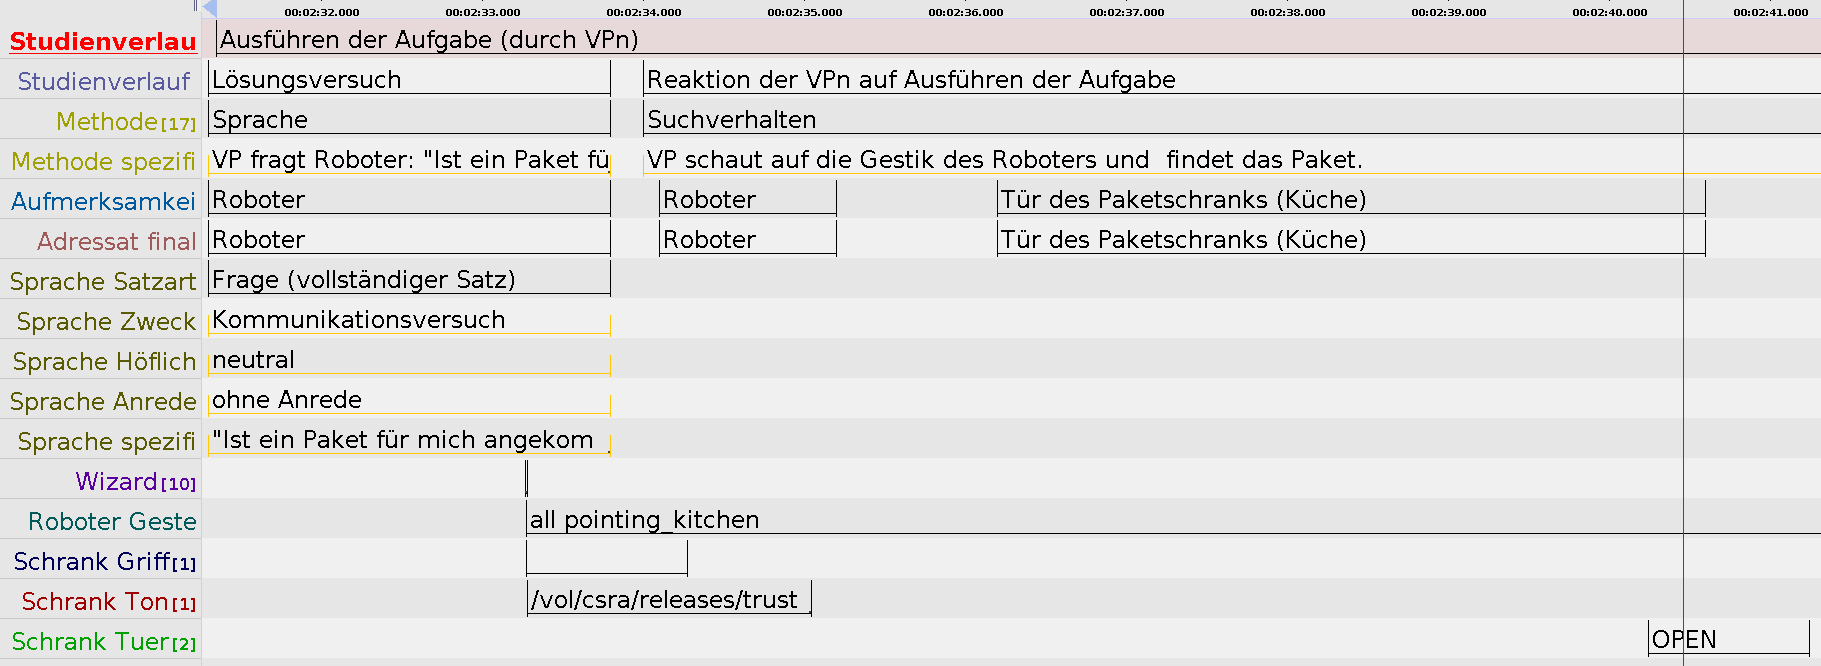
\includegraphics[trim={0 7cm 0cm 0cm},clip]{study-addressee-vp57-elan.png}
          };
         \end{tikzpicture}
       }
      \begin{footnotesize}
        \textbf{307} observations of successful communication attempts in \textbf{16} variables \vspace{10pt}
      \\\textcolor{mypurple}{\textbf{Addressee [Ar]}} \hspace{2pt} \textit{Unspecific, Parts of the Apartment, Robot, Light in the hallway  or Floor lamp}
      \pause
        \\\textcolor{myorange!50!black}{\textbf{Speech}} \hspace{2pt} Naming, Politeness, Phrasing, Sentence, Keywords
      \pause
        \\\textcolor{myyellow!50!black}{\textbf{Visual}} \hspace{2pt} FoA, Modality, Gestures, Emotions
      \pause
        \\\textcolor{mygray}{\textbf{Other}} \hspace{2pt} Id, Order, Condition, Wizard Addressee, Task
      \obcite{8-}{Holthaus2016a}
      \end{footnotesize}
\end{frame}
\begin{frame}{Addressee [Ar] Predictors}
  \begin{columns}[T] % align columns
    \begin{column}{.5\textwidth}
      \centering
      \vspace{-10pt}
      \resizebox{1.\textwidth}{!}{%
          \footnotesize
          \begin{tikzpicture}
          \action<1->{\node (a) at (0,0)
          {
            \resizebox{1.\textwidth}{!}{%
              % Created by tikzDevice version 0.12
% !TEX encoding = UTF-8 Unicode
\begin{tikzpicture}[x=1pt,y=1pt]
\definecolor{fillColor}{RGB}{255,255,255}
\path[use as bounding box,fill=fillColor,fill opacity=0.00] (0,0) rectangle (398.34,298.75);
\begin{scope}
\path[clip] ( 13.74,  0.00) rectangle (384.60,298.75);
\definecolor{drawColor}{RGB}{255,255,255}
\definecolor{fillColor}{gray}{0.98}

\path[draw=drawColor,line width= 0.6pt,line join=round,line cap=round,fill=fillColor] ( 13.74,  0.00) rectangle (384.60,298.75);
\end{scope}
\begin{scope}
\path[clip] ( 42.92, 29.18) rectangle (307.00,293.25);
\definecolor{fillColor}{gray}{0.92}

\path[fill=fillColor] ( 42.92, 29.18) rectangle (307.00,293.25);
\definecolor{drawColor}{RGB}{255,255,255}

\path[draw=drawColor,line width= 0.6pt,line join=round] ( 42.92, 38.96) --
	(307.00, 38.96);

\path[draw=drawColor,line width= 0.6pt,line join=round] ( 42.92, 55.26) --
	(307.00, 55.26);

\path[draw=drawColor,line width= 0.6pt,line join=round] ( 42.92, 71.56) --
	(307.00, 71.56);

\path[draw=drawColor,line width= 0.6pt,line join=round] ( 42.92, 87.86) --
	(307.00, 87.86);

\path[draw=drawColor,line width= 0.6pt,line join=round] ( 42.92,104.16) --
	(307.00,104.16);

\path[draw=drawColor,line width= 0.6pt,line join=round] ( 42.92,120.46) --
	(307.00,120.46);

\path[draw=drawColor,line width= 0.6pt,line join=round] ( 42.92,136.76) --
	(307.00,136.76);

\path[draw=drawColor,line width= 0.6pt,line join=round] ( 42.92,153.06) --
	(307.00,153.06);

\path[draw=drawColor,line width= 0.6pt,line join=round] ( 42.92,169.37) --
	(307.00,169.37);

\path[draw=drawColor,line width= 0.6pt,line join=round] ( 42.92,185.67) --
	(307.00,185.67);

\path[draw=drawColor,line width= 0.6pt,line join=round] ( 42.92,201.97) --
	(307.00,201.97);

\path[draw=drawColor,line width= 0.6pt,line join=round] ( 42.92,218.27) --
	(307.00,218.27);

\path[draw=drawColor,line width= 0.6pt,line join=round] ( 42.92,234.57) --
	(307.00,234.57);

\path[draw=drawColor,line width= 0.6pt,line join=round] ( 42.92,250.87) --
	(307.00,250.87);

\path[draw=drawColor,line width= 0.6pt,line join=round] ( 42.92,267.17) --
	(307.00,267.17);

\path[draw=drawColor,line width= 0.6pt,line join=round] ( 42.92,283.47) --
	(307.00,283.47);

\path[draw=drawColor,line width= 0.6pt,line join=round] ( 52.70, 29.18) --
	( 52.70,293.25);

\path[draw=drawColor,line width= 0.6pt,line join=round] ( 69.00, 29.18) --
	( 69.00,293.25);

\path[draw=drawColor,line width= 0.6pt,line join=round] ( 85.30, 29.18) --
	( 85.30,293.25);

\path[draw=drawColor,line width= 0.6pt,line join=round] (101.60, 29.18) --
	(101.60,293.25);

\path[draw=drawColor,line width= 0.6pt,line join=round] (117.90, 29.18) --
	(117.90,293.25);

\path[draw=drawColor,line width= 0.6pt,line join=round] (134.21, 29.18) --
	(134.21,293.25);

\path[draw=drawColor,line width= 0.6pt,line join=round] (150.51, 29.18) --
	(150.51,293.25);

\path[draw=drawColor,line width= 0.6pt,line join=round] (166.81, 29.18) --
	(166.81,293.25);

\path[draw=drawColor,line width= 0.6pt,line join=round] (183.11, 29.18) --
	(183.11,293.25);

\path[draw=drawColor,line width= 0.6pt,line join=round] (199.41, 29.18) --
	(199.41,293.25);

\path[draw=drawColor,line width= 0.6pt,line join=round] (215.71, 29.18) --
	(215.71,293.25);

\path[draw=drawColor,line width= 0.6pt,line join=round] (232.01, 29.18) --
	(232.01,293.25);

\path[draw=drawColor,line width= 0.6pt,line join=round] (248.31, 29.18) --
	(248.31,293.25);

\path[draw=drawColor,line width= 0.6pt,line join=round] (264.61, 29.18) --
	(264.61,293.25);

\path[draw=drawColor,line width= 0.6pt,line join=round] (280.91, 29.18) --
	(280.91,293.25);

\path[draw=drawColor,line width= 0.6pt,line join=round] (297.22, 29.18) --
	(297.22,293.25);
\definecolor{fillColor}{RGB}{5,113,176}

\path[fill=fillColor] ( 44.55, 30.81) rectangle ( 60.85, 47.11);

\path[fill=fillColor] ( 60.85, 30.81) rectangle ( 77.15, 47.11);

\path[fill=fillColor] ( 77.15, 30.81) rectangle ( 93.45, 47.11);
\definecolor{fillColor}{RGB}{244,165,130}

\path[fill=fillColor] ( 93.45, 30.81) rectangle (109.75, 47.11);
\definecolor{fillColor}{RGB}{5,113,176}

\path[fill=fillColor] (109.75, 30.81) rectangle (126.05, 47.11);

\path[fill=fillColor] (126.05, 30.81) rectangle (142.36, 47.11);

\path[fill=fillColor] (142.36, 30.81) rectangle (158.66, 47.11);

\path[fill=fillColor] (158.66, 30.81) rectangle (174.96, 47.11);

\path[fill=fillColor] (174.96, 30.81) rectangle (191.26, 47.11);

\path[fill=fillColor] (191.26, 30.81) rectangle (207.56, 47.11);

\path[fill=fillColor] (207.56, 30.81) rectangle (223.86, 47.11);

\path[fill=fillColor] (223.86, 30.81) rectangle (240.16, 47.11);

\path[fill=fillColor] (240.16, 30.81) rectangle (256.46, 47.11);
\definecolor{fillColor}{gray}{0.97}

\path[fill=fillColor] (256.46, 30.81) rectangle (272.76, 47.11);
\definecolor{fillColor}{RGB}{202,0,32}

\path[fill=fillColor] (272.76, 30.81) rectangle (289.07, 47.11);
\definecolor{fillColor}{RGB}{5,113,176}

\path[fill=fillColor] (289.07, 30.81) rectangle (305.37, 47.11);

\path[fill=fillColor] ( 44.55, 47.11) rectangle ( 60.85, 63.41);

\path[fill=fillColor] ( 60.85, 47.11) rectangle ( 77.15, 63.41);
\definecolor{fillColor}{RGB}{146,197,222}

\path[fill=fillColor] ( 77.15, 47.11) rectangle ( 93.45, 63.41);
\definecolor{fillColor}{RGB}{202,0,32}

\path[fill=fillColor] ( 93.45, 47.11) rectangle (109.75, 63.41);
\definecolor{fillColor}{RGB}{5,113,176}

\path[fill=fillColor] (109.75, 47.11) rectangle (126.05, 63.41);

\path[fill=fillColor] (126.05, 47.11) rectangle (142.36, 63.41);

\path[fill=fillColor] (142.36, 47.11) rectangle (158.66, 63.41);

\path[fill=fillColor] (158.66, 47.11) rectangle (174.96, 63.41);

\path[fill=fillColor] (174.96, 47.11) rectangle (191.26, 63.41);

\path[fill=fillColor] (191.26, 47.11) rectangle (207.56, 63.41);

\path[fill=fillColor] (207.56, 47.11) rectangle (223.86, 63.41);

\path[fill=fillColor] (223.86, 47.11) rectangle (240.16, 63.41);

\path[fill=fillColor] (240.16, 47.11) rectangle (256.46, 63.41);
\definecolor{fillColor}{gray}{0.97}

\path[fill=fillColor] (256.46, 47.11) rectangle (272.76, 63.41);

\path[fill=fillColor] (272.76, 47.11) rectangle (289.07, 63.41);
\definecolor{fillColor}{RGB}{5,113,176}

\path[fill=fillColor] (289.07, 47.11) rectangle (305.37, 63.41);

\path[fill=fillColor] ( 44.55, 63.41) rectangle ( 60.85, 79.71);
\definecolor{fillColor}{RGB}{146,197,222}

\path[fill=fillColor] ( 60.85, 63.41) rectangle ( 77.15, 79.71);
\definecolor{fillColor}{RGB}{5,113,176}

\path[fill=fillColor] ( 77.15, 63.41) rectangle ( 93.45, 79.71);
\definecolor{fillColor}{RGB}{202,0,32}

\path[fill=fillColor] ( 93.45, 63.41) rectangle (109.75, 79.71);

\path[fill=fillColor] (109.75, 63.41) rectangle (126.05, 79.71);

\path[fill=fillColor] (126.05, 63.41) rectangle (142.36, 79.71);

\path[fill=fillColor] (142.36, 63.41) rectangle (158.66, 79.71);

\path[fill=fillColor] (158.66, 63.41) rectangle (174.96, 79.71);

\path[fill=fillColor] (174.96, 63.41) rectangle (191.26, 79.71);

\path[fill=fillColor] (191.26, 63.41) rectangle (207.56, 79.71);

\path[fill=fillColor] (207.56, 63.41) rectangle (223.86, 79.71);
\definecolor{fillColor}{RGB}{244,165,130}

\path[fill=fillColor] (223.86, 63.41) rectangle (240.16, 79.71);
\definecolor{fillColor}{RGB}{202,0,32}

\path[fill=fillColor] (240.16, 63.41) rectangle (256.46, 79.71);

\path[fill=fillColor] (256.46, 63.41) rectangle (272.76, 79.71);

\path[fill=fillColor] (272.76, 63.41) rectangle (289.07, 79.71);
\definecolor{fillColor}{gray}{0.97}

\path[fill=fillColor] (289.07, 63.41) rectangle (305.37, 79.71);
\definecolor{fillColor}{RGB}{244,165,130}

\path[fill=fillColor] ( 44.55, 79.71) rectangle ( 60.85, 96.01);
\definecolor{fillColor}{RGB}{202,0,32}

\path[fill=fillColor] ( 60.85, 79.71) rectangle ( 77.15, 96.01);

\path[fill=fillColor] ( 77.15, 79.71) rectangle ( 93.45, 96.01);
\definecolor{fillColor}{RGB}{5,113,176}

\path[fill=fillColor] ( 93.45, 79.71) rectangle (109.75, 96.01);
\definecolor{fillColor}{RGB}{202,0,32}

\path[fill=fillColor] (109.75, 79.71) rectangle (126.05, 96.01);

\path[fill=fillColor] (126.05, 79.71) rectangle (142.36, 96.01);
\definecolor{fillColor}{RGB}{146,197,222}

\path[fill=fillColor] (142.36, 79.71) rectangle (158.66, 96.01);
\definecolor{fillColor}{RGB}{202,0,32}

\path[fill=fillColor] (158.66, 79.71) rectangle (174.96, 96.01);

\path[fill=fillColor] (174.96, 79.71) rectangle (191.26, 96.01);

\path[fill=fillColor] (191.26, 79.71) rectangle (207.56, 96.01);
\definecolor{fillColor}{gray}{0.97}

\path[fill=fillColor] (207.56, 79.71) rectangle (223.86, 96.01);

\path[fill=fillColor] (223.86, 79.71) rectangle (240.16, 96.01);

\path[fill=fillColor] (240.16, 79.71) rectangle (256.46, 96.01);
\definecolor{fillColor}{RGB}{202,0,32}

\path[fill=fillColor] (256.46, 79.71) rectangle (272.76, 96.01);
\definecolor{fillColor}{gray}{0.97}

\path[fill=fillColor] (272.76, 79.71) rectangle (289.07, 96.01);
\definecolor{fillColor}{RGB}{146,197,222}

\path[fill=fillColor] (289.07, 79.71) rectangle (305.37, 96.01);
\definecolor{fillColor}{RGB}{5,113,176}

\path[fill=fillColor] ( 44.55, 96.01) rectangle ( 60.85,112.31);

\path[fill=fillColor] ( 60.85, 96.01) rectangle ( 77.15,112.31);
\definecolor{fillColor}{RGB}{202,0,32}

\path[fill=fillColor] ( 77.15, 96.01) rectangle ( 93.45,112.31);

\path[fill=fillColor] ( 93.45, 96.01) rectangle (109.75,112.31);
\definecolor{fillColor}{RGB}{5,113,176}

\path[fill=fillColor] (109.75, 96.01) rectangle (126.05,112.31);

\path[fill=fillColor] (126.05, 96.01) rectangle (142.36,112.31);

\path[fill=fillColor] (142.36, 96.01) rectangle (158.66,112.31);

\path[fill=fillColor] (158.66, 96.01) rectangle (174.96,112.31);

\path[fill=fillColor] (174.96, 96.01) rectangle (191.26,112.31);

\path[fill=fillColor] (191.26, 96.01) rectangle (207.56,112.31);

\path[fill=fillColor] (207.56, 96.01) rectangle (223.86,112.31);

\path[fill=fillColor] (223.86, 96.01) rectangle (240.16,112.31);

\path[fill=fillColor] (240.16, 96.01) rectangle (256.46,112.31);
\definecolor{fillColor}{RGB}{202,0,32}

\path[fill=fillColor] (256.46, 96.01) rectangle (272.76,112.31);
\definecolor{fillColor}{RGB}{5,113,176}

\path[fill=fillColor] (272.76, 96.01) rectangle (289.07,112.31);

\path[fill=fillColor] (289.07, 96.01) rectangle (305.37,112.31);

\path[fill=fillColor] ( 44.55,112.31) rectangle ( 60.85,128.61);

\path[fill=fillColor] ( 60.85,112.31) rectangle ( 77.15,128.61);
\definecolor{fillColor}{RGB}{202,0,32}

\path[fill=fillColor] ( 77.15,112.31) rectangle ( 93.45,128.61);

\path[fill=fillColor] ( 93.45,112.31) rectangle (109.75,128.61);
\definecolor{fillColor}{RGB}{5,113,176}

\path[fill=fillColor] (109.75,112.31) rectangle (126.05,128.61);

\path[fill=fillColor] (126.05,112.31) rectangle (142.36,128.61);

\path[fill=fillColor] (142.36,112.31) rectangle (158.66,128.61);

\path[fill=fillColor] (158.66,112.31) rectangle (174.96,128.61);

\path[fill=fillColor] (174.96,112.31) rectangle (191.26,128.61);

\path[fill=fillColor] (191.26,112.31) rectangle (207.56,128.61);
\definecolor{fillColor}{RGB}{202,0,32}

\path[fill=fillColor] (207.56,112.31) rectangle (223.86,128.61);
\definecolor{fillColor}{RGB}{146,197,222}

\path[fill=fillColor] (223.86,112.31) rectangle (240.16,128.61);
\definecolor{fillColor}{gray}{0.97}

\path[fill=fillColor] (240.16,112.31) rectangle (256.46,128.61);
\definecolor{fillColor}{RGB}{202,0,32}

\path[fill=fillColor] (256.46,112.31) rectangle (272.76,128.61);
\definecolor{fillColor}{RGB}{5,113,176}

\path[fill=fillColor] (272.76,112.31) rectangle (289.07,128.61);

\path[fill=fillColor] (289.07,112.31) rectangle (305.37,128.61);

\path[fill=fillColor] ( 44.55,128.61) rectangle ( 60.85,144.91);

\path[fill=fillColor] ( 60.85,128.61) rectangle ( 77.15,144.91);
\definecolor{fillColor}{RGB}{202,0,32}

\path[fill=fillColor] ( 77.15,128.61) rectangle ( 93.45,144.91);
\definecolor{fillColor}{RGB}{146,197,222}

\path[fill=fillColor] ( 93.45,128.61) rectangle (109.75,144.91);
\definecolor{fillColor}{RGB}{5,113,176}

\path[fill=fillColor] (109.75,128.61) rectangle (126.05,144.91);

\path[fill=fillColor] (126.05,128.61) rectangle (142.36,144.91);

\path[fill=fillColor] (142.36,128.61) rectangle (158.66,144.91);

\path[fill=fillColor] (158.66,128.61) rectangle (174.96,144.91);

\path[fill=fillColor] (174.96,128.61) rectangle (191.26,144.91);

\path[fill=fillColor] (191.26,128.61) rectangle (207.56,144.91);

\path[fill=fillColor] (207.56,128.61) rectangle (223.86,144.91);

\path[fill=fillColor] (223.86,128.61) rectangle (240.16,144.91);

\path[fill=fillColor] (240.16,128.61) rectangle (256.46,144.91);
\definecolor{fillColor}{RGB}{202,0,32}

\path[fill=fillColor] (256.46,128.61) rectangle (272.76,144.91);
\definecolor{fillColor}{RGB}{5,113,176}

\path[fill=fillColor] (272.76,128.61) rectangle (289.07,144.91);

\path[fill=fillColor] (289.07,128.61) rectangle (305.37,144.91);

\path[fill=fillColor] ( 44.55,144.91) rectangle ( 60.85,161.22);

\path[fill=fillColor] ( 60.85,144.91) rectangle ( 77.15,161.22);
\definecolor{fillColor}{RGB}{202,0,32}

\path[fill=fillColor] ( 77.15,144.91) rectangle ( 93.45,161.22);

\path[fill=fillColor] ( 93.45,144.91) rectangle (109.75,161.22);
\definecolor{fillColor}{RGB}{5,113,176}

\path[fill=fillColor] (109.75,144.91) rectangle (126.05,161.22);

\path[fill=fillColor] (126.05,144.91) rectangle (142.36,161.22);

\path[fill=fillColor] (142.36,144.91) rectangle (158.66,161.22);

\path[fill=fillColor] (158.66,144.91) rectangle (174.96,161.22);

\path[fill=fillColor] (174.96,144.91) rectangle (191.26,161.22);

\path[fill=fillColor] (191.26,144.91) rectangle (207.56,161.22);

\path[fill=fillColor] (207.56,144.91) rectangle (223.86,161.22);

\path[fill=fillColor] (223.86,144.91) rectangle (240.16,161.22);

\path[fill=fillColor] (240.16,144.91) rectangle (256.46,161.22);
\definecolor{fillColor}{RGB}{244,165,130}

\path[fill=fillColor] (256.46,144.91) rectangle (272.76,161.22);
\definecolor{fillColor}{RGB}{5,113,176}

\path[fill=fillColor] (272.76,144.91) rectangle (289.07,161.22);

\path[fill=fillColor] (289.07,144.91) rectangle (305.37,161.22);

\path[fill=fillColor] ( 44.55,161.22) rectangle ( 60.85,177.52);

\path[fill=fillColor] ( 60.85,161.22) rectangle ( 77.15,177.52);
\definecolor{fillColor}{RGB}{202,0,32}

\path[fill=fillColor] ( 77.15,161.22) rectangle ( 93.45,177.52);

\path[fill=fillColor] ( 93.45,161.22) rectangle (109.75,177.52);
\definecolor{fillColor}{RGB}{5,113,176}

\path[fill=fillColor] (109.75,161.22) rectangle (126.05,177.52);

\path[fill=fillColor] (126.05,161.22) rectangle (142.36,177.52);

\path[fill=fillColor] (142.36,161.22) rectangle (158.66,177.52);

\path[fill=fillColor] (158.66,161.22) rectangle (174.96,177.52);

\path[fill=fillColor] (174.96,161.22) rectangle (191.26,177.52);

\path[fill=fillColor] (191.26,161.22) rectangle (207.56,177.52);

\path[fill=fillColor] (207.56,161.22) rectangle (223.86,177.52);

\path[fill=fillColor] (223.86,161.22) rectangle (240.16,177.52);

\path[fill=fillColor] (240.16,161.22) rectangle (256.46,177.52);
\definecolor{fillColor}{RGB}{202,0,32}

\path[fill=fillColor] (256.46,161.22) rectangle (272.76,177.52);
\definecolor{fillColor}{RGB}{5,113,176}

\path[fill=fillColor] (272.76,161.22) rectangle (289.07,177.52);
\definecolor{fillColor}{RGB}{146,197,222}

\path[fill=fillColor] (289.07,161.22) rectangle (305.37,177.52);
\definecolor{fillColor}{RGB}{5,113,176}

\path[fill=fillColor] ( 44.55,177.52) rectangle ( 60.85,193.82);

\path[fill=fillColor] ( 60.85,177.52) rectangle ( 77.15,193.82);
\definecolor{fillColor}{RGB}{202,0,32}

\path[fill=fillColor] ( 77.15,177.52) rectangle ( 93.45,193.82);

\path[fill=fillColor] ( 93.45,177.52) rectangle (109.75,193.82);
\definecolor{fillColor}{RGB}{5,113,176}

\path[fill=fillColor] (109.75,177.52) rectangle (126.05,193.82);

\path[fill=fillColor] (126.05,177.52) rectangle (142.36,193.82);

\path[fill=fillColor] (142.36,177.52) rectangle (158.66,193.82);

\path[fill=fillColor] (158.66,177.52) rectangle (174.96,193.82);

\path[fill=fillColor] (174.96,177.52) rectangle (191.26,193.82);

\path[fill=fillColor] (191.26,177.52) rectangle (207.56,193.82);

\path[fill=fillColor] (207.56,177.52) rectangle (223.86,193.82);

\path[fill=fillColor] (223.86,177.52) rectangle (240.16,193.82);

\path[fill=fillColor] (240.16,177.52) rectangle (256.46,193.82);
\definecolor{fillColor}{RGB}{202,0,32}

\path[fill=fillColor] (256.46,177.52) rectangle (272.76,193.82);
\definecolor{fillColor}{RGB}{5,113,176}

\path[fill=fillColor] (272.76,177.52) rectangle (289.07,193.82);

\path[fill=fillColor] (289.07,177.52) rectangle (305.37,193.82);

\path[fill=fillColor] ( 44.55,193.82) rectangle ( 60.85,210.12);

\path[fill=fillColor] ( 60.85,193.82) rectangle ( 77.15,210.12);
\definecolor{fillColor}{RGB}{202,0,32}

\path[fill=fillColor] ( 77.15,193.82) rectangle ( 93.45,210.12);
\definecolor{fillColor}{gray}{0.97}

\path[fill=fillColor] ( 93.45,193.82) rectangle (109.75,210.12);
\definecolor{fillColor}{RGB}{5,113,176}

\path[fill=fillColor] (109.75,193.82) rectangle (126.05,210.12);
\definecolor{fillColor}{RGB}{202,0,32}

\path[fill=fillColor] (126.05,193.82) rectangle (142.36,210.12);
\definecolor{fillColor}{RGB}{5,113,176}

\path[fill=fillColor] (142.36,193.82) rectangle (158.66,210.12);

\path[fill=fillColor] (158.66,193.82) rectangle (174.96,210.12);

\path[fill=fillColor] (174.96,193.82) rectangle (191.26,210.12);

\path[fill=fillColor] (191.26,193.82) rectangle (207.56,210.12);

\path[fill=fillColor] (207.56,193.82) rectangle (223.86,210.12);

\path[fill=fillColor] (223.86,193.82) rectangle (240.16,210.12);

\path[fill=fillColor] (240.16,193.82) rectangle (256.46,210.12);
\definecolor{fillColor}{RGB}{146,197,222}

\path[fill=fillColor] (256.46,193.82) rectangle (272.76,210.12);

\path[fill=fillColor] (272.76,193.82) rectangle (289.07,210.12);
\definecolor{fillColor}{RGB}{5,113,176}

\path[fill=fillColor] (289.07,193.82) rectangle (305.37,210.12);

\path[fill=fillColor] ( 44.55,210.12) rectangle ( 60.85,226.42);

\path[fill=fillColor] ( 60.85,210.12) rectangle ( 77.15,226.42);
\definecolor{fillColor}{RGB}{244,165,130}

\path[fill=fillColor] ( 77.15,210.12) rectangle ( 93.45,226.42);
\definecolor{fillColor}{gray}{0.97}

\path[fill=fillColor] ( 93.45,210.12) rectangle (109.75,226.42);
\definecolor{fillColor}{RGB}{5,113,176}

\path[fill=fillColor] (109.75,210.12) rectangle (126.05,226.42);
\definecolor{fillColor}{RGB}{146,197,222}

\path[fill=fillColor] (126.05,210.12) rectangle (142.36,226.42);
\definecolor{fillColor}{RGB}{5,113,176}

\path[fill=fillColor] (142.36,210.12) rectangle (158.66,226.42);

\path[fill=fillColor] (158.66,210.12) rectangle (174.96,226.42);

\path[fill=fillColor] (174.96,210.12) rectangle (191.26,226.42);

\path[fill=fillColor] (191.26,210.12) rectangle (207.56,226.42);

\path[fill=fillColor] (207.56,210.12) rectangle (223.86,226.42);

\path[fill=fillColor] (223.86,210.12) rectangle (240.16,226.42);

\path[fill=fillColor] (240.16,210.12) rectangle (256.46,226.42);
\definecolor{fillColor}{RGB}{244,165,130}

\path[fill=fillColor] (256.46,210.12) rectangle (272.76,226.42);
\definecolor{fillColor}{RGB}{202,0,32}

\path[fill=fillColor] (272.76,210.12) rectangle (289.07,226.42);
\definecolor{fillColor}{RGB}{5,113,176}

\path[fill=fillColor] (289.07,210.12) rectangle (305.37,226.42);

\path[fill=fillColor] ( 44.55,226.42) rectangle ( 60.85,242.72);

\path[fill=fillColor] ( 60.85,226.42) rectangle ( 77.15,242.72);
\definecolor{fillColor}{RGB}{202,0,32}

\path[fill=fillColor] ( 77.15,226.42) rectangle ( 93.45,242.72);
\definecolor{fillColor}{gray}{0.97}

\path[fill=fillColor] ( 93.45,226.42) rectangle (109.75,242.72);
\definecolor{fillColor}{RGB}{5,113,176}

\path[fill=fillColor] (109.75,226.42) rectangle (126.05,242.72);
\definecolor{fillColor}{gray}{0.97}

\path[fill=fillColor] (126.05,226.42) rectangle (142.36,242.72);
\definecolor{fillColor}{RGB}{5,113,176}

\path[fill=fillColor] (142.36,226.42) rectangle (158.66,242.72);

\path[fill=fillColor] (158.66,226.42) rectangle (174.96,242.72);

\path[fill=fillColor] (174.96,226.42) rectangle (191.26,242.72);

\path[fill=fillColor] (191.26,226.42) rectangle (207.56,242.72);

\path[fill=fillColor] (207.56,226.42) rectangle (223.86,242.72);

\path[fill=fillColor] (223.86,226.42) rectangle (240.16,242.72);

\path[fill=fillColor] (240.16,226.42) rectangle (256.46,242.72);
\definecolor{fillColor}{RGB}{202,0,32}

\path[fill=fillColor] (256.46,226.42) rectangle (272.76,242.72);

\path[fill=fillColor] (272.76,226.42) rectangle (289.07,242.72);

\path[fill=fillColor] (289.07,226.42) rectangle (305.37,242.72);
\definecolor{fillColor}{gray}{0.97}

\path[fill=fillColor] ( 44.55,242.72) rectangle ( 60.85,259.02);

\path[fill=fillColor] ( 60.85,242.72) rectangle ( 77.15,259.02);
\definecolor{fillColor}{RGB}{202,0,32}

\path[fill=fillColor] ( 77.15,242.72) rectangle ( 93.45,259.02);

\path[fill=fillColor] ( 93.45,242.72) rectangle (109.75,259.02);

\path[fill=fillColor] (109.75,242.72) rectangle (126.05,259.02);

\path[fill=fillColor] (126.05,242.72) rectangle (142.36,259.02);

\path[fill=fillColor] (142.36,242.72) rectangle (158.66,259.02);
\definecolor{fillColor}{RGB}{244,165,130}

\path[fill=fillColor] (158.66,242.72) rectangle (174.96,259.02);
\definecolor{fillColor}{RGB}{202,0,32}

\path[fill=fillColor] (174.96,242.72) rectangle (191.26,259.02);

\path[fill=fillColor] (191.26,242.72) rectangle (207.56,259.02);
\definecolor{fillColor}{RGB}{146,197,222}

\path[fill=fillColor] (207.56,242.72) rectangle (223.86,259.02);
\definecolor{fillColor}{RGB}{244,165,130}

\path[fill=fillColor] (223.86,242.72) rectangle (240.16,259.02);
\definecolor{fillColor}{RGB}{202,0,32}

\path[fill=fillColor] (240.16,242.72) rectangle (256.46,259.02);
\definecolor{fillColor}{RGB}{5,113,176}

\path[fill=fillColor] (256.46,242.72) rectangle (272.76,259.02);
\definecolor{fillColor}{RGB}{146,197,222}

\path[fill=fillColor] (272.76,242.72) rectangle (289.07,259.02);
\definecolor{fillColor}{RGB}{5,113,176}

\path[fill=fillColor] (289.07,242.72) rectangle (305.37,259.02);
\definecolor{fillColor}{RGB}{202,0,32}

\path[fill=fillColor] ( 44.55,259.02) rectangle ( 60.85,275.32);
\definecolor{fillColor}{gray}{0.97}

\path[fill=fillColor] ( 60.85,259.02) rectangle ( 77.15,275.32);
\definecolor{fillColor}{RGB}{202,0,32}

\path[fill=fillColor] ( 77.15,259.02) rectangle ( 93.45,275.32);
\definecolor{fillColor}{gray}{0.97}

\path[fill=fillColor] ( 93.45,259.02) rectangle (109.75,275.32);
\definecolor{fillColor}{RGB}{5,113,176}

\path[fill=fillColor] (109.75,259.02) rectangle (126.05,275.32);

\path[fill=fillColor] (126.05,259.02) rectangle (142.36,275.32);

\path[fill=fillColor] (142.36,259.02) rectangle (158.66,275.32);

\path[fill=fillColor] (158.66,259.02) rectangle (174.96,275.32);

\path[fill=fillColor] (174.96,259.02) rectangle (191.26,275.32);

\path[fill=fillColor] (191.26,259.02) rectangle (207.56,275.32);
\definecolor{fillColor}{RGB}{146,197,222}

\path[fill=fillColor] (207.56,259.02) rectangle (223.86,275.32);
\definecolor{fillColor}{RGB}{202,0,32}

\path[fill=fillColor] (223.86,259.02) rectangle (240.16,275.32);

\path[fill=fillColor] (240.16,259.02) rectangle (256.46,275.32);
\definecolor{fillColor}{RGB}{146,197,222}

\path[fill=fillColor] (256.46,259.02) rectangle (272.76,275.32);
\definecolor{fillColor}{RGB}{5,113,176}

\path[fill=fillColor] (272.76,259.02) rectangle (289.07,275.32);

\path[fill=fillColor] (289.07,259.02) rectangle (305.37,275.32);

\path[fill=fillColor] ( 44.55,275.32) rectangle ( 60.85,291.62);

\path[fill=fillColor] ( 60.85,275.32) rectangle ( 77.15,291.62);
\definecolor{fillColor}{gray}{0.97}

\path[fill=fillColor] ( 77.15,275.32) rectangle ( 93.45,291.62);
\definecolor{fillColor}{RGB}{146,197,222}

\path[fill=fillColor] ( 93.45,275.32) rectangle (109.75,291.62);
\definecolor{fillColor}{RGB}{5,113,176}

\path[fill=fillColor] (109.75,275.32) rectangle (126.05,291.62);

\path[fill=fillColor] (126.05,275.32) rectangle (142.36,291.62);

\path[fill=fillColor] (142.36,275.32) rectangle (158.66,291.62);

\path[fill=fillColor] (158.66,275.32) rectangle (174.96,291.62);
\definecolor{fillColor}{RGB}{146,197,222}

\path[fill=fillColor] (174.96,275.32) rectangle (191.26,291.62);
\definecolor{fillColor}{RGB}{5,113,176}

\path[fill=fillColor] (191.26,275.32) rectangle (207.56,291.62);

\path[fill=fillColor] (207.56,275.32) rectangle (223.86,291.62);

\path[fill=fillColor] (223.86,275.32) rectangle (240.16,291.62);
\definecolor{fillColor}{RGB}{202,0,32}

\path[fill=fillColor] (240.16,275.32) rectangle (256.46,291.62);
\definecolor{fillColor}{RGB}{5,113,176}

\path[fill=fillColor] (256.46,275.32) rectangle (272.76,291.62);

\path[fill=fillColor] (272.76,275.32) rectangle (289.07,291.62);

\path[fill=fillColor] (289.07,275.32) rectangle (305.37,291.62);
\end{scope}
\begin{scope}
\path[clip] (  0.00,  0.00) rectangle (398.34,298.75);
\definecolor{drawColor}{RGB}{0,0,0}

\node[text=drawColor,anchor=base east,inner sep=0pt, outer sep=0pt, scale=  1.10] at ( 37.97, 35.17) {Ar};

\node[text=drawColor,anchor=base east,inner sep=0pt, outer sep=0pt, scale=  1.10] at ( 37.97, 51.47) {Fr};

\node[text=drawColor,anchor=base east,inner sep=0pt, outer sep=0pt, scale=  1.10] at ( 37.97, 67.77) {Aef};

\node[text=drawColor,anchor=base east,inner sep=0pt, outer sep=0pt, scale=  1.10] at ( 37.97, 84.07) {Er};

\node[text=drawColor,anchor=base east,inner sep=0pt, outer sep=0pt, scale=  1.10] at ( 37.97,100.37) {M};

\node[text=drawColor,anchor=base east,inner sep=0pt, outer sep=0pt, scale=  1.10] at ( 37.97,116.67) {Msr};

\node[text=drawColor,anchor=base east,inner sep=0pt, outer sep=0pt, scale=  1.10] at ( 37.97,132.98) {Sf};

\node[text=drawColor,anchor=base east,inner sep=0pt, outer sep=0pt, scale=  1.10] at ( 37.97,149.28) {Sp};

\node[text=drawColor,anchor=base east,inner sep=0pt, outer sep=0pt, scale=  1.10] at ( 37.97,165.58) {Str};

\node[text=drawColor,anchor=base east,inner sep=0pt, outer sep=0pt, scale=  1.10] at ( 37.97,181.88) {Sph};

\node[text=drawColor,anchor=base east,inner sep=0pt, outer sep=0pt, scale=  1.10] at ( 37.97,198.18) {Ssr};

\node[text=drawColor,anchor=base east,inner sep=0pt, outer sep=0pt, scale=  1.10] at ( 37.97,214.48) {Aw};

\node[text=drawColor,anchor=base east,inner sep=0pt, outer sep=0pt, scale=  1.10] at ( 37.97,230.78) {T};

\node[text=drawColor,anchor=base east,inner sep=0pt, outer sep=0pt, scale=  1.10] at ( 37.97,247.08) {C};

\node[text=drawColor,anchor=base east,inner sep=0pt, outer sep=0pt, scale=  1.10] at ( 37.97,263.38) {O};

\node[text=drawColor,anchor=base east,inner sep=0pt, outer sep=0pt, scale=  1.10] at ( 37.97,279.69) {Pid};
\end{scope}
\begin{scope}
\path[clip] (  0.00,  0.00) rectangle (398.34,298.75);
\definecolor{drawColor}{gray}{0.20}

\path[draw=drawColor,line width= 0.6pt,line join=round] ( 40.17, 38.96) --
	( 42.92, 38.96);

\path[draw=drawColor,line width= 0.6pt,line join=round] ( 40.17, 55.26) --
	( 42.92, 55.26);

\path[draw=drawColor,line width= 0.6pt,line join=round] ( 40.17, 71.56) --
	( 42.92, 71.56);

\path[draw=drawColor,line width= 0.6pt,line join=round] ( 40.17, 87.86) --
	( 42.92, 87.86);

\path[draw=drawColor,line width= 0.6pt,line join=round] ( 40.17,104.16) --
	( 42.92,104.16);

\path[draw=drawColor,line width= 0.6pt,line join=round] ( 40.17,120.46) --
	( 42.92,120.46);

\path[draw=drawColor,line width= 0.6pt,line join=round] ( 40.17,136.76) --
	( 42.92,136.76);

\path[draw=drawColor,line width= 0.6pt,line join=round] ( 40.17,153.06) --
	( 42.92,153.06);

\path[draw=drawColor,line width= 0.6pt,line join=round] ( 40.17,169.37) --
	( 42.92,169.37);

\path[draw=drawColor,line width= 0.6pt,line join=round] ( 40.17,185.67) --
	( 42.92,185.67);

\path[draw=drawColor,line width= 0.6pt,line join=round] ( 40.17,201.97) --
	( 42.92,201.97);

\path[draw=drawColor,line width= 0.6pt,line join=round] ( 40.17,218.27) --
	( 42.92,218.27);

\path[draw=drawColor,line width= 0.6pt,line join=round] ( 40.17,234.57) --
	( 42.92,234.57);

\path[draw=drawColor,line width= 0.6pt,line join=round] ( 40.17,250.87) --
	( 42.92,250.87);

\path[draw=drawColor,line width= 0.6pt,line join=round] ( 40.17,267.17) --
	( 42.92,267.17);

\path[draw=drawColor,line width= 0.6pt,line join=round] ( 40.17,283.47) --
	( 42.92,283.47);
\end{scope}
\begin{scope}
\path[clip] (  0.00,  0.00) rectangle (398.34,298.75);
\definecolor{drawColor}{gray}{0.20}

\path[draw=drawColor,line width= 0.6pt,line join=round] ( 52.70, 26.43) --
	( 52.70, 29.18);

\path[draw=drawColor,line width= 0.6pt,line join=round] ( 69.00, 26.43) --
	( 69.00, 29.18);

\path[draw=drawColor,line width= 0.6pt,line join=round] ( 85.30, 26.43) --
	( 85.30, 29.18);

\path[draw=drawColor,line width= 0.6pt,line join=round] (101.60, 26.43) --
	(101.60, 29.18);

\path[draw=drawColor,line width= 0.6pt,line join=round] (117.90, 26.43) --
	(117.90, 29.18);

\path[draw=drawColor,line width= 0.6pt,line join=round] (134.21, 26.43) --
	(134.21, 29.18);

\path[draw=drawColor,line width= 0.6pt,line join=round] (150.51, 26.43) --
	(150.51, 29.18);

\path[draw=drawColor,line width= 0.6pt,line join=round] (166.81, 26.43) --
	(166.81, 29.18);

\path[draw=drawColor,line width= 0.6pt,line join=round] (183.11, 26.43) --
	(183.11, 29.18);

\path[draw=drawColor,line width= 0.6pt,line join=round] (199.41, 26.43) --
	(199.41, 29.18);

\path[draw=drawColor,line width= 0.6pt,line join=round] (215.71, 26.43) --
	(215.71, 29.18);

\path[draw=drawColor,line width= 0.6pt,line join=round] (232.01, 26.43) --
	(232.01, 29.18);

\path[draw=drawColor,line width= 0.6pt,line join=round] (248.31, 26.43) --
	(248.31, 29.18);

\path[draw=drawColor,line width= 0.6pt,line join=round] (264.61, 26.43) --
	(264.61, 29.18);

\path[draw=drawColor,line width= 0.6pt,line join=round] (280.91, 26.43) --
	(280.91, 29.18);

\path[draw=drawColor,line width= 0.6pt,line join=round] (297.22, 26.43) --
	(297.22, 29.18);
\end{scope}
\begin{scope}
\path[clip] (  0.00,  0.00) rectangle (398.34,298.75);
\definecolor{drawColor}{RGB}{0,0,0}

\node[text=drawColor,rotate= 90.00,anchor=base east,inner sep=0pt, outer sep=0pt, scale=  1.10] at ( 60.28, 24.23) {Ar};

\node[text=drawColor,rotate= 90.00,anchor=base east,inner sep=0pt, outer sep=0pt, scale=  1.10] at ( 76.58, 24.23) {Fr};

\node[text=drawColor,rotate= 90.00,anchor=base east,inner sep=0pt, outer sep=0pt, scale=  1.10] at ( 92.88, 24.23) {Aef};

\node[text=drawColor,rotate= 90.00,anchor=base east,inner sep=0pt, outer sep=0pt, scale=  1.10] at (109.18, 24.23) {Er};

\node[text=drawColor,rotate= 90.00,anchor=base east,inner sep=0pt, outer sep=0pt, scale=  1.10] at (125.48, 24.23) {M};

\node[text=drawColor,rotate= 90.00,anchor=base east,inner sep=0pt, outer sep=0pt, scale=  1.10] at (141.78, 24.23) {Msr};

\node[text=drawColor,rotate= 90.00,anchor=base east,inner sep=0pt, outer sep=0pt, scale=  1.10] at (158.08, 24.23) {Sf};

\node[text=drawColor,rotate= 90.00,anchor=base east,inner sep=0pt, outer sep=0pt, scale=  1.10] at (174.38, 24.23) {Sp};

\node[text=drawColor,rotate= 90.00,anchor=base east,inner sep=0pt, outer sep=0pt, scale=  1.10] at (190.68, 24.23) {Str};

\node[text=drawColor,rotate= 90.00,anchor=base east,inner sep=0pt, outer sep=0pt, scale=  1.10] at (206.99, 24.23) {Sph};

\node[text=drawColor,rotate= 90.00,anchor=base east,inner sep=0pt, outer sep=0pt, scale=  1.10] at (223.29, 24.23) {Ssr};

\node[text=drawColor,rotate= 90.00,anchor=base east,inner sep=0pt, outer sep=0pt, scale=  1.10] at (239.59, 24.23) {Aw};

\node[text=drawColor,rotate= 90.00,anchor=base east,inner sep=0pt, outer sep=0pt, scale=  1.10] at (255.89, 24.23) {T};

\node[text=drawColor,rotate= 90.00,anchor=base east,inner sep=0pt, outer sep=0pt, scale=  1.10] at (272.19, 24.23) {C};

\node[text=drawColor,rotate= 90.00,anchor=base east,inner sep=0pt, outer sep=0pt, scale=  1.10] at (288.49, 24.23) {O};

\node[text=drawColor,rotate= 90.00,anchor=base east,inner sep=0pt, outer sep=0pt, scale=  1.10] at (304.79, 24.23) {Pid};
\end{scope}
\begin{scope}
\path[clip] (  0.00,  0.00) rectangle (398.34,298.75);
\definecolor{fillColor}{RGB}{255,255,255}

\path[fill=fillColor] (318.00,112.07) rectangle (379.10,210.36);
\end{scope}
\begin{scope}
\path[clip] (  0.00,  0.00) rectangle (398.34,298.75);
\definecolor{drawColor}{RGB}{0,0,0}

\node[text=drawColor,anchor=base west,inner sep=0pt, outer sep=0pt, scale=  1.10] at (323.50,196.31) {Sign. level};
\end{scope}
\begin{scope}
\path[clip] (  0.00,  0.00) rectangle (398.34,298.75);
\definecolor{drawColor}{RGB}{255,255,255}
\definecolor{fillColor}{gray}{0.95}

\path[draw=drawColor,line width= 0.6pt,line join=round,line cap=round,fill=fillColor] (323.50,175.39) rectangle (337.95,189.84);
\end{scope}
\begin{scope}
\path[clip] (  0.00,  0.00) rectangle (398.34,298.75);
\definecolor{fillColor}{RGB}{202,0,32}

\path[fill=fillColor] (323.64,175.53) rectangle (337.81,189.70);
\end{scope}
\begin{scope}
\path[clip] (  0.00,  0.00) rectangle (398.34,298.75);
\definecolor{drawColor}{RGB}{255,255,255}
\definecolor{fillColor}{gray}{0.95}

\path[draw=drawColor,line width= 0.6pt,line join=round,line cap=round,fill=fillColor] (323.50,160.93) rectangle (337.95,175.39);
\end{scope}
\begin{scope}
\path[clip] (  0.00,  0.00) rectangle (398.34,298.75);
\definecolor{fillColor}{RGB}{244,165,130}

\path[fill=fillColor] (323.64,161.07) rectangle (337.81,175.24);
\end{scope}
\begin{scope}
\path[clip] (  0.00,  0.00) rectangle (398.34,298.75);
\definecolor{drawColor}{RGB}{255,255,255}
\definecolor{fillColor}{gray}{0.95}

\path[draw=drawColor,line width= 0.6pt,line join=round,line cap=round,fill=fillColor] (323.50,146.48) rectangle (337.95,160.93);
\end{scope}
\begin{scope}
\path[clip] (  0.00,  0.00) rectangle (398.34,298.75);
\definecolor{fillColor}{gray}{0.97}

\path[fill=fillColor] (323.64,146.62) rectangle (337.81,160.79);
\end{scope}
\begin{scope}
\path[clip] (  0.00,  0.00) rectangle (398.34,298.75);
\definecolor{drawColor}{RGB}{255,255,255}
\definecolor{fillColor}{gray}{0.95}

\path[draw=drawColor,line width= 0.6pt,line join=round,line cap=round,fill=fillColor] (323.50,132.02) rectangle (337.95,146.48);
\end{scope}
\begin{scope}
\path[clip] (  0.00,  0.00) rectangle (398.34,298.75);
\definecolor{fillColor}{RGB}{146,197,222}

\path[fill=fillColor] (323.64,132.17) rectangle (337.81,146.34);
\end{scope}
\begin{scope}
\path[clip] (  0.00,  0.00) rectangle (398.34,298.75);
\definecolor{drawColor}{RGB}{255,255,255}
\definecolor{fillColor}{gray}{0.95}

\path[draw=drawColor,line width= 0.6pt,line join=round,line cap=round,fill=fillColor] (323.50,117.57) rectangle (337.95,132.02);
\end{scope}
\begin{scope}
\path[clip] (  0.00,  0.00) rectangle (398.34,298.75);
\definecolor{fillColor}{RGB}{5,113,176}

\path[fill=fillColor] (323.64,117.71) rectangle (337.81,131.88);
\end{scope}
\begin{scope}
\path[clip] (  0.00,  0.00) rectangle (398.34,298.75);
\definecolor{drawColor}{RGB}{0,0,0}

\node[text=drawColor,anchor=base west,inner sep=0pt, outer sep=0pt, scale=  0.88] at (343.45,179.58) {\( \leq 1\)};
\end{scope}
\begin{scope}
\path[clip] (  0.00,  0.00) rectangle (398.34,298.75);
\definecolor{drawColor}{RGB}{0,0,0}

\node[text=drawColor,anchor=base west,inner sep=0pt, outer sep=0pt, scale=  0.88] at (343.45,165.13) {\(< 0.1\)};
\end{scope}
\begin{scope}
\path[clip] (  0.00,  0.00) rectangle (398.34,298.75);
\definecolor{drawColor}{RGB}{0,0,0}

\node[text=drawColor,anchor=base west,inner sep=0pt, outer sep=0pt, scale=  0.88] at (343.45,150.67) {\(< 0.05\)};
\end{scope}
\begin{scope}
\path[clip] (  0.00,  0.00) rectangle (398.34,298.75);
\definecolor{drawColor}{RGB}{0,0,0}

\node[text=drawColor,anchor=base west,inner sep=0pt, outer sep=0pt, scale=  0.88] at (343.45,136.22) {\(< 0.01\)};
\end{scope}
\begin{scope}
\path[clip] (  0.00,  0.00) rectangle (398.34,298.75);
\definecolor{drawColor}{RGB}{0,0,0}

\node[text=drawColor,anchor=base west,inner sep=0pt, outer sep=0pt, scale=  0.88] at (343.45,121.77) {\(< 0.001\)};
\end{scope}
\end{tikzpicture}

            }
          };}
          \action<2->{\node (a) at (.6pt,0)
          {
            \resizebox{1.\textwidth}{!}{%
              % Created by tikzDevice version 0.12
% !TEX encoding = UTF-8 Unicode
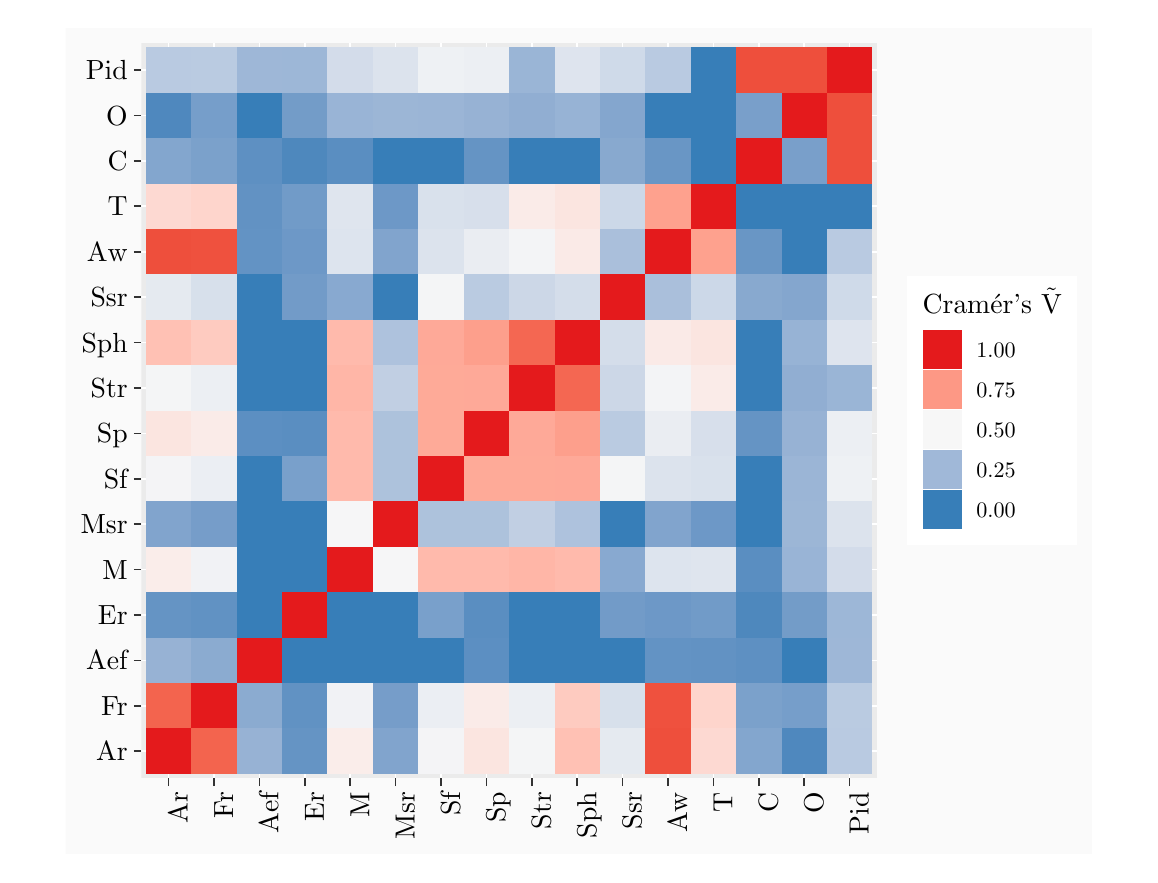
\begin{tikzpicture}[x=1pt,y=1pt]
\definecolor{fillColor}{RGB}{255,255,255}
\path[use as bounding box,fill=fillColor,fill opacity=0.00] (0,0) rectangle (398.34,298.75);
\begin{scope}
\path[clip] ( 13.60,  0.00) rectangle (384.73,298.75);
\definecolor{drawColor}{RGB}{255,255,255}
\definecolor{fillColor}{gray}{0.98}

\path[draw=drawColor,line width= 0.6pt,line join=round,line cap=round,fill=fillColor] ( 13.60,  0.00) rectangle (384.73,298.75);
\end{scope}
\begin{scope}
\path[clip] ( 41.08, 27.47) rectangle (306.86,293.25);
\definecolor{fillColor}{gray}{0.92}

\path[fill=fillColor] ( 41.08, 27.47) rectangle (306.86,293.25);
\definecolor{drawColor}{RGB}{255,255,255}

\path[draw=drawColor,line width= 0.6pt,line join=round] ( 41.08, 37.32) --
	(306.86, 37.32);

\path[draw=drawColor,line width= 0.6pt,line join=round] ( 41.08, 53.72) --
	(306.86, 53.72);

\path[draw=drawColor,line width= 0.6pt,line join=round] ( 41.08, 70.13) --
	(306.86, 70.13);

\path[draw=drawColor,line width= 0.6pt,line join=round] ( 41.08, 86.54) --
	(306.86, 86.54);

\path[draw=drawColor,line width= 0.6pt,line join=round] ( 41.08,102.94) --
	(306.86,102.94);

\path[draw=drawColor,line width= 0.6pt,line join=round] ( 41.08,119.35) --
	(306.86,119.35);

\path[draw=drawColor,line width= 0.6pt,line join=round] ( 41.08,135.75) --
	(306.86,135.75);

\path[draw=drawColor,line width= 0.6pt,line join=round] ( 41.08,152.16) --
	(306.86,152.16);

\path[draw=drawColor,line width= 0.6pt,line join=round] ( 41.08,168.57) --
	(306.86,168.57);

\path[draw=drawColor,line width= 0.6pt,line join=round] ( 41.08,184.97) --
	(306.86,184.97);

\path[draw=drawColor,line width= 0.6pt,line join=round] ( 41.08,201.38) --
	(306.86,201.38);

\path[draw=drawColor,line width= 0.6pt,line join=round] ( 41.08,217.79) --
	(306.86,217.79);

\path[draw=drawColor,line width= 0.6pt,line join=round] ( 41.08,234.19) --
	(306.86,234.19);

\path[draw=drawColor,line width= 0.6pt,line join=round] ( 41.08,250.60) --
	(306.86,250.60);

\path[draw=drawColor,line width= 0.6pt,line join=round] ( 41.08,267.00) --
	(306.86,267.00);

\path[draw=drawColor,line width= 0.6pt,line join=round] ( 41.08,283.41) --
	(306.86,283.41);

\path[draw=drawColor,line width= 0.6pt,line join=round] ( 50.92, 27.47) --
	( 50.92,293.25);

\path[draw=drawColor,line width= 0.6pt,line join=round] ( 67.33, 27.47) --
	( 67.33,293.25);

\path[draw=drawColor,line width= 0.6pt,line join=round] ( 83.73, 27.47) --
	( 83.73,293.25);

\path[draw=drawColor,line width= 0.6pt,line join=round] (100.14, 27.47) --
	(100.14,293.25);

\path[draw=drawColor,line width= 0.6pt,line join=round] (116.55, 27.47) --
	(116.55,293.25);

\path[draw=drawColor,line width= 0.6pt,line join=round] (132.95, 27.47) --
	(132.95,293.25);

\path[draw=drawColor,line width= 0.6pt,line join=round] (149.36, 27.47) --
	(149.36,293.25);

\path[draw=drawColor,line width= 0.6pt,line join=round] (165.76, 27.47) --
	(165.76,293.25);

\path[draw=drawColor,line width= 0.6pt,line join=round] (182.17, 27.47) --
	(182.17,293.25);

\path[draw=drawColor,line width= 0.6pt,line join=round] (198.58, 27.47) --
	(198.58,293.25);

\path[draw=drawColor,line width= 0.6pt,line join=round] (214.98, 27.47) --
	(214.98,293.25);

\path[draw=drawColor,line width= 0.6pt,line join=round] (231.39, 27.47) --
	(231.39,293.25);

\path[draw=drawColor,line width= 0.6pt,line join=round] (247.80, 27.47) --
	(247.80,293.25);

\path[draw=drawColor,line width= 0.6pt,line join=round] (264.20, 27.47) --
	(264.20,293.25);

\path[draw=drawColor,line width= 0.6pt,line join=round] (280.61, 27.47) --
	(280.61,293.25);

\path[draw=drawColor,line width= 0.6pt,line join=round] (297.01, 27.47) --
	(297.01,293.25);
\definecolor{fillColor}{RGB}{228,26,28}

\path[fill=fillColor] ( 42.72, 29.11) rectangle ( 59.12, 45.52);
\definecolor{fillColor}{RGB}{243,100,78}

\path[fill=fillColor] ( 59.12, 29.11) rectangle ( 75.53, 45.52);
\definecolor{fillColor}{RGB}{151,178,212}

\path[fill=fillColor] ( 75.53, 29.11) rectangle ( 91.94, 45.52);
\definecolor{fillColor}{RGB}{101,148,196}

\path[fill=fillColor] ( 91.94, 29.11) rectangle (108.34, 45.52);
\definecolor{fillColor}{RGB}{250,237,234}

\path[fill=fillColor] (108.34, 29.11) rectangle (124.75, 45.52);
\definecolor{fillColor}{RGB}{129,164,205}

\path[fill=fillColor] (124.75, 29.11) rectangle (141.16, 45.52);
\definecolor{fillColor}{RGB}{244,244,246}

\path[fill=fillColor] (141.16, 29.11) rectangle (157.56, 45.52);
\definecolor{fillColor}{RGB}{251,229,224}

\path[fill=fillColor] (157.56, 29.11) rectangle (173.97, 45.52);
\definecolor{fillColor}{RGB}{244,245,246}

\path[fill=fillColor] (173.97, 29.11) rectangle (190.37, 45.52);
\definecolor{fillColor}{RGB}{255,193,180}

\path[fill=fillColor] (190.37, 29.11) rectangle (206.78, 45.52);
\definecolor{fillColor}{RGB}{229,234,240}

\path[fill=fillColor] (206.78, 29.11) rectangle (223.19, 45.52);
\definecolor{fillColor}{RGB}{238,79,60}

\path[fill=fillColor] (223.19, 29.11) rectangle (239.59, 45.52);
\definecolor{fillColor}{RGB}{253,217,210}

\path[fill=fillColor] (239.59, 29.11) rectangle (256.00, 45.52);
\definecolor{fillColor}{RGB}{131,166,206}

\path[fill=fillColor] (256.00, 29.11) rectangle (272.40, 45.52);
\definecolor{fillColor}{RGB}{79,136,190}

\path[fill=fillColor] (272.40, 29.11) rectangle (288.81, 45.52);
\definecolor{fillColor}{RGB}{185,202,225}

\path[fill=fillColor] (288.81, 29.11) rectangle (305.22, 45.52);
\definecolor{fillColor}{RGB}{243,100,78}

\path[fill=fillColor] ( 42.72, 45.52) rectangle ( 59.12, 61.93);
\definecolor{fillColor}{RGB}{228,26,28}

\path[fill=fillColor] ( 59.12, 45.52) rectangle ( 75.53, 61.93);
\definecolor{fillColor}{RGB}{139,171,208}

\path[fill=fillColor] ( 75.53, 45.52) rectangle ( 91.94, 61.93);
\definecolor{fillColor}{RGB}{97,146,195}

\path[fill=fillColor] ( 91.94, 45.52) rectangle (108.34, 61.93);
\definecolor{fillColor}{RGB}{241,242,245}

\path[fill=fillColor] (108.34, 45.52) rectangle (124.75, 61.93);
\definecolor{fillColor}{RGB}{118,157,201}

\path[fill=fillColor] (124.75, 45.52) rectangle (141.16, 61.93);
\definecolor{fillColor}{RGB}{235,238,243}

\path[fill=fillColor] (141.16, 45.52) rectangle (157.56, 61.93);
\definecolor{fillColor}{RGB}{250,235,232}

\path[fill=fillColor] (157.56, 45.52) rectangle (173.97, 61.93);
\definecolor{fillColor}{RGB}{236,239,243}

\path[fill=fillColor] (173.97, 45.52) rectangle (190.37, 61.93);
\definecolor{fillColor}{RGB}{254,203,192}

\path[fill=fillColor] (190.37, 45.52) rectangle (206.78, 61.93);
\definecolor{fillColor}{RGB}{215,224,235}

\path[fill=fillColor] (206.78, 45.52) rectangle (223.19, 61.93);
\definecolor{fillColor}{RGB}{239,81,62}

\path[fill=fillColor] (223.19, 45.52) rectangle (239.59, 61.93);
\definecolor{fillColor}{RGB}{254,213,204}

\path[fill=fillColor] (239.59, 45.52) rectangle (256.00, 61.93);
\definecolor{fillColor}{RGB}{123,161,203}

\path[fill=fillColor] (256.00, 45.52) rectangle (272.40, 61.93);
\definecolor{fillColor}{RGB}{118,158,202}

\path[fill=fillColor] (272.40, 45.52) rectangle (288.81, 61.93);
\definecolor{fillColor}{RGB}{186,203,225}

\path[fill=fillColor] (288.81, 45.52) rectangle (305.22, 61.93);
\definecolor{fillColor}{RGB}{151,178,212}

\path[fill=fillColor] ( 42.72, 61.93) rectangle ( 59.12, 78.33);
\definecolor{fillColor}{RGB}{139,171,208}

\path[fill=fillColor] ( 59.12, 61.93) rectangle ( 75.53, 78.33);
\definecolor{fillColor}{RGB}{228,26,28}

\path[fill=fillColor] ( 75.53, 61.93) rectangle ( 91.94, 78.33);
\definecolor{fillColor}{RGB}{55,126,184}

\path[fill=fillColor] ( 91.94, 61.93) rectangle (108.34, 78.33);

\path[fill=fillColor] (108.34, 61.93) rectangle (124.75, 78.33);

\path[fill=fillColor] (124.75, 61.93) rectangle (141.16, 78.33);

\path[fill=fillColor] (141.16, 61.93) rectangle (157.56, 78.33);
\definecolor{fillColor}{RGB}{92,143,194}

\path[fill=fillColor] (157.56, 61.93) rectangle (173.97, 78.33);
\definecolor{fillColor}{RGB}{55,126,184}

\path[fill=fillColor] (173.97, 61.93) rectangle (190.37, 78.33);

\path[fill=fillColor] (190.37, 61.93) rectangle (206.78, 78.33);

\path[fill=fillColor] (206.78, 61.93) rectangle (223.19, 78.33);
\definecolor{fillColor}{RGB}{99,147,196}

\path[fill=fillColor] (223.19, 61.93) rectangle (239.59, 78.33);
\definecolor{fillColor}{RGB}{98,146,195}

\path[fill=fillColor] (239.59, 61.93) rectangle (256.00, 78.33);
\definecolor{fillColor}{RGB}{94,144,194}

\path[fill=fillColor] (256.00, 61.93) rectangle (272.40, 78.33);
\definecolor{fillColor}{RGB}{55,126,184}

\path[fill=fillColor] (272.40, 61.93) rectangle (288.81, 78.33);
\definecolor{fillColor}{RGB}{158,183,215}

\path[fill=fillColor] (288.81, 61.93) rectangle (305.22, 78.33);
\definecolor{fillColor}{RGB}{101,148,196}

\path[fill=fillColor] ( 42.72, 78.33) rectangle ( 59.12, 94.74);
\definecolor{fillColor}{RGB}{97,146,195}

\path[fill=fillColor] ( 59.12, 78.33) rectangle ( 75.53, 94.74);
\definecolor{fillColor}{RGB}{55,126,184}

\path[fill=fillColor] ( 75.53, 78.33) rectangle ( 91.94, 94.74);
\definecolor{fillColor}{RGB}{228,26,28}

\path[fill=fillColor] ( 91.94, 78.33) rectangle (108.34, 94.74);
\definecolor{fillColor}{RGB}{55,126,184}

\path[fill=fillColor] (108.34, 78.33) rectangle (124.75, 94.74);

\path[fill=fillColor] (124.75, 78.33) rectangle (141.16, 94.74);
\definecolor{fillColor}{RGB}{121,160,203}

\path[fill=fillColor] (141.16, 78.33) rectangle (157.56, 94.74);
\definecolor{fillColor}{RGB}{90,142,193}

\path[fill=fillColor] (157.56, 78.33) rectangle (173.97, 94.74);
\definecolor{fillColor}{RGB}{55,126,184}

\path[fill=fillColor] (173.97, 78.33) rectangle (190.37, 94.74);

\path[fill=fillColor] (190.37, 78.33) rectangle (206.78, 94.74);
\definecolor{fillColor}{RGB}{114,155,200}

\path[fill=fillColor] (206.78, 78.33) rectangle (223.19, 94.74);
\definecolor{fillColor}{RGB}{109,152,199}

\path[fill=fillColor] (223.19, 78.33) rectangle (239.59, 94.74);
\definecolor{fillColor}{RGB}{113,155,200}

\path[fill=fillColor] (239.59, 78.33) rectangle (256.00, 94.74);
\definecolor{fillColor}{RGB}{78,136,189}

\path[fill=fillColor] (256.00, 78.33) rectangle (272.40, 94.74);
\definecolor{fillColor}{RGB}{115,156,200}

\path[fill=fillColor] (272.40, 78.33) rectangle (288.81, 94.74);
\definecolor{fillColor}{RGB}{157,183,215}

\path[fill=fillColor] (288.81, 78.33) rectangle (305.22, 94.74);
\definecolor{fillColor}{RGB}{250,237,234}

\path[fill=fillColor] ( 42.72, 94.74) rectangle ( 59.12,111.15);
\definecolor{fillColor}{RGB}{241,242,245}

\path[fill=fillColor] ( 59.12, 94.74) rectangle ( 75.53,111.15);
\definecolor{fillColor}{RGB}{55,126,184}

\path[fill=fillColor] ( 75.53, 94.74) rectangle ( 91.94,111.15);

\path[fill=fillColor] ( 91.94, 94.74) rectangle (108.34,111.15);
\definecolor{fillColor}{RGB}{228,26,28}

\path[fill=fillColor] (108.34, 94.74) rectangle (124.75,111.15);
\definecolor{fillColor}{RGB}{246,246,247}

\path[fill=fillColor] (124.75, 94.74) rectangle (141.16,111.15);
\definecolor{fillColor}{RGB}{255,186,172}

\path[fill=fillColor] (141.16, 94.74) rectangle (157.56,111.15);

\path[fill=fillColor] (157.56, 94.74) rectangle (173.97,111.15);
\definecolor{fillColor}{RGB}{255,182,167}

\path[fill=fillColor] (173.97, 94.74) rectangle (190.37,111.15);
\definecolor{fillColor}{RGB}{255,186,172}

\path[fill=fillColor] (190.37, 94.74) rectangle (206.78,111.15);
\definecolor{fillColor}{RGB}{136,169,208}

\path[fill=fillColor] (206.78, 94.74) rectangle (223.19,111.15);
\definecolor{fillColor}{RGB}{221,228,238}

\path[fill=fillColor] (223.19, 94.74) rectangle (239.59,111.15);
\definecolor{fillColor}{RGB}{223,229,238}

\path[fill=fillColor] (239.59, 94.74) rectangle (256.00,111.15);
\definecolor{fillColor}{RGB}{90,142,193}

\path[fill=fillColor] (256.00, 94.74) rectangle (272.40,111.15);
\definecolor{fillColor}{RGB}{153,180,214}

\path[fill=fillColor] (272.40, 94.74) rectangle (288.81,111.15);
\definecolor{fillColor}{RGB}{211,220,234}

\path[fill=fillColor] (288.81, 94.74) rectangle (305.22,111.15);
\definecolor{fillColor}{RGB}{129,164,205}

\path[fill=fillColor] ( 42.72,111.15) rectangle ( 59.12,127.55);
\definecolor{fillColor}{RGB}{118,157,201}

\path[fill=fillColor] ( 59.12,111.15) rectangle ( 75.53,127.55);
\definecolor{fillColor}{RGB}{55,126,184}

\path[fill=fillColor] ( 75.53,111.15) rectangle ( 91.94,127.55);

\path[fill=fillColor] ( 91.94,111.15) rectangle (108.34,127.55);
\definecolor{fillColor}{RGB}{246,246,247}

\path[fill=fillColor] (108.34,111.15) rectangle (124.75,127.55);
\definecolor{fillColor}{RGB}{228,26,28}

\path[fill=fillColor] (124.75,111.15) rectangle (141.16,127.55);
\definecolor{fillColor}{RGB}{173,194,220}

\path[fill=fillColor] (141.16,111.15) rectangle (157.56,127.55);

\path[fill=fillColor] (157.56,111.15) rectangle (173.97,127.55);
\definecolor{fillColor}{RGB}{193,207,227}

\path[fill=fillColor] (173.97,111.15) rectangle (190.37,127.55);
\definecolor{fillColor}{RGB}{174,194,221}

\path[fill=fillColor] (190.37,111.15) rectangle (206.78,127.55);
\definecolor{fillColor}{RGB}{55,126,184}

\path[fill=fillColor] (206.78,111.15) rectangle (223.19,127.55);
\definecolor{fillColor}{RGB}{129,164,205}

\path[fill=fillColor] (223.19,111.15) rectangle (239.59,127.55);
\definecolor{fillColor}{RGB}{109,152,199}

\path[fill=fillColor] (239.59,111.15) rectangle (256.00,127.55);
\definecolor{fillColor}{RGB}{55,126,184}

\path[fill=fillColor] (256.00,111.15) rectangle (272.40,127.55);
\definecolor{fillColor}{RGB}{156,182,214}

\path[fill=fillColor] (272.40,111.15) rectangle (288.81,127.55);
\definecolor{fillColor}{RGB}{220,227,237}

\path[fill=fillColor] (288.81,111.15) rectangle (305.22,127.55);
\definecolor{fillColor}{RGB}{244,244,246}

\path[fill=fillColor] ( 42.72,127.55) rectangle ( 59.12,143.96);
\definecolor{fillColor}{RGB}{235,238,243}

\path[fill=fillColor] ( 59.12,127.55) rectangle ( 75.53,143.96);
\definecolor{fillColor}{RGB}{55,126,184}

\path[fill=fillColor] ( 75.53,127.55) rectangle ( 91.94,143.96);
\definecolor{fillColor}{RGB}{121,160,203}

\path[fill=fillColor] ( 91.94,127.55) rectangle (108.34,143.96);
\definecolor{fillColor}{RGB}{255,186,172}

\path[fill=fillColor] (108.34,127.55) rectangle (124.75,143.96);
\definecolor{fillColor}{RGB}{173,194,220}

\path[fill=fillColor] (124.75,127.55) rectangle (141.16,143.96);
\definecolor{fillColor}{RGB}{228,26,28}

\path[fill=fillColor] (141.16,127.55) rectangle (157.56,143.96);
\definecolor{fillColor}{RGB}{254,170,152}

\path[fill=fillColor] (157.56,127.55) rectangle (173.97,143.96);

\path[fill=fillColor] (173.97,127.55) rectangle (190.37,143.96);
\definecolor{fillColor}{RGB}{254,169,152}

\path[fill=fillColor] (190.37,127.55) rectangle (206.78,143.96);
\definecolor{fillColor}{RGB}{244,245,246}

\path[fill=fillColor] (206.78,127.55) rectangle (223.19,143.96);
\definecolor{fillColor}{RGB}{220,227,237}

\path[fill=fillColor] (223.19,127.55) rectangle (239.59,143.96);
\definecolor{fillColor}{RGB}{217,225,236}

\path[fill=fillColor] (239.59,127.55) rectangle (256.00,143.96);
\definecolor{fillColor}{RGB}{55,126,184}

\path[fill=fillColor] (256.00,127.55) rectangle (272.40,143.96);
\definecolor{fillColor}{RGB}{155,181,214}

\path[fill=fillColor] (272.40,127.55) rectangle (288.81,143.96);
\definecolor{fillColor}{RGB}{238,241,244}

\path[fill=fillColor] (288.81,127.55) rectangle (305.22,143.96);
\definecolor{fillColor}{RGB}{251,229,224}

\path[fill=fillColor] ( 42.72,143.96) rectangle ( 59.12,160.36);
\definecolor{fillColor}{RGB}{250,235,232}

\path[fill=fillColor] ( 59.12,143.96) rectangle ( 75.53,160.36);
\definecolor{fillColor}{RGB}{92,143,194}

\path[fill=fillColor] ( 75.53,143.96) rectangle ( 91.94,160.36);
\definecolor{fillColor}{RGB}{90,142,193}

\path[fill=fillColor] ( 91.94,143.96) rectangle (108.34,160.36);
\definecolor{fillColor}{RGB}{255,186,172}

\path[fill=fillColor] (108.34,143.96) rectangle (124.75,160.36);
\definecolor{fillColor}{RGB}{173,194,220}

\path[fill=fillColor] (124.75,143.96) rectangle (141.16,160.36);
\definecolor{fillColor}{RGB}{254,170,152}

\path[fill=fillColor] (141.16,143.96) rectangle (157.56,160.36);
\definecolor{fillColor}{RGB}{228,26,28}

\path[fill=fillColor] (157.56,143.96) rectangle (173.97,160.36);
\definecolor{fillColor}{RGB}{254,169,152}

\path[fill=fillColor] (173.97,143.96) rectangle (190.37,160.36);
\definecolor{fillColor}{RGB}{253,159,140}

\path[fill=fillColor] (190.37,143.96) rectangle (206.78,160.36);
\definecolor{fillColor}{RGB}{186,203,225}

\path[fill=fillColor] (206.78,143.96) rectangle (223.19,160.36);
\definecolor{fillColor}{RGB}{234,237,242}

\path[fill=fillColor] (223.19,143.96) rectangle (239.59,160.36);
\definecolor{fillColor}{RGB}{215,223,235}

\path[fill=fillColor] (239.59,143.96) rectangle (256.00,160.36);
\definecolor{fillColor}{RGB}{101,148,196}

\path[fill=fillColor] (256.00,143.96) rectangle (272.40,160.36);
\definecolor{fillColor}{RGB}{151,178,212}

\path[fill=fillColor] (272.40,143.96) rectangle (288.81,160.36);
\definecolor{fillColor}{RGB}{236,239,243}

\path[fill=fillColor] (288.81,143.96) rectangle (305.22,160.36);
\definecolor{fillColor}{RGB}{244,245,246}

\path[fill=fillColor] ( 42.72,160.36) rectangle ( 59.12,176.77);
\definecolor{fillColor}{RGB}{236,239,243}

\path[fill=fillColor] ( 59.12,160.36) rectangle ( 75.53,176.77);
\definecolor{fillColor}{RGB}{55,126,184}

\path[fill=fillColor] ( 75.53,160.36) rectangle ( 91.94,176.77);

\path[fill=fillColor] ( 91.94,160.36) rectangle (108.34,176.77);
\definecolor{fillColor}{RGB}{255,182,167}

\path[fill=fillColor] (108.34,160.36) rectangle (124.75,176.77);
\definecolor{fillColor}{RGB}{193,207,227}

\path[fill=fillColor] (124.75,160.36) rectangle (141.16,176.77);
\definecolor{fillColor}{RGB}{254,170,152}

\path[fill=fillColor] (141.16,160.36) rectangle (157.56,176.77);
\definecolor{fillColor}{RGB}{254,169,152}

\path[fill=fillColor] (157.56,160.36) rectangle (173.97,176.77);
\definecolor{fillColor}{RGB}{228,26,28}

\path[fill=fillColor] (173.97,160.36) rectangle (190.37,176.77);
\definecolor{fillColor}{RGB}{244,103,82}

\path[fill=fillColor] (190.37,160.36) rectangle (206.78,176.77);
\definecolor{fillColor}{RGB}{204,215,231}

\path[fill=fillColor] (206.78,160.36) rectangle (223.19,176.77);
\definecolor{fillColor}{RGB}{243,244,246}

\path[fill=fillColor] (223.19,160.36) rectangle (239.59,176.77);
\definecolor{fillColor}{RGB}{250,235,232}

\path[fill=fillColor] (239.59,160.36) rectangle (256.00,176.77);
\definecolor{fillColor}{RGB}{55,126,184}

\path[fill=fillColor] (256.00,160.36) rectangle (272.40,176.77);
\definecolor{fillColor}{RGB}{145,174,210}

\path[fill=fillColor] (272.40,160.36) rectangle (288.81,176.77);
\definecolor{fillColor}{RGB}{154,181,214}

\path[fill=fillColor] (288.81,160.36) rectangle (305.22,176.77);
\definecolor{fillColor}{RGB}{255,193,180}

\path[fill=fillColor] ( 42.72,176.77) rectangle ( 59.12,193.18);
\definecolor{fillColor}{RGB}{254,203,192}

\path[fill=fillColor] ( 59.12,176.77) rectangle ( 75.53,193.18);
\definecolor{fillColor}{RGB}{55,126,184}

\path[fill=fillColor] ( 75.53,176.77) rectangle ( 91.94,193.18);

\path[fill=fillColor] ( 91.94,176.77) rectangle (108.34,193.18);
\definecolor{fillColor}{RGB}{255,186,172}

\path[fill=fillColor] (108.34,176.77) rectangle (124.75,193.18);
\definecolor{fillColor}{RGB}{174,194,221}

\path[fill=fillColor] (124.75,176.77) rectangle (141.16,193.18);
\definecolor{fillColor}{RGB}{254,169,152}

\path[fill=fillColor] (141.16,176.77) rectangle (157.56,193.18);
\definecolor{fillColor}{RGB}{253,159,140}

\path[fill=fillColor] (157.56,176.77) rectangle (173.97,193.18);
\definecolor{fillColor}{RGB}{244,103,82}

\path[fill=fillColor] (173.97,176.77) rectangle (190.37,193.18);
\definecolor{fillColor}{RGB}{228,26,28}

\path[fill=fillColor] (190.37,176.77) rectangle (206.78,193.18);
\definecolor{fillColor}{RGB}{212,221,234}

\path[fill=fillColor] (206.78,176.77) rectangle (223.19,193.18);
\definecolor{fillColor}{RGB}{250,234,231}

\path[fill=fillColor] (223.19,176.77) rectangle (239.59,193.18);
\definecolor{fillColor}{RGB}{251,229,224}

\path[fill=fillColor] (239.59,176.77) rectangle (256.00,193.18);
\definecolor{fillColor}{RGB}{55,126,184}

\path[fill=fillColor] (256.00,176.77) rectangle (272.40,193.18);
\definecolor{fillColor}{RGB}{151,179,213}

\path[fill=fillColor] (272.40,176.77) rectangle (288.81,193.18);
\definecolor{fillColor}{RGB}{222,228,238}

\path[fill=fillColor] (288.81,176.77) rectangle (305.22,193.18);
\definecolor{fillColor}{RGB}{229,234,240}

\path[fill=fillColor] ( 42.72,193.18) rectangle ( 59.12,209.58);
\definecolor{fillColor}{RGB}{215,224,235}

\path[fill=fillColor] ( 59.12,193.18) rectangle ( 75.53,209.58);
\definecolor{fillColor}{RGB}{55,126,184}

\path[fill=fillColor] ( 75.53,193.18) rectangle ( 91.94,209.58);
\definecolor{fillColor}{RGB}{114,155,200}

\path[fill=fillColor] ( 91.94,193.18) rectangle (108.34,209.58);
\definecolor{fillColor}{RGB}{136,169,208}

\path[fill=fillColor] (108.34,193.18) rectangle (124.75,209.58);
\definecolor{fillColor}{RGB}{55,126,184}

\path[fill=fillColor] (124.75,193.18) rectangle (141.16,209.58);
\definecolor{fillColor}{RGB}{244,245,246}

\path[fill=fillColor] (141.16,193.18) rectangle (157.56,209.58);
\definecolor{fillColor}{RGB}{186,203,225}

\path[fill=fillColor] (157.56,193.18) rectangle (173.97,209.58);
\definecolor{fillColor}{RGB}{204,215,231}

\path[fill=fillColor] (173.97,193.18) rectangle (190.37,209.58);
\definecolor{fillColor}{RGB}{212,221,234}

\path[fill=fillColor] (190.37,193.18) rectangle (206.78,209.58);
\definecolor{fillColor}{RGB}{228,26,28}

\path[fill=fillColor] (206.78,193.18) rectangle (223.19,209.58);
\definecolor{fillColor}{RGB}{170,191,219}

\path[fill=fillColor] (223.19,193.18) rectangle (239.59,209.58);
\definecolor{fillColor}{RGB}{204,216,232}

\path[fill=fillColor] (239.59,193.18) rectangle (256.00,209.58);
\definecolor{fillColor}{RGB}{136,169,207}

\path[fill=fillColor] (256.00,193.18) rectangle (272.40,209.58);
\definecolor{fillColor}{RGB}{132,166,206}

\path[fill=fillColor] (272.40,193.18) rectangle (288.81,209.58);
\definecolor{fillColor}{RGB}{207,218,233}

\path[fill=fillColor] (288.81,193.18) rectangle (305.22,209.58);
\definecolor{fillColor}{RGB}{238,79,60}

\path[fill=fillColor] ( 42.72,209.58) rectangle ( 59.12,225.99);
\definecolor{fillColor}{RGB}{239,81,62}

\path[fill=fillColor] ( 59.12,209.58) rectangle ( 75.53,225.99);
\definecolor{fillColor}{RGB}{99,147,196}

\path[fill=fillColor] ( 75.53,209.58) rectangle ( 91.94,225.99);
\definecolor{fillColor}{RGB}{109,152,199}

\path[fill=fillColor] ( 91.94,209.58) rectangle (108.34,225.99);
\definecolor{fillColor}{RGB}{221,228,238}

\path[fill=fillColor] (108.34,209.58) rectangle (124.75,225.99);
\definecolor{fillColor}{RGB}{129,164,205}

\path[fill=fillColor] (124.75,209.58) rectangle (141.16,225.99);
\definecolor{fillColor}{RGB}{220,227,237}

\path[fill=fillColor] (141.16,209.58) rectangle (157.56,225.99);
\definecolor{fillColor}{RGB}{234,237,242}

\path[fill=fillColor] (157.56,209.58) rectangle (173.97,225.99);
\definecolor{fillColor}{RGB}{243,244,246}

\path[fill=fillColor] (173.97,209.58) rectangle (190.37,225.99);
\definecolor{fillColor}{RGB}{250,234,231}

\path[fill=fillColor] (190.37,209.58) rectangle (206.78,225.99);
\definecolor{fillColor}{RGB}{170,191,219}

\path[fill=fillColor] (206.78,209.58) rectangle (223.19,225.99);
\definecolor{fillColor}{RGB}{228,26,28}

\path[fill=fillColor] (223.19,209.58) rectangle (239.59,225.99);
\definecolor{fillColor}{RGB}{254,161,142}

\path[fill=fillColor] (239.59,209.58) rectangle (256.00,225.99);
\definecolor{fillColor}{RGB}{105,150,197}

\path[fill=fillColor] (256.00,209.58) rectangle (272.40,225.99);
\definecolor{fillColor}{RGB}{55,126,184}

\path[fill=fillColor] (272.40,209.58) rectangle (288.81,225.99);
\definecolor{fillColor}{RGB}{185,202,225}

\path[fill=fillColor] (288.81,209.58) rectangle (305.22,225.99);
\definecolor{fillColor}{RGB}{253,217,210}

\path[fill=fillColor] ( 42.72,225.99) rectangle ( 59.12,242.39);
\definecolor{fillColor}{RGB}{254,213,204}

\path[fill=fillColor] ( 59.12,225.99) rectangle ( 75.53,242.39);
\definecolor{fillColor}{RGB}{98,146,195}

\path[fill=fillColor] ( 75.53,225.99) rectangle ( 91.94,242.39);
\definecolor{fillColor}{RGB}{113,155,200}

\path[fill=fillColor] ( 91.94,225.99) rectangle (108.34,242.39);
\definecolor{fillColor}{RGB}{223,229,238}

\path[fill=fillColor] (108.34,225.99) rectangle (124.75,242.39);
\definecolor{fillColor}{RGB}{109,152,199}

\path[fill=fillColor] (124.75,225.99) rectangle (141.16,242.39);
\definecolor{fillColor}{RGB}{217,225,236}

\path[fill=fillColor] (141.16,225.99) rectangle (157.56,242.39);
\definecolor{fillColor}{RGB}{215,223,235}

\path[fill=fillColor] (157.56,225.99) rectangle (173.97,242.39);
\definecolor{fillColor}{RGB}{250,235,232}

\path[fill=fillColor] (173.97,225.99) rectangle (190.37,242.39);
\definecolor{fillColor}{RGB}{251,229,224}

\path[fill=fillColor] (190.37,225.99) rectangle (206.78,242.39);
\definecolor{fillColor}{RGB}{204,216,232}

\path[fill=fillColor] (206.78,225.99) rectangle (223.19,242.39);
\definecolor{fillColor}{RGB}{254,161,142}

\path[fill=fillColor] (223.19,225.99) rectangle (239.59,242.39);
\definecolor{fillColor}{RGB}{228,26,28}

\path[fill=fillColor] (239.59,225.99) rectangle (256.00,242.39);
\definecolor{fillColor}{RGB}{55,126,184}

\path[fill=fillColor] (256.00,225.99) rectangle (272.40,242.39);

\path[fill=fillColor] (272.40,225.99) rectangle (288.81,242.39);

\path[fill=fillColor] (288.81,225.99) rectangle (305.22,242.39);
\definecolor{fillColor}{RGB}{131,166,206}

\path[fill=fillColor] ( 42.72,242.39) rectangle ( 59.12,258.80);
\definecolor{fillColor}{RGB}{123,161,203}

\path[fill=fillColor] ( 59.12,242.39) rectangle ( 75.53,258.80);
\definecolor{fillColor}{RGB}{94,144,194}

\path[fill=fillColor] ( 75.53,242.39) rectangle ( 91.94,258.80);
\definecolor{fillColor}{RGB}{78,136,189}

\path[fill=fillColor] ( 91.94,242.39) rectangle (108.34,258.80);
\definecolor{fillColor}{RGB}{90,142,193}

\path[fill=fillColor] (108.34,242.39) rectangle (124.75,258.80);
\definecolor{fillColor}{RGB}{55,126,184}

\path[fill=fillColor] (124.75,242.39) rectangle (141.16,258.80);

\path[fill=fillColor] (141.16,242.39) rectangle (157.56,258.80);
\definecolor{fillColor}{RGB}{101,148,196}

\path[fill=fillColor] (157.56,242.39) rectangle (173.97,258.80);
\definecolor{fillColor}{RGB}{55,126,184}

\path[fill=fillColor] (173.97,242.39) rectangle (190.37,258.80);

\path[fill=fillColor] (190.37,242.39) rectangle (206.78,258.80);
\definecolor{fillColor}{RGB}{136,169,207}

\path[fill=fillColor] (206.78,242.39) rectangle (223.19,258.80);
\definecolor{fillColor}{RGB}{105,150,197}

\path[fill=fillColor] (223.19,242.39) rectangle (239.59,258.80);
\definecolor{fillColor}{RGB}{55,126,184}

\path[fill=fillColor] (239.59,242.39) rectangle (256.00,258.80);
\definecolor{fillColor}{RGB}{228,26,28}

\path[fill=fillColor] (256.00,242.39) rectangle (272.40,258.80);
\definecolor{fillColor}{RGB}{121,159,202}

\path[fill=fillColor] (272.40,242.39) rectangle (288.81,258.80);
\definecolor{fillColor}{RGB}{238,79,60}

\path[fill=fillColor] (288.81,242.39) rectangle (305.22,258.80);
\definecolor{fillColor}{RGB}{79,136,190}

\path[fill=fillColor] ( 42.72,258.80) rectangle ( 59.12,275.21);
\definecolor{fillColor}{RGB}{118,158,202}

\path[fill=fillColor] ( 59.12,258.80) rectangle ( 75.53,275.21);
\definecolor{fillColor}{RGB}{55,126,184}

\path[fill=fillColor] ( 75.53,258.80) rectangle ( 91.94,275.21);
\definecolor{fillColor}{RGB}{115,156,200}

\path[fill=fillColor] ( 91.94,258.80) rectangle (108.34,275.21);
\definecolor{fillColor}{RGB}{153,180,214}

\path[fill=fillColor] (108.34,258.80) rectangle (124.75,275.21);
\definecolor{fillColor}{RGB}{156,182,214}

\path[fill=fillColor] (124.75,258.80) rectangle (141.16,275.21);
\definecolor{fillColor}{RGB}{155,181,214}

\path[fill=fillColor] (141.16,258.80) rectangle (157.56,275.21);
\definecolor{fillColor}{RGB}{151,178,212}

\path[fill=fillColor] (157.56,258.80) rectangle (173.97,275.21);
\definecolor{fillColor}{RGB}{145,174,210}

\path[fill=fillColor] (173.97,258.80) rectangle (190.37,275.21);
\definecolor{fillColor}{RGB}{151,179,213}

\path[fill=fillColor] (190.37,258.80) rectangle (206.78,275.21);
\definecolor{fillColor}{RGB}{132,166,206}

\path[fill=fillColor] (206.78,258.80) rectangle (223.19,275.21);
\definecolor{fillColor}{RGB}{55,126,184}

\path[fill=fillColor] (223.19,258.80) rectangle (239.59,275.21);

\path[fill=fillColor] (239.59,258.80) rectangle (256.00,275.21);
\definecolor{fillColor}{RGB}{121,159,202}

\path[fill=fillColor] (256.00,258.80) rectangle (272.40,275.21);
\definecolor{fillColor}{RGB}{228,26,28}

\path[fill=fillColor] (272.40,258.80) rectangle (288.81,275.21);
\definecolor{fillColor}{RGB}{238,79,60}

\path[fill=fillColor] (288.81,258.80) rectangle (305.22,275.21);
\definecolor{fillColor}{RGB}{185,202,225}

\path[fill=fillColor] ( 42.72,275.21) rectangle ( 59.12,291.61);
\definecolor{fillColor}{RGB}{186,203,225}

\path[fill=fillColor] ( 59.12,275.21) rectangle ( 75.53,291.61);
\definecolor{fillColor}{RGB}{158,183,215}

\path[fill=fillColor] ( 75.53,275.21) rectangle ( 91.94,291.61);
\definecolor{fillColor}{RGB}{157,183,215}

\path[fill=fillColor] ( 91.94,275.21) rectangle (108.34,291.61);
\definecolor{fillColor}{RGB}{211,220,234}

\path[fill=fillColor] (108.34,275.21) rectangle (124.75,291.61);
\definecolor{fillColor}{RGB}{220,227,237}

\path[fill=fillColor] (124.75,275.21) rectangle (141.16,291.61);
\definecolor{fillColor}{RGB}{238,241,244}

\path[fill=fillColor] (141.16,275.21) rectangle (157.56,291.61);
\definecolor{fillColor}{RGB}{236,239,243}

\path[fill=fillColor] (157.56,275.21) rectangle (173.97,291.61);
\definecolor{fillColor}{RGB}{154,181,214}

\path[fill=fillColor] (173.97,275.21) rectangle (190.37,291.61);
\definecolor{fillColor}{RGB}{222,228,238}

\path[fill=fillColor] (190.37,275.21) rectangle (206.78,291.61);
\definecolor{fillColor}{RGB}{207,218,233}

\path[fill=fillColor] (206.78,275.21) rectangle (223.19,291.61);
\definecolor{fillColor}{RGB}{185,202,225}

\path[fill=fillColor] (223.19,275.21) rectangle (239.59,291.61);
\definecolor{fillColor}{RGB}{55,126,184}

\path[fill=fillColor] (239.59,275.21) rectangle (256.00,291.61);
\definecolor{fillColor}{RGB}{238,79,60}

\path[fill=fillColor] (256.00,275.21) rectangle (272.40,291.61);

\path[fill=fillColor] (272.40,275.21) rectangle (288.81,291.61);
\definecolor{fillColor}{RGB}{228,26,28}

\path[fill=fillColor] (288.81,275.21) rectangle (305.22,291.61);
\end{scope}
\begin{scope}
\path[clip] (  0.00,  0.00) rectangle (398.34,298.75);
\definecolor{drawColor}{RGB}{0,0,0}

\node[text=drawColor,anchor=base east,inner sep=0pt, outer sep=0pt, scale=  1.00] at ( 36.13, 33.87) {Ar};

\node[text=drawColor,anchor=base east,inner sep=0pt, outer sep=0pt, scale=  1.00] at ( 36.13, 50.28) {Fr};

\node[text=drawColor,anchor=base east,inner sep=0pt, outer sep=0pt, scale=  1.00] at ( 36.13, 66.69) {Aef};

\node[text=drawColor,anchor=base east,inner sep=0pt, outer sep=0pt, scale=  1.00] at ( 36.13, 83.09) {Er};

\node[text=drawColor,anchor=base east,inner sep=0pt, outer sep=0pt, scale=  1.00] at ( 36.13, 99.50) {M};

\node[text=drawColor,anchor=base east,inner sep=0pt, outer sep=0pt, scale=  1.00] at ( 36.13,115.90) {Msr};

\node[text=drawColor,anchor=base east,inner sep=0pt, outer sep=0pt, scale=  1.00] at ( 36.13,132.31) {Sf};

\node[text=drawColor,anchor=base east,inner sep=0pt, outer sep=0pt, scale=  1.00] at ( 36.13,148.72) {Sp};

\node[text=drawColor,anchor=base east,inner sep=0pt, outer sep=0pt, scale=  1.00] at ( 36.13,165.12) {Str};

\node[text=drawColor,anchor=base east,inner sep=0pt, outer sep=0pt, scale=  1.00] at ( 36.13,181.53) {Sph};

\node[text=drawColor,anchor=base east,inner sep=0pt, outer sep=0pt, scale=  1.00] at ( 36.13,197.94) {Ssr};

\node[text=drawColor,anchor=base east,inner sep=0pt, outer sep=0pt, scale=  1.00] at ( 36.13,214.34) {Aw};

\node[text=drawColor,anchor=base east,inner sep=0pt, outer sep=0pt, scale=  1.00] at ( 36.13,230.75) {T};

\node[text=drawColor,anchor=base east,inner sep=0pt, outer sep=0pt, scale=  1.00] at ( 36.13,247.15) {C};

\node[text=drawColor,anchor=base east,inner sep=0pt, outer sep=0pt, scale=  1.00] at ( 36.13,263.56) {O};

\node[text=drawColor,anchor=base east,inner sep=0pt, outer sep=0pt, scale=  1.00] at ( 36.13,279.97) {Pid};
\end{scope}
\begin{scope}
\path[clip] (  0.00,  0.00) rectangle (398.34,298.75);
\definecolor{drawColor}{gray}{0.20}

\path[draw=drawColor,line width= 0.6pt,line join=round] ( 38.33, 37.32) --
	( 41.08, 37.32);

\path[draw=drawColor,line width= 0.6pt,line join=round] ( 38.33, 53.72) --
	( 41.08, 53.72);

\path[draw=drawColor,line width= 0.6pt,line join=round] ( 38.33, 70.13) --
	( 41.08, 70.13);

\path[draw=drawColor,line width= 0.6pt,line join=round] ( 38.33, 86.54) --
	( 41.08, 86.54);

\path[draw=drawColor,line width= 0.6pt,line join=round] ( 38.33,102.94) --
	( 41.08,102.94);

\path[draw=drawColor,line width= 0.6pt,line join=round] ( 38.33,119.35) --
	( 41.08,119.35);

\path[draw=drawColor,line width= 0.6pt,line join=round] ( 38.33,135.75) --
	( 41.08,135.75);

\path[draw=drawColor,line width= 0.6pt,line join=round] ( 38.33,152.16) --
	( 41.08,152.16);

\path[draw=drawColor,line width= 0.6pt,line join=round] ( 38.33,168.57) --
	( 41.08,168.57);

\path[draw=drawColor,line width= 0.6pt,line join=round] ( 38.33,184.97) --
	( 41.08,184.97);

\path[draw=drawColor,line width= 0.6pt,line join=round] ( 38.33,201.38) --
	( 41.08,201.38);

\path[draw=drawColor,line width= 0.6pt,line join=round] ( 38.33,217.79) --
	( 41.08,217.79);

\path[draw=drawColor,line width= 0.6pt,line join=round] ( 38.33,234.19) --
	( 41.08,234.19);

\path[draw=drawColor,line width= 0.6pt,line join=round] ( 38.33,250.60) --
	( 41.08,250.60);

\path[draw=drawColor,line width= 0.6pt,line join=round] ( 38.33,267.00) --
	( 41.08,267.00);

\path[draw=drawColor,line width= 0.6pt,line join=round] ( 38.33,283.41) --
	( 41.08,283.41);
\end{scope}
\begin{scope}
\path[clip] (  0.00,  0.00) rectangle (398.34,298.75);
\definecolor{drawColor}{gray}{0.20}

\path[draw=drawColor,line width= 0.6pt,line join=round] ( 50.92, 24.72) --
	( 50.92, 27.47);

\path[draw=drawColor,line width= 0.6pt,line join=round] ( 67.33, 24.72) --
	( 67.33, 27.47);

\path[draw=drawColor,line width= 0.6pt,line join=round] ( 83.73, 24.72) --
	( 83.73, 27.47);

\path[draw=drawColor,line width= 0.6pt,line join=round] (100.14, 24.72) --
	(100.14, 27.47);

\path[draw=drawColor,line width= 0.6pt,line join=round] (116.55, 24.72) --
	(116.55, 27.47);

\path[draw=drawColor,line width= 0.6pt,line join=round] (132.95, 24.72) --
	(132.95, 27.47);

\path[draw=drawColor,line width= 0.6pt,line join=round] (149.36, 24.72) --
	(149.36, 27.47);

\path[draw=drawColor,line width= 0.6pt,line join=round] (165.76, 24.72) --
	(165.76, 27.47);

\path[draw=drawColor,line width= 0.6pt,line join=round] (182.17, 24.72) --
	(182.17, 27.47);

\path[draw=drawColor,line width= 0.6pt,line join=round] (198.58, 24.72) --
	(198.58, 27.47);

\path[draw=drawColor,line width= 0.6pt,line join=round] (214.98, 24.72) --
	(214.98, 27.47);

\path[draw=drawColor,line width= 0.6pt,line join=round] (231.39, 24.72) --
	(231.39, 27.47);

\path[draw=drawColor,line width= 0.6pt,line join=round] (247.80, 24.72) --
	(247.80, 27.47);

\path[draw=drawColor,line width= 0.6pt,line join=round] (264.20, 24.72) --
	(264.20, 27.47);

\path[draw=drawColor,line width= 0.6pt,line join=round] (280.61, 24.72) --
	(280.61, 27.47);

\path[draw=drawColor,line width= 0.6pt,line join=round] (297.01, 24.72) --
	(297.01, 27.47);
\end{scope}
\begin{scope}
\path[clip] (  0.00,  0.00) rectangle (398.34,298.75);
\definecolor{drawColor}{RGB}{0,0,0}

\node[text=drawColor,rotate= 90.00,anchor=base east,inner sep=0pt, outer sep=0pt, scale=  1.00] at ( 57.81, 22.52) {Ar};

\node[text=drawColor,rotate= 90.00,anchor=base east,inner sep=0pt, outer sep=0pt, scale=  1.00] at ( 74.21, 22.52) {Fr};

\node[text=drawColor,rotate= 90.00,anchor=base east,inner sep=0pt, outer sep=0pt, scale=  1.00] at ( 90.62, 22.52) {Aef};

\node[text=drawColor,rotate= 90.00,anchor=base east,inner sep=0pt, outer sep=0pt, scale=  1.00] at (107.03, 22.52) {Er};

\node[text=drawColor,rotate= 90.00,anchor=base east,inner sep=0pt, outer sep=0pt, scale=  1.00] at (123.43, 22.52) {M};

\node[text=drawColor,rotate= 90.00,anchor=base east,inner sep=0pt, outer sep=0pt, scale=  1.00] at (139.84, 22.52) {Msr};

\node[text=drawColor,rotate= 90.00,anchor=base east,inner sep=0pt, outer sep=0pt, scale=  1.00] at (156.25, 22.52) {Sf};

\node[text=drawColor,rotate= 90.00,anchor=base east,inner sep=0pt, outer sep=0pt, scale=  1.00] at (172.65, 22.52) {Sp};

\node[text=drawColor,rotate= 90.00,anchor=base east,inner sep=0pt, outer sep=0pt, scale=  1.00] at (189.06, 22.52) {Str};

\node[text=drawColor,rotate= 90.00,anchor=base east,inner sep=0pt, outer sep=0pt, scale=  1.00] at (205.46, 22.52) {Sph};

\node[text=drawColor,rotate= 90.00,anchor=base east,inner sep=0pt, outer sep=0pt, scale=  1.00] at (221.87, 22.52) {Ssr};

\node[text=drawColor,rotate= 90.00,anchor=base east,inner sep=0pt, outer sep=0pt, scale=  1.00] at (238.28, 22.52) {Aw};

\node[text=drawColor,rotate= 90.00,anchor=base east,inner sep=0pt, outer sep=0pt, scale=  1.00] at (254.68, 22.52) {T};

\node[text=drawColor,rotate= 90.00,anchor=base east,inner sep=0pt, outer sep=0pt, scale=  1.00] at (271.09, 22.52) {C};

\node[text=drawColor,rotate= 90.00,anchor=base east,inner sep=0pt, outer sep=0pt, scale=  1.00] at (287.50, 22.52) {O};

\node[text=drawColor,rotate= 90.00,anchor=base east,inner sep=0pt, outer sep=0pt, scale=  1.00] at (303.90, 22.52) {Pid};
\end{scope}
\begin{scope}
\path[clip] (  0.00,  0.00) rectangle (398.34,298.75);
\definecolor{fillColor}{RGB}{255,255,255}

\path[fill=fillColor] (317.86,111.81) rectangle (379.23,208.91);
\end{scope}
\begin{scope}
\path[clip] (  0.00,  0.00) rectangle (398.34,298.75);
\definecolor{drawColor}{RGB}{0,0,0}

\node[text=drawColor,anchor=base west,inner sep=0pt, outer sep=0pt, scale=  1.00] at (323.36,195.56) {Cram\'er's \~V};
\end{scope}
\begin{scope}
\path[clip] (  0.00,  0.00) rectangle (398.34,298.75);
\definecolor{drawColor}{RGB}{255,255,255}
\definecolor{fillColor}{gray}{0.95}

\path[draw=drawColor,line width= 0.6pt,line join=round,line cap=round,fill=fillColor] (323.36,175.13) rectangle (337.81,189.58);
\end{scope}
\begin{scope}
\path[clip] (  0.00,  0.00) rectangle (398.34,298.75);
\definecolor{fillColor}{RGB}{228,26,28}

\path[fill=fillColor] (323.50,175.27) rectangle (337.67,189.44);
\end{scope}
\begin{scope}
\path[clip] (  0.00,  0.00) rectangle (398.34,298.75);
\definecolor{drawColor}{RGB}{255,255,255}
\definecolor{fillColor}{gray}{0.95}

\path[draw=drawColor,line width= 0.6pt,line join=round,line cap=round,fill=fillColor] (323.36,160.68) rectangle (337.81,175.13);
\end{scope}
\begin{scope}
\path[clip] (  0.00,  0.00) rectangle (398.34,298.75);
\definecolor{fillColor}{RGB}{253,152,133}

\path[fill=fillColor] (323.50,160.82) rectangle (337.67,174.99);
\end{scope}
\begin{scope}
\path[clip] (  0.00,  0.00) rectangle (398.34,298.75);
\definecolor{drawColor}{RGB}{255,255,255}
\definecolor{fillColor}{gray}{0.95}

\path[draw=drawColor,line width= 0.6pt,line join=round,line cap=round,fill=fillColor] (323.36,146.22) rectangle (337.81,160.68);
\end{scope}
\begin{scope}
\path[clip] (  0.00,  0.00) rectangle (398.34,298.75);
\definecolor{fillColor}{gray}{0.97}

\path[fill=fillColor] (323.50,146.36) rectangle (337.67,160.53);
\end{scope}
\begin{scope}
\path[clip] (  0.00,  0.00) rectangle (398.34,298.75);
\definecolor{drawColor}{RGB}{255,255,255}
\definecolor{fillColor}{gray}{0.95}

\path[draw=drawColor,line width= 0.6pt,line join=round,line cap=round,fill=fillColor] (323.36,131.77) rectangle (337.81,146.22);
\end{scope}
\begin{scope}
\path[clip] (  0.00,  0.00) rectangle (398.34,298.75);
\definecolor{fillColor}{RGB}{160,184,216}

\path[fill=fillColor] (323.50,131.91) rectangle (337.67,146.08);
\end{scope}
\begin{scope}
\path[clip] (  0.00,  0.00) rectangle (398.34,298.75);
\definecolor{drawColor}{RGB}{255,255,255}
\definecolor{fillColor}{gray}{0.95}

\path[draw=drawColor,line width= 0.6pt,line join=round,line cap=round,fill=fillColor] (323.36,117.31) rectangle (337.81,131.77);
\end{scope}
\begin{scope}
\path[clip] (  0.00,  0.00) rectangle (398.34,298.75);
\definecolor{fillColor}{RGB}{55,126,184}

\path[fill=fillColor] (323.50,117.46) rectangle (337.67,131.62);
\end{scope}
\begin{scope}
\path[clip] (  0.00,  0.00) rectangle (398.34,298.75);
\definecolor{drawColor}{RGB}{0,0,0}

\node[text=drawColor,anchor=base west,inner sep=0pt, outer sep=0pt, scale=  0.80] at (342.81,179.60) {1.00};
\end{scope}
\begin{scope}
\path[clip] (  0.00,  0.00) rectangle (398.34,298.75);
\definecolor{drawColor}{RGB}{0,0,0}

\node[text=drawColor,anchor=base west,inner sep=0pt, outer sep=0pt, scale=  0.80] at (342.81,165.15) {0.75};
\end{scope}
\begin{scope}
\path[clip] (  0.00,  0.00) rectangle (398.34,298.75);
\definecolor{drawColor}{RGB}{0,0,0}

\node[text=drawColor,anchor=base west,inner sep=0pt, outer sep=0pt, scale=  0.80] at (342.81,150.69) {0.50};
\end{scope}
\begin{scope}
\path[clip] (  0.00,  0.00) rectangle (398.34,298.75);
\definecolor{drawColor}{RGB}{0,0,0}

\node[text=drawColor,anchor=base west,inner sep=0pt, outer sep=0pt, scale=  0.80] at (342.81,136.24) {0.25};
\end{scope}
\begin{scope}
\path[clip] (  0.00,  0.00) rectangle (398.34,298.75);
\definecolor{drawColor}{RGB}{0,0,0}

\node[text=drawColor,anchor=base west,inner sep=0pt, outer sep=0pt, scale=  0.80] at (342.81,121.79) {0.00};
\end{scope}
\end{tikzpicture}

            }
          };}
          \action<4->{\node (a) at (.25\textwidth,-.55\textwidth)
          {
            \resizebox{.5\textwidth}{!}{%
              % Created by tikzDevice version 0.12
% !TEX encoding = UTF-8 Unicode
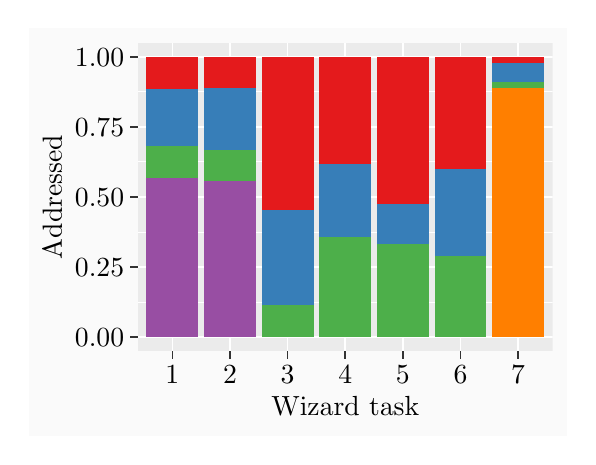
\begin{tikzpicture}[x=1pt,y=1pt]
\definecolor{fillColor}{RGB}{255,255,255}
\path[use as bounding box,fill=fillColor,fill opacity=0.00] (0,0) rectangle (195.19,147.70);
\begin{scope}
\path[clip] (  0.00,  0.00) rectangle (195.19,147.70);
\definecolor{drawColor}{RGB}{255,255,255}
\definecolor{fillColor}{gray}{0.98}

\path[draw=drawColor,line width= 0.6pt,line join=round,line cap=round,fill=fillColor] (  0.00,  0.00) rectangle (195.19,147.70);
\end{scope}
\begin{scope}
\path[clip] ( 39.80, 30.86) rectangle (189.69,142.20);
\definecolor{fillColor}{gray}{0.92}

\path[fill=fillColor] ( 39.80, 30.86) rectangle (189.69,142.20);
\definecolor{drawColor}{RGB}{255,255,255}

\path[draw=drawColor,line width= 0.3pt,line join=round] ( 39.80, 48.58) --
	(189.69, 48.58);

\path[draw=drawColor,line width= 0.3pt,line join=round] ( 39.80, 73.88) --
	(189.69, 73.88);

\path[draw=drawColor,line width= 0.3pt,line join=round] ( 39.80, 99.19) --
	(189.69, 99.19);

\path[draw=drawColor,line width= 0.3pt,line join=round] ( 39.80,124.49) --
	(189.69,124.49);

\path[draw=drawColor,line width= 0.6pt,line join=round] ( 39.80, 35.92) --
	(189.69, 35.92);

\path[draw=drawColor,line width= 0.6pt,line join=round] ( 39.80, 61.23) --
	(189.69, 61.23);

\path[draw=drawColor,line width= 0.6pt,line join=round] ( 39.80, 86.53) --
	(189.69, 86.53);

\path[draw=drawColor,line width= 0.6pt,line join=round] ( 39.80,111.84) --
	(189.69,111.84);

\path[draw=drawColor,line width= 0.6pt,line join=round] ( 39.80,137.14) --
	(189.69,137.14);

\path[draw=drawColor,line width= 0.6pt,line join=round] ( 52.29, 30.86) --
	( 52.29,142.20);

\path[draw=drawColor,line width= 0.6pt,line join=round] ( 73.11, 30.86) --
	( 73.11,142.20);

\path[draw=drawColor,line width= 0.6pt,line join=round] ( 93.93, 30.86) --
	( 93.93,142.20);

\path[draw=drawColor,line width= 0.6pt,line join=round] (114.75, 30.86) --
	(114.75,142.20);

\path[draw=drawColor,line width= 0.6pt,line join=round] (135.56, 30.86) --
	(135.56,142.20);

\path[draw=drawColor,line width= 0.6pt,line join=round] (156.38, 30.86) --
	(156.38,142.20);

\path[draw=drawColor,line width= 0.6pt,line join=round] (177.20, 30.86) --
	(177.20,142.20);
\definecolor{fillColor}{RGB}{152,78,163}

\path[fill=fillColor] ( 42.93, 35.92) rectangle ( 61.66, 93.43);
\definecolor{fillColor}{RGB}{77,175,74}

\path[fill=fillColor] ( 42.93, 93.43) rectangle ( 61.66,104.94);
\definecolor{fillColor}{RGB}{55,126,184}

\path[fill=fillColor] ( 42.93,104.94) rectangle ( 61.66,125.64);
\definecolor{fillColor}{RGB}{228,26,28}

\path[fill=fillColor] ( 42.93,125.64) rectangle ( 61.66,137.14);
\definecolor{fillColor}{RGB}{152,78,163}

\path[fill=fillColor] ( 63.74, 35.92) rectangle ( 82.48, 92.16);
\definecolor{fillColor}{RGB}{77,175,74}

\path[fill=fillColor] ( 63.74, 92.16) rectangle ( 82.48,103.40);
\definecolor{fillColor}{RGB}{55,126,184}

\path[fill=fillColor] ( 63.74,103.40) rectangle ( 82.48,125.90);
\definecolor{fillColor}{RGB}{228,26,28}

\path[fill=fillColor] ( 63.74,125.90) rectangle ( 82.48,137.14);
\definecolor{fillColor}{RGB}{77,175,74}

\path[fill=fillColor] ( 84.56, 35.92) rectangle (103.30, 47.43);
\definecolor{fillColor}{RGB}{55,126,184}

\path[fill=fillColor] ( 84.56, 47.43) rectangle (103.30, 81.93);
\definecolor{fillColor}{RGB}{228,26,28}

\path[fill=fillColor] ( 84.56, 81.93) rectangle (103.30,137.14);
\definecolor{fillColor}{RGB}{77,175,74}

\path[fill=fillColor] (105.38, 35.92) rectangle (124.11, 72.07);
\definecolor{fillColor}{RGB}{55,126,184}

\path[fill=fillColor] (105.38, 72.07) rectangle (124.11, 98.58);
\definecolor{fillColor}{RGB}{228,26,28}

\path[fill=fillColor] (105.38, 98.58) rectangle (124.11,137.14);
\definecolor{fillColor}{RGB}{77,175,74}

\path[fill=fillColor] (126.19, 35.92) rectangle (144.93, 69.66);
\definecolor{fillColor}{RGB}{55,126,184}

\path[fill=fillColor] (126.19, 69.66) rectangle (144.93, 84.12);
\definecolor{fillColor}{RGB}{228,26,28}

\path[fill=fillColor] (126.19, 84.12) rectangle (144.93,137.14);
\definecolor{fillColor}{RGB}{77,175,74}

\path[fill=fillColor] (147.01, 35.92) rectangle (165.75, 65.16);
\definecolor{fillColor}{RGB}{55,126,184}

\path[fill=fillColor] (147.01, 65.16) rectangle (165.75, 96.66);
\definecolor{fillColor}{RGB}{228,26,28}

\path[fill=fillColor] (147.01, 96.66) rectangle (165.75,137.14);
\definecolor{fillColor}{RGB}{255,127,0}

\path[fill=fillColor] (167.83, 35.92) rectangle (186.56,125.90);
\definecolor{fillColor}{RGB}{77,175,74}

\path[fill=fillColor] (167.83,125.90) rectangle (186.56,128.15);
\definecolor{fillColor}{RGB}{55,126,184}

\path[fill=fillColor] (167.83,128.15) rectangle (186.56,134.89);
\definecolor{fillColor}{RGB}{228,26,28}

\path[fill=fillColor] (167.83,134.89) rectangle (186.56,137.14);
\end{scope}
\begin{scope}
\path[clip] (  0.00,  0.00) rectangle (195.19,147.70);
\definecolor{drawColor}{RGB}{0,0,0}

\node[text=drawColor,anchor=base east,inner sep=0pt, outer sep=0pt, scale=  1.00] at ( 34.85, 32.48) {0.00};

\node[text=drawColor,anchor=base east,inner sep=0pt, outer sep=0pt, scale=  1.00] at ( 34.85, 57.78) {0.25};

\node[text=drawColor,anchor=base east,inner sep=0pt, outer sep=0pt, scale=  1.00] at ( 34.85, 83.09) {0.50};

\node[text=drawColor,anchor=base east,inner sep=0pt, outer sep=0pt, scale=  1.00] at ( 34.85,108.39) {0.75};

\node[text=drawColor,anchor=base east,inner sep=0pt, outer sep=0pt, scale=  1.00] at ( 34.85,133.70) {1.00};
\end{scope}
\begin{scope}
\path[clip] (  0.00,  0.00) rectangle (195.19,147.70);
\definecolor{drawColor}{gray}{0.20}

\path[draw=drawColor,line width= 0.6pt,line join=round] ( 37.05, 35.92) --
	( 39.80, 35.92);

\path[draw=drawColor,line width= 0.6pt,line join=round] ( 37.05, 61.23) --
	( 39.80, 61.23);

\path[draw=drawColor,line width= 0.6pt,line join=round] ( 37.05, 86.53) --
	( 39.80, 86.53);

\path[draw=drawColor,line width= 0.6pt,line join=round] ( 37.05,111.84) --
	( 39.80,111.84);

\path[draw=drawColor,line width= 0.6pt,line join=round] ( 37.05,137.14) --
	( 39.80,137.14);
\end{scope}
\begin{scope}
\path[clip] (  0.00,  0.00) rectangle (195.19,147.70);
\definecolor{drawColor}{gray}{0.20}

\path[draw=drawColor,line width= 0.6pt,line join=round] ( 52.29, 28.11) --
	( 52.29, 30.86);

\path[draw=drawColor,line width= 0.6pt,line join=round] ( 73.11, 28.11) --
	( 73.11, 30.86);

\path[draw=drawColor,line width= 0.6pt,line join=round] ( 93.93, 28.11) --
	( 93.93, 30.86);

\path[draw=drawColor,line width= 0.6pt,line join=round] (114.75, 28.11) --
	(114.75, 30.86);

\path[draw=drawColor,line width= 0.6pt,line join=round] (135.56, 28.11) --
	(135.56, 30.86);

\path[draw=drawColor,line width= 0.6pt,line join=round] (156.38, 28.11) --
	(156.38, 30.86);

\path[draw=drawColor,line width= 0.6pt,line join=round] (177.20, 28.11) --
	(177.20, 30.86);
\end{scope}
\begin{scope}
\path[clip] (  0.00,  0.00) rectangle (195.19,147.70);
\definecolor{drawColor}{RGB}{0,0,0}

\node[text=drawColor,anchor=base,inner sep=0pt, outer sep=0pt, scale=  1.00] at ( 52.29, 19.03) {1};

\node[text=drawColor,anchor=base,inner sep=0pt, outer sep=0pt, scale=  1.00] at ( 73.11, 19.03) {2};

\node[text=drawColor,anchor=base,inner sep=0pt, outer sep=0pt, scale=  1.00] at ( 93.93, 19.03) {3};

\node[text=drawColor,anchor=base,inner sep=0pt, outer sep=0pt, scale=  1.00] at (114.75, 19.03) {4};

\node[text=drawColor,anchor=base,inner sep=0pt, outer sep=0pt, scale=  1.00] at (135.56, 19.03) {5};

\node[text=drawColor,anchor=base,inner sep=0pt, outer sep=0pt, scale=  1.00] at (156.38, 19.03) {6};

\node[text=drawColor,anchor=base,inner sep=0pt, outer sep=0pt, scale=  1.00] at (177.20, 19.03) {7};
\end{scope}
\begin{scope}
\path[clip] (  0.00,  0.00) rectangle (195.19,147.70);
\definecolor{drawColor}{RGB}{0,0,0}

\node[text=drawColor,anchor=base,inner sep=0pt, outer sep=0pt, scale=  1.00] at (114.75,  7.44) {Wizard task};
\end{scope}
\begin{scope}
\path[clip] (  0.00,  0.00) rectangle (195.19,147.70);
\definecolor{drawColor}{RGB}{0,0,0}

\node[text=drawColor,rotate= 90.00,anchor=base,inner sep=0pt, outer sep=0pt, scale=  1.00] at ( 12.39, 86.53) {Addressed};
\end{scope}
\end{tikzpicture}

            }
          };}
          \action<3->{\node (a) at (-.25\textwidth,-.55\textwidth)
          {
            \resizebox{.5\textwidth}{!}{%
              % Created by tikzDevice version 0.12
% !TEX encoding = UTF-8 Unicode
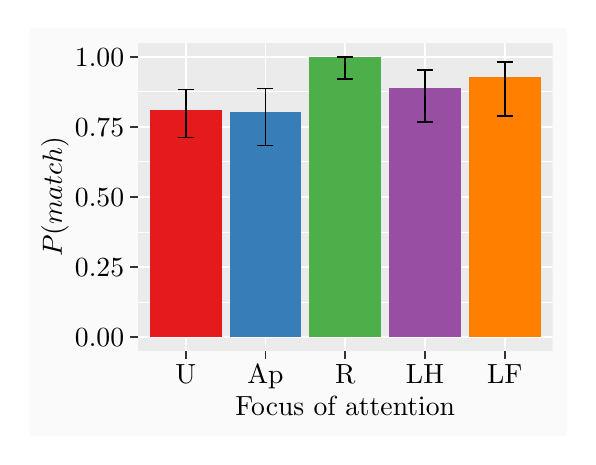
\begin{tikzpicture}[x=1pt,y=1pt]
\definecolor{fillColor}{RGB}{255,255,255}
\path[use as bounding box,fill=fillColor,fill opacity=0.00] (0,0) rectangle (195.19,147.70);
\begin{scope}
\path[clip] (  0.00,  0.00) rectangle (195.19,147.70);
\definecolor{drawColor}{RGB}{255,255,255}
\definecolor{fillColor}{gray}{0.98}

\path[draw=drawColor,line width= 0.6pt,line join=round,line cap=round,fill=fillColor] (  0.00,  0.00) rectangle (195.19,147.70);
\end{scope}
\begin{scope}
\path[clip] ( 39.80, 30.86) rectangle (189.69,142.20);
\definecolor{fillColor}{gray}{0.92}

\path[fill=fillColor] ( 39.80, 30.86) rectangle (189.69,142.20);
\definecolor{drawColor}{RGB}{255,255,255}

\path[draw=drawColor,line width= 0.3pt,line join=round] ( 39.80, 48.58) --
	(189.69, 48.58);

\path[draw=drawColor,line width= 0.3pt,line join=round] ( 39.80, 73.88) --
	(189.69, 73.88);

\path[draw=drawColor,line width= 0.3pt,line join=round] ( 39.80, 99.19) --
	(189.69, 99.19);

\path[draw=drawColor,line width= 0.3pt,line join=round] ( 39.80,124.49) --
	(189.69,124.49);

\path[draw=drawColor,line width= 0.6pt,line join=round] ( 39.80, 35.92) --
	(189.69, 35.92);

\path[draw=drawColor,line width= 0.6pt,line join=round] ( 39.80, 61.23) --
	(189.69, 61.23);

\path[draw=drawColor,line width= 0.6pt,line join=round] ( 39.80, 86.53) --
	(189.69, 86.53);

\path[draw=drawColor,line width= 0.6pt,line join=round] ( 39.80,111.84) --
	(189.69,111.84);

\path[draw=drawColor,line width= 0.6pt,line join=round] ( 39.80,137.14) --
	(189.69,137.14);

\path[draw=drawColor,line width= 0.6pt,line join=round] ( 57.10, 30.86) --
	( 57.10,142.20);

\path[draw=drawColor,line width= 0.6pt,line join=round] ( 85.92, 30.86) --
	( 85.92,142.20);

\path[draw=drawColor,line width= 0.6pt,line join=round] (114.75, 30.86) --
	(114.75,142.20);

\path[draw=drawColor,line width= 0.6pt,line join=round] (143.57, 30.86) --
	(143.57,142.20);

\path[draw=drawColor,line width= 0.6pt,line join=round] (172.39, 30.86) --
	(172.39,142.20);
\definecolor{fillColor}{RGB}{228,26,28}

\path[fill=fillColor] ( 44.13, 35.92) rectangle ( 70.07,118.02);
\definecolor{fillColor}{RGB}{55,126,184}

\path[fill=fillColor] ( 72.95, 35.92) rectangle ( 98.89,117.21);
\definecolor{fillColor}{RGB}{77,175,74}

\path[fill=fillColor] (101.77, 35.92) rectangle (127.72,137.14);
\definecolor{fillColor}{RGB}{152,78,163}

\path[fill=fillColor] (130.60, 35.92) rectangle (156.54,125.90);
\definecolor{fillColor}{RGB}{255,127,0}

\path[fill=fillColor] (159.42, 35.92) rectangle (185.36,129.74);
\definecolor{drawColor}{RGB}{0,0,0}

\path[draw=drawColor,line width= 0.6pt,line join=round] ( 54.22,125.31) --
	( 59.98,125.31);

\path[draw=drawColor,line width= 0.6pt,line join=round] ( 57.10,125.31) --
	( 57.10,107.99);

\path[draw=drawColor,line width= 0.6pt,line join=round] ( 54.22,107.99) --
	( 59.98,107.99);

\path[draw=drawColor,line width= 0.6pt,line join=round] ( 83.04,125.70) --
	( 88.80,125.70);

\path[draw=drawColor,line width= 0.6pt,line join=round] ( 85.92,125.70) --
	( 85.92,105.08);

\path[draw=drawColor,line width= 0.6pt,line join=round] ( 83.04,105.08) --
	( 88.80,105.08);

\path[draw=drawColor,line width= 0.6pt,line join=round] (111.86,137.14) --
	(117.63,137.14);

\path[draw=drawColor,line width= 0.6pt,line join=round] (114.75,137.14) --
	(114.75,129.05);

\path[draw=drawColor,line width= 0.6pt,line join=round] (111.86,129.05) --
	(117.63,129.05);

\path[draw=drawColor,line width= 0.6pt,line join=round] (140.69,132.49) --
	(146.45,132.49);

\path[draw=drawColor,line width= 0.6pt,line join=round] (143.57,132.49) --
	(143.57,113.54);

\path[draw=drawColor,line width= 0.6pt,line join=round] (140.69,113.54) --
	(146.45,113.54);

\path[draw=drawColor,line width= 0.6pt,line join=round] (169.51,135.21) --
	(175.27,135.21);

\path[draw=drawColor,line width= 0.6pt,line join=round] (172.39,135.21) --
	(172.39,115.88);

\path[draw=drawColor,line width= 0.6pt,line join=round] (169.51,115.88) --
	(175.27,115.88);
\end{scope}
\begin{scope}
\path[clip] (  0.00,  0.00) rectangle (195.19,147.70);
\definecolor{drawColor}{RGB}{0,0,0}

\node[text=drawColor,anchor=base east,inner sep=0pt, outer sep=0pt, scale=  1.00] at ( 34.85, 32.48) {0.00};

\node[text=drawColor,anchor=base east,inner sep=0pt, outer sep=0pt, scale=  1.00] at ( 34.85, 57.78) {0.25};

\node[text=drawColor,anchor=base east,inner sep=0pt, outer sep=0pt, scale=  1.00] at ( 34.85, 83.09) {0.50};

\node[text=drawColor,anchor=base east,inner sep=0pt, outer sep=0pt, scale=  1.00] at ( 34.85,108.39) {0.75};

\node[text=drawColor,anchor=base east,inner sep=0pt, outer sep=0pt, scale=  1.00] at ( 34.85,133.70) {1.00};
\end{scope}
\begin{scope}
\path[clip] (  0.00,  0.00) rectangle (195.19,147.70);
\definecolor{drawColor}{gray}{0.20}

\path[draw=drawColor,line width= 0.6pt,line join=round] ( 37.05, 35.92) --
	( 39.80, 35.92);

\path[draw=drawColor,line width= 0.6pt,line join=round] ( 37.05, 61.23) --
	( 39.80, 61.23);

\path[draw=drawColor,line width= 0.6pt,line join=round] ( 37.05, 86.53) --
	( 39.80, 86.53);

\path[draw=drawColor,line width= 0.6pt,line join=round] ( 37.05,111.84) --
	( 39.80,111.84);

\path[draw=drawColor,line width= 0.6pt,line join=round] ( 37.05,137.14) --
	( 39.80,137.14);
\end{scope}
\begin{scope}
\path[clip] (  0.00,  0.00) rectangle (195.19,147.70);
\definecolor{drawColor}{gray}{0.20}

\path[draw=drawColor,line width= 0.6pt,line join=round] ( 57.10, 28.11) --
	( 57.10, 30.86);

\path[draw=drawColor,line width= 0.6pt,line join=round] ( 85.92, 28.11) --
	( 85.92, 30.86);

\path[draw=drawColor,line width= 0.6pt,line join=round] (114.75, 28.11) --
	(114.75, 30.86);

\path[draw=drawColor,line width= 0.6pt,line join=round] (143.57, 28.11) --
	(143.57, 30.86);

\path[draw=drawColor,line width= 0.6pt,line join=round] (172.39, 28.11) --
	(172.39, 30.86);
\end{scope}
\begin{scope}
\path[clip] (  0.00,  0.00) rectangle (195.19,147.70);
\definecolor{drawColor}{RGB}{0,0,0}

\node[text=drawColor,anchor=base,inner sep=0pt, outer sep=0pt, scale=  1.00] at ( 57.10, 19.03) {U};

\node[text=drawColor,anchor=base,inner sep=0pt, outer sep=0pt, scale=  1.00] at ( 85.92, 19.03) {Ap};

\node[text=drawColor,anchor=base,inner sep=0pt, outer sep=0pt, scale=  1.00] at (114.75, 19.03) {R};

\node[text=drawColor,anchor=base,inner sep=0pt, outer sep=0pt, scale=  1.00] at (143.57, 19.03) {LH};

\node[text=drawColor,anchor=base,inner sep=0pt, outer sep=0pt, scale=  1.00] at (172.39, 19.03) {LF};
\end{scope}
\begin{scope}
\path[clip] (  0.00,  0.00) rectangle (195.19,147.70);
\definecolor{drawColor}{RGB}{0,0,0}

\node[text=drawColor,anchor=base,inner sep=0pt, outer sep=0pt, scale=  1.00] at (114.75,  7.44) {Focus of attention};
\end{scope}
\begin{scope}
\path[clip] (  0.00,  0.00) rectangle (195.19,147.70);
\definecolor{drawColor}{RGB}{0,0,0}

\node[text=drawColor,rotate= 90.00,anchor=base,inner sep=0pt, outer sep=0pt, scale=  1.00] at ( 12.39, 86.53) {\(P(match)\)};
\end{scope}
\end{tikzpicture}

            }
          };}
         \end{tikzpicture}
       }
    \end{column}
    \hspace{-.1\textwidth}
    \begin{column}{.6\textwidth}
      \begin{itemize}
        \item<1-> Pearson: Overall strong correlations
        \item<2-> Cramer V: Strongest association for Fr, Aw, T, M, S*
        \item<3-> Addressee mostly equals the focus of attention
        \item<4-> Addressee distribution is task dependant
      \end{itemize}
    \end{column}
  \end{columns}
\end{frame}
\begin{frame}{Addressing Apartment Variables --- Other}
  \begin{description}
      \item[{Wizard \gls{addressee} [Aw]:}] Encodes which entity is chosen by the \gls{wizard} to react to a communication attempt.
      It can take the values \emph{Apartment}, \emph{Floor lamp}, or \emph{Robot}.
      \item[{Wizard task [T]:}] Tells which task is solved in a specific observation.
      \item[{Condition [C]:}] Encodes whether the participant is in the verbal or non-verbal condition.
      \item[{Order [O]:}] tells whether the tasks were be solved in normal or alternative order.
      \item[{Participant Id [Pid]:}] Numerically identifies the participant.
  \end{description}
\end{frame}
\begin{frame}{Addressing Models}
  \resizebox{1.\textwidth}{!}{%
      \footnotesize
      \begin{tikzpicture}
      \action<1->{\node (a) at (-22cm,0)
      {
        \resizebox{.6\textwidth}{!}{%
          \def\svgwidth{.2\textwidth}
          \input{generated/bn-baseline.pdf_tex}
        }
      };}
      \action<2->{\node (a) at (0,0)
      {
        \resizebox{2.5\textwidth}{!}{%
          \def\svgwidth{.9\textwidth}
          \input{generated/bn-manual.pdf_tex}
        }
      };}
      \action<3->{\node (a) at (-9cm,-9.5cm)
      {
        \resizebox{2.5\textwidth}{!}{%
          \def\svgwidth{.9\textwidth}
          \input{generated/bn-auto.pdf_tex}
        }
      };}
      \action<4->{\node (a) at (14cm,-9.5cm)
      {
        \resizebox{.9\textwidth}{!}{%
        \begin{tikzpicture}
          \node (a) at (0.1,0.2) {\textcolor{mygreen!80!black}{\faTree}};
          \node (a) at (0.05,0.1) {\textcolor{mygreen!70!black}{\faTree}};
          \node (a) at (0.15,0.1) {\textcolor{mygreen!90}{\faTree}};
          \node (a) at (0,0) {\textcolor{mygreen}{\faTree}};
          \node (a) at (0.1,0) {\textcolor{mygreen!50}{\faTree}};
          \node (a) at (0.2,0) {\textcolor{mygreen}{\faTree}};
        \end{tikzpicture}
        }
      };}
     \end{tikzpicture}
  }
\end{frame}
 \begin{frame}{Predictor Quality \tiny{with 5\% confidence intervals}}
    \begin{columns}[T] % align columns
      \begin{column}{.5\textwidth}
     \begin{figure}[htb]
      \resizebox{\textwidth}{!}{%
        % Created by tikzDevice version 0.12
% !TEX encoding = UTF-8 Unicode
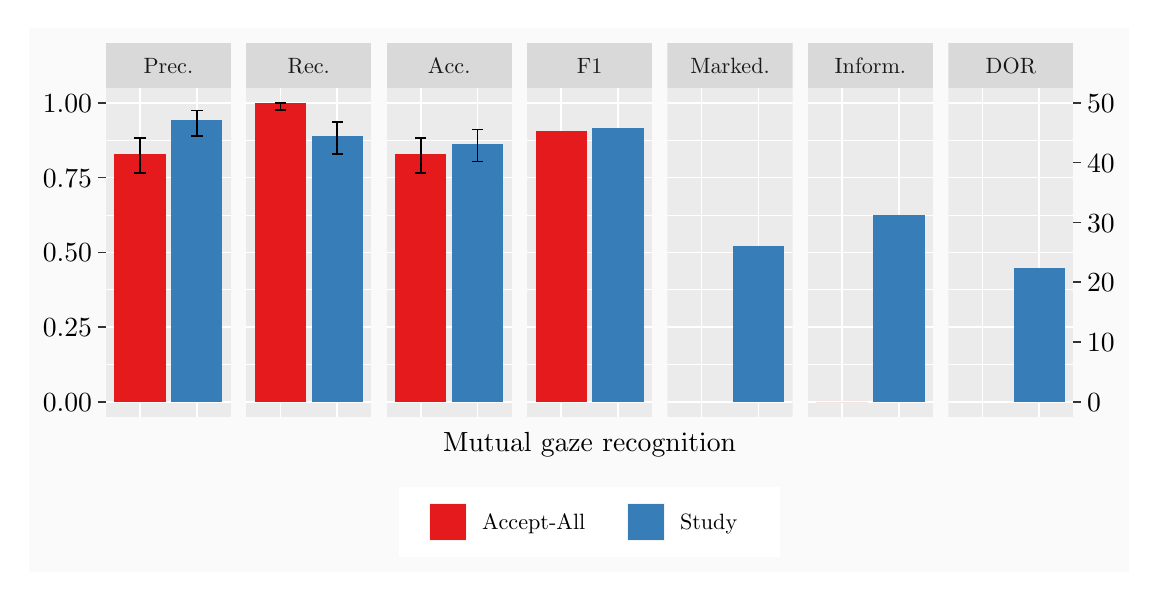
\begin{tikzpicture}[x=1pt,y=1pt]
\definecolor{fillColor}{RGB}{255,255,255}
\path[use as bounding box,fill=fillColor,fill opacity=0.00] (0,0) rectangle (398.34,196.94);
\begin{scope}
\path[clip] (  0.00,  0.00) rectangle (398.34,196.94);
\definecolor{drawColor}{RGB}{255,255,255}
\definecolor{fillColor}{gray}{0.98}

\path[draw=drawColor,line width= 0.6pt,line join=round,line cap=round,fill=fillColor] (  0.00,  0.00) rectangle (398.34,196.94);
\end{scope}
\begin{scope}
\path[clip] ( 28.22, 56.29) rectangle ( 73.46,175.18);
\definecolor{fillColor}{gray}{0.92}

\path[fill=fillColor] ( 28.22, 56.29) rectangle ( 73.46,175.18);
\definecolor{drawColor}{RGB}{255,255,255}

\path[draw=drawColor,line width= 0.3pt,line join=round] ( 28.22, 75.20) --
	( 73.46, 75.20);

\path[draw=drawColor,line width= 0.3pt,line join=round] ( 28.22,102.22) --
	( 73.46,102.22);

\path[draw=drawColor,line width= 0.3pt,line join=round] ( 28.22,129.25) --
	( 73.46,129.25);

\path[draw=drawColor,line width= 0.3pt,line join=round] ( 28.22,156.27) --
	( 73.46,156.27);

\path[draw=drawColor,line width= 0.6pt,line join=round] ( 28.22, 61.69) --
	( 73.46, 61.69);

\path[draw=drawColor,line width= 0.6pt,line join=round] ( 28.22, 88.71) --
	( 73.46, 88.71);

\path[draw=drawColor,line width= 0.6pt,line join=round] ( 28.22,115.74) --
	( 73.46,115.74);

\path[draw=drawColor,line width= 0.6pt,line join=round] ( 28.22,142.76) --
	( 73.46,142.76);

\path[draw=drawColor,line width= 0.6pt,line join=round] ( 28.22,169.78) --
	( 73.46,169.78);

\path[draw=drawColor,line width= 0.6pt,line join=round] ( 40.56, 56.29) --
	( 40.56,175.18);

\path[draw=drawColor,line width= 0.6pt,line join=round] ( 61.12, 56.29) --
	( 61.12,175.18);
\definecolor{fillColor}{RGB}{228,26,28}

\path[fill=fillColor] ( 31.31, 61.69) rectangle ( 49.81,151.36);
\definecolor{fillColor}{RGB}{55,126,184}

\path[fill=fillColor] ( 51.87, 61.69) rectangle ( 70.38,163.51);
\definecolor{drawColor}{RGB}{0,0,0}

\path[draw=drawColor,line width= 0.6pt,line join=round] ( 59.07,167.04) --
	( 63.18,167.04);

\path[draw=drawColor,line width= 0.6pt,line join=round] ( 61.12,167.04) --
	( 61.12,157.78);

\path[draw=drawColor,line width= 0.6pt,line join=round] ( 59.07,157.78) --
	( 63.18,157.78);

\path[draw=drawColor,line width= 0.6pt,line join=round] ( 38.50,157.02) --
	( 42.62,157.02);

\path[draw=drawColor,line width= 0.6pt,line join=round] ( 40.56,157.02) --
	( 40.56,144.45);

\path[draw=drawColor,line width= 0.6pt,line join=round] ( 38.50,144.45) --
	( 42.62,144.45);
\end{scope}
\begin{scope}
\path[clip] ( 78.96, 56.29) rectangle (124.20,175.18);
\definecolor{fillColor}{gray}{0.92}

\path[fill=fillColor] ( 78.96, 56.29) rectangle (124.20,175.18);
\definecolor{drawColor}{RGB}{255,255,255}

\path[draw=drawColor,line width= 0.3pt,line join=round] ( 78.96, 75.20) --
	(124.20, 75.20);

\path[draw=drawColor,line width= 0.3pt,line join=round] ( 78.96,102.22) --
	(124.20,102.22);

\path[draw=drawColor,line width= 0.3pt,line join=round] ( 78.96,129.25) --
	(124.20,129.25);

\path[draw=drawColor,line width= 0.3pt,line join=round] ( 78.96,156.27) --
	(124.20,156.27);

\path[draw=drawColor,line width= 0.6pt,line join=round] ( 78.96, 61.69) --
	(124.20, 61.69);

\path[draw=drawColor,line width= 0.6pt,line join=round] ( 78.96, 88.71) --
	(124.20, 88.71);

\path[draw=drawColor,line width= 0.6pt,line join=round] ( 78.96,115.74) --
	(124.20,115.74);

\path[draw=drawColor,line width= 0.6pt,line join=round] ( 78.96,142.76) --
	(124.20,142.76);

\path[draw=drawColor,line width= 0.6pt,line join=round] ( 78.96,169.78) --
	(124.20,169.78);

\path[draw=drawColor,line width= 0.6pt,line join=round] ( 91.30, 56.29) --
	( 91.30,175.18);

\path[draw=drawColor,line width= 0.6pt,line join=round] (111.86, 56.29) --
	(111.86,175.18);
\definecolor{fillColor}{RGB}{228,26,28}

\path[fill=fillColor] ( 82.05, 61.69) rectangle (100.55,169.78);
\definecolor{fillColor}{RGB}{55,126,184}

\path[fill=fillColor] (102.61, 61.69) rectangle (121.12,157.93);
\definecolor{drawColor}{RGB}{0,0,0}

\path[draw=drawColor,line width= 0.6pt,line join=round] (109.81,162.87) --
	(113.92,162.87);

\path[draw=drawColor,line width= 0.6pt,line join=round] (111.86,162.87) --
	(111.86,151.20);

\path[draw=drawColor,line width= 0.6pt,line join=round] (109.81,151.20) --
	(113.92,151.20);

\path[draw=drawColor,line width= 0.6pt,line join=round] ( 89.24,169.78) --
	( 93.36,169.78);

\path[draw=drawColor,line width= 0.6pt,line join=round] ( 91.30,169.78) --
	( 91.30,167.08);

\path[draw=drawColor,line width= 0.6pt,line join=round] ( 89.24,167.08) --
	( 93.36,167.08);
\end{scope}
\begin{scope}
\path[clip] (129.70, 56.29) rectangle (174.94,175.18);
\definecolor{fillColor}{gray}{0.92}

\path[fill=fillColor] (129.70, 56.29) rectangle (174.94,175.18);
\definecolor{drawColor}{RGB}{255,255,255}

\path[draw=drawColor,line width= 0.3pt,line join=round] (129.70, 75.20) --
	(174.94, 75.20);

\path[draw=drawColor,line width= 0.3pt,line join=round] (129.70,102.22) --
	(174.94,102.22);

\path[draw=drawColor,line width= 0.3pt,line join=round] (129.70,129.25) --
	(174.94,129.25);

\path[draw=drawColor,line width= 0.3pt,line join=round] (129.70,156.27) --
	(174.94,156.27);

\path[draw=drawColor,line width= 0.6pt,line join=round] (129.70, 61.69) --
	(174.94, 61.69);

\path[draw=drawColor,line width= 0.6pt,line join=round] (129.70, 88.71) --
	(174.94, 88.71);

\path[draw=drawColor,line width= 0.6pt,line join=round] (129.70,115.74) --
	(174.94,115.74);

\path[draw=drawColor,line width= 0.6pt,line join=round] (129.70,142.76) --
	(174.94,142.76);

\path[draw=drawColor,line width= 0.6pt,line join=round] (129.70,169.78) --
	(174.94,169.78);

\path[draw=drawColor,line width= 0.6pt,line join=round] (142.04, 56.29) --
	(142.04,175.18);

\path[draw=drawColor,line width= 0.6pt,line join=round] (162.60, 56.29) --
	(162.60,175.18);
\definecolor{fillColor}{RGB}{228,26,28}

\path[fill=fillColor] (132.78, 61.69) rectangle (151.29,151.36);
\definecolor{fillColor}{RGB}{55,126,184}

\path[fill=fillColor] (153.35, 61.69) rectangle (171.85,155.04);
\definecolor{drawColor}{RGB}{0,0,0}

\path[draw=drawColor,line width= 0.6pt,line join=round] (160.54,160.12) --
	(164.66,160.12);

\path[draw=drawColor,line width= 0.6pt,line join=round] (162.60,160.12) --
	(162.60,148.59);

\path[draw=drawColor,line width= 0.6pt,line join=round] (160.54,148.59) --
	(164.66,148.59);

\path[draw=drawColor,line width= 0.6pt,line join=round] (139.98,157.02) --
	(144.09,157.02);

\path[draw=drawColor,line width= 0.6pt,line join=round] (142.04,157.02) --
	(142.04,144.45);

\path[draw=drawColor,line width= 0.6pt,line join=round] (139.98,144.45) --
	(144.09,144.45);
\end{scope}
\begin{scope}
\path[clip] (180.44, 56.29) rectangle (225.68,175.18);
\definecolor{fillColor}{gray}{0.92}

\path[fill=fillColor] (180.44, 56.29) rectangle (225.68,175.18);
\definecolor{drawColor}{RGB}{255,255,255}

\path[draw=drawColor,line width= 0.3pt,line join=round] (180.44, 75.20) --
	(225.68, 75.20);

\path[draw=drawColor,line width= 0.3pt,line join=round] (180.44,102.22) --
	(225.68,102.22);

\path[draw=drawColor,line width= 0.3pt,line join=round] (180.44,129.25) --
	(225.68,129.25);

\path[draw=drawColor,line width= 0.3pt,line join=round] (180.44,156.27) --
	(225.68,156.27);

\path[draw=drawColor,line width= 0.6pt,line join=round] (180.44, 61.69) --
	(225.68, 61.69);

\path[draw=drawColor,line width= 0.6pt,line join=round] (180.44, 88.71) --
	(225.68, 88.71);

\path[draw=drawColor,line width= 0.6pt,line join=round] (180.44,115.74) --
	(225.68,115.74);

\path[draw=drawColor,line width= 0.6pt,line join=round] (180.44,142.76) --
	(225.68,142.76);

\path[draw=drawColor,line width= 0.6pt,line join=round] (180.44,169.78) --
	(225.68,169.78);

\path[draw=drawColor,line width= 0.6pt,line join=round] (192.78, 56.29) --
	(192.78,175.18);

\path[draw=drawColor,line width= 0.6pt,line join=round] (213.34, 56.29) --
	(213.34,175.18);
\definecolor{fillColor}{RGB}{228,26,28}

\path[fill=fillColor] (183.52, 61.69) rectangle (202.03,159.71);
\definecolor{fillColor}{RGB}{55,126,184}

\path[fill=fillColor] (204.09, 61.69) rectangle (222.59,160.65);
\end{scope}
\begin{scope}
\path[clip] (231.18, 56.29) rectangle (276.41,175.18);
\definecolor{fillColor}{gray}{0.92}

\path[fill=fillColor] (231.18, 56.29) rectangle (276.41,175.18);
\definecolor{drawColor}{RGB}{255,255,255}

\path[draw=drawColor,line width= 0.3pt,line join=round] (231.18, 75.20) --
	(276.41, 75.20);

\path[draw=drawColor,line width= 0.3pt,line join=round] (231.18,102.22) --
	(276.41,102.22);

\path[draw=drawColor,line width= 0.3pt,line join=round] (231.18,129.25) --
	(276.41,129.25);

\path[draw=drawColor,line width= 0.3pt,line join=round] (231.18,156.27) --
	(276.41,156.27);

\path[draw=drawColor,line width= 0.6pt,line join=round] (231.18, 61.69) --
	(276.41, 61.69);

\path[draw=drawColor,line width= 0.6pt,line join=round] (231.18, 88.71) --
	(276.41, 88.71);

\path[draw=drawColor,line width= 0.6pt,line join=round] (231.18,115.74) --
	(276.41,115.74);

\path[draw=drawColor,line width= 0.6pt,line join=round] (231.18,142.76) --
	(276.41,142.76);

\path[draw=drawColor,line width= 0.6pt,line join=round] (231.18,169.78) --
	(276.41,169.78);

\path[draw=drawColor,line width= 0.6pt,line join=round] (243.51, 56.29) --
	(243.51,175.18);

\path[draw=drawColor,line width= 0.6pt,line join=round] (264.08, 56.29) --
	(264.08,175.18);
\definecolor{fillColor}{RGB}{55,126,184}

\path[fill=fillColor] (254.82, 61.69) rectangle (273.33,118.00);
\end{scope}
\begin{scope}
\path[clip] (281.91, 56.29) rectangle (327.15,175.18);
\definecolor{fillColor}{gray}{0.92}

\path[fill=fillColor] (281.91, 56.29) rectangle (327.15,175.18);
\definecolor{drawColor}{RGB}{255,255,255}

\path[draw=drawColor,line width= 0.3pt,line join=round] (281.91, 75.20) --
	(327.15, 75.20);

\path[draw=drawColor,line width= 0.3pt,line join=round] (281.91,102.22) --
	(327.15,102.22);

\path[draw=drawColor,line width= 0.3pt,line join=round] (281.91,129.25) --
	(327.15,129.25);

\path[draw=drawColor,line width= 0.3pt,line join=round] (281.91,156.27) --
	(327.15,156.27);

\path[draw=drawColor,line width= 0.6pt,line join=round] (281.91, 61.69) --
	(327.15, 61.69);

\path[draw=drawColor,line width= 0.6pt,line join=round] (281.91, 88.71) --
	(327.15, 88.71);

\path[draw=drawColor,line width= 0.6pt,line join=round] (281.91,115.74) --
	(327.15,115.74);

\path[draw=drawColor,line width= 0.6pt,line join=round] (281.91,142.76) --
	(327.15,142.76);

\path[draw=drawColor,line width= 0.6pt,line join=round] (281.91,169.78) --
	(327.15,169.78);

\path[draw=drawColor,line width= 0.6pt,line join=round] (294.25, 56.29) --
	(294.25,175.18);

\path[draw=drawColor,line width= 0.6pt,line join=round] (314.82, 56.29) --
	(314.82,175.18);
\definecolor{fillColor}{RGB}{228,26,28}

\path[fill=fillColor] (285.00, 61.69) rectangle (303.51, 61.69);
\definecolor{fillColor}{RGB}{55,126,184}

\path[fill=fillColor] (305.56, 61.69) rectangle (324.07,129.11);
\end{scope}
\begin{scope}
\path[clip] (332.65, 56.29) rectangle (377.89,175.18);
\definecolor{fillColor}{gray}{0.92}

\path[fill=fillColor] (332.65, 56.29) rectangle (377.89,175.18);
\definecolor{drawColor}{RGB}{255,255,255}

\path[draw=drawColor,line width= 0.3pt,line join=round] (332.65, 75.20) --
	(377.89, 75.20);

\path[draw=drawColor,line width= 0.3pt,line join=round] (332.65,102.22) --
	(377.89,102.22);

\path[draw=drawColor,line width= 0.3pt,line join=round] (332.65,129.25) --
	(377.89,129.25);

\path[draw=drawColor,line width= 0.3pt,line join=round] (332.65,156.27) --
	(377.89,156.27);

\path[draw=drawColor,line width= 0.6pt,line join=round] (332.65, 61.69) --
	(377.89, 61.69);

\path[draw=drawColor,line width= 0.6pt,line join=round] (332.65, 88.71) --
	(377.89, 88.71);

\path[draw=drawColor,line width= 0.6pt,line join=round] (332.65,115.74) --
	(377.89,115.74);

\path[draw=drawColor,line width= 0.6pt,line join=round] (332.65,142.76) --
	(377.89,142.76);

\path[draw=drawColor,line width= 0.6pt,line join=round] (332.65,169.78) --
	(377.89,169.78);

\path[draw=drawColor,line width= 0.6pt,line join=round] (344.99, 56.29) --
	(344.99,175.18);

\path[draw=drawColor,line width= 0.6pt,line join=round] (365.55, 56.29) --
	(365.55,175.18);
\definecolor{fillColor}{RGB}{55,126,184}

\path[fill=fillColor] (356.30, 61.69) rectangle (374.81,109.99);
\end{scope}
\begin{scope}
\path[clip] ( 28.22,175.18) rectangle ( 73.46,191.44);
\definecolor{fillColor}{gray}{0.85}

\path[fill=fillColor] ( 28.22,175.18) rectangle ( 73.46,191.44);
\definecolor{drawColor}{gray}{0.10}

\node[text=drawColor,anchor=base,inner sep=0pt, outer sep=0pt, scale=  0.80] at ( 50.84,180.56) {Prec.};
\end{scope}
\begin{scope}
\path[clip] ( 78.96,175.18) rectangle (124.20,191.44);
\definecolor{fillColor}{gray}{0.85}

\path[fill=fillColor] ( 78.96,175.18) rectangle (124.20,191.44);
\definecolor{drawColor}{gray}{0.10}

\node[text=drawColor,anchor=base,inner sep=0pt, outer sep=0pt, scale=  0.80] at (101.58,180.56) {Rec.};
\end{scope}
\begin{scope}
\path[clip] (129.70,175.18) rectangle (174.94,191.44);
\definecolor{fillColor}{gray}{0.85}

\path[fill=fillColor] (129.70,175.18) rectangle (174.94,191.44);
\definecolor{drawColor}{gray}{0.10}

\node[text=drawColor,anchor=base,inner sep=0pt, outer sep=0pt, scale=  0.80] at (152.32,180.56) {Acc.};
\end{scope}
\begin{scope}
\path[clip] (180.44,175.18) rectangle (225.68,191.44);
\definecolor{fillColor}{gray}{0.85}

\path[fill=fillColor] (180.44,175.18) rectangle (225.68,191.44);
\definecolor{drawColor}{gray}{0.10}

\node[text=drawColor,anchor=base,inner sep=0pt, outer sep=0pt, scale=  0.80] at (203.06,180.56) {F1};
\end{scope}
\begin{scope}
\path[clip] (231.18,175.18) rectangle (276.41,191.44);
\definecolor{fillColor}{gray}{0.85}

\path[fill=fillColor] (231.18,175.18) rectangle (276.41,191.44);
\definecolor{drawColor}{gray}{0.10}

\node[text=drawColor,anchor=base,inner sep=0pt, outer sep=0pt, scale=  0.80] at (253.80,180.56) {Marked.};
\end{scope}
\begin{scope}
\path[clip] (281.91,175.18) rectangle (327.15,191.44);
\definecolor{fillColor}{gray}{0.85}

\path[fill=fillColor] (281.91,175.18) rectangle (327.15,191.44);
\definecolor{drawColor}{gray}{0.10}

\node[text=drawColor,anchor=base,inner sep=0pt, outer sep=0pt, scale=  0.80] at (304.53,180.56) {Inform.};
\end{scope}
\begin{scope}
\path[clip] (332.65,175.18) rectangle (377.89,191.44);
\definecolor{fillColor}{gray}{0.85}

\path[fill=fillColor] (332.65,175.18) rectangle (377.89,191.44);
\definecolor{drawColor}{gray}{0.10}

\node[text=drawColor,anchor=base,inner sep=0pt, outer sep=0pt, scale=  0.80] at (355.27,180.56) {DOR};
\end{scope}
\begin{scope}
\path[clip] (  0.00,  0.00) rectangle (398.34,196.94);
\definecolor{drawColor}{RGB}{0,0,0}

\node[text=drawColor,anchor=base east,inner sep=0pt, outer sep=0pt, scale=  1.00] at ( 23.27, 58.25) {0.00};

\node[text=drawColor,anchor=base east,inner sep=0pt, outer sep=0pt, scale=  1.00] at ( 23.27, 85.27) {0.25};

\node[text=drawColor,anchor=base east,inner sep=0pt, outer sep=0pt, scale=  1.00] at ( 23.27,112.29) {0.50};

\node[text=drawColor,anchor=base east,inner sep=0pt, outer sep=0pt, scale=  1.00] at ( 23.27,139.31) {0.75};

\node[text=drawColor,anchor=base east,inner sep=0pt, outer sep=0pt, scale=  1.00] at ( 23.27,166.34) {1.00};
\end{scope}
\begin{scope}
\path[clip] (  0.00,  0.00) rectangle (398.34,196.94);
\definecolor{drawColor}{gray}{0.20}

\path[draw=drawColor,line width= 0.6pt,line join=round] ( 25.47, 61.69) --
	( 28.22, 61.69);

\path[draw=drawColor,line width= 0.6pt,line join=round] ( 25.47, 88.71) --
	( 28.22, 88.71);

\path[draw=drawColor,line width= 0.6pt,line join=round] ( 25.47,115.74) --
	( 28.22,115.74);

\path[draw=drawColor,line width= 0.6pt,line join=round] ( 25.47,142.76) --
	( 28.22,142.76);

\path[draw=drawColor,line width= 0.6pt,line join=round] ( 25.47,169.78) --
	( 28.22,169.78);
\end{scope}
\begin{scope}
\path[clip] (  0.00,  0.00) rectangle (398.34,196.94);
\definecolor{drawColor}{gray}{0.20}

\path[draw=drawColor,line width= 0.6pt,line join=round] (377.89, 61.69) --
	(380.64, 61.69);

\path[draw=drawColor,line width= 0.6pt,line join=round] (377.89, 83.31) --
	(380.64, 83.31);

\path[draw=drawColor,line width= 0.6pt,line join=round] (377.89,104.93) --
	(380.64,104.93);

\path[draw=drawColor,line width= 0.6pt,line join=round] (377.89,126.54) --
	(380.64,126.54);

\path[draw=drawColor,line width= 0.6pt,line join=round] (377.89,148.16) --
	(380.64,148.16);

\path[draw=drawColor,line width= 0.6pt,line join=round] (377.89,169.78) --
	(380.64,169.78);
\end{scope}
\begin{scope}
\path[clip] (  0.00,  0.00) rectangle (398.34,196.94);
\definecolor{drawColor}{RGB}{0,0,0}

\node[text=drawColor,anchor=base west,inner sep=0pt, outer sep=0pt, scale=  1.00] at (382.84, 58.25) {0};

\node[text=drawColor,anchor=base west,inner sep=0pt, outer sep=0pt, scale=  1.00] at (382.84, 79.86) {10};

\node[text=drawColor,anchor=base west,inner sep=0pt, outer sep=0pt, scale=  1.00] at (382.84,101.48) {20};

\node[text=drawColor,anchor=base west,inner sep=0pt, outer sep=0pt, scale=  1.00] at (382.84,123.10) {30};

\node[text=drawColor,anchor=base west,inner sep=0pt, outer sep=0pt, scale=  1.00] at (382.84,144.72) {40};

\node[text=drawColor,anchor=base west,inner sep=0pt, outer sep=0pt, scale=  1.00] at (382.84,166.34) {50};
\end{scope}
\begin{scope}
\path[clip] (  0.00,  0.00) rectangle (398.34,196.94);
\definecolor{drawColor}{RGB}{0,0,0}

\node[text=drawColor,anchor=base,inner sep=0pt, outer sep=0pt, scale=  1.00] at (203.06, 43.90) {Mutual gaze recognition};
\end{scope}
\begin{scope}
\path[clip] (  0.00,  0.00) rectangle (398.34,196.94);
\definecolor{fillColor}{RGB}{255,255,255}

\path[fill=fillColor] (134.22,  5.50) rectangle (271.89, 30.95);
\end{scope}
\begin{scope}
\path[clip] (  0.00,  0.00) rectangle (398.34,196.94);
\definecolor{drawColor}{RGB}{255,255,255}
\definecolor{fillColor}{gray}{0.95}

\path[draw=drawColor,line width= 0.6pt,line join=round,line cap=round,fill=fillColor] (144.72, 11.00) rectangle (159.18, 25.45);
\end{scope}
\begin{scope}
\path[clip] (  0.00,  0.00) rectangle (398.34,196.94);
\definecolor{fillColor}{RGB}{228,26,28}

\path[fill=fillColor] (145.43, 11.71) rectangle (158.46, 24.74);
\end{scope}
\begin{scope}
\path[clip] (  0.00,  0.00) rectangle (398.34,196.94);
\definecolor{drawColor}{RGB}{255,255,255}
\definecolor{fillColor}{gray}{0.95}

\path[draw=drawColor,line width= 0.6pt,line join=round,line cap=round,fill=fillColor] (216.28, 11.00) rectangle (230.73, 25.45);
\end{scope}
\begin{scope}
\path[clip] (  0.00,  0.00) rectangle (398.34,196.94);
\definecolor{fillColor}{RGB}{55,126,184}

\path[fill=fillColor] (216.99, 11.71) rectangle (230.02, 24.74);
\end{scope}
\begin{scope}
\path[clip] (  0.00,  0.00) rectangle (398.34,196.94);
\definecolor{drawColor}{RGB}{0,0,0}

\node[text=drawColor,anchor=base west,inner sep=0pt, outer sep=0pt, scale=  0.80] at (164.18, 15.47) {Accept-All};
\end{scope}
\begin{scope}
\path[clip] (  0.00,  0.00) rectangle (398.34,196.94);
\definecolor{drawColor}{RGB}{0,0,0}

\node[text=drawColor,anchor=base west,inner sep=0pt, outer sep=0pt, scale=  0.80] at (235.73, 15.47) {Study};
\end{scope}
\end{tikzpicture}

      }
      \vspace{-70pt}
    \end{figure}
    \begin{figure}[htb]
      \resizebox{\textwidth}{!}{%
        % Created by tikzDevice version 0.12
% !TEX encoding = UTF-8 Unicode
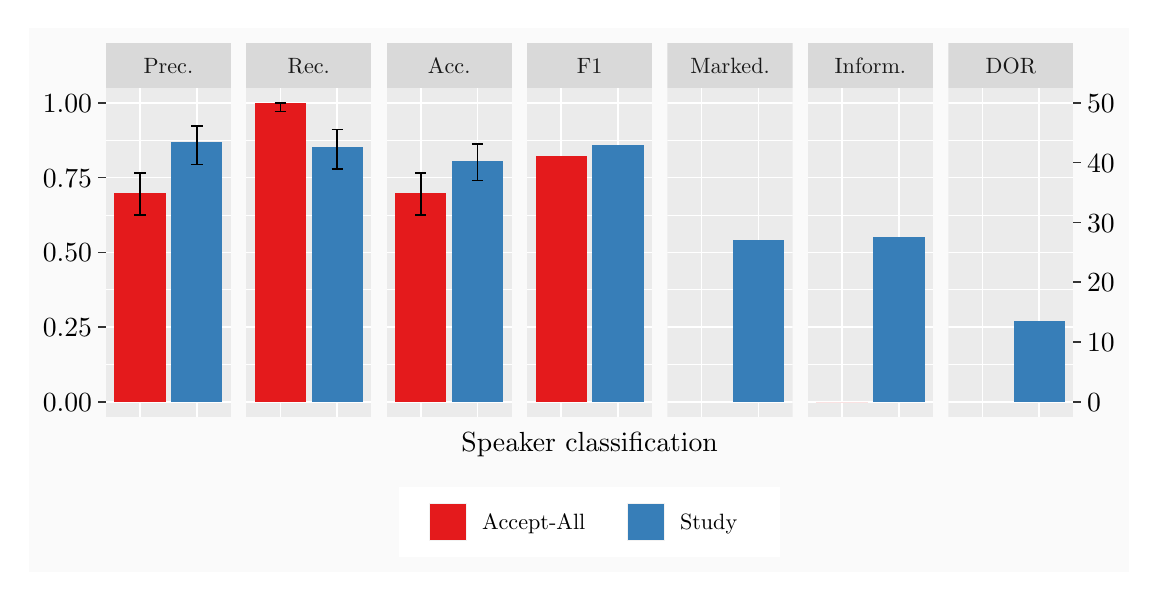
\begin{tikzpicture}[x=1pt,y=1pt]
\definecolor{fillColor}{RGB}{255,255,255}
\path[use as bounding box,fill=fillColor,fill opacity=0.00] (0,0) rectangle (398.34,196.94);
\begin{scope}
\path[clip] (  0.00,  0.00) rectangle (398.34,196.94);
\definecolor{drawColor}{RGB}{255,255,255}
\definecolor{fillColor}{gray}{0.98}

\path[draw=drawColor,line width= 0.6pt,line join=round,line cap=round,fill=fillColor] (  0.00,  0.00) rectangle (398.34,196.94);
\end{scope}
\begin{scope}
\path[clip] ( 28.22, 56.29) rectangle ( 73.46,175.18);
\definecolor{fillColor}{gray}{0.92}

\path[fill=fillColor] ( 28.22, 56.29) rectangle ( 73.46,175.18);
\definecolor{drawColor}{RGB}{255,255,255}

\path[draw=drawColor,line width= 0.3pt,line join=round] ( 28.22, 75.20) --
	( 73.46, 75.20);

\path[draw=drawColor,line width= 0.3pt,line join=round] ( 28.22,102.22) --
	( 73.46,102.22);

\path[draw=drawColor,line width= 0.3pt,line join=round] ( 28.22,129.25) --
	( 73.46,129.25);

\path[draw=drawColor,line width= 0.3pt,line join=round] ( 28.22,156.27) --
	( 73.46,156.27);

\path[draw=drawColor,line width= 0.6pt,line join=round] ( 28.22, 61.69) --
	( 73.46, 61.69);

\path[draw=drawColor,line width= 0.6pt,line join=round] ( 28.22, 88.71) --
	( 73.46, 88.71);

\path[draw=drawColor,line width= 0.6pt,line join=round] ( 28.22,115.74) --
	( 73.46,115.74);

\path[draw=drawColor,line width= 0.6pt,line join=round] ( 28.22,142.76) --
	( 73.46,142.76);

\path[draw=drawColor,line width= 0.6pt,line join=round] ( 28.22,169.78) --
	( 73.46,169.78);

\path[draw=drawColor,line width= 0.6pt,line join=round] ( 40.56, 56.29) --
	( 40.56,175.18);

\path[draw=drawColor,line width= 0.6pt,line join=round] ( 61.12, 56.29) --
	( 61.12,175.18);
\definecolor{fillColor}{RGB}{228,26,28}

\path[fill=fillColor] ( 31.31, 61.69) rectangle ( 49.81,137.23);
\definecolor{fillColor}{RGB}{55,126,184}

\path[fill=fillColor] ( 51.87, 61.69) rectangle ( 70.38,155.49);
\definecolor{drawColor}{RGB}{0,0,0}

\path[draw=drawColor,line width= 0.6pt,line join=round] ( 59.07,161.40) --
	( 63.18,161.40);

\path[draw=drawColor,line width= 0.6pt,line join=round] ( 61.12,161.40) --
	( 61.12,147.53);

\path[draw=drawColor,line width= 0.6pt,line join=round] ( 59.07,147.53) --
	( 63.18,147.53);

\path[draw=drawColor,line width= 0.6pt,line join=round] ( 38.50,144.44) --
	( 42.62,144.44);

\path[draw=drawColor,line width= 0.6pt,line join=round] ( 40.56,144.44) --
	( 40.56,129.28);

\path[draw=drawColor,line width= 0.6pt,line join=round] ( 38.50,129.28) --
	( 42.62,129.28);
\end{scope}
\begin{scope}
\path[clip] ( 78.96, 56.29) rectangle (124.20,175.18);
\definecolor{fillColor}{gray}{0.92}

\path[fill=fillColor] ( 78.96, 56.29) rectangle (124.20,175.18);
\definecolor{drawColor}{RGB}{255,255,255}

\path[draw=drawColor,line width= 0.3pt,line join=round] ( 78.96, 75.20) --
	(124.20, 75.20);

\path[draw=drawColor,line width= 0.3pt,line join=round] ( 78.96,102.22) --
	(124.20,102.22);

\path[draw=drawColor,line width= 0.3pt,line join=round] ( 78.96,129.25) --
	(124.20,129.25);

\path[draw=drawColor,line width= 0.3pt,line join=round] ( 78.96,156.27) --
	(124.20,156.27);

\path[draw=drawColor,line width= 0.6pt,line join=round] ( 78.96, 61.69) --
	(124.20, 61.69);

\path[draw=drawColor,line width= 0.6pt,line join=round] ( 78.96, 88.71) --
	(124.20, 88.71);

\path[draw=drawColor,line width= 0.6pt,line join=round] ( 78.96,115.74) --
	(124.20,115.74);

\path[draw=drawColor,line width= 0.6pt,line join=round] ( 78.96,142.76) --
	(124.20,142.76);

\path[draw=drawColor,line width= 0.6pt,line join=round] ( 78.96,169.78) --
	(124.20,169.78);

\path[draw=drawColor,line width= 0.6pt,line join=round] ( 91.30, 56.29) --
	( 91.30,175.18);

\path[draw=drawColor,line width= 0.6pt,line join=round] (111.86, 56.29) --
	(111.86,175.18);
\definecolor{fillColor}{RGB}{228,26,28}

\path[fill=fillColor] ( 82.05, 61.69) rectangle (100.55,169.78);
\definecolor{fillColor}{RGB}{55,126,184}

\path[fill=fillColor] (102.61, 61.69) rectangle (121.12,153.96);
\definecolor{drawColor}{RGB}{0,0,0}

\path[draw=drawColor,line width= 0.6pt,line join=round] (109.81,160.15) --
	(113.92,160.15);

\path[draw=drawColor,line width= 0.6pt,line join=round] (111.86,160.15) --
	(111.86,145.85);

\path[draw=drawColor,line width= 0.6pt,line join=round] (109.81,145.85) --
	(113.92,145.85);

\path[draw=drawColor,line width= 0.6pt,line join=round] ( 89.24,169.78) --
	( 93.36,169.78);

\path[draw=drawColor,line width= 0.6pt,line join=round] ( 91.30,169.78) --
	( 91.30,166.59);

\path[draw=drawColor,line width= 0.6pt,line join=round] ( 89.24,166.59) --
	( 93.36,166.59);
\end{scope}
\begin{scope}
\path[clip] (129.70, 56.29) rectangle (174.94,175.18);
\definecolor{fillColor}{gray}{0.92}

\path[fill=fillColor] (129.70, 56.29) rectangle (174.94,175.18);
\definecolor{drawColor}{RGB}{255,255,255}

\path[draw=drawColor,line width= 0.3pt,line join=round] (129.70, 75.20) --
	(174.94, 75.20);

\path[draw=drawColor,line width= 0.3pt,line join=round] (129.70,102.22) --
	(174.94,102.22);

\path[draw=drawColor,line width= 0.3pt,line join=round] (129.70,129.25) --
	(174.94,129.25);

\path[draw=drawColor,line width= 0.3pt,line join=round] (129.70,156.27) --
	(174.94,156.27);

\path[draw=drawColor,line width= 0.6pt,line join=round] (129.70, 61.69) --
	(174.94, 61.69);

\path[draw=drawColor,line width= 0.6pt,line join=round] (129.70, 88.71) --
	(174.94, 88.71);

\path[draw=drawColor,line width= 0.6pt,line join=round] (129.70,115.74) --
	(174.94,115.74);

\path[draw=drawColor,line width= 0.6pt,line join=round] (129.70,142.76) --
	(174.94,142.76);

\path[draw=drawColor,line width= 0.6pt,line join=round] (129.70,169.78) --
	(174.94,169.78);

\path[draw=drawColor,line width= 0.6pt,line join=round] (142.04, 56.29) --
	(142.04,175.18);

\path[draw=drawColor,line width= 0.6pt,line join=round] (162.60, 56.29) --
	(162.60,175.18);
\definecolor{fillColor}{RGB}{228,26,28}

\path[fill=fillColor] (132.78, 61.69) rectangle (151.29,137.23);
\definecolor{fillColor}{RGB}{55,126,184}

\path[fill=fillColor] (153.35, 61.69) rectangle (171.85,148.90);
\definecolor{drawColor}{RGB}{0,0,0}

\path[draw=drawColor,line width= 0.6pt,line join=round] (160.54,154.90) --
	(164.66,154.90);

\path[draw=drawColor,line width= 0.6pt,line join=round] (162.60,154.90) --
	(162.60,141.75);

\path[draw=drawColor,line width= 0.6pt,line join=round] (160.54,141.75) --
	(164.66,141.75);

\path[draw=drawColor,line width= 0.6pt,line join=round] (139.98,144.44) --
	(144.09,144.44);

\path[draw=drawColor,line width= 0.6pt,line join=round] (142.04,144.44) --
	(142.04,129.28);

\path[draw=drawColor,line width= 0.6pt,line join=round] (139.98,129.28) --
	(144.09,129.28);
\end{scope}
\begin{scope}
\path[clip] (180.44, 56.29) rectangle (225.68,175.18);
\definecolor{fillColor}{gray}{0.92}

\path[fill=fillColor] (180.44, 56.29) rectangle (225.68,175.18);
\definecolor{drawColor}{RGB}{255,255,255}

\path[draw=drawColor,line width= 0.3pt,line join=round] (180.44, 75.20) --
	(225.68, 75.20);

\path[draw=drawColor,line width= 0.3pt,line join=round] (180.44,102.22) --
	(225.68,102.22);

\path[draw=drawColor,line width= 0.3pt,line join=round] (180.44,129.25) --
	(225.68,129.25);

\path[draw=drawColor,line width= 0.3pt,line join=round] (180.44,156.27) --
	(225.68,156.27);

\path[draw=drawColor,line width= 0.6pt,line join=round] (180.44, 61.69) --
	(225.68, 61.69);

\path[draw=drawColor,line width= 0.6pt,line join=round] (180.44, 88.71) --
	(225.68, 88.71);

\path[draw=drawColor,line width= 0.6pt,line join=round] (180.44,115.74) --
	(225.68,115.74);

\path[draw=drawColor,line width= 0.6pt,line join=round] (180.44,142.76) --
	(225.68,142.76);

\path[draw=drawColor,line width= 0.6pt,line join=round] (180.44,169.78) --
	(225.68,169.78);

\path[draw=drawColor,line width= 0.6pt,line join=round] (192.78, 56.29) --
	(192.78,175.18);

\path[draw=drawColor,line width= 0.6pt,line join=round] (213.34, 56.29) --
	(213.34,175.18);
\definecolor{fillColor}{RGB}{228,26,28}

\path[fill=fillColor] (183.52, 61.69) rectangle (202.03,150.62);
\definecolor{fillColor}{RGB}{55,126,184}

\path[fill=fillColor] (204.09, 61.69) rectangle (222.59,154.72);
\end{scope}
\begin{scope}
\path[clip] (231.18, 56.29) rectangle (276.41,175.18);
\definecolor{fillColor}{gray}{0.92}

\path[fill=fillColor] (231.18, 56.29) rectangle (276.41,175.18);
\definecolor{drawColor}{RGB}{255,255,255}

\path[draw=drawColor,line width= 0.3pt,line join=round] (231.18, 75.20) --
	(276.41, 75.20);

\path[draw=drawColor,line width= 0.3pt,line join=round] (231.18,102.22) --
	(276.41,102.22);

\path[draw=drawColor,line width= 0.3pt,line join=round] (231.18,129.25) --
	(276.41,129.25);

\path[draw=drawColor,line width= 0.3pt,line join=round] (231.18,156.27) --
	(276.41,156.27);

\path[draw=drawColor,line width= 0.6pt,line join=round] (231.18, 61.69) --
	(276.41, 61.69);

\path[draw=drawColor,line width= 0.6pt,line join=round] (231.18, 88.71) --
	(276.41, 88.71);

\path[draw=drawColor,line width= 0.6pt,line join=round] (231.18,115.74) --
	(276.41,115.74);

\path[draw=drawColor,line width= 0.6pt,line join=round] (231.18,142.76) --
	(276.41,142.76);

\path[draw=drawColor,line width= 0.6pt,line join=round] (231.18,169.78) --
	(276.41,169.78);

\path[draw=drawColor,line width= 0.6pt,line join=round] (243.51, 56.29) --
	(243.51,175.18);

\path[draw=drawColor,line width= 0.6pt,line join=round] (264.08, 56.29) --
	(264.08,175.18);
\definecolor{fillColor}{RGB}{55,126,184}

\path[fill=fillColor] (254.82, 61.69) rectangle (273.33,120.11);
\end{scope}
\begin{scope}
\path[clip] (281.91, 56.29) rectangle (327.15,175.18);
\definecolor{fillColor}{gray}{0.92}

\path[fill=fillColor] (281.91, 56.29) rectangle (327.15,175.18);
\definecolor{drawColor}{RGB}{255,255,255}

\path[draw=drawColor,line width= 0.3pt,line join=round] (281.91, 75.20) --
	(327.15, 75.20);

\path[draw=drawColor,line width= 0.3pt,line join=round] (281.91,102.22) --
	(327.15,102.22);

\path[draw=drawColor,line width= 0.3pt,line join=round] (281.91,129.25) --
	(327.15,129.25);

\path[draw=drawColor,line width= 0.3pt,line join=round] (281.91,156.27) --
	(327.15,156.27);

\path[draw=drawColor,line width= 0.6pt,line join=round] (281.91, 61.69) --
	(327.15, 61.69);

\path[draw=drawColor,line width= 0.6pt,line join=round] (281.91, 88.71) --
	(327.15, 88.71);

\path[draw=drawColor,line width= 0.6pt,line join=round] (281.91,115.74) --
	(327.15,115.74);

\path[draw=drawColor,line width= 0.6pt,line join=round] (281.91,142.76) --
	(327.15,142.76);

\path[draw=drawColor,line width= 0.6pt,line join=round] (281.91,169.78) --
	(327.15,169.78);

\path[draw=drawColor,line width= 0.6pt,line join=round] (294.25, 56.29) --
	(294.25,175.18);

\path[draw=drawColor,line width= 0.6pt,line join=round] (314.82, 56.29) --
	(314.82,175.18);
\definecolor{fillColor}{RGB}{228,26,28}

\path[fill=fillColor] (285.00, 61.69) rectangle (303.51, 61.69);
\definecolor{fillColor}{RGB}{55,126,184}

\path[fill=fillColor] (305.56, 61.69) rectangle (324.07,121.33);
\end{scope}
\begin{scope}
\path[clip] (332.65, 56.29) rectangle (377.89,175.18);
\definecolor{fillColor}{gray}{0.92}

\path[fill=fillColor] (332.65, 56.29) rectangle (377.89,175.18);
\definecolor{drawColor}{RGB}{255,255,255}

\path[draw=drawColor,line width= 0.3pt,line join=round] (332.65, 75.20) --
	(377.89, 75.20);

\path[draw=drawColor,line width= 0.3pt,line join=round] (332.65,102.22) --
	(377.89,102.22);

\path[draw=drawColor,line width= 0.3pt,line join=round] (332.65,129.25) --
	(377.89,129.25);

\path[draw=drawColor,line width= 0.3pt,line join=round] (332.65,156.27) --
	(377.89,156.27);

\path[draw=drawColor,line width= 0.6pt,line join=round] (332.65, 61.69) --
	(377.89, 61.69);

\path[draw=drawColor,line width= 0.6pt,line join=round] (332.65, 88.71) --
	(377.89, 88.71);

\path[draw=drawColor,line width= 0.6pt,line join=round] (332.65,115.74) --
	(377.89,115.74);

\path[draw=drawColor,line width= 0.6pt,line join=round] (332.65,142.76) --
	(377.89,142.76);

\path[draw=drawColor,line width= 0.6pt,line join=round] (332.65,169.78) --
	(377.89,169.78);

\path[draw=drawColor,line width= 0.6pt,line join=round] (344.99, 56.29) --
	(344.99,175.18);

\path[draw=drawColor,line width= 0.6pt,line join=round] (365.55, 56.29) --
	(365.55,175.18);
\definecolor{fillColor}{RGB}{55,126,184}

\path[fill=fillColor] (356.30, 61.69) rectangle (374.81, 90.85);
\end{scope}
\begin{scope}
\path[clip] ( 28.22,175.18) rectangle ( 73.46,191.44);
\definecolor{fillColor}{gray}{0.85}

\path[fill=fillColor] ( 28.22,175.18) rectangle ( 73.46,191.44);
\definecolor{drawColor}{gray}{0.10}

\node[text=drawColor,anchor=base,inner sep=0pt, outer sep=0pt, scale=  0.80] at ( 50.84,180.56) {Prec.};
\end{scope}
\begin{scope}
\path[clip] ( 78.96,175.18) rectangle (124.20,191.44);
\definecolor{fillColor}{gray}{0.85}

\path[fill=fillColor] ( 78.96,175.18) rectangle (124.20,191.44);
\definecolor{drawColor}{gray}{0.10}

\node[text=drawColor,anchor=base,inner sep=0pt, outer sep=0pt, scale=  0.80] at (101.58,180.56) {Rec.};
\end{scope}
\begin{scope}
\path[clip] (129.70,175.18) rectangle (174.94,191.44);
\definecolor{fillColor}{gray}{0.85}

\path[fill=fillColor] (129.70,175.18) rectangle (174.94,191.44);
\definecolor{drawColor}{gray}{0.10}

\node[text=drawColor,anchor=base,inner sep=0pt, outer sep=0pt, scale=  0.80] at (152.32,180.56) {Acc.};
\end{scope}
\begin{scope}
\path[clip] (180.44,175.18) rectangle (225.68,191.44);
\definecolor{fillColor}{gray}{0.85}

\path[fill=fillColor] (180.44,175.18) rectangle (225.68,191.44);
\definecolor{drawColor}{gray}{0.10}

\node[text=drawColor,anchor=base,inner sep=0pt, outer sep=0pt, scale=  0.80] at (203.06,180.56) {F1};
\end{scope}
\begin{scope}
\path[clip] (231.18,175.18) rectangle (276.41,191.44);
\definecolor{fillColor}{gray}{0.85}

\path[fill=fillColor] (231.18,175.18) rectangle (276.41,191.44);
\definecolor{drawColor}{gray}{0.10}

\node[text=drawColor,anchor=base,inner sep=0pt, outer sep=0pt, scale=  0.80] at (253.80,180.56) {Marked.};
\end{scope}
\begin{scope}
\path[clip] (281.91,175.18) rectangle (327.15,191.44);
\definecolor{fillColor}{gray}{0.85}

\path[fill=fillColor] (281.91,175.18) rectangle (327.15,191.44);
\definecolor{drawColor}{gray}{0.10}

\node[text=drawColor,anchor=base,inner sep=0pt, outer sep=0pt, scale=  0.80] at (304.53,180.56) {Inform.};
\end{scope}
\begin{scope}
\path[clip] (332.65,175.18) rectangle (377.89,191.44);
\definecolor{fillColor}{gray}{0.85}

\path[fill=fillColor] (332.65,175.18) rectangle (377.89,191.44);
\definecolor{drawColor}{gray}{0.10}

\node[text=drawColor,anchor=base,inner sep=0pt, outer sep=0pt, scale=  0.80] at (355.27,180.56) {DOR};
\end{scope}
\begin{scope}
\path[clip] (  0.00,  0.00) rectangle (398.34,196.94);
\definecolor{drawColor}{RGB}{0,0,0}

\node[text=drawColor,anchor=base east,inner sep=0pt, outer sep=0pt, scale=  1.00] at ( 23.27, 58.25) {0.00};

\node[text=drawColor,anchor=base east,inner sep=0pt, outer sep=0pt, scale=  1.00] at ( 23.27, 85.27) {0.25};

\node[text=drawColor,anchor=base east,inner sep=0pt, outer sep=0pt, scale=  1.00] at ( 23.27,112.29) {0.50};

\node[text=drawColor,anchor=base east,inner sep=0pt, outer sep=0pt, scale=  1.00] at ( 23.27,139.31) {0.75};

\node[text=drawColor,anchor=base east,inner sep=0pt, outer sep=0pt, scale=  1.00] at ( 23.27,166.34) {1.00};
\end{scope}
\begin{scope}
\path[clip] (  0.00,  0.00) rectangle (398.34,196.94);
\definecolor{drawColor}{gray}{0.20}

\path[draw=drawColor,line width= 0.6pt,line join=round] ( 25.47, 61.69) --
	( 28.22, 61.69);

\path[draw=drawColor,line width= 0.6pt,line join=round] ( 25.47, 88.71) --
	( 28.22, 88.71);

\path[draw=drawColor,line width= 0.6pt,line join=round] ( 25.47,115.74) --
	( 28.22,115.74);

\path[draw=drawColor,line width= 0.6pt,line join=round] ( 25.47,142.76) --
	( 28.22,142.76);

\path[draw=drawColor,line width= 0.6pt,line join=round] ( 25.47,169.78) --
	( 28.22,169.78);
\end{scope}
\begin{scope}
\path[clip] (  0.00,  0.00) rectangle (398.34,196.94);
\definecolor{drawColor}{gray}{0.20}

\path[draw=drawColor,line width= 0.6pt,line join=round] (377.89, 61.69) --
	(380.64, 61.69);

\path[draw=drawColor,line width= 0.6pt,line join=round] (377.89, 83.31) --
	(380.64, 83.31);

\path[draw=drawColor,line width= 0.6pt,line join=round] (377.89,104.93) --
	(380.64,104.93);

\path[draw=drawColor,line width= 0.6pt,line join=round] (377.89,126.54) --
	(380.64,126.54);

\path[draw=drawColor,line width= 0.6pt,line join=round] (377.89,148.16) --
	(380.64,148.16);

\path[draw=drawColor,line width= 0.6pt,line join=round] (377.89,169.78) --
	(380.64,169.78);
\end{scope}
\begin{scope}
\path[clip] (  0.00,  0.00) rectangle (398.34,196.94);
\definecolor{drawColor}{RGB}{0,0,0}

\node[text=drawColor,anchor=base west,inner sep=0pt, outer sep=0pt, scale=  1.00] at (382.84, 58.25) {0};

\node[text=drawColor,anchor=base west,inner sep=0pt, outer sep=0pt, scale=  1.00] at (382.84, 79.86) {10};

\node[text=drawColor,anchor=base west,inner sep=0pt, outer sep=0pt, scale=  1.00] at (382.84,101.48) {20};

\node[text=drawColor,anchor=base west,inner sep=0pt, outer sep=0pt, scale=  1.00] at (382.84,123.10) {30};

\node[text=drawColor,anchor=base west,inner sep=0pt, outer sep=0pt, scale=  1.00] at (382.84,144.72) {40};

\node[text=drawColor,anchor=base west,inner sep=0pt, outer sep=0pt, scale=  1.00] at (382.84,166.34) {50};
\end{scope}
\begin{scope}
\path[clip] (  0.00,  0.00) rectangle (398.34,196.94);
\definecolor{drawColor}{RGB}{0,0,0}

\node[text=drawColor,anchor=base,inner sep=0pt, outer sep=0pt, scale=  1.00] at (203.06, 43.90) {Speaker classification};
\end{scope}
\begin{scope}
\path[clip] (  0.00,  0.00) rectangle (398.34,196.94);
\definecolor{fillColor}{RGB}{255,255,255}

\path[fill=fillColor] (134.22,  5.50) rectangle (271.89, 30.95);
\end{scope}
\begin{scope}
\path[clip] (  0.00,  0.00) rectangle (398.34,196.94);
\definecolor{drawColor}{RGB}{255,255,255}
\definecolor{fillColor}{gray}{0.95}

\path[draw=drawColor,line width= 0.6pt,line join=round,line cap=round,fill=fillColor] (144.72, 11.00) rectangle (159.18, 25.45);
\end{scope}
\begin{scope}
\path[clip] (  0.00,  0.00) rectangle (398.34,196.94);
\definecolor{fillColor}{RGB}{228,26,28}

\path[fill=fillColor] (145.43, 11.71) rectangle (158.46, 24.74);
\end{scope}
\begin{scope}
\path[clip] (  0.00,  0.00) rectangle (398.34,196.94);
\definecolor{drawColor}{RGB}{255,255,255}
\definecolor{fillColor}{gray}{0.95}

\path[draw=drawColor,line width= 0.6pt,line join=round,line cap=round,fill=fillColor] (216.28, 11.00) rectangle (230.73, 25.45);
\end{scope}
\begin{scope}
\path[clip] (  0.00,  0.00) rectangle (398.34,196.94);
\definecolor{fillColor}{RGB}{55,126,184}

\path[fill=fillColor] (216.99, 11.71) rectangle (230.02, 24.74);
\end{scope}
\begin{scope}
\path[clip] (  0.00,  0.00) rectangle (398.34,196.94);
\definecolor{drawColor}{RGB}{0,0,0}

\node[text=drawColor,anchor=base west,inner sep=0pt, outer sep=0pt, scale=  0.80] at (164.18, 15.47) {Accept-All};
\end{scope}
\begin{scope}
\path[clip] (  0.00,  0.00) rectangle (398.34,196.94);
\definecolor{drawColor}{RGB}{0,0,0}

\node[text=drawColor,anchor=base west,inner sep=0pt, outer sep=0pt, scale=  0.80] at (235.73, 15.47) {Study};
\end{scope}
\end{tikzpicture}

      }
    \end{figure}
    \end{column}%
      \begin{column}{.5\textwidth}
        \begin{center}
        \begin{scriptsize}
          Mutual Gaze Recognition
          \\ \vspace{10pt}
          \begin{tabular}{l | c | c }
                  & Baseline & Study \\ \hline
            \(P\) &  0.766 - 0.882&   \textbf{0.889 - 0.975} \\ 
            \(R\) &  \textbf{0.975 - 1.000} &  0.828 - 0.936 \\
           \end{tabular}
          \\ \vspace{10pt}
          \(M(G_S) = 0.52 \)\quad\(I(G_S) = 0.62\)\quad\( DOR(G_S) = 22\)
          \\ \vspace{10pt}
          Speaker classification
          \\ \vspace{10pt}
          \begin{tabular}{l | c | c }
                  & Baseline & Study \\ \hline
            \(P\) &  0.625 - 0.766 &   \textbf{0.794 - 0.922} \\ 
            \(R\) &  \textbf{0.970 - 1.00} &  0.779 - 0.911 \\
           \end{tabular}
          \\ \vspace{10pt}
          \(M(S_S) = 0.54 \)\quad\(I(S_S) = 0.55\)\quad\( DOR(S_S) = 13\)
          \end{scriptsize}
        \end{center}
   \end{column}%
   \end{columns}
  \end{frame}
  \begin{frame}{Addressee from mutual gaze \tiny{with 5\% confidence intervals}}
    \begin{columns}[T] % align columns
      \begin{column}{.5\textwidth}
        \begin{figure}[htb]
          \resizebox{\textwidth}{!}{%
            % Created by tikzDevice version 0.12
% !TEX encoding = UTF-8 Unicode
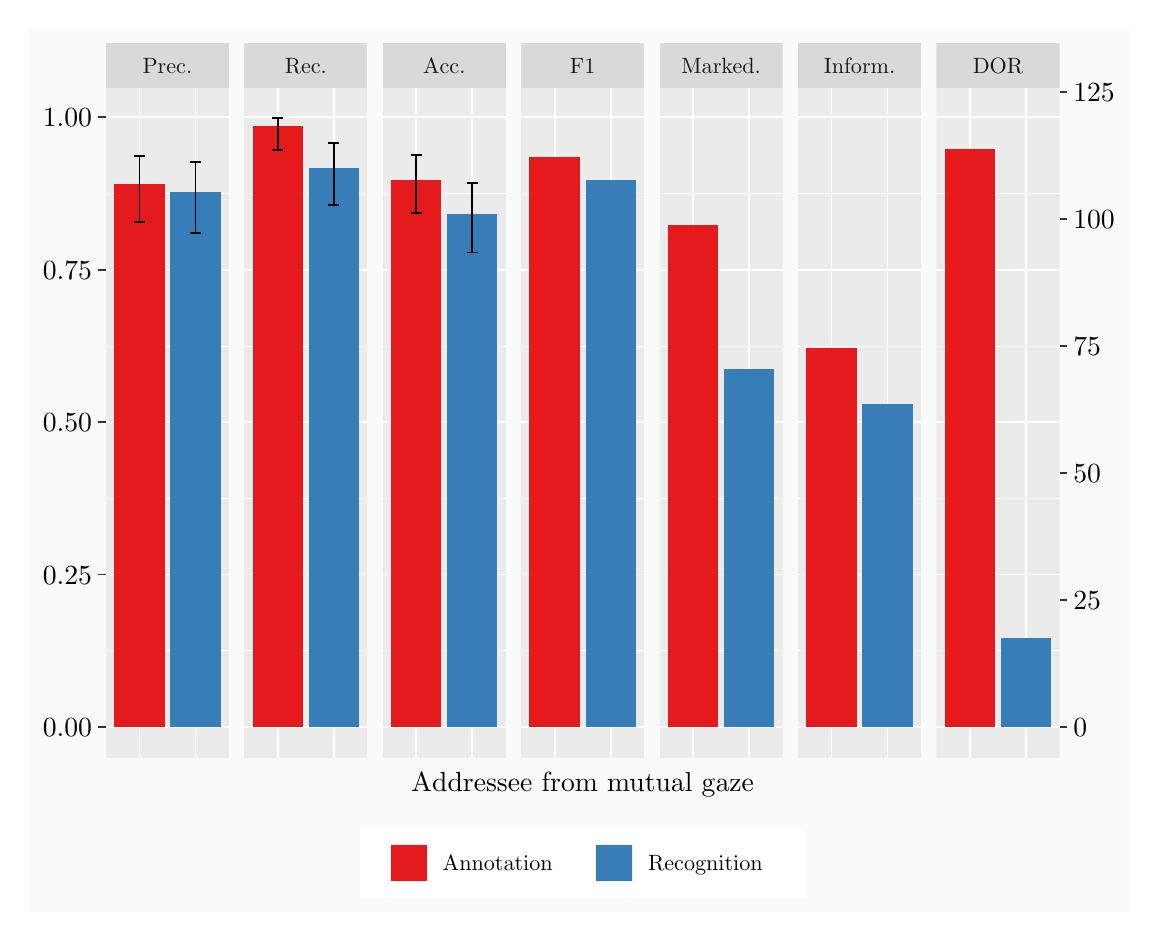
\begin{tikzpicture}[x=1pt,y=1pt]
\definecolor{fillColor}{RGB}{255,255,255}
\path[use as bounding box,fill=fillColor,fill opacity=0.00] (0,0) rectangle (398.34,320.03);
\begin{scope}
\path[clip] (  0.00,  0.00) rectangle (398.34,320.03);
\definecolor{drawColor}{RGB}{255,255,255}
\definecolor{fillColor}{gray}{0.98}

\path[draw=drawColor,line width= 0.6pt,line join=round,line cap=round,fill=fillColor] (  0.00,  0.00) rectangle (398.34,320.03);
\end{scope}
\begin{scope}
\path[clip] ( 28.22, 56.29) rectangle ( 72.75,298.27);
\definecolor{fillColor}{gray}{0.92}

\path[fill=fillColor] ( 28.22, 56.29) rectangle ( 72.75,298.27);
\definecolor{drawColor}{RGB}{255,255,255}

\path[draw=drawColor,line width= 0.3pt,line join=round] ( 28.22, 94.83) --
	( 72.75, 94.83);

\path[draw=drawColor,line width= 0.3pt,line join=round] ( 28.22,149.93) --
	( 72.75,149.93);

\path[draw=drawColor,line width= 0.3pt,line join=round] ( 28.22,205.03) --
	( 72.75,205.03);

\path[draw=drawColor,line width= 0.3pt,line join=round] ( 28.22,260.13) --
	( 72.75,260.13);

\path[draw=drawColor,line width= 0.6pt,line join=round] ( 28.22, 67.28) --
	( 72.75, 67.28);

\path[draw=drawColor,line width= 0.6pt,line join=round] ( 28.22,122.38) --
	( 72.75,122.38);

\path[draw=drawColor,line width= 0.6pt,line join=round] ( 28.22,177.48) --
	( 72.75,177.48);

\path[draw=drawColor,line width= 0.6pt,line join=round] ( 28.22,232.58) --
	( 72.75,232.58);

\path[draw=drawColor,line width= 0.6pt,line join=round] ( 28.22,287.68) --
	( 72.75,287.68);

\path[draw=drawColor,line width= 0.6pt,line join=round] ( 40.37, 56.29) --
	( 40.37,298.27);

\path[draw=drawColor,line width= 0.6pt,line join=round] ( 60.60, 56.29) --
	( 60.60,298.27);
\definecolor{fillColor}{RGB}{228,26,28}

\path[fill=fillColor] ( 31.26, 67.28) rectangle ( 49.47,263.53);
\definecolor{fillColor}{RGB}{55,126,184}

\path[fill=fillColor] ( 51.50, 67.28) rectangle ( 69.71,260.53);
\definecolor{drawColor}{RGB}{0,0,0}

\path[draw=drawColor,line width= 0.6pt,line join=round] ( 58.58,271.49) --
	( 62.63,271.49);

\path[draw=drawColor,line width= 0.6pt,line join=round] ( 60.60,271.49) --
	( 60.60,245.83);

\path[draw=drawColor,line width= 0.6pt,line join=round] ( 58.58,245.83) --
	( 62.63,245.83);

\path[draw=drawColor,line width= 0.6pt,line join=round] ( 38.34,273.58) --
	( 42.39,273.58);

\path[draw=drawColor,line width= 0.6pt,line join=round] ( 40.37,273.58) --
	( 40.37,249.80);

\path[draw=drawColor,line width= 0.6pt,line join=round] ( 38.34,249.80) --
	( 42.39,249.80);
\end{scope}
\begin{scope}
\path[clip] ( 78.25, 56.29) rectangle (122.77,298.27);
\definecolor{fillColor}{gray}{0.92}

\path[fill=fillColor] ( 78.25, 56.29) rectangle (122.77,298.27);
\definecolor{drawColor}{RGB}{255,255,255}

\path[draw=drawColor,line width= 0.3pt,line join=round] ( 78.25, 94.83) --
	(122.77, 94.83);

\path[draw=drawColor,line width= 0.3pt,line join=round] ( 78.25,149.93) --
	(122.77,149.93);

\path[draw=drawColor,line width= 0.3pt,line join=round] ( 78.25,205.03) --
	(122.77,205.03);

\path[draw=drawColor,line width= 0.3pt,line join=round] ( 78.25,260.13) --
	(122.77,260.13);

\path[draw=drawColor,line width= 0.6pt,line join=round] ( 78.25, 67.28) --
	(122.77, 67.28);

\path[draw=drawColor,line width= 0.6pt,line join=round] ( 78.25,122.38) --
	(122.77,122.38);

\path[draw=drawColor,line width= 0.6pt,line join=round] ( 78.25,177.48) --
	(122.77,177.48);

\path[draw=drawColor,line width= 0.6pt,line join=round] ( 78.25,232.58) --
	(122.77,232.58);

\path[draw=drawColor,line width= 0.6pt,line join=round] ( 78.25,287.68) --
	(122.77,287.68);

\path[draw=drawColor,line width= 0.6pt,line join=round] ( 90.39, 56.29) --
	( 90.39,298.27);

\path[draw=drawColor,line width= 0.6pt,line join=round] (110.63, 56.29) --
	(110.63,298.27);
\definecolor{fillColor}{RGB}{228,26,28}

\path[fill=fillColor] ( 81.28, 67.28) rectangle ( 99.50,284.34);
\definecolor{fillColor}{RGB}{55,126,184}

\path[fill=fillColor] (101.52, 67.28) rectangle (119.74,269.31);
\definecolor{drawColor}{RGB}{0,0,0}

\path[draw=drawColor,line width= 0.6pt,line join=round] (108.60,278.35) --
	(112.65,278.35);

\path[draw=drawColor,line width= 0.6pt,line join=round] (110.63,278.35) --
	(110.63,255.89);

\path[draw=drawColor,line width= 0.6pt,line join=round] (108.60,255.89) --
	(112.65,255.89);

\path[draw=drawColor,line width= 0.6pt,line join=round] ( 88.37,287.27) --
	( 92.41,287.27);

\path[draw=drawColor,line width= 0.6pt,line join=round] ( 90.39,287.27) --
	( 90.39,275.85);

\path[draw=drawColor,line width= 0.6pt,line join=round] ( 88.37,275.85) --
	( 92.41,275.85);
\end{scope}
\begin{scope}
\path[clip] (128.27, 56.29) rectangle (172.80,298.27);
\definecolor{fillColor}{gray}{0.92}

\path[fill=fillColor] (128.27, 56.29) rectangle (172.80,298.27);
\definecolor{drawColor}{RGB}{255,255,255}

\path[draw=drawColor,line width= 0.3pt,line join=round] (128.27, 94.83) --
	(172.80, 94.83);

\path[draw=drawColor,line width= 0.3pt,line join=round] (128.27,149.93) --
	(172.80,149.93);

\path[draw=drawColor,line width= 0.3pt,line join=round] (128.27,205.03) --
	(172.80,205.03);

\path[draw=drawColor,line width= 0.3pt,line join=round] (128.27,260.13) --
	(172.80,260.13);

\path[draw=drawColor,line width= 0.6pt,line join=round] (128.27, 67.28) --
	(172.80, 67.28);

\path[draw=drawColor,line width= 0.6pt,line join=round] (128.27,122.38) --
	(172.80,122.38);

\path[draw=drawColor,line width= 0.6pt,line join=round] (128.27,177.48) --
	(172.80,177.48);

\path[draw=drawColor,line width= 0.6pt,line join=round] (128.27,232.58) --
	(172.80,232.58);

\path[draw=drawColor,line width= 0.6pt,line join=round] (128.27,287.68) --
	(172.80,287.68);

\path[draw=drawColor,line width= 0.6pt,line join=round] (140.41, 56.29) --
	(140.41,298.27);

\path[draw=drawColor,line width= 0.6pt,line join=round] (160.65, 56.29) --
	(160.65,298.27);
\definecolor{fillColor}{RGB}{228,26,28}

\path[fill=fillColor] (131.31, 67.28) rectangle (149.52,265.14);
\definecolor{fillColor}{RGB}{55,126,184}

\path[fill=fillColor] (151.55, 67.28) rectangle (169.76,252.62);
\definecolor{drawColor}{RGB}{0,0,0}

\path[draw=drawColor,line width= 0.6pt,line join=round] (158.63,263.79) --
	(162.68,263.79);

\path[draw=drawColor,line width= 0.6pt,line join=round] (160.65,263.79) --
	(160.65,238.83);

\path[draw=drawColor,line width= 0.6pt,line join=round] (158.63,238.83) --
	(162.68,238.83);

\path[draw=drawColor,line width= 0.6pt,line join=round] (138.39,274.07) --
	(142.44,274.07);

\path[draw=drawColor,line width= 0.6pt,line join=round] (140.41,274.07) --
	(140.41,253.12);

\path[draw=drawColor,line width= 0.6pt,line join=round] (138.39,253.12) --
	(142.44,253.12);
\end{scope}
\begin{scope}
\path[clip] (178.30, 56.29) rectangle (222.82,298.27);
\definecolor{fillColor}{gray}{0.92}

\path[fill=fillColor] (178.30, 56.29) rectangle (222.82,298.27);
\definecolor{drawColor}{RGB}{255,255,255}

\path[draw=drawColor,line width= 0.3pt,line join=round] (178.30, 94.83) --
	(222.82, 94.83);

\path[draw=drawColor,line width= 0.3pt,line join=round] (178.30,149.93) --
	(222.82,149.93);

\path[draw=drawColor,line width= 0.3pt,line join=round] (178.30,205.03) --
	(222.82,205.03);

\path[draw=drawColor,line width= 0.3pt,line join=round] (178.30,260.13) --
	(222.82,260.13);

\path[draw=drawColor,line width= 0.6pt,line join=round] (178.30, 67.28) --
	(222.82, 67.28);

\path[draw=drawColor,line width= 0.6pt,line join=round] (178.30,122.38) --
	(222.82,122.38);

\path[draw=drawColor,line width= 0.6pt,line join=round] (178.30,177.48) --
	(222.82,177.48);

\path[draw=drawColor,line width= 0.6pt,line join=round] (178.30,232.58) --
	(222.82,232.58);

\path[draw=drawColor,line width= 0.6pt,line join=round] (178.30,287.68) --
	(222.82,287.68);

\path[draw=drawColor,line width= 0.6pt,line join=round] (190.44, 56.29) --
	(190.44,298.27);

\path[draw=drawColor,line width= 0.6pt,line join=round] (210.68, 56.29) --
	(210.68,298.27);
\definecolor{fillColor}{RGB}{228,26,28}

\path[fill=fillColor] (181.33, 67.28) rectangle (199.55,273.41);
\definecolor{fillColor}{RGB}{55,126,184}

\path[fill=fillColor] (201.57, 67.28) rectangle (219.78,264.82);
\end{scope}
\begin{scope}
\path[clip] (228.32, 56.29) rectangle (272.84,298.27);
\definecolor{fillColor}{gray}{0.92}

\path[fill=fillColor] (228.32, 56.29) rectangle (272.84,298.27);
\definecolor{drawColor}{RGB}{255,255,255}

\path[draw=drawColor,line width= 0.3pt,line join=round] (228.32, 94.83) --
	(272.84, 94.83);

\path[draw=drawColor,line width= 0.3pt,line join=round] (228.32,149.93) --
	(272.84,149.93);

\path[draw=drawColor,line width= 0.3pt,line join=round] (228.32,205.03) --
	(272.84,205.03);

\path[draw=drawColor,line width= 0.3pt,line join=round] (228.32,260.13) --
	(272.84,260.13);

\path[draw=drawColor,line width= 0.6pt,line join=round] (228.32, 67.28) --
	(272.84, 67.28);

\path[draw=drawColor,line width= 0.6pt,line join=round] (228.32,122.38) --
	(272.84,122.38);

\path[draw=drawColor,line width= 0.6pt,line join=round] (228.32,177.48) --
	(272.84,177.48);

\path[draw=drawColor,line width= 0.6pt,line join=round] (228.32,232.58) --
	(272.84,232.58);

\path[draw=drawColor,line width= 0.6pt,line join=round] (228.32,287.68) --
	(272.84,287.68);

\path[draw=drawColor,line width= 0.6pt,line join=round] (240.46, 56.29) --
	(240.46,298.27);

\path[draw=drawColor,line width= 0.6pt,line join=round] (260.70, 56.29) --
	(260.70,298.27);
\definecolor{fillColor}{RGB}{228,26,28}

\path[fill=fillColor] (231.36, 67.28) rectangle (249.57,248.83);
\definecolor{fillColor}{RGB}{55,126,184}

\path[fill=fillColor] (251.59, 67.28) rectangle (269.81,196.73);
\end{scope}
\begin{scope}
\path[clip] (278.34, 56.29) rectangle (322.87,298.27);
\definecolor{fillColor}{gray}{0.92}

\path[fill=fillColor] (278.34, 56.29) rectangle (322.87,298.27);
\definecolor{drawColor}{RGB}{255,255,255}

\path[draw=drawColor,line width= 0.3pt,line join=round] (278.34, 94.83) --
	(322.87, 94.83);

\path[draw=drawColor,line width= 0.3pt,line join=round] (278.34,149.93) --
	(322.87,149.93);

\path[draw=drawColor,line width= 0.3pt,line join=round] (278.34,205.03) --
	(322.87,205.03);

\path[draw=drawColor,line width= 0.3pt,line join=round] (278.34,260.13) --
	(322.87,260.13);

\path[draw=drawColor,line width= 0.6pt,line join=round] (278.34, 67.28) --
	(322.87, 67.28);

\path[draw=drawColor,line width= 0.6pt,line join=round] (278.34,122.38) --
	(322.87,122.38);

\path[draw=drawColor,line width= 0.6pt,line join=round] (278.34,177.48) --
	(322.87,177.48);

\path[draw=drawColor,line width= 0.6pt,line join=round] (278.34,232.58) --
	(322.87,232.58);

\path[draw=drawColor,line width= 0.6pt,line join=round] (278.34,287.68) --
	(322.87,287.68);

\path[draw=drawColor,line width= 0.6pt,line join=round] (290.49, 56.29) --
	(290.49,298.27);

\path[draw=drawColor,line width= 0.6pt,line join=round] (310.73, 56.29) --
	(310.73,298.27);
\definecolor{fillColor}{RGB}{228,26,28}

\path[fill=fillColor] (281.38, 67.28) rectangle (299.59,204.20);
\definecolor{fillColor}{RGB}{55,126,184}

\path[fill=fillColor] (301.62, 67.28) rectangle (319.83,184.16);
\end{scope}
\begin{scope}
\path[clip] (328.37, 56.29) rectangle (372.89,298.27);
\definecolor{fillColor}{gray}{0.92}

\path[fill=fillColor] (328.37, 56.29) rectangle (372.89,298.27);
\definecolor{drawColor}{RGB}{255,255,255}

\path[draw=drawColor,line width= 0.3pt,line join=round] (328.37, 94.83) --
	(372.89, 94.83);

\path[draw=drawColor,line width= 0.3pt,line join=round] (328.37,149.93) --
	(372.89,149.93);

\path[draw=drawColor,line width= 0.3pt,line join=round] (328.37,205.03) --
	(372.89,205.03);

\path[draw=drawColor,line width= 0.3pt,line join=round] (328.37,260.13) --
	(372.89,260.13);

\path[draw=drawColor,line width= 0.6pt,line join=round] (328.37, 67.28) --
	(372.89, 67.28);

\path[draw=drawColor,line width= 0.6pt,line join=round] (328.37,122.38) --
	(372.89,122.38);

\path[draw=drawColor,line width= 0.6pt,line join=round] (328.37,177.48) --
	(372.89,177.48);

\path[draw=drawColor,line width= 0.6pt,line join=round] (328.37,232.58) --
	(372.89,232.58);

\path[draw=drawColor,line width= 0.6pt,line join=round] (328.37,287.68) --
	(372.89,287.68);

\path[draw=drawColor,line width= 0.6pt,line join=round] (340.51, 56.29) --
	(340.51,298.27);

\path[draw=drawColor,line width= 0.6pt,line join=round] (360.75, 56.29) --
	(360.75,298.27);
\definecolor{fillColor}{RGB}{228,26,28}

\path[fill=fillColor] (331.40, 67.28) rectangle (349.62,276.20);
\definecolor{fillColor}{RGB}{55,126,184}

\path[fill=fillColor] (351.64, 67.28) rectangle (369.86, 99.37);
\end{scope}
\begin{scope}
\path[clip] ( 28.22,298.27) rectangle ( 72.75,314.53);
\definecolor{fillColor}{gray}{0.85}

\path[fill=fillColor] ( 28.22,298.27) rectangle ( 72.75,314.53);
\definecolor{drawColor}{gray}{0.10}

\node[text=drawColor,anchor=base,inner sep=0pt, outer sep=0pt, scale=  0.80] at ( 50.49,303.64) {Prec.};
\end{scope}
\begin{scope}
\path[clip] ( 78.25,298.27) rectangle (122.77,314.53);
\definecolor{fillColor}{gray}{0.85}

\path[fill=fillColor] ( 78.25,298.27) rectangle (122.77,314.53);
\definecolor{drawColor}{gray}{0.10}

\node[text=drawColor,anchor=base,inner sep=0pt, outer sep=0pt, scale=  0.80] at (100.51,303.64) {Rec.};
\end{scope}
\begin{scope}
\path[clip] (128.27,298.27) rectangle (172.80,314.53);
\definecolor{fillColor}{gray}{0.85}

\path[fill=fillColor] (128.27,298.27) rectangle (172.80,314.53);
\definecolor{drawColor}{gray}{0.10}

\node[text=drawColor,anchor=base,inner sep=0pt, outer sep=0pt, scale=  0.80] at (150.53,303.64) {Acc.};
\end{scope}
\begin{scope}
\path[clip] (178.30,298.27) rectangle (222.82,314.53);
\definecolor{fillColor}{gray}{0.85}

\path[fill=fillColor] (178.30,298.27) rectangle (222.82,314.53);
\definecolor{drawColor}{gray}{0.10}

\node[text=drawColor,anchor=base,inner sep=0pt, outer sep=0pt, scale=  0.80] at (200.56,303.64) {F1};
\end{scope}
\begin{scope}
\path[clip] (228.32,298.27) rectangle (272.84,314.53);
\definecolor{fillColor}{gray}{0.85}

\path[fill=fillColor] (228.32,298.27) rectangle (272.84,314.53);
\definecolor{drawColor}{gray}{0.10}

\node[text=drawColor,anchor=base,inner sep=0pt, outer sep=0pt, scale=  0.80] at (250.58,303.64) {Marked.};
\end{scope}
\begin{scope}
\path[clip] (278.34,298.27) rectangle (322.87,314.53);
\definecolor{fillColor}{gray}{0.85}

\path[fill=fillColor] (278.34,298.27) rectangle (322.87,314.53);
\definecolor{drawColor}{gray}{0.10}

\node[text=drawColor,anchor=base,inner sep=0pt, outer sep=0pt, scale=  0.80] at (300.61,303.64) {Inform.};
\end{scope}
\begin{scope}
\path[clip] (328.37,298.27) rectangle (372.89,314.53);
\definecolor{fillColor}{gray}{0.85}

\path[fill=fillColor] (328.37,298.27) rectangle (372.89,314.53);
\definecolor{drawColor}{gray}{0.10}

\node[text=drawColor,anchor=base,inner sep=0pt, outer sep=0pt, scale=  0.80] at (350.63,303.64) {DOR};
\end{scope}
\begin{scope}
\path[clip] (  0.00,  0.00) rectangle (398.34,320.03);
\definecolor{drawColor}{RGB}{0,0,0}

\node[text=drawColor,anchor=base east,inner sep=0pt, outer sep=0pt, scale=  1.00] at ( 23.27, 63.84) {0.00};

\node[text=drawColor,anchor=base east,inner sep=0pt, outer sep=0pt, scale=  1.00] at ( 23.27,118.94) {0.25};

\node[text=drawColor,anchor=base east,inner sep=0pt, outer sep=0pt, scale=  1.00] at ( 23.27,174.04) {0.50};

\node[text=drawColor,anchor=base east,inner sep=0pt, outer sep=0pt, scale=  1.00] at ( 23.27,229.14) {0.75};

\node[text=drawColor,anchor=base east,inner sep=0pt, outer sep=0pt, scale=  1.00] at ( 23.27,284.23) {1.00};
\end{scope}
\begin{scope}
\path[clip] (  0.00,  0.00) rectangle (398.34,320.03);
\definecolor{drawColor}{gray}{0.20}

\path[draw=drawColor,line width= 0.6pt,line join=round] ( 25.47, 67.28) --
	( 28.22, 67.28);

\path[draw=drawColor,line width= 0.6pt,line join=round] ( 25.47,122.38) --
	( 28.22,122.38);

\path[draw=drawColor,line width= 0.6pt,line join=round] ( 25.47,177.48) --
	( 28.22,177.48);

\path[draw=drawColor,line width= 0.6pt,line join=round] ( 25.47,232.58) --
	( 28.22,232.58);

\path[draw=drawColor,line width= 0.6pt,line join=round] ( 25.47,287.68) --
	( 28.22,287.68);
\end{scope}
\begin{scope}
\path[clip] (  0.00,  0.00) rectangle (398.34,320.03);
\definecolor{drawColor}{gray}{0.20}

\path[draw=drawColor,line width= 0.6pt,line join=round] (372.89, 67.28) --
	(375.64, 67.28);

\path[draw=drawColor,line width= 0.6pt,line join=round] (372.89,113.20) --
	(375.64,113.20);

\path[draw=drawColor,line width= 0.6pt,line join=round] (372.89,159.12) --
	(375.64,159.12);

\path[draw=drawColor,line width= 0.6pt,line join=round] (372.89,205.03) --
	(375.64,205.03);

\path[draw=drawColor,line width= 0.6pt,line join=round] (372.89,250.95) --
	(375.64,250.95);

\path[draw=drawColor,line width= 0.6pt,line join=round] (372.89,296.86) --
	(375.64,296.86);
\end{scope}
\begin{scope}
\path[clip] (  0.00,  0.00) rectangle (398.34,320.03);
\definecolor{drawColor}{RGB}{0,0,0}

\node[text=drawColor,anchor=base west,inner sep=0pt, outer sep=0pt, scale=  1.00] at (377.84, 63.84) {0};

\node[text=drawColor,anchor=base west,inner sep=0pt, outer sep=0pt, scale=  1.00] at (377.84,109.76) {25};

\node[text=drawColor,anchor=base west,inner sep=0pt, outer sep=0pt, scale=  1.00] at (377.84,155.67) {50};

\node[text=drawColor,anchor=base west,inner sep=0pt, outer sep=0pt, scale=  1.00] at (377.84,201.59) {75};

\node[text=drawColor,anchor=base west,inner sep=0pt, outer sep=0pt, scale=  1.00] at (377.84,247.50) {100};

\node[text=drawColor,anchor=base west,inner sep=0pt, outer sep=0pt, scale=  1.00] at (377.84,293.42) {125};
\end{scope}
\begin{scope}
\path[clip] (  0.00,  0.00) rectangle (398.34,320.03);
\definecolor{drawColor}{RGB}{0,0,0}

\node[text=drawColor,anchor=base,inner sep=0pt, outer sep=0pt, scale=  1.00] at (200.56, 43.90) {Addressee from mutual gaze};
\end{scope}
\begin{scope}
\path[clip] (  0.00,  0.00) rectangle (398.34,320.03);
\definecolor{fillColor}{RGB}{255,255,255}

\path[fill=fillColor] (120.00,  5.50) rectangle (281.11, 30.95);
\end{scope}
\begin{scope}
\path[clip] (  0.00,  0.00) rectangle (398.34,320.03);
\definecolor{drawColor}{RGB}{255,255,255}
\definecolor{fillColor}{gray}{0.95}

\path[draw=drawColor,line width= 0.6pt,line join=round,line cap=round,fill=fillColor] (130.50, 11.00) rectangle (144.96, 25.45);
\end{scope}
\begin{scope}
\path[clip] (  0.00,  0.00) rectangle (398.34,320.03);
\definecolor{fillColor}{RGB}{228,26,28}

\path[fill=fillColor] (131.21, 11.71) rectangle (144.25, 24.74);
\end{scope}
\begin{scope}
\path[clip] (  0.00,  0.00) rectangle (398.34,320.03);
\definecolor{drawColor}{RGB}{255,255,255}
\definecolor{fillColor}{gray}{0.95}

\path[draw=drawColor,line width= 0.6pt,line join=round,line cap=round,fill=fillColor] (204.72, 11.00) rectangle (219.18, 25.45);
\end{scope}
\begin{scope}
\path[clip] (  0.00,  0.00) rectangle (398.34,320.03);
\definecolor{fillColor}{RGB}{55,126,184}

\path[fill=fillColor] (205.44, 11.71) rectangle (218.47, 24.74);
\end{scope}
\begin{scope}
\path[clip] (  0.00,  0.00) rectangle (398.34,320.03);
\definecolor{drawColor}{RGB}{0,0,0}

\node[text=drawColor,anchor=base west,inner sep=0pt, outer sep=0pt, scale=  0.80] at (149.96, 15.47) {Annotation};
\end{scope}
\begin{scope}
\path[clip] (  0.00,  0.00) rectangle (398.34,320.03);
\definecolor{drawColor}{RGB}{0,0,0}

\node[text=drawColor,anchor=base west,inner sep=0pt, outer sep=0pt, scale=  0.80] at (224.18, 15.47) {Recognition};
\end{scope}
\end{tikzpicture}

          }
        \end{figure}
      \end{column}%
      \begin{column}{.5\textwidth}
        \begin{center}
        \begin{scriptsize}
          \begin{tabular}{l | c | c }
                    & Annotation & Recognition \\ \hline
            \(P\)   & 0.828 - 0.936 & 0.810 - 0.927  \\ 
            \(R\)   & 0.946 - 0.998 & 0.856 - 0.958 \\
            \(A\)   & 0.843 - 0.938 & 0.778 - 0.892 \\
            \(F_1\) & 0.935        & 0.896 \\
            \(M\)   & 0.824        & 0.587 \\
            \(I\)   & 0.621        & 0.530 \\
            \(DOR\) & 113          & 17 \\
           \end{tabular}
          \end{scriptsize}
        \end{center}
   \end{column}%
   \end{columns}
  \end{frame}
\begin{frame}{Scenario Post Processing}
  \centering
  \resizebox{.4\textwidth}{!}{%
        \def\svgwidth{1.5\textwidth}
        \input{generated/ffm-movements.pdf_tex}
      }
  \vspace{10pt}
  \footnotesize
  \begin{itemize}[label=-]
        \item[] Corpus
        \item sampling \SI{15}{\Hz}
        \item[\(\approx\)]  \SI{51}{\kilo\nothing} observations  
  \end{itemize}
\end{frame}
\begin{frame}{F-Formation Matching Group Detection}
  \onslide<2->{
  \begin{definition}[Tolerant Match]
      \label{def.tm}
       With a threshold \(T \in [0,1]\) (\gls{tolerance threshold}), a predicted group \(G_k\) is a \emph{tolerant match} if at least \(T|G_k|\) participants of the group are correctly assigned and less than \(1-T|G_k|\) participants are falsely assigned to it~\cite[]{Setti2015}.
  \end{definition}
  }
    \vspace{10pt}\onslide<3->{For an agent:}
     \\ \onslide<3->{\textbf{\acrshort{tp}:}} \onslide<4->{assigned group matches the annotation (\gls{tolerant match})} \vspace{3pt}
     \\ \onslide<3->{\textbf{\acrshort{fp}:}} \onslide<5->{falsely assigned to any group} \vspace{3pt}
     \\ \onslide<3->{\textbf{\acrshort{tn}:}} \onslide<6->{correctly assigned to no group} \vspace{3pt}
     \\ \onslide<3->{\textbf{\acrshort{fn}:}} \onslide<7->{falsely assigned to no, or the wrong group (\gls{tolerant match})}
\end{frame}
\begin{frame}{Features \& Roles}
 \begin{columns}[T] % align columns
   \begin{column}{.67\textwidth}
       \newcommand{\binar}{\textcolor{black}{B}}
       \newcommand{\conti}{\textcolor{black}{C}}
       \newcommand{\multi}{\textcolor{black}{M}}
       \begin{scriptsize}
         \begin{tabular}{l | c  c | c  c  c}
                                                    & \multicolumn{2}{c}{simple} & \multicolumn{3}{c}{dense / lstm} \\
                                                    & \onslide<1->{\(dt\)} & \onslide<1->{\(bn\)} & \onslide<1->{\(rule\)}& \onslide<1->{\(rule_{raw}\)} & \onslide<1->{\(full\)} \\ \hline
           \onslide<1->{Agent In Group            } & \onslide<2->{\binar} & \onslide<3->{\binar} & \onslide<4->{\binar}   & \onslide<5->{\conti        } & \onslide<6->{        } \\
           \onslide<1->{Agent Speaking            } & \onslide<2->{\binar} & \onslide<3->{\binar} & \onslide<4->{\binar}   & \onslide<5->{\binar        } & \onslide<6->{ \binar } \\
           \onslide<1->{Agent Addressed           } & \onslide<2->{\binar} & \onslide<3->{      } & \onslide<4->{      }   & \onslide<5->{              } & \onslide<6->{        } \\ \hline
           \onslide<3->{Mutual Gaze               } & \onslide<2->{      } & \onslide<3->{\binar} & \onslide<4->{\binar}   & \onslide<5->{\conti        } & \onslide<6->{ \conti } \\
           \onslide<3->{Mouth Movements           } & \onslide<2->{      } & \onslide<3->{\binar} & \onslide<4->{\binar}   & \onslide<5->{\conti        } & \onslide<6->{        } \\ \hline
           \onslide<6->{Agent ID                  } & \onslide<2->{      } & \onslide<3->{      } & \onslide<4->{      }   & \onslide<5->{              } & \onslide<6->{ \binar } \\
           \onslide<6->{Number of detected Faces  } & \onslide<2->{      } & \onslide<3->{      } & \onslide<4->{      }   & \onslide<5->{              } & \onslide<6->{ \conti } \\
           \onslide<6->{Size of interl. Face      } & \onslide<2->{      } & \onslide<3->{      } & \onslide<4->{      }   & \onslide<5->{              } & \onslide<6->{ \conti } \\
           \onslide<6->{Keypoints of interl. Face } & \onslide<2->{      } & \onslide<3->{      } & \onslide<4->{      }   & \onslide<5->{              } & \onslide<6->{ \multi\(_{136}\) } \\
           \onslide<6->{Conv. Group Size          } & \onslide<2->{      } & \onslide<3->{      } & \onslide<4->{      }   & \onslide<5->{              } & \onslide<6->{ \conti } \\
           \onslide<6->{Conv. Group o-space centre} & \onslide<2->{      } & \onslide<3->{      } & \onslide<4->{      }   & \onslide<5->{              } & \onslide<6->{ \multi\(_{2}\) } \\
           \onslide<6->{Conv. Group Costs         } & \onslide<2->{      } & \onslide<3->{      } & \onslide<4->{      }   & \onslide<5->{              } & \onslide<6->{ \multi\(_{4}\) } \\
          \end{tabular}
         \end{scriptsize}
   \end{column}%
   \begin{column}{.33\textwidth}
     \centering
     \resizebox{.8\textwidth}{!}{%
         \scriptsize
         \begin{tikzpicture}
         \node (a) at (0,0)
         {
           \resizebox{1.35\textwidth}{!}{%
             \usetikzlibrary{shapes,arrows}
\tikzset{
  root/.style     = {circle, fill=black},
  role/.style     = {shape=rectangle, line width=0.1em, rounded corners, draw=mygreen, align=center, fill=bgcolor, minimum height=1.5em},
  decision/.style = {diamond, line width=0.1em, draw=myblue, aspect=2, align=center, fill=bgcolor, minimum width=7em, text width=5em, text height=0.5em, inner sep=0em},
  input/.style    = {trapezium, line width=0.1em, draw=myred, trapezium left angle=60, trapezium right angle=120, align=center, fill=bgcolor, minimum height=1.5em}
}
\begin{tikzpicture}
  [
    every node/.style       = {font=\scriptsize},
    sloped,
    node distance = 2em and 1em
  ]
   \node [root] (root) {};
   \node [decision, right=of root, xshift=0em] (ing) {In Group};
   \node [decision, right=of ing, yshift=3em] (spe) {Speaking};
   \node [decision, right=of spe, yshift=-3em] (mug) {Addressed};
   \node [role, below=of ing] (rno) {Non-Participant};
   \node [role, below=of spe] (rsp) {Speaker};
   \node [role, below=of mug, xshift=-4em] (rme) {Side-Participant};
   \node [role, below=of mug, xshift=2em] (rad) {Addressee};
   \node [input, above=of ing, yshift=1em] (iing) {Gco-4500-50};
   \node [input, above=of spe] (ispe) {Speech Production};
   \node [input, above=of mug, yshift=1em] (imug) {Addressee Recognition};

   \path (root) edge[->] (ing);
   \path (iing) edge[->] node [rotate=-90,fill=bgcolor] {\(|g(P_{agent})|>1\)} (ing);
   \path (ispe) edge[->] node [rotate=-90,fill=bgcolor] {\(\text{Active}(\text{SP})\)} (spe);
   \path (imug) edge[->] node [rotate=-90,fill=bgcolor] {\(P(A|G,M) > 50\%\)} (mug);
   \path (ing) edge[->] node [fill=bgcolor] {Yes}  (spe);
   \path (ing) edge[->] node [fill=bgcolor,rotate=90] {No}  (rno);
   \path (spe) edge[->] node [fill=bgcolor,rotate=90] {Yes}  (rsp);
   \path (spe) edge[->] node [fill=bgcolor] {No}  (mug);
   \path (mug) edge[->] (rad);
   \path (mug) edge[->] (rme);
   \node [fill=bgcolor,above=of rad, yshift=-1.5em, xshift=-1em] {Yes};
   \node [fill=bgcolor,above=of rme, yshift=-1.5em, xshift=1.75em] {No};
\end{tikzpicture}



           }
         };
         \node (b) at (0,-4.4)
         {
           \def\svgwidth{1.1\textwidth}
           \resizebox{1.35\textwidth}{!}{%
           \input{generated/role_nn_models_dense.pdf_tex}
           }
         };
         \node (c) at (0,-9)
         {
           \def\svgwidth{1.1\textwidth}
           \resizebox{1.35\textwidth}{!}{%
           \input{generated/role_nn_models_lstm.pdf_tex}
           }
         };
         \end{tikzpicture}
       }
   \end{column}%
 \end{columns}
\end{frame}
\begin{frame}{Role Confusion Matrices with Counts}
    \centering
    \resizebox{.9\textwidth}{!}{%
      \scriptsize
      % Created by tikzDevice version 0.12
% !TEX encoding = UTF-8 Unicode
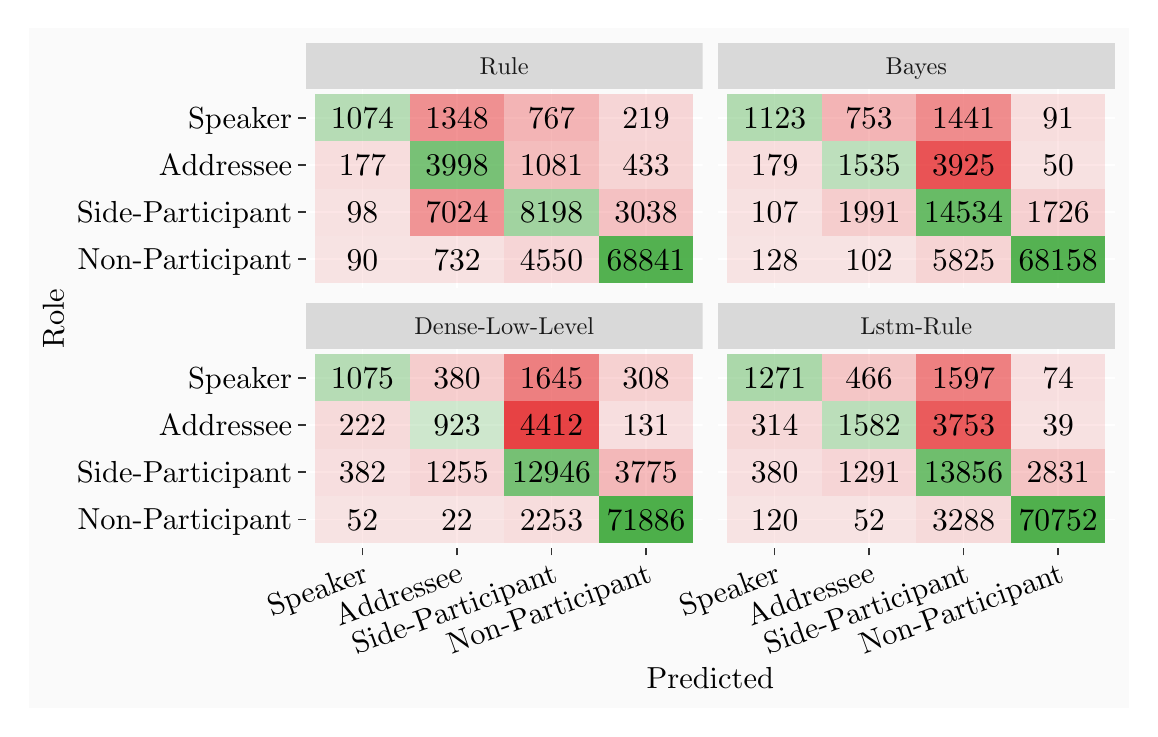
\begin{tikzpicture}[x=1pt,y=1pt]
\definecolor{fillColor}{RGB}{255,255,255}
\path[use as bounding box,fill=fillColor,fill opacity=0.00] (0,0) rectangle (398.34,246.17);
\begin{scope}
\path[clip] (  0.00,  0.00) rectangle (398.34,246.17);
\definecolor{drawColor}{RGB}{255,255,255}
\definecolor{fillColor}{gray}{0.98}

\path[draw=drawColor,line width= 0.6pt,line join=round,line cap=round,fill=fillColor] (  0.00,  0.00) rectangle (398.34,246.17);
\end{scope}
\begin{scope}
\path[clip] (100.50,152.22) rectangle (243.92,223.87);
\definecolor{drawColor}{RGB}{255,255,255}

\path[draw=drawColor,line width= 0.6pt,line join=round] (100.50,162.46) --
	(243.92,162.46);

\path[draw=drawColor,line width= 0.6pt,line join=round] (100.50,179.51) --
	(243.92,179.51);

\path[draw=drawColor,line width= 0.6pt,line join=round] (100.50,196.57) --
	(243.92,196.57);

\path[draw=drawColor,line width= 0.6pt,line join=round] (100.50,213.63) --
	(243.92,213.63);

\path[draw=drawColor,line width= 0.6pt,line join=round] (120.98,152.22) --
	(120.98,223.87);

\path[draw=drawColor,line width= 0.6pt,line join=round] (155.13,152.22) --
	(155.13,223.87);

\path[draw=drawColor,line width= 0.6pt,line join=round] (189.28,152.22) --
	(189.28,223.87);

\path[draw=drawColor,line width= 0.6pt,line join=round] (223.43,152.22) --
	(223.43,223.87);
\definecolor{fillColor}{RGB}{77,175,74}

\path[fill=fillColor,fill opacity=0.39] (103.91,205.10) rectangle (138.06,222.16);
\definecolor{fillColor}{RGB}{228,26,28}

\path[fill=fillColor,fill opacity=0.47] (138.06,205.10) rectangle (172.21,222.16);
\definecolor{fillColor}{RGB}{228,26,28}

\path[fill=fillColor,fill opacity=0.31] (172.21,205.10) rectangle (206.35,222.16);
\definecolor{fillColor}{RGB}{228,26,28}

\path[fill=fillColor,fill opacity=0.16] (206.35,205.10) rectangle (240.50,222.16);
\definecolor{fillColor}{RGB}{228,26,28}

\path[fill=fillColor,fill opacity=0.13] (103.91,188.04) rectangle (138.06,205.10);
\definecolor{fillColor}{RGB}{77,175,74}

\path[fill=fillColor,fill opacity=0.75] (138.06,188.04) rectangle (172.21,205.10);
\definecolor{fillColor}{RGB}{228,26,28}

\path[fill=fillColor,fill opacity=0.27] (172.21,188.04) rectangle (206.35,205.10);
\definecolor{fillColor}{RGB}{228,26,28}

\path[fill=fillColor,fill opacity=0.17] (206.35,188.04) rectangle (240.50,205.10);
\definecolor{fillColor}{RGB}{228,26,28}

\path[fill=fillColor,fill opacity=0.11] (103.91,170.99) rectangle (138.06,188.04);
\definecolor{fillColor}{RGB}{228,26,28}

\path[fill=fillColor,fill opacity=0.45] (138.06,170.99) rectangle (172.21,188.04);
\definecolor{fillColor}{RGB}{77,175,74}

\path[fill=fillColor,fill opacity=0.51] (172.21,170.99) rectangle (206.35,188.04);
\definecolor{fillColor}{RGB}{228,26,28}

\path[fill=fillColor,fill opacity=0.25] (206.35,170.99) rectangle (240.50,188.04);
\definecolor{fillColor}{RGB}{228,26,28}

\path[fill=fillColor,fill opacity=0.10] (103.91,153.93) rectangle (138.06,170.99);
\definecolor{fillColor}{RGB}{228,26,28}

\path[fill=fillColor,fill opacity=0.11] (138.06,153.93) rectangle (172.21,170.99);
\definecolor{fillColor}{RGB}{228,26,28}

\path[fill=fillColor,fill opacity=0.16] (172.21,153.93) rectangle (206.35,170.99);
\definecolor{fillColor}{RGB}{77,175,74}

\path[fill=fillColor,fill opacity=0.96] (206.35,153.93) rectangle (240.50,170.99);
\definecolor{drawColor}{RGB}{0,0,0}

\node[text=drawColor,anchor=base,inner sep=0pt, outer sep=0pt, scale=  1.14] at (120.98,209.71) {1074};

\node[text=drawColor,anchor=base,inner sep=0pt, outer sep=0pt, scale=  1.14] at (155.13,209.71) {1348};

\node[text=drawColor,anchor=base,inner sep=0pt, outer sep=0pt, scale=  1.14] at (189.28,209.71) {767};

\node[text=drawColor,anchor=base,inner sep=0pt, outer sep=0pt, scale=  1.14] at (223.43,209.71) {219};

\node[text=drawColor,anchor=base,inner sep=0pt, outer sep=0pt, scale=  1.14] at (120.98,192.66) {177};

\node[text=drawColor,anchor=base,inner sep=0pt, outer sep=0pt, scale=  1.14] at (155.13,192.66) {3998};

\node[text=drawColor,anchor=base,inner sep=0pt, outer sep=0pt, scale=  1.14] at (189.28,192.66) {1081};

\node[text=drawColor,anchor=base,inner sep=0pt, outer sep=0pt, scale=  1.14] at (223.43,192.66) {433};

\node[text=drawColor,anchor=base,inner sep=0pt, outer sep=0pt, scale=  1.14] at (120.98,175.60) {98};

\node[text=drawColor,anchor=base,inner sep=0pt, outer sep=0pt, scale=  1.14] at (155.13,175.60) {7024};

\node[text=drawColor,anchor=base,inner sep=0pt, outer sep=0pt, scale=  1.14] at (189.28,175.60) {8198};

\node[text=drawColor,anchor=base,inner sep=0pt, outer sep=0pt, scale=  1.14] at (223.43,175.60) {3038};

\node[text=drawColor,anchor=base,inner sep=0pt, outer sep=0pt, scale=  1.14] at (120.98,158.54) {90};

\node[text=drawColor,anchor=base,inner sep=0pt, outer sep=0pt, scale=  1.14] at (155.13,158.54) {732};

\node[text=drawColor,anchor=base,inner sep=0pt, outer sep=0pt, scale=  1.14] at (189.28,158.54) {4550};

\node[text=drawColor,anchor=base,inner sep=0pt, outer sep=0pt, scale=  1.14] at (223.43,158.54) {68841};
\end{scope}
\begin{scope}
\path[clip] (100.50, 58.27) rectangle (243.92,129.92);
\definecolor{drawColor}{RGB}{255,255,255}

\path[draw=drawColor,line width= 0.6pt,line join=round] (100.50, 68.50) --
	(243.92, 68.50);

\path[draw=drawColor,line width= 0.6pt,line join=round] (100.50, 85.56) --
	(243.92, 85.56);

\path[draw=drawColor,line width= 0.6pt,line join=round] (100.50,102.62) --
	(243.92,102.62);

\path[draw=drawColor,line width= 0.6pt,line join=round] (100.50,119.68) --
	(243.92,119.68);

\path[draw=drawColor,line width= 0.6pt,line join=round] (120.98, 58.27) --
	(120.98,129.92);

\path[draw=drawColor,line width= 0.6pt,line join=round] (155.13, 58.27) --
	(155.13,129.92);

\path[draw=drawColor,line width= 0.6pt,line join=round] (189.28, 58.27) --
	(189.28,129.92);

\path[draw=drawColor,line width= 0.6pt,line join=round] (223.43, 58.27) --
	(223.43,129.92);
\definecolor{fillColor}{RGB}{77,175,74}

\path[fill=fillColor,fill opacity=0.39] (103.91,111.15) rectangle (138.06,128.21);
\definecolor{fillColor}{RGB}{228,26,28}

\path[fill=fillColor,fill opacity=0.20] (138.06,111.15) rectangle (172.21,128.21);
\definecolor{fillColor}{RGB}{228,26,28}

\path[fill=fillColor,fill opacity=0.55] (172.21,111.15) rectangle (206.35,128.21);
\definecolor{fillColor}{RGB}{228,26,28}

\path[fill=fillColor,fill opacity=0.18] (206.35,111.15) rectangle (240.50,128.21);
\definecolor{fillColor}{RGB}{228,26,28}

\path[fill=fillColor,fill opacity=0.14] (103.91, 94.09) rectangle (138.06,111.15);
\definecolor{fillColor}{RGB}{77,175,74}

\path[fill=fillColor,fill opacity=0.25] (138.06, 94.09) rectangle (172.21,111.15);
\definecolor{fillColor}{RGB}{228,26,28}

\path[fill=fillColor,fill opacity=0.82] (172.21, 94.09) rectangle (206.35,111.15);
\definecolor{fillColor}{RGB}{228,26,28}

\path[fill=fillColor,fill opacity=0.12] (206.35, 94.09) rectangle (240.50,111.15);
\definecolor{fillColor}{RGB}{228,26,28}

\path[fill=fillColor,fill opacity=0.12] (103.91, 77.03) rectangle (138.06, 94.09);
\definecolor{fillColor}{RGB}{228,26,28}

\path[fill=fillColor,fill opacity=0.16] (138.06, 77.03) rectangle (172.21, 94.09);
\definecolor{fillColor}{RGB}{77,175,74}

\path[fill=fillColor,fill opacity=0.76] (172.21, 77.03) rectangle (206.35, 94.09);
\definecolor{fillColor}{RGB}{228,26,28}

\path[fill=fillColor,fill opacity=0.29] (206.35, 77.03) rectangle (240.50, 94.09);
\definecolor{fillColor}{RGB}{228,26,28}

\path[fill=fillColor,fill opacity=0.10] (103.91, 59.97) rectangle (138.06, 77.03);

\path[fill=fillColor,fill opacity=0.10] (138.06, 59.97) rectangle (172.21, 77.03);
\definecolor{fillColor}{RGB}{228,26,28}

\path[fill=fillColor,fill opacity=0.13] (172.21, 59.97) rectangle (206.35, 77.03);
\definecolor{fillColor}{RGB}{77,175,74}

\path[fill=fillColor] (206.35, 59.97) rectangle (240.50, 77.03);
\definecolor{drawColor}{RGB}{0,0,0}

\node[text=drawColor,anchor=base,inner sep=0pt, outer sep=0pt, scale=  1.14] at (120.98,115.76) {1075};

\node[text=drawColor,anchor=base,inner sep=0pt, outer sep=0pt, scale=  1.14] at (155.13,115.76) {380};

\node[text=drawColor,anchor=base,inner sep=0pt, outer sep=0pt, scale=  1.14] at (189.28,115.76) {1645};

\node[text=drawColor,anchor=base,inner sep=0pt, outer sep=0pt, scale=  1.14] at (223.43,115.76) {308};

\node[text=drawColor,anchor=base,inner sep=0pt, outer sep=0pt, scale=  1.14] at (120.98, 98.70) {222};

\node[text=drawColor,anchor=base,inner sep=0pt, outer sep=0pt, scale=  1.14] at (155.13, 98.70) {923};

\node[text=drawColor,anchor=base,inner sep=0pt, outer sep=0pt, scale=  1.14] at (189.28, 98.70) {4412};

\node[text=drawColor,anchor=base,inner sep=0pt, outer sep=0pt, scale=  1.14] at (223.43, 98.70) {131};

\node[text=drawColor,anchor=base,inner sep=0pt, outer sep=0pt, scale=  1.14] at (120.98, 81.64) {382};

\node[text=drawColor,anchor=base,inner sep=0pt, outer sep=0pt, scale=  1.14] at (155.13, 81.64) {1255};

\node[text=drawColor,anchor=base,inner sep=0pt, outer sep=0pt, scale=  1.14] at (189.28, 81.64) {12946};

\node[text=drawColor,anchor=base,inner sep=0pt, outer sep=0pt, scale=  1.14] at (223.43, 81.64) {3775};

\node[text=drawColor,anchor=base,inner sep=0pt, outer sep=0pt, scale=  1.14] at (120.98, 64.58) {52};

\node[text=drawColor,anchor=base,inner sep=0pt, outer sep=0pt, scale=  1.14] at (155.13, 64.58) {22};

\node[text=drawColor,anchor=base,inner sep=0pt, outer sep=0pt, scale=  1.14] at (189.28, 64.58) {2253};

\node[text=drawColor,anchor=base,inner sep=0pt, outer sep=0pt, scale=  1.14] at (223.43, 64.58) {71886};
\end{scope}
\begin{scope}
\path[clip] (249.42,152.22) rectangle (392.84,223.87);
\definecolor{drawColor}{RGB}{255,255,255}

\path[draw=drawColor,line width= 0.6pt,line join=round] (249.42,162.46) --
	(392.84,162.46);

\path[draw=drawColor,line width= 0.6pt,line join=round] (249.42,179.51) --
	(392.84,179.51);

\path[draw=drawColor,line width= 0.6pt,line join=round] (249.42,196.57) --
	(392.84,196.57);

\path[draw=drawColor,line width= 0.6pt,line join=round] (249.42,213.63) --
	(392.84,213.63);

\path[draw=drawColor,line width= 0.6pt,line join=round] (269.91,152.22) --
	(269.91,223.87);

\path[draw=drawColor,line width= 0.6pt,line join=round] (304.05,152.22) --
	(304.05,223.87);

\path[draw=drawColor,line width= 0.6pt,line join=round] (338.20,152.22) --
	(338.20,223.87);

\path[draw=drawColor,line width= 0.6pt,line join=round] (372.35,152.22) --
	(372.35,223.87);
\definecolor{fillColor}{RGB}{77,175,74}

\path[fill=fillColor,fill opacity=0.41] (252.83,205.10) rectangle (286.98,222.16);
\definecolor{fillColor}{RGB}{228,26,28}

\path[fill=fillColor,fill opacity=0.31] (286.98,205.10) rectangle (321.13,222.16);
\definecolor{fillColor}{RGB}{228,26,28}

\path[fill=fillColor,fill opacity=0.49] (321.13,205.10) rectangle (355.28,222.16);
\definecolor{fillColor}{RGB}{228,26,28}

\path[fill=fillColor,fill opacity=0.13] (355.28,205.10) rectangle (389.42,222.16);
\definecolor{fillColor}{RGB}{228,26,28}

\path[fill=fillColor,fill opacity=0.13] (252.83,188.04) rectangle (286.98,205.10);
\definecolor{fillColor}{RGB}{77,175,74}

\path[fill=fillColor,fill opacity=0.35] (286.98,188.04) rectangle (321.13,205.10);
\definecolor{fillColor}{RGB}{228,26,28}

\path[fill=fillColor,fill opacity=0.74] (321.13,188.04) rectangle (355.28,205.10);
\definecolor{fillColor}{RGB}{228,26,28}

\path[fill=fillColor,fill opacity=0.11] (355.28,188.04) rectangle (389.42,205.10);
\definecolor{fillColor}{RGB}{228,26,28}

\path[fill=fillColor,fill opacity=0.11] (252.83,170.99) rectangle (286.98,188.04);
\definecolor{fillColor}{RGB}{228,26,28}

\path[fill=fillColor,fill opacity=0.20] (286.98,170.99) rectangle (321.13,188.04);
\definecolor{fillColor}{RGB}{77,175,74}

\path[fill=fillColor,fill opacity=0.84] (321.13,170.99) rectangle (355.28,188.04);
\definecolor{fillColor}{RGB}{228,26,28}

\path[fill=fillColor,fill opacity=0.19] (355.28,170.99) rectangle (389.42,188.04);
\definecolor{fillColor}{RGB}{228,26,28}

\path[fill=fillColor,fill opacity=0.10] (252.83,153.93) rectangle (286.98,170.99);

\path[fill=fillColor,fill opacity=0.10] (286.98,153.93) rectangle (321.13,170.99);
\definecolor{fillColor}{RGB}{228,26,28}

\path[fill=fillColor,fill opacity=0.17] (321.13,153.93) rectangle (355.28,170.99);
\definecolor{fillColor}{RGB}{77,175,74}

\path[fill=fillColor,fill opacity=0.95] (355.28,153.93) rectangle (389.42,170.99);
\definecolor{drawColor}{RGB}{0,0,0}

\node[text=drawColor,anchor=base,inner sep=0pt, outer sep=0pt, scale=  1.14] at (269.91,209.71) {1123};

\node[text=drawColor,anchor=base,inner sep=0pt, outer sep=0pt, scale=  1.14] at (304.05,209.71) {753};

\node[text=drawColor,anchor=base,inner sep=0pt, outer sep=0pt, scale=  1.14] at (338.20,209.71) {1441};

\node[text=drawColor,anchor=base,inner sep=0pt, outer sep=0pt, scale=  1.14] at (372.35,209.71) {91};

\node[text=drawColor,anchor=base,inner sep=0pt, outer sep=0pt, scale=  1.14] at (269.91,192.66) {179};

\node[text=drawColor,anchor=base,inner sep=0pt, outer sep=0pt, scale=  1.14] at (304.05,192.66) {1535};

\node[text=drawColor,anchor=base,inner sep=0pt, outer sep=0pt, scale=  1.14] at (338.20,192.66) {3925};

\node[text=drawColor,anchor=base,inner sep=0pt, outer sep=0pt, scale=  1.14] at (372.35,192.66) {50};

\node[text=drawColor,anchor=base,inner sep=0pt, outer sep=0pt, scale=  1.14] at (269.91,175.60) {107};

\node[text=drawColor,anchor=base,inner sep=0pt, outer sep=0pt, scale=  1.14] at (304.05,175.60) {1991};

\node[text=drawColor,anchor=base,inner sep=0pt, outer sep=0pt, scale=  1.14] at (338.20,175.60) {14534};

\node[text=drawColor,anchor=base,inner sep=0pt, outer sep=0pt, scale=  1.14] at (372.35,175.60) {1726};

\node[text=drawColor,anchor=base,inner sep=0pt, outer sep=0pt, scale=  1.14] at (269.91,158.54) {128};

\node[text=drawColor,anchor=base,inner sep=0pt, outer sep=0pt, scale=  1.14] at (304.05,158.54) {102};

\node[text=drawColor,anchor=base,inner sep=0pt, outer sep=0pt, scale=  1.14] at (338.20,158.54) {5825};

\node[text=drawColor,anchor=base,inner sep=0pt, outer sep=0pt, scale=  1.14] at (372.35,158.54) {68158};
\end{scope}
\begin{scope}
\path[clip] (249.42, 58.27) rectangle (392.84,129.92);
\definecolor{drawColor}{RGB}{255,255,255}

\path[draw=drawColor,line width= 0.6pt,line join=round] (249.42, 68.50) --
	(392.84, 68.50);

\path[draw=drawColor,line width= 0.6pt,line join=round] (249.42, 85.56) --
	(392.84, 85.56);

\path[draw=drawColor,line width= 0.6pt,line join=round] (249.42,102.62) --
	(392.84,102.62);

\path[draw=drawColor,line width= 0.6pt,line join=round] (249.42,119.68) --
	(392.84,119.68);

\path[draw=drawColor,line width= 0.6pt,line join=round] (269.91, 58.27) --
	(269.91,129.92);

\path[draw=drawColor,line width= 0.6pt,line join=round] (304.05, 58.27) --
	(304.05,129.92);

\path[draw=drawColor,line width= 0.6pt,line join=round] (338.20, 58.27) --
	(338.20,129.92);

\path[draw=drawColor,line width= 0.6pt,line join=round] (372.35, 58.27) --
	(372.35,129.92);
\definecolor{fillColor}{RGB}{77,175,74}

\path[fill=fillColor,fill opacity=0.45] (252.83,111.15) rectangle (286.98,128.21);
\definecolor{fillColor}{RGB}{228,26,28}

\path[fill=fillColor,fill opacity=0.23] (286.98,111.15) rectangle (321.13,128.21);
\definecolor{fillColor}{RGB}{228,26,28}

\path[fill=fillColor,fill opacity=0.54] (321.13,111.15) rectangle (355.28,128.21);
\definecolor{fillColor}{RGB}{228,26,28}

\path[fill=fillColor,fill opacity=0.12] (355.28,111.15) rectangle (389.42,128.21);
\definecolor{fillColor}{RGB}{228,26,28}

\path[fill=fillColor,fill opacity=0.15] (252.83, 94.09) rectangle (286.98,111.15);
\definecolor{fillColor}{RGB}{77,175,74}

\path[fill=fillColor,fill opacity=0.36] (286.98, 94.09) rectangle (321.13,111.15);
\definecolor{fillColor}{RGB}{228,26,28}

\path[fill=fillColor,fill opacity=0.71] (321.13, 94.09) rectangle (355.28,111.15);
\definecolor{fillColor}{RGB}{228,26,28}

\path[fill=fillColor,fill opacity=0.11] (355.28, 94.09) rectangle (389.42,111.15);
\definecolor{fillColor}{RGB}{228,26,28}

\path[fill=fillColor,fill opacity=0.12] (252.83, 77.03) rectangle (286.98, 94.09);
\definecolor{fillColor}{RGB}{228,26,28}

\path[fill=fillColor,fill opacity=0.16] (286.98, 77.03) rectangle (321.13, 94.09);
\definecolor{fillColor}{RGB}{77,175,74}

\path[fill=fillColor,fill opacity=0.80] (321.13, 77.03) rectangle (355.28, 94.09);
\definecolor{fillColor}{RGB}{228,26,28}

\path[fill=fillColor,fill opacity=0.24] (355.28, 77.03) rectangle (389.42, 94.09);
\definecolor{fillColor}{RGB}{228,26,28}

\path[fill=fillColor,fill opacity=0.10] (252.83, 59.97) rectangle (286.98, 77.03);

\path[fill=fillColor,fill opacity=0.10] (286.98, 59.97) rectangle (321.13, 77.03);
\definecolor{fillColor}{RGB}{228,26,28}

\path[fill=fillColor,fill opacity=0.14] (321.13, 59.97) rectangle (355.28, 77.03);
\definecolor{fillColor}{RGB}{77,175,74}

\path[fill=fillColor,fill opacity=0.98] (355.28, 59.97) rectangle (389.42, 77.03);
\definecolor{drawColor}{RGB}{0,0,0}

\node[text=drawColor,anchor=base,inner sep=0pt, outer sep=0pt, scale=  1.14] at (269.91,115.76) {1271};

\node[text=drawColor,anchor=base,inner sep=0pt, outer sep=0pt, scale=  1.14] at (304.05,115.76) {466};

\node[text=drawColor,anchor=base,inner sep=0pt, outer sep=0pt, scale=  1.14] at (338.20,115.76) {1597};

\node[text=drawColor,anchor=base,inner sep=0pt, outer sep=0pt, scale=  1.14] at (372.35,115.76) {74};

\node[text=drawColor,anchor=base,inner sep=0pt, outer sep=0pt, scale=  1.14] at (269.91, 98.70) {314};

\node[text=drawColor,anchor=base,inner sep=0pt, outer sep=0pt, scale=  1.14] at (304.05, 98.70) {1582};

\node[text=drawColor,anchor=base,inner sep=0pt, outer sep=0pt, scale=  1.14] at (338.20, 98.70) {3753};

\node[text=drawColor,anchor=base,inner sep=0pt, outer sep=0pt, scale=  1.14] at (372.35, 98.70) {39};

\node[text=drawColor,anchor=base,inner sep=0pt, outer sep=0pt, scale=  1.14] at (269.91, 81.64) {380};

\node[text=drawColor,anchor=base,inner sep=0pt, outer sep=0pt, scale=  1.14] at (304.05, 81.64) {1291};

\node[text=drawColor,anchor=base,inner sep=0pt, outer sep=0pt, scale=  1.14] at (338.20, 81.64) {13856};

\node[text=drawColor,anchor=base,inner sep=0pt, outer sep=0pt, scale=  1.14] at (372.35, 81.64) {2831};

\node[text=drawColor,anchor=base,inner sep=0pt, outer sep=0pt, scale=  1.14] at (269.91, 64.58) {120};

\node[text=drawColor,anchor=base,inner sep=0pt, outer sep=0pt, scale=  1.14] at (304.05, 64.58) {52};

\node[text=drawColor,anchor=base,inner sep=0pt, outer sep=0pt, scale=  1.14] at (338.20, 64.58) {3288};

\node[text=drawColor,anchor=base,inner sep=0pt, outer sep=0pt, scale=  1.14] at (372.35, 64.58) {70752};
\end{scope}
\begin{scope}
\path[clip] (100.50,129.92) rectangle (243.92,146.72);
\definecolor{fillColor}{gray}{0.85}

\path[fill=fillColor] (100.50,129.92) rectangle (243.92,146.72);
\definecolor{drawColor}{gray}{0.10}

\node[text=drawColor,anchor=base,inner sep=0pt, outer sep=0pt, scale=  0.88] at (172.21,135.29) {Dense-Low-Level};
\end{scope}
\begin{scope}
\path[clip] (249.42,129.92) rectangle (392.84,146.72);
\definecolor{fillColor}{gray}{0.85}

\path[fill=fillColor] (249.42,129.92) rectangle (392.84,146.72);
\definecolor{drawColor}{gray}{0.10}

\node[text=drawColor,anchor=base,inner sep=0pt, outer sep=0pt, scale=  0.88] at (321.13,135.29) {Lstm-Rule};
\end{scope}
\begin{scope}
\path[clip] (100.50,223.87) rectangle (243.92,240.67);
\definecolor{fillColor}{gray}{0.85}

\path[fill=fillColor] (100.50,223.87) rectangle (243.92,240.67);
\definecolor{drawColor}{gray}{0.10}

\node[text=drawColor,anchor=base,inner sep=0pt, outer sep=0pt, scale=  0.88] at (172.21,229.24) {Rule};
\end{scope}
\begin{scope}
\path[clip] (249.42,223.87) rectangle (392.84,240.67);
\definecolor{fillColor}{gray}{0.85}

\path[fill=fillColor] (249.42,223.87) rectangle (392.84,240.67);
\definecolor{drawColor}{gray}{0.10}

\node[text=drawColor,anchor=base,inner sep=0pt, outer sep=0pt, scale=  0.88] at (321.13,229.24) {Bayes};
\end{scope}
\begin{scope}
\path[clip] (  0.00,  0.00) rectangle (398.34,246.17);
\definecolor{drawColor}{gray}{0.20}

\path[draw=drawColor,line width= 0.6pt,line join=round] (120.98, 55.52) --
	(120.98, 58.27);

\path[draw=drawColor,line width= 0.6pt,line join=round] (155.13, 55.52) --
	(155.13, 58.27);

\path[draw=drawColor,line width= 0.6pt,line join=round] (189.28, 55.52) --
	(189.28, 58.27);

\path[draw=drawColor,line width= 0.6pt,line join=round] (223.43, 55.52) --
	(223.43, 58.27);
\end{scope}
\begin{scope}
\path[clip] (  0.00,  0.00) rectangle (398.34,246.17);
\definecolor{drawColor}{RGB}{0,0,0}

\node[text=drawColor,rotate= 20.00,anchor=base east,inner sep=0pt, outer sep=0pt, scale=  1.10] at (123.58, 46.20) {Speaker};

\node[text=drawColor,rotate= 20.00,anchor=base east,inner sep=0pt, outer sep=0pt, scale=  1.10] at (157.72, 46.20) {Addressee};

\node[text=drawColor,rotate= 20.00,anchor=base east,inner sep=0pt, outer sep=0pt, scale=  1.10] at (191.87, 46.20) {Side-Participant};

\node[text=drawColor,rotate= 20.00,anchor=base east,inner sep=0pt, outer sep=0pt, scale=  1.10] at (226.02, 46.20) {Non-Participant};
\end{scope}
\begin{scope}
\path[clip] (  0.00,  0.00) rectangle (398.34,246.17);
\definecolor{drawColor}{gray}{0.20}

\path[draw=drawColor,line width= 0.6pt,line join=round] (269.91, 55.52) --
	(269.91, 58.27);

\path[draw=drawColor,line width= 0.6pt,line join=round] (304.05, 55.52) --
	(304.05, 58.27);

\path[draw=drawColor,line width= 0.6pt,line join=round] (338.20, 55.52) --
	(338.20, 58.27);

\path[draw=drawColor,line width= 0.6pt,line join=round] (372.35, 55.52) --
	(372.35, 58.27);
\end{scope}
\begin{scope}
\path[clip] (  0.00,  0.00) rectangle (398.34,246.17);
\definecolor{drawColor}{RGB}{0,0,0}

\node[text=drawColor,rotate= 20.00,anchor=base east,inner sep=0pt, outer sep=0pt, scale=  1.10] at (272.50, 46.20) {Speaker};

\node[text=drawColor,rotate= 20.00,anchor=base east,inner sep=0pt, outer sep=0pt, scale=  1.10] at (306.65, 46.20) {Addressee};

\node[text=drawColor,rotate= 20.00,anchor=base east,inner sep=0pt, outer sep=0pt, scale=  1.10] at (340.79, 46.20) {Side-Participant};

\node[text=drawColor,rotate= 20.00,anchor=base east,inner sep=0pt, outer sep=0pt, scale=  1.10] at (374.94, 46.20) {Non-Participant};
\end{scope}
\begin{scope}
\path[clip] (  0.00,  0.00) rectangle (398.34,246.17);
\definecolor{drawColor}{RGB}{0,0,0}

\node[text=drawColor,anchor=base east,inner sep=0pt, outer sep=0pt, scale=  1.10] at ( 95.55,158.67) {Non-Participant};

\node[text=drawColor,anchor=base east,inner sep=0pt, outer sep=0pt, scale=  1.10] at ( 95.55,175.73) {Side-Participant};

\node[text=drawColor,anchor=base east,inner sep=0pt, outer sep=0pt, scale=  1.10] at ( 95.55,192.79) {Addressee};

\node[text=drawColor,anchor=base east,inner sep=0pt, outer sep=0pt, scale=  1.10] at ( 95.55,209.85) {Speaker};
\end{scope}
\begin{scope}
\path[clip] (  0.00,  0.00) rectangle (398.34,246.17);
\definecolor{drawColor}{gray}{0.20}

\path[draw=drawColor,line width= 0.6pt,line join=round] ( 97.75,162.46) --
	(100.50,162.46);

\path[draw=drawColor,line width= 0.6pt,line join=round] ( 97.75,179.51) --
	(100.50,179.51);

\path[draw=drawColor,line width= 0.6pt,line join=round] ( 97.75,196.57) --
	(100.50,196.57);

\path[draw=drawColor,line width= 0.6pt,line join=round] ( 97.75,213.63) --
	(100.50,213.63);
\end{scope}
\begin{scope}
\path[clip] (  0.00,  0.00) rectangle (398.34,246.17);
\definecolor{drawColor}{RGB}{0,0,0}

\node[text=drawColor,anchor=base east,inner sep=0pt, outer sep=0pt, scale=  1.10] at ( 95.55, 64.71) {Non-Participant};

\node[text=drawColor,anchor=base east,inner sep=0pt, outer sep=0pt, scale=  1.10] at ( 95.55, 81.77) {Side-Participant};

\node[text=drawColor,anchor=base east,inner sep=0pt, outer sep=0pt, scale=  1.10] at ( 95.55, 98.83) {Addressee};

\node[text=drawColor,anchor=base east,inner sep=0pt, outer sep=0pt, scale=  1.10] at ( 95.55,115.89) {Speaker};
\end{scope}
\begin{scope}
\path[clip] (  0.00,  0.00) rectangle (398.34,246.17);
\definecolor{drawColor}{gray}{0.20}

\path[draw=drawColor,line width= 0.6pt,line join=round] ( 97.75, 68.50) --
	(100.50, 68.50);

\path[draw=drawColor,line width= 0.6pt,line join=round] ( 97.75, 85.56) --
	(100.50, 85.56);

\path[draw=drawColor,line width= 0.6pt,line join=round] ( 97.75,102.62) --
	(100.50,102.62);

\path[draw=drawColor,line width= 0.6pt,line join=round] ( 97.75,119.68) --
	(100.50,119.68);
\end{scope}
\begin{scope}
\path[clip] (  0.00,  0.00) rectangle (398.34,246.17);
\definecolor{drawColor}{RGB}{0,0,0}

\node[text=drawColor,anchor=base,inner sep=0pt, outer sep=0pt, scale=  1.10] at (246.67,  7.44) {Predicted};
\end{scope}
\begin{scope}
\path[clip] (  0.00,  0.00) rectangle (398.34,246.17);
\definecolor{drawColor}{RGB}{0,0,0}

\node[text=drawColor,rotate= 90.00,anchor=base,inner sep=0pt, outer sep=0pt, scale=  1.10] at ( 13.08,141.07) {Role};
\end{scope}
\end{tikzpicture}

    }
\end{frame}
\begin{frame}{Results - Simple Models}
  \begin{columns}[T] % align columns
    \begin{column}{.7\textwidth}
      \resizebox{1.\textwidth}{!}{%
        \scriptsize
        \begin{tikzpicture}
          \node (b) at (0,0)
          {
            \resizebox{\textwidth}{!}{%
            % Created by tikzDevice version 0.12
% !TEX encoding = UTF-8 Unicode
\begin{tikzpicture}[x=1pt,y=1pt]
\definecolor{fillColor}{RGB}{255,255,255}
\path[use as bounding box,fill=fillColor,fill opacity=0.00] (0,0) rectangle (398.34,246.17);
\begin{scope}
\path[clip] (  0.00, 11.30) rectangle (398.34,234.87);
\definecolor{drawColor}{RGB}{255,255,255}
\definecolor{fillColor}{gray}{0.98}

\path[draw=drawColor,line width= 0.6pt,line join=round,line cap=round,fill=fillColor] (  0.00, 11.30) rectangle (398.34,234.87);
\end{scope}
\begin{scope}
\path[clip] ( 92.74, 65.82) rectangle (240.04,213.12);
\definecolor{drawColor}{RGB}{255,255,255}

\path[draw=drawColor,line width= 0.6pt,line join=round] ( 92.74, 86.86) --
	(240.04, 86.86);

\path[draw=drawColor,line width= 0.6pt,line join=round] ( 92.74,121.93) --
	(240.04,121.93);

\path[draw=drawColor,line width= 0.6pt,line join=round] ( 92.74,157.00) --
	(240.04,157.00);

\path[draw=drawColor,line width= 0.6pt,line join=round] ( 92.74,192.07) --
	(240.04,192.07);

\path[draw=drawColor,line width= 0.6pt,line join=round] (113.78, 65.82) --
	(113.78,213.12);

\path[draw=drawColor,line width= 0.6pt,line join=round] (148.85, 65.82) --
	(148.85,213.12);

\path[draw=drawColor,line width= 0.6pt,line join=round] (183.92, 65.82) --
	(183.92,213.12);

\path[draw=drawColor,line width= 0.6pt,line join=round] (218.99, 65.82) --
	(218.99,213.12);
\definecolor{fillColor}{RGB}{77,175,74}

\path[fill=fillColor,fill opacity=0.40] ( 96.24,174.54) rectangle (131.32,209.61);
\definecolor{fillColor}{RGB}{228,26,28}

\path[fill=fillColor,fill opacity=0.48] (131.32,174.54) rectangle (166.39,209.61);
\definecolor{fillColor}{RGB}{228,26,28}

\path[fill=fillColor,fill opacity=0.32] (166.39,174.54) rectangle (201.46,209.61);
\definecolor{fillColor}{RGB}{228,26,28}

\path[fill=fillColor,fill opacity=0.16] (201.46,174.54) rectangle (236.53,209.61);
\definecolor{fillColor}{RGB}{228,26,28}

\path[fill=fillColor,fill opacity=0.13] ( 96.24,139.47) rectangle (131.32,174.54);
\definecolor{fillColor}{RGB}{77,175,74}

\path[fill=fillColor,fill opacity=0.78] (131.32,139.47) rectangle (166.39,174.54);
\definecolor{fillColor}{RGB}{228,26,28}

\path[fill=fillColor,fill opacity=0.28] (166.39,139.47) rectangle (201.46,174.54);
\definecolor{fillColor}{RGB}{228,26,28}

\path[fill=fillColor,fill opacity=0.17] (201.46,139.47) rectangle (236.53,174.54);
\definecolor{fillColor}{RGB}{228,26,28}

\path[fill=fillColor,fill opacity=0.11] ( 96.24,104.39) rectangle (131.32,139.47);
\definecolor{fillColor}{RGB}{228,26,28}

\path[fill=fillColor,fill opacity=0.47] (131.32,104.39) rectangle (166.39,139.47);
\definecolor{fillColor}{RGB}{77,175,74}

\path[fill=fillColor,fill opacity=0.53] (166.39,104.39) rectangle (201.46,139.47);
\definecolor{fillColor}{RGB}{228,26,28}

\path[fill=fillColor,fill opacity=0.26] (201.46,104.39) rectangle (236.53,139.47);
\definecolor{fillColor}{RGB}{228,26,28}

\path[fill=fillColor,fill opacity=0.10] ( 96.24, 69.32) rectangle (131.32,104.39);
\definecolor{fillColor}{RGB}{228,26,28}

\path[fill=fillColor,fill opacity=0.11] (131.32, 69.32) rectangle (166.39,104.39);
\definecolor{fillColor}{RGB}{228,26,28}

\path[fill=fillColor,fill opacity=0.16] (166.39, 69.32) rectangle (201.46,104.39);
\definecolor{fillColor}{RGB}{77,175,74}

\path[fill=fillColor] (201.46, 69.32) rectangle (236.53,104.39);
\definecolor{drawColor}{RGB}{0,0,0}

\node[text=drawColor,anchor=base,inner sep=0pt, outer sep=0pt, scale=  1.14] at (113.78,188.15) {0.32};

\node[text=drawColor,anchor=base,inner sep=0pt, outer sep=0pt, scale=  1.14] at (148.85,188.15) {0.40};

\node[text=drawColor,anchor=base,inner sep=0pt, outer sep=0pt, scale=  1.14] at (183.92,188.15) {0.23};

\node[text=drawColor,anchor=base,inner sep=0pt, outer sep=0pt, scale=  1.14] at (218.99,188.15) {0.06};

\node[text=drawColor,anchor=base,inner sep=0pt, outer sep=0pt, scale=  1.14] at (113.78,153.08) {0.03};

\node[text=drawColor,anchor=base,inner sep=0pt, outer sep=0pt, scale=  1.14] at (148.85,153.08) {0.70};

\node[text=drawColor,anchor=base,inner sep=0pt, outer sep=0pt, scale=  1.14] at (183.92,153.08) {0.19};

\node[text=drawColor,anchor=base,inner sep=0pt, outer sep=0pt, scale=  1.14] at (218.99,153.08) {0.08};

\node[text=drawColor,anchor=base,inner sep=0pt, outer sep=0pt, scale=  1.14] at (113.78,118.01) {0.01};

\node[text=drawColor,anchor=base,inner sep=0pt, outer sep=0pt, scale=  1.14] at (148.85,118.01) {0.38};

\node[text=drawColor,anchor=base,inner sep=0pt, outer sep=0pt, scale=  1.14] at (183.92,118.01) {0.45};

\node[text=drawColor,anchor=base,inner sep=0pt, outer sep=0pt, scale=  1.14] at (218.99,118.01) {0.17};

\node[text=drawColor,anchor=base,inner sep=0pt, outer sep=0pt, scale=  1.14] at (113.78, 82.94) {0.00};

\node[text=drawColor,anchor=base,inner sep=0pt, outer sep=0pt, scale=  1.14] at (148.85, 82.94) {0.01};

\node[text=drawColor,anchor=base,inner sep=0pt, outer sep=0pt, scale=  1.14] at (183.92, 82.94) {0.06};

\node[text=drawColor,anchor=base,inner sep=0pt, outer sep=0pt, scale=  1.14] at (218.99, 82.94) {0.93};
\end{scope}
\begin{scope}
\path[clip] (245.54, 65.82) rectangle (392.84,213.12);
\definecolor{drawColor}{RGB}{255,255,255}

\path[draw=drawColor,line width= 0.6pt,line join=round] (245.54, 86.86) --
	(392.84, 86.86);

\path[draw=drawColor,line width= 0.6pt,line join=round] (245.54,121.93) --
	(392.84,121.93);

\path[draw=drawColor,line width= 0.6pt,line join=round] (245.54,157.00) --
	(392.84,157.00);

\path[draw=drawColor,line width= 0.6pt,line join=round] (245.54,192.07) --
	(392.84,192.07);

\path[draw=drawColor,line width= 0.6pt,line join=round] (266.58, 65.82) --
	(266.58,213.12);

\path[draw=drawColor,line width= 0.6pt,line join=round] (301.65, 65.82) --
	(301.65,213.12);

\path[draw=drawColor,line width= 0.6pt,line join=round] (336.72, 65.82) --
	(336.72,213.12);

\path[draw=drawColor,line width= 0.6pt,line join=round] (371.80, 65.82) --
	(371.80,213.12);
\definecolor{fillColor}{RGB}{77,175,74}

\path[fill=fillColor,fill opacity=0.42] (249.04,174.54) rectangle (284.12,209.61);
\definecolor{fillColor}{RGB}{228,26,28}

\path[fill=fillColor,fill opacity=0.31] (284.12,174.54) rectangle (319.19,209.61);
\definecolor{fillColor}{RGB}{228,26,28}

\path[fill=fillColor,fill opacity=0.51] (319.19,174.54) rectangle (354.26,209.61);
\definecolor{fillColor}{RGB}{228,26,28}

\path[fill=fillColor,fill opacity=0.13] (354.26,174.54) rectangle (389.33,209.61);
\definecolor{fillColor}{RGB}{228,26,28}

\path[fill=fillColor,fill opacity=0.13] (249.04,139.47) rectangle (284.12,174.54);
\definecolor{fillColor}{RGB}{77,175,74}

\path[fill=fillColor,fill opacity=0.36] (284.12,139.47) rectangle (319.19,174.54);
\definecolor{fillColor}{RGB}{228,26,28}

\path[fill=fillColor,fill opacity=0.77] (319.19,139.47) rectangle (354.26,174.54);
\definecolor{fillColor}{RGB}{228,26,28}

\path[fill=fillColor,fill opacity=0.11] (354.26,139.47) rectangle (389.33,174.54);

\path[fill=fillColor,fill opacity=0.11] (249.04,104.39) rectangle (284.12,139.47);
\definecolor{fillColor}{RGB}{228,26,28}

\path[fill=fillColor,fill opacity=0.20] (284.12,104.39) rectangle (319.19,139.47);
\definecolor{fillColor}{RGB}{77,175,74}

\path[fill=fillColor,fill opacity=0.87] (319.19,104.39) rectangle (354.26,139.47);
\definecolor{fillColor}{RGB}{228,26,28}

\path[fill=fillColor,fill opacity=0.19] (354.26,104.39) rectangle (389.33,139.47);
\definecolor{fillColor}{RGB}{228,26,28}

\path[fill=fillColor,fill opacity=0.10] (249.04, 69.32) rectangle (284.12,104.39);

\path[fill=fillColor,fill opacity=0.10] (284.12, 69.32) rectangle (319.19,104.39);
\definecolor{fillColor}{RGB}{228,26,28}

\path[fill=fillColor,fill opacity=0.18] (319.19, 69.32) rectangle (354.26,104.39);
\definecolor{fillColor}{RGB}{77,175,74}

\path[fill=fillColor,fill opacity=0.99] (354.26, 69.32) rectangle (389.33,104.39);
\definecolor{drawColor}{RGB}{0,0,0}

\node[text=drawColor,anchor=base,inner sep=0pt, outer sep=0pt, scale=  1.14] at (266.58,188.15) {0.33};

\node[text=drawColor,anchor=base,inner sep=0pt, outer sep=0pt, scale=  1.14] at (301.65,188.15) {0.22};

\node[text=drawColor,anchor=base,inner sep=0pt, outer sep=0pt, scale=  1.14] at (336.72,188.15) {0.42};

\node[text=drawColor,anchor=base,inner sep=0pt, outer sep=0pt, scale=  1.14] at (371.80,188.15) {0.03};

\node[text=drawColor,anchor=base,inner sep=0pt, outer sep=0pt, scale=  1.14] at (266.58,153.08) {0.03};

\node[text=drawColor,anchor=base,inner sep=0pt, outer sep=0pt, scale=  1.14] at (301.65,153.08) {0.27};

\node[text=drawColor,anchor=base,inner sep=0pt, outer sep=0pt, scale=  1.14] at (336.72,153.08) {0.69};

\node[text=drawColor,anchor=base,inner sep=0pt, outer sep=0pt, scale=  1.14] at (371.80,153.08) {0.01};

\node[text=drawColor,anchor=base,inner sep=0pt, outer sep=0pt, scale=  1.14] at (266.58,118.01) {0.01};

\node[text=drawColor,anchor=base,inner sep=0pt, outer sep=0pt, scale=  1.14] at (301.65,118.01) {0.11};

\node[text=drawColor,anchor=base,inner sep=0pt, outer sep=0pt, scale=  1.14] at (336.72,118.01) {0.79};

\node[text=drawColor,anchor=base,inner sep=0pt, outer sep=0pt, scale=  1.14] at (371.80,118.01) {0.09};

\node[text=drawColor,anchor=base,inner sep=0pt, outer sep=0pt, scale=  1.14] at (266.58, 82.94) {0.00};

\node[text=drawColor,anchor=base,inner sep=0pt, outer sep=0pt, scale=  1.14] at (301.65, 82.94) {0.00};

\node[text=drawColor,anchor=base,inner sep=0pt, outer sep=0pt, scale=  1.14] at (336.72, 82.94) {0.08};

\node[text=drawColor,anchor=base,inner sep=0pt, outer sep=0pt, scale=  1.14] at (371.80, 82.94) {0.92};
\end{scope}
\begin{scope}
\path[clip] ( 92.74,213.12) rectangle (240.04,229.37);
\definecolor{fillColor}{gray}{0.85}

\path[fill=fillColor] ( 92.74,213.12) rectangle (240.04,229.37);
\definecolor{drawColor}{gray}{0.10}

\node[text=drawColor,anchor=base,inner sep=0pt, outer sep=0pt, scale=  0.80] at (166.39,218.49) {Rule};
\end{scope}
\begin{scope}
\path[clip] (245.54,213.12) rectangle (392.84,229.37);
\definecolor{fillColor}{gray}{0.85}

\path[fill=fillColor] (245.54,213.12) rectangle (392.84,229.37);
\definecolor{drawColor}{gray}{0.10}

\node[text=drawColor,anchor=base,inner sep=0pt, outer sep=0pt, scale=  0.80] at (319.19,218.49) {Bayes};
\end{scope}
\begin{scope}
\path[clip] (  0.00,  0.00) rectangle (398.34,246.17);
\definecolor{drawColor}{gray}{0.20}

\path[draw=drawColor,line width= 0.6pt,line join=round] (113.78, 63.07) --
	(113.78, 65.82);

\path[draw=drawColor,line width= 0.6pt,line join=round] (148.85, 63.07) --
	(148.85, 65.82);

\path[draw=drawColor,line width= 0.6pt,line join=round] (183.92, 63.07) --
	(183.92, 65.82);

\path[draw=drawColor,line width= 0.6pt,line join=round] (218.99, 63.07) --
	(218.99, 65.82);
\end{scope}
\begin{scope}
\path[clip] (  0.00,  0.00) rectangle (398.34,246.17);
\definecolor{drawColor}{RGB}{0,0,0}

\node[text=drawColor,rotate= 20.00,anchor=base east,inner sep=0pt, outer sep=0pt, scale=  1.00] at (116.13, 54.39) {Speaker};

\node[text=drawColor,rotate= 20.00,anchor=base east,inner sep=0pt, outer sep=0pt, scale=  1.00] at (151.21, 54.39) {Addressee};

\node[text=drawColor,rotate= 20.00,anchor=base east,inner sep=0pt, outer sep=0pt, scale=  1.00] at (186.28, 54.39) {Side-Participant};

\node[text=drawColor,rotate= 20.00,anchor=base east,inner sep=0pt, outer sep=0pt, scale=  1.00] at (221.35, 54.39) {Non-Participant};
\end{scope}
\begin{scope}
\path[clip] (  0.00,  0.00) rectangle (398.34,246.17);
\definecolor{drawColor}{gray}{0.20}

\path[draw=drawColor,line width= 0.6pt,line join=round] (266.58, 63.07) --
	(266.58, 65.82);

\path[draw=drawColor,line width= 0.6pt,line join=round] (301.65, 63.07) --
	(301.65, 65.82);

\path[draw=drawColor,line width= 0.6pt,line join=round] (336.72, 63.07) --
	(336.72, 65.82);

\path[draw=drawColor,line width= 0.6pt,line join=round] (371.80, 63.07) --
	(371.80, 65.82);
\end{scope}
\begin{scope}
\path[clip] (  0.00,  0.00) rectangle (398.34,246.17);
\definecolor{drawColor}{RGB}{0,0,0}

\node[text=drawColor,rotate= 20.00,anchor=base east,inner sep=0pt, outer sep=0pt, scale=  1.00] at (268.94, 54.39) {Speaker};

\node[text=drawColor,rotate= 20.00,anchor=base east,inner sep=0pt, outer sep=0pt, scale=  1.00] at (304.01, 54.39) {Addressee};

\node[text=drawColor,rotate= 20.00,anchor=base east,inner sep=0pt, outer sep=0pt, scale=  1.00] at (339.08, 54.39) {Side-Participant};

\node[text=drawColor,rotate= 20.00,anchor=base east,inner sep=0pt, outer sep=0pt, scale=  1.00] at (374.15, 54.39) {Non-Participant};
\end{scope}
\begin{scope}
\path[clip] (  0.00,  0.00) rectangle (398.34,246.17);
\definecolor{drawColor}{RGB}{0,0,0}

\node[text=drawColor,anchor=base east,inner sep=0pt, outer sep=0pt, scale=  1.00] at ( 87.79, 83.41) {Non-Participant};

\node[text=drawColor,anchor=base east,inner sep=0pt, outer sep=0pt, scale=  1.00] at ( 87.79,118.49) {Side-Participant};

\node[text=drawColor,anchor=base east,inner sep=0pt, outer sep=0pt, scale=  1.00] at ( 87.79,153.56) {Addressee};

\node[text=drawColor,anchor=base east,inner sep=0pt, outer sep=0pt, scale=  1.00] at ( 87.79,188.63) {Speaker};
\end{scope}
\begin{scope}
\path[clip] (  0.00,  0.00) rectangle (398.34,246.17);
\definecolor{drawColor}{gray}{0.20}

\path[draw=drawColor,line width= 0.6pt,line join=round] ( 89.99, 86.86) --
	( 92.74, 86.86);

\path[draw=drawColor,line width= 0.6pt,line join=round] ( 89.99,121.93) --
	( 92.74,121.93);

\path[draw=drawColor,line width= 0.6pt,line join=round] ( 89.99,157.00) --
	( 92.74,157.00);

\path[draw=drawColor,line width= 0.6pt,line join=round] ( 89.99,192.07) --
	( 92.74,192.07);
\end{scope}
\begin{scope}
\path[clip] (  0.00,  0.00) rectangle (398.34,246.17);
\definecolor{drawColor}{RGB}{0,0,0}

\node[text=drawColor,anchor=base,inner sep=0pt, outer sep=0pt, scale=  1.00] at (242.79, 18.75) {Predicted};
\end{scope}
\begin{scope}
\path[clip] (  0.00,  0.00) rectangle (398.34,246.17);
\definecolor{drawColor}{RGB}{0,0,0}

\node[text=drawColor,rotate= 90.00,anchor=base,inner sep=0pt, outer sep=0pt, scale=  1.00] at ( 12.39,139.47) {Role};
\end{scope}
\end{tikzpicture}

            }
          };
          \action<1-3>{\filldraw [fill=bgcolorframe, draw=bgcolorframe] (.12\textwidth,-.125\textwidth) rectangle (.48\textwidth,.215\textwidth);}
        \end{tikzpicture}
      }
    \end{column}%
    \begin{column}{.4\textwidth}
      \vspace{10pt}
      \footnotesize
      \begin{itemize}[label=-]
        \item<1->[] Rule Model 
        \item<2-> Non-Participant good
        \item<3-> Bias for \(Addressee\)
      \end{itemize}
      \vspace{5pt}
      \begin{itemize}[label=-]
        \item<4->[] Bayes Model
        \item<4-> Non-Participant good 
        \item<5-> Bias for \(Side\text{-}Participant\)
        \item<6-> \emph{optimal} results
      \end{itemize}
      \vspace{5pt}
      \begin{itemize}[label=-]
        \item<7->[\textcolor{mygreen}{\faCheckCircle}] Simple Models
      \end{itemize}
    \end{column}%
  \end{columns}
\end{frame}
\begin{frame}{Low-Level Features \& Time Sequences}
  \begin{columns}[T] % align columns
    \begin{column}{.25\textwidth}
      \vspace{10pt}
      \centering
      \resizebox{\textwidth}{!}{%
          \scriptsize
          \begin{tikzpicture}
          \node (b) at (0,0)
          {
            \resizebox{1.35\textwidth}{!}{%
            \def\svgwidth{1.3\textwidth}
            \input{generated/nnl-defence-dense.pdf_tex}
            }
          };
          \action<6->{\node (c) at (0,-5)
          {
            \resizebox{1.35\textwidth}{!}{%
            \def\svgwidth{1.3\textwidth}
            \input{generated/nnl-defence-t2.pdf_tex}
            }
          };}
          \action<6->{\node (c) at (0,-5)
          {
            \resizebox{1.35\textwidth}{!}{%
            \def\svgwidth{1.3\textwidth}
            \input{generated/nnl-defence-t1.pdf_tex}
            }
          };}
          \action<6->{\node (c) at (0,-5)
          {
            \resizebox{1.35\textwidth}{!}{%
            \def\svgwidth{1.3\textwidth}
            \input{generated/nnl-defence-lstm.pdf_tex}
            }
          };}
           \end{tikzpicture}
        }
    \end{column}%
    \begin{column}{.75\textwidth}
    \onslide<2->{
\footnotesize\hspace{30pt}
    \begin{itemize}
      \item<2->[]Feature Sets
      \item<3->[\(Rule\)] 4D Binary, same as Bayesian Network
      \item<4->[\(Rule_{raw}\)] 4D Continuous, from underlying cost functions  
      \item<5->[\(full\)] 148D Continuous, Agent ID - Face Keypoints - Number of Persons - Group Position - Group Sub-Costs 
    \end{itemize}
    \vspace{20pt}
    \begin{itemize}
      \item<6->[]Same Feature Sets
      \item<6->[\(time\)] Time Sequences of 15 Observations \(\approx\) \SI{1}{\second}
    \end{itemize}
    }
    \end{column}%
  \end{columns}%
\end{frame}
\begin{frame}{Results - Accuracy \& Mean \(F_1\)}
  \begin{columns}[T] % align columns
    \begin{column}{.55\textwidth}
      \resizebox{1.\textwidth}{!}{%
        \small
        % Created by tikzDevice version 0.12
% !TEX encoding = UTF-8 Unicode
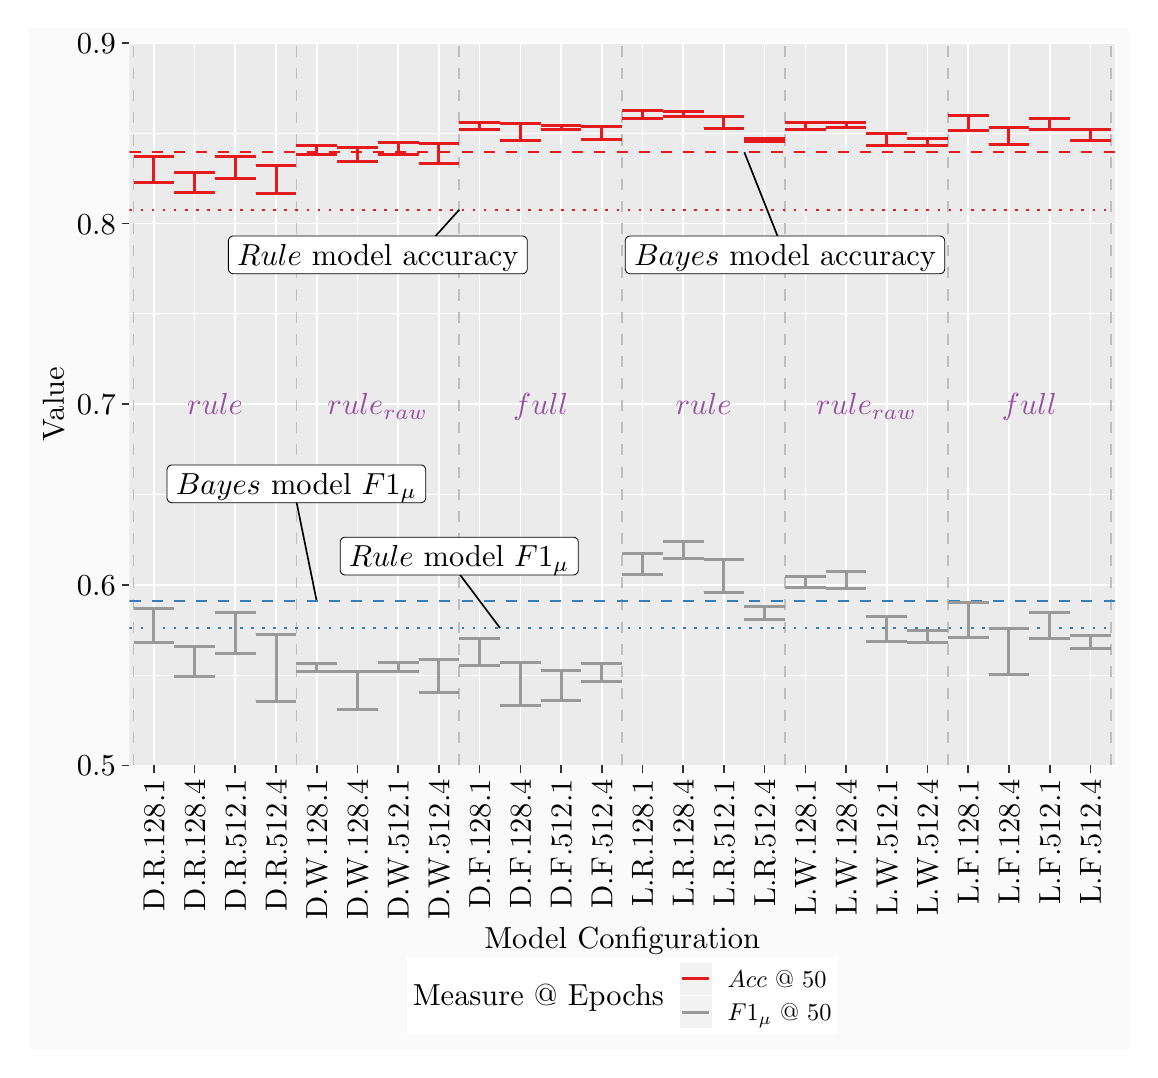
\begin{tikzpicture}[x=1pt,y=1pt]
\definecolor{fillColor}{RGB}{255,255,255}
\path[use as bounding box,fill=fillColor,fill opacity=0.00] (0,0) rectangle (398.34,369.26);
\begin{scope}
\path[clip] (  0.00,  0.00) rectangle (398.34,369.26);
\definecolor{drawColor}{RGB}{255,255,255}
\definecolor{fillColor}{gray}{0.98}

\path[draw=drawColor,line width= 0.6pt,line join=round,line cap=round,fill=fillColor] (  0.00,  0.00) rectangle (398.34,369.26);
\end{scope}
\begin{scope}
\path[clip] ( 36.77,102.67) rectangle (392.84,363.76);
\definecolor{fillColor}{gray}{0.92}

\path[fill=fillColor] ( 36.77,102.67) rectangle (392.84,363.76);
\definecolor{drawColor}{RGB}{255,255,255}

\path[draw=drawColor,line width= 0.3pt,line join=round] ( 36.77,135.31) --
	(392.84,135.31);

\path[draw=drawColor,line width= 0.3pt,line join=round] ( 36.77,200.58) --
	(392.84,200.58);

\path[draw=drawColor,line width= 0.3pt,line join=round] ( 36.77,265.85) --
	(392.84,265.85);

\path[draw=drawColor,line width= 0.3pt,line join=round] ( 36.77,331.12) --
	(392.84,331.12);

\path[draw=drawColor,line width= 0.6pt,line join=round] ( 36.77,102.67) --
	(392.84,102.67);

\path[draw=drawColor,line width= 0.6pt,line join=round] ( 36.77,167.94) --
	(392.84,167.94);

\path[draw=drawColor,line width= 0.6pt,line join=round] ( 36.77,233.22) --
	(392.84,233.22);

\path[draw=drawColor,line width= 0.6pt,line join=round] ( 36.77,298.49) --
	(392.84,298.49);

\path[draw=drawColor,line width= 0.6pt,line join=round] ( 36.77,363.76) --
	(392.84,363.76);

\path[draw=drawColor,line width= 0.6pt,line join=round] ( 45.60,102.67) --
	( 45.60,363.76);

\path[draw=drawColor,line width= 0.6pt,line join=round] ( 60.31,102.67) --
	( 60.31,363.76);

\path[draw=drawColor,line width= 0.6pt,line join=round] ( 75.03,102.67) --
	( 75.03,363.76);

\path[draw=drawColor,line width= 0.6pt,line join=round] ( 89.74,102.67) --
	( 89.74,363.76);

\path[draw=drawColor,line width= 0.6pt,line join=round] (104.45,102.67) --
	(104.45,363.76);

\path[draw=drawColor,line width= 0.6pt,line join=round] (119.17,102.67) --
	(119.17,363.76);

\path[draw=drawColor,line width= 0.6pt,line join=round] (133.88,102.67) --
	(133.88,363.76);

\path[draw=drawColor,line width= 0.6pt,line join=round] (148.59,102.67) --
	(148.59,363.76);

\path[draw=drawColor,line width= 0.6pt,line join=round] (163.31,102.67) --
	(163.31,363.76);

\path[draw=drawColor,line width= 0.6pt,line join=round] (178.02,102.67) --
	(178.02,363.76);

\path[draw=drawColor,line width= 0.6pt,line join=round] (192.74,102.67) --
	(192.74,363.76);

\path[draw=drawColor,line width= 0.6pt,line join=round] (207.45,102.67) --
	(207.45,363.76);

\path[draw=drawColor,line width= 0.6pt,line join=round] (222.16,102.67) --
	(222.16,363.76);

\path[draw=drawColor,line width= 0.6pt,line join=round] (236.88,102.67) --
	(236.88,363.76);

\path[draw=drawColor,line width= 0.6pt,line join=round] (251.59,102.67) --
	(251.59,363.76);

\path[draw=drawColor,line width= 0.6pt,line join=round] (266.30,102.67) --
	(266.30,363.76);

\path[draw=drawColor,line width= 0.6pt,line join=round] (281.02,102.67) --
	(281.02,363.76);

\path[draw=drawColor,line width= 0.6pt,line join=round] (295.73,102.67) --
	(295.73,363.76);

\path[draw=drawColor,line width= 0.6pt,line join=round] (310.44,102.67) --
	(310.44,363.76);

\path[draw=drawColor,line width= 0.6pt,line join=round] (325.16,102.67) --
	(325.16,363.76);

\path[draw=drawColor,line width= 0.6pt,line join=round] (339.87,102.67) --
	(339.87,363.76);

\path[draw=drawColor,line width= 0.6pt,line join=round] (354.58,102.67) --
	(354.58,363.76);

\path[draw=drawColor,line width= 0.6pt,line join=round] (369.30,102.67) --
	(369.30,363.76);

\path[draw=drawColor,line width= 0.6pt,line join=round] (384.01,102.67) --
	(384.01,363.76);
\definecolor{drawColor}{RGB}{190,190,190}

\path[draw=drawColor,line width= 0.6pt,dash pattern=on 4pt off 4pt ,line join=round] ( 38.24,102.67) -- ( 38.24,363.76);

\path[draw=drawColor,line width= 0.6pt,dash pattern=on 4pt off 4pt ,line join=round] ( 97.10,102.67) -- ( 97.10,363.76);

\path[draw=drawColor,line width= 0.6pt,dash pattern=on 4pt off 4pt ,line join=round] (155.95,102.67) -- (155.95,363.76);

\path[draw=drawColor,line width= 0.6pt,dash pattern=on 4pt off 4pt ,line join=round] (214.81,102.67) -- (214.81,363.76);

\path[draw=drawColor,line width= 0.6pt,dash pattern=on 4pt off 4pt ,line join=round] (273.66,102.67) -- (273.66,363.76);

\path[draw=drawColor,line width= 0.6pt,dash pattern=on 4pt off 4pt ,line join=round] (332.51,102.67) -- (332.51,363.76);

\path[draw=drawColor,line width= 0.6pt,dash pattern=on 4pt off 4pt ,line join=round] (391.37,102.67) -- (391.37,363.76);
\definecolor{drawColor}{RGB}{152,78,163}

\node[text=drawColor,anchor=base,inner sep=0pt, outer sep=0pt, scale=  1.10] at ( 67.67,229.41) {\(rule\)};

\node[text=drawColor,anchor=base,inner sep=0pt, outer sep=0pt, scale=  1.10] at (126.52,229.41) {\(rule_{raw}\)};

\node[text=drawColor,anchor=base,inner sep=0pt, outer sep=0pt, scale=  1.10] at (185.38,229.41) {\(full\)};

\node[text=drawColor,anchor=base,inner sep=0pt, outer sep=0pt, scale=  1.10] at (244.23,229.41) {\(rule\)};

\node[text=drawColor,anchor=base,inner sep=0pt, outer sep=0pt, scale=  1.10] at (303.09,229.41) {\(rule_{raw}\)};

\node[text=drawColor,anchor=base,inner sep=0pt, outer sep=0pt, scale=  1.10] at (361.94,229.41) {\(full\)};
\definecolor{drawColor}{RGB}{0,0,0}

\path[draw=drawColor,line width= 0.6pt,line join=round] (141.24,287.16) --
	(155.95,303.47);

\path[draw=drawColor,line width= 0.6pt,line join=round] (258.95,324.27) --
	(273.66,287.16);

\path[draw=drawColor,line width= 0.6pt,line join=round] (155.95,171.94) --
	(170.66,152.36);

\path[draw=drawColor,line width= 0.6pt,line join=round] ( 97.10,198.05) --
	(104.45,161.99);
\definecolor{fillColor}{RGB}{255,255,255}

\path[draw=drawColor,line width= 0.3pt,line join=round,line cap=round,fill=fillColor] ( 52.17,197.61) --
	(142.02,197.61) --
	(141.95,197.61) --
	(142.24,197.62) --
	(142.53,197.68) --
	(142.80,197.78) --
	(143.05,197.93) --
	(143.28,198.11) --
	(143.47,198.33) --
	(143.62,198.57) --
	(143.74,198.84) --
	(143.81,199.12) --
	(143.83,199.41) --
	(143.83,199.41) --
	(143.83,209.43) --
	(143.83,209.43) --
	(143.81,209.72) --
	(143.74,210.00) --
	(143.62,210.27) --
	(143.47,210.51) --
	(143.28,210.73) --
	(143.05,210.91) --
	(142.80,211.06) --
	(142.53,211.16) --
	(142.24,211.22) --
	(142.02,211.23) --
	( 52.17,211.23) --
	( 52.39,211.22) --
	( 52.10,211.23) --
	( 51.81,211.20) --
	( 51.53,211.12) --
	( 51.27,210.99) --
	( 51.03,210.83) --
	( 50.82,210.62) --
	( 50.64,210.39) --
	( 50.51,210.13) --
	( 50.42,209.86) --
	( 50.37,209.57) --
	( 50.36,209.43) --
	( 50.36,199.41) --
	( 50.37,199.56) --
	( 50.37,199.27) --
	( 50.42,198.98) --
	( 50.51,198.71) --
	( 50.64,198.45) --
	( 50.82,198.22) --
	( 51.03,198.01) --
	( 51.27,197.85) --
	( 51.53,197.72) --
	( 51.81,197.64) --
	( 52.10,197.61) --
	cycle;
\end{scope}
\begin{scope}
\path[clip] ( 36.77,102.67) rectangle (392.84,363.76);
\definecolor{drawColor}{RGB}{0,0,0}

\node[text=drawColor,anchor=base,inner sep=0pt, outer sep=0pt, scale=  1.10] at ( 97.10,200.62) {\(Bayes\) model \(F1_\mu\)};
\definecolor{fillColor}{RGB}{255,255,255}

\path[draw=drawColor,line width= 0.3pt,line join=round,line cap=round,fill=fillColor] (114.75,171.50) --
	(197.15,171.50) --
	(197.08,171.50) --
	(197.37,171.51) --
	(197.66,171.57) --
	(197.93,171.67) --
	(198.18,171.82) --
	(198.41,172.00) --
	(198.60,172.22) --
	(198.75,172.47) --
	(198.87,172.73) --
	(198.94,173.02) --
	(198.96,173.31) --
	(198.96,173.31) --
	(198.96,183.32) --
	(198.96,183.32) --
	(198.94,183.61) --
	(198.87,183.89) --
	(198.75,184.16) --
	(198.60,184.40) --
	(198.41,184.62) --
	(198.18,184.80) --
	(197.93,184.95) --
	(197.66,185.05) --
	(197.37,185.11) --
	(197.15,185.12) --
	(114.75,185.12) --
	(114.97,185.11) --
	(114.68,185.12) --
	(114.39,185.09) --
	(114.11,185.01) --
	(113.84,184.88) --
	(113.61,184.72) --
	(113.40,184.52) --
	(113.22,184.28) --
	(113.09,184.03) --
	(112.99,183.75) --
	(112.95,183.46) --
	(112.94,183.32) --
	(112.94,173.31) --
	(112.95,173.45) --
	(112.95,173.16) --
	(112.99,172.87) --
	(113.09,172.60) --
	(113.22,172.34) --
	(113.40,172.11) --
	(113.61,171.91) --
	(113.84,171.74) --
	(114.11,171.62) --
	(114.39,171.54) --
	(114.68,171.50) --
	cycle;
\end{scope}
\begin{scope}
\path[clip] ( 36.77,102.67) rectangle (392.84,363.76);
\definecolor{drawColor}{RGB}{0,0,0}

\node[text=drawColor,anchor=base,inner sep=0pt, outer sep=0pt, scale=  1.10] at (155.95,174.51) {\(Rule\) model \(F1_\mu\)};
\definecolor{fillColor}{RGB}{255,255,255}

\path[draw=drawColor,line width= 0.3pt,line join=round,line cap=round,fill=fillColor] ( 74.34,280.34) --
	(178.71,280.34) --
	(178.64,280.34) --
	(178.93,280.36) --
	(179.21,280.41) --
	(179.48,280.52) --
	(179.73,280.66) --
	(179.96,280.85) --
	(180.15,281.06) --
	(180.31,281.31) --
	(180.42,281.58) --
	(180.49,281.86) --
	(180.51,282.15) --
	(180.51,282.15) --
	(180.51,292.16) --
	(180.51,292.16) --
	(180.49,292.45) --
	(180.42,292.73) --
	(180.31,293.00) --
	(180.15,293.25) --
	(179.96,293.47) --
	(179.73,293.65) --
	(179.48,293.79) --
	(179.21,293.90) --
	(178.93,293.96) --
	(178.71,293.97) --
	( 74.34,293.97) --
	( 74.56,293.96) --
	( 74.27,293.97) --
	( 73.98,293.93) --
	( 73.70,293.85) --
	( 73.44,293.73) --
	( 73.20,293.56) --
	( 72.99,293.36) --
	( 72.81,293.13) --
	( 72.68,292.87) --
	( 72.59,292.59) --
	( 72.54,292.31) --
	( 72.53,292.16) --
	( 72.53,282.15) --
	( 72.54,282.30) --
	( 72.54,282.00) --
	( 72.59,281.72) --
	( 72.68,281.44) --
	( 72.81,281.18) --
	( 72.99,280.95) --
	( 73.20,280.75) --
	( 73.44,280.59) --
	( 73.70,280.46) --
	( 73.98,280.38) --
	( 74.27,280.34) --
	cycle;
\end{scope}
\begin{scope}
\path[clip] ( 36.77,102.67) rectangle (392.84,363.76);
\definecolor{drawColor}{RGB}{0,0,0}

\node[text=drawColor,anchor=base,inner sep=0pt, outer sep=0pt, scale=  1.10] at (126.52,283.35) {\(Rule\) model accuracy};
\definecolor{fillColor}{RGB}{255,255,255}

\path[draw=drawColor,line width= 0.3pt,line join=round,line cap=round,fill=fillColor] (217.75,280.34) --
	(329.57,280.34) --
	(329.49,280.34) --
	(329.78,280.36) --
	(330.07,280.41) --
	(330.34,280.52) --
	(330.59,280.66) --
	(330.82,280.85) --
	(331.01,281.06) --
	(331.17,281.31) --
	(331.28,281.58) --
	(331.35,281.86) --
	(331.37,282.15) --
	(331.37,282.15) --
	(331.37,292.16) --
	(331.37,292.16) --
	(331.35,292.45) --
	(331.28,292.73) --
	(331.17,293.00) --
	(331.01,293.25) --
	(330.82,293.47) --
	(330.59,293.65) --
	(330.34,293.79) --
	(330.07,293.90) --
	(329.78,293.96) --
	(329.57,293.97) --
	(217.75,293.97) --
	(217.97,293.96) --
	(217.68,293.97) --
	(217.39,293.93) --
	(217.11,293.85) --
	(216.85,293.73) --
	(216.61,293.56) --
	(216.40,293.36) --
	(216.22,293.13) --
	(216.09,292.87) --
	(216.00,292.59) --
	(215.95,292.31) --
	(215.94,292.16) --
	(215.94,282.15) --
	(215.95,282.30) --
	(215.95,282.00) --
	(216.00,281.72) --
	(216.09,281.44) --
	(216.22,281.18) --
	(216.40,280.95) --
	(216.61,280.75) --
	(216.85,280.59) --
	(217.11,280.46) --
	(217.39,280.38) --
	(217.68,280.34) --
	cycle;
\end{scope}
\begin{scope}
\path[clip] ( 36.77,102.67) rectangle (392.84,363.76);
\definecolor{drawColor}{RGB}{0,0,0}

\node[text=drawColor,anchor=base,inner sep=0pt, outer sep=0pt, scale=  1.10] at (273.66,283.35) {\(Bayes\) model accuracy};
\definecolor{drawColor}{RGB}{228,26,28}

\path[draw=drawColor,line width= 0.6pt,dash pattern=on 4pt off 4pt ,line join=round] ( 36.77,324.27) -- (392.84,324.27);

\path[draw=drawColor,line width= 0.6pt,dash pattern=on 1pt off 3pt ,line join=round] ( 36.77,303.47) -- (392.84,303.47);
\definecolor{drawColor}{RGB}{55,126,184}

\path[draw=drawColor,line width= 0.6pt,dash pattern=on 4pt off 4pt ,line join=round] ( 36.77,161.99) -- (392.84,161.99);

\path[draw=drawColor,line width= 0.6pt,dash pattern=on 1pt off 3pt ,line join=round] ( 36.77,152.36) -- (392.84,152.36);
\definecolor{drawColor}{RGB}{228,26,28}

\path[draw=drawColor,line width= 1.1pt,line join=round] ( 38.24,322.84) --
	( 52.96,322.84);

\path[draw=drawColor,line width= 1.1pt,line join=round] ( 45.60,322.84) --
	( 45.60,313.40);

\path[draw=drawColor,line width= 1.1pt,line join=round] ( 38.24,313.40) --
	( 52.96,313.40);

\path[draw=drawColor,line width= 1.1pt,line join=round] ( 38.24,322.84) --
	( 52.96,322.84);

\path[draw=drawColor,line width= 1.1pt,line join=round] ( 45.60,322.84) --
	( 45.60,313.40);

\path[draw=drawColor,line width= 1.1pt,line join=round] ( 38.24,313.40) --
	( 52.96,313.40);

\path[draw=drawColor,line width= 1.1pt,line join=round] ( 38.24,322.84) --
	( 52.96,322.84);

\path[draw=drawColor,line width= 1.1pt,line join=round] ( 45.60,322.84) --
	( 45.60,313.40);

\path[draw=drawColor,line width= 1.1pt,line join=round] ( 38.24,313.40) --
	( 52.96,313.40);

\path[draw=drawColor,line width= 1.1pt,line join=round] ( 38.24,322.84) --
	( 52.96,322.84);

\path[draw=drawColor,line width= 1.1pt,line join=round] ( 45.60,322.84) --
	( 45.60,313.40);

\path[draw=drawColor,line width= 1.1pt,line join=round] ( 38.24,313.40) --
	( 52.96,313.40);

\path[draw=drawColor,line width= 1.1pt,line join=round] ( 38.24,322.84) --
	( 52.96,322.84);

\path[draw=drawColor,line width= 1.1pt,line join=round] ( 45.60,322.84) --
	( 45.60,313.40);

\path[draw=drawColor,line width= 1.1pt,line join=round] ( 38.24,313.40) --
	( 52.96,313.40);

\path[draw=drawColor,line width= 1.1pt,line join=round] ( 38.24,322.84) --
	( 52.96,322.84);

\path[draw=drawColor,line width= 1.1pt,line join=round] ( 45.60,322.84) --
	( 45.60,313.40);

\path[draw=drawColor,line width= 1.1pt,line join=round] ( 38.24,313.40) --
	( 52.96,313.40);

\path[draw=drawColor,line width= 1.1pt,line join=round] ( 38.24,322.84) --
	( 52.96,322.84);

\path[draw=drawColor,line width= 1.1pt,line join=round] ( 45.60,322.84) --
	( 45.60,313.40);

\path[draw=drawColor,line width= 1.1pt,line join=round] ( 38.24,313.40) --
	( 52.96,313.40);

\path[draw=drawColor,line width= 1.1pt,line join=round] ( 38.24,322.84) --
	( 52.96,322.84);

\path[draw=drawColor,line width= 1.1pt,line join=round] ( 45.60,322.84) --
	( 45.60,313.40);

\path[draw=drawColor,line width= 1.1pt,line join=round] ( 38.24,313.40) --
	( 52.96,313.40);

\path[draw=drawColor,line width= 1.1pt,line join=round] ( 52.96,316.94) --
	( 67.67,316.94);

\path[draw=drawColor,line width= 1.1pt,line join=round] ( 60.31,316.94) --
	( 60.31,309.57);

\path[draw=drawColor,line width= 1.1pt,line join=round] ( 52.96,309.57) --
	( 67.67,309.57);

\path[draw=drawColor,line width= 1.1pt,line join=round] ( 52.96,316.94) --
	( 67.67,316.94);

\path[draw=drawColor,line width= 1.1pt,line join=round] ( 60.31,316.94) --
	( 60.31,309.57);

\path[draw=drawColor,line width= 1.1pt,line join=round] ( 52.96,309.57) --
	( 67.67,309.57);

\path[draw=drawColor,line width= 1.1pt,line join=round] ( 52.96,316.94) --
	( 67.67,316.94);

\path[draw=drawColor,line width= 1.1pt,line join=round] ( 60.31,316.94) --
	( 60.31,309.57);

\path[draw=drawColor,line width= 1.1pt,line join=round] ( 52.96,309.57) --
	( 67.67,309.57);

\path[draw=drawColor,line width= 1.1pt,line join=round] ( 52.96,316.94) --
	( 67.67,316.94);

\path[draw=drawColor,line width= 1.1pt,line join=round] ( 60.31,316.94) --
	( 60.31,309.57);

\path[draw=drawColor,line width= 1.1pt,line join=round] ( 52.96,309.57) --
	( 67.67,309.57);

\path[draw=drawColor,line width= 1.1pt,line join=round] ( 52.96,316.94) --
	( 67.67,316.94);

\path[draw=drawColor,line width= 1.1pt,line join=round] ( 60.31,316.94) --
	( 60.31,309.57);

\path[draw=drawColor,line width= 1.1pt,line join=round] ( 52.96,309.57) --
	( 67.67,309.57);

\path[draw=drawColor,line width= 1.1pt,line join=round] ( 52.96,316.94) --
	( 67.67,316.94);

\path[draw=drawColor,line width= 1.1pt,line join=round] ( 60.31,316.94) --
	( 60.31,309.57);

\path[draw=drawColor,line width= 1.1pt,line join=round] ( 52.96,309.57) --
	( 67.67,309.57);

\path[draw=drawColor,line width= 1.1pt,line join=round] ( 52.96,316.94) --
	( 67.67,316.94);

\path[draw=drawColor,line width= 1.1pt,line join=round] ( 60.31,316.94) --
	( 60.31,309.57);

\path[draw=drawColor,line width= 1.1pt,line join=round] ( 52.96,309.57) --
	( 67.67,309.57);

\path[draw=drawColor,line width= 1.1pt,line join=round] ( 52.96,316.94) --
	( 67.67,316.94);

\path[draw=drawColor,line width= 1.1pt,line join=round] ( 60.31,316.94) --
	( 60.31,309.57);

\path[draw=drawColor,line width= 1.1pt,line join=round] ( 52.96,309.57) --
	( 67.67,309.57);

\path[draw=drawColor,line width= 1.1pt,line join=round] ( 67.67,322.68) --
	( 82.38,322.68);

\path[draw=drawColor,line width= 1.1pt,line join=round] ( 75.03,322.68) --
	( 75.03,314.83);

\path[draw=drawColor,line width= 1.1pt,line join=round] ( 67.67,314.83) --
	( 82.38,314.83);

\path[draw=drawColor,line width= 1.1pt,line join=round] ( 67.67,322.68) --
	( 82.38,322.68);

\path[draw=drawColor,line width= 1.1pt,line join=round] ( 75.03,322.68) --
	( 75.03,314.83);

\path[draw=drawColor,line width= 1.1pt,line join=round] ( 67.67,314.83) --
	( 82.38,314.83);

\path[draw=drawColor,line width= 1.1pt,line join=round] ( 67.67,322.68) --
	( 82.38,322.68);

\path[draw=drawColor,line width= 1.1pt,line join=round] ( 75.03,322.68) --
	( 75.03,314.83);

\path[draw=drawColor,line width= 1.1pt,line join=round] ( 67.67,314.83) --
	( 82.38,314.83);

\path[draw=drawColor,line width= 1.1pt,line join=round] ( 67.67,322.68) --
	( 82.38,322.68);

\path[draw=drawColor,line width= 1.1pt,line join=round] ( 75.03,322.68) --
	( 75.03,314.83);

\path[draw=drawColor,line width= 1.1pt,line join=round] ( 67.67,314.83) --
	( 82.38,314.83);

\path[draw=drawColor,line width= 1.1pt,line join=round] ( 67.67,322.68) --
	( 82.38,322.68);

\path[draw=drawColor,line width= 1.1pt,line join=round] ( 75.03,322.68) --
	( 75.03,314.83);

\path[draw=drawColor,line width= 1.1pt,line join=round] ( 67.67,314.83) --
	( 82.38,314.83);

\path[draw=drawColor,line width= 1.1pt,line join=round] ( 67.67,322.68) --
	( 82.38,322.68);

\path[draw=drawColor,line width= 1.1pt,line join=round] ( 75.03,322.68) --
	( 75.03,314.83);

\path[draw=drawColor,line width= 1.1pt,line join=round] ( 67.67,314.83) --
	( 82.38,314.83);

\path[draw=drawColor,line width= 1.1pt,line join=round] ( 67.67,322.68) --
	( 82.38,322.68);

\path[draw=drawColor,line width= 1.1pt,line join=round] ( 75.03,322.68) --
	( 75.03,314.83);

\path[draw=drawColor,line width= 1.1pt,line join=round] ( 67.67,314.83) --
	( 82.38,314.83);

\path[draw=drawColor,line width= 1.1pt,line join=round] ( 67.67,322.68) --
	( 82.38,322.68);

\path[draw=drawColor,line width= 1.1pt,line join=round] ( 75.03,322.68) --
	( 75.03,314.83);

\path[draw=drawColor,line width= 1.1pt,line join=round] ( 67.67,314.83) --
	( 82.38,314.83);

\path[draw=drawColor,line width= 1.1pt,line join=round] ( 82.38,319.53) --
	( 97.10,319.53);

\path[draw=drawColor,line width= 1.1pt,line join=round] ( 89.74,319.53) --
	( 89.74,309.43);

\path[draw=drawColor,line width= 1.1pt,line join=round] ( 82.38,309.43) --
	( 97.10,309.43);

\path[draw=drawColor,line width= 1.1pt,line join=round] ( 82.38,319.53) --
	( 97.10,319.53);

\path[draw=drawColor,line width= 1.1pt,line join=round] ( 89.74,319.53) --
	( 89.74,309.43);

\path[draw=drawColor,line width= 1.1pt,line join=round] ( 82.38,309.43) --
	( 97.10,309.43);

\path[draw=drawColor,line width= 1.1pt,line join=round] ( 82.38,319.53) --
	( 97.10,319.53);

\path[draw=drawColor,line width= 1.1pt,line join=round] ( 89.74,319.53) --
	( 89.74,309.43);

\path[draw=drawColor,line width= 1.1pt,line join=round] ( 82.38,309.43) --
	( 97.10,309.43);

\path[draw=drawColor,line width= 1.1pt,line join=round] ( 82.38,319.53) --
	( 97.10,319.53);

\path[draw=drawColor,line width= 1.1pt,line join=round] ( 89.74,319.53) --
	( 89.74,309.43);

\path[draw=drawColor,line width= 1.1pt,line join=round] ( 82.38,309.43) --
	( 97.10,309.43);

\path[draw=drawColor,line width= 1.1pt,line join=round] ( 82.38,319.53) --
	( 97.10,319.53);

\path[draw=drawColor,line width= 1.1pt,line join=round] ( 89.74,319.53) --
	( 89.74,309.43);

\path[draw=drawColor,line width= 1.1pt,line join=round] ( 82.38,309.43) --
	( 97.10,309.43);

\path[draw=drawColor,line width= 1.1pt,line join=round] ( 82.38,319.53) --
	( 97.10,319.53);

\path[draw=drawColor,line width= 1.1pt,line join=round] ( 89.74,319.53) --
	( 89.74,309.43);

\path[draw=drawColor,line width= 1.1pt,line join=round] ( 82.38,309.43) --
	( 97.10,309.43);

\path[draw=drawColor,line width= 1.1pt,line join=round] ( 82.38,319.53) --
	( 97.10,319.53);

\path[draw=drawColor,line width= 1.1pt,line join=round] ( 89.74,319.53) --
	( 89.74,309.43);

\path[draw=drawColor,line width= 1.1pt,line join=round] ( 82.38,309.43) --
	( 97.10,309.43);

\path[draw=drawColor,line width= 1.1pt,line join=round] ( 82.38,319.53) --
	( 97.10,319.53);

\path[draw=drawColor,line width= 1.1pt,line join=round] ( 89.74,319.53) --
	( 89.74,309.43);

\path[draw=drawColor,line width= 1.1pt,line join=round] ( 82.38,309.43) --
	( 97.10,309.43);

\path[draw=drawColor,line width= 1.1pt,line join=round] ( 97.10,326.52) --
	(111.81,326.52);

\path[draw=drawColor,line width= 1.1pt,line join=round] (104.45,326.52) --
	(104.45,323.44);

\path[draw=drawColor,line width= 1.1pt,line join=round] ( 97.10,323.44) --
	(111.81,323.44);

\path[draw=drawColor,line width= 1.1pt,line join=round] ( 97.10,326.52) --
	(111.81,326.52);

\path[draw=drawColor,line width= 1.1pt,line join=round] (104.45,326.52) --
	(104.45,323.44);

\path[draw=drawColor,line width= 1.1pt,line join=round] ( 97.10,323.44) --
	(111.81,323.44);

\path[draw=drawColor,line width= 1.1pt,line join=round] ( 97.10,326.52) --
	(111.81,326.52);

\path[draw=drawColor,line width= 1.1pt,line join=round] (104.45,326.52) --
	(104.45,323.44);

\path[draw=drawColor,line width= 1.1pt,line join=round] ( 97.10,323.44) --
	(111.81,323.44);

\path[draw=drawColor,line width= 1.1pt,line join=round] ( 97.10,326.52) --
	(111.81,326.52);

\path[draw=drawColor,line width= 1.1pt,line join=round] (104.45,326.52) --
	(104.45,323.44);

\path[draw=drawColor,line width= 1.1pt,line join=round] ( 97.10,323.44) --
	(111.81,323.44);

\path[draw=drawColor,line width= 1.1pt,line join=round] ( 97.10,326.52) --
	(111.81,326.52);

\path[draw=drawColor,line width= 1.1pt,line join=round] (104.45,326.52) --
	(104.45,323.44);

\path[draw=drawColor,line width= 1.1pt,line join=round] ( 97.10,323.44) --
	(111.81,323.44);

\path[draw=drawColor,line width= 1.1pt,line join=round] ( 97.10,326.52) --
	(111.81,326.52);

\path[draw=drawColor,line width= 1.1pt,line join=round] (104.45,326.52) --
	(104.45,323.44);

\path[draw=drawColor,line width= 1.1pt,line join=round] ( 97.10,323.44) --
	(111.81,323.44);

\path[draw=drawColor,line width= 1.1pt,line join=round] ( 97.10,326.52) --
	(111.81,326.52);

\path[draw=drawColor,line width= 1.1pt,line join=round] (104.45,326.52) --
	(104.45,323.44);

\path[draw=drawColor,line width= 1.1pt,line join=round] ( 97.10,323.44) --
	(111.81,323.44);

\path[draw=drawColor,line width= 1.1pt,line join=round] ( 97.10,326.52) --
	(111.81,326.52);

\path[draw=drawColor,line width= 1.1pt,line join=round] (104.45,326.52) --
	(104.45,323.44);

\path[draw=drawColor,line width= 1.1pt,line join=round] ( 97.10,323.44) --
	(111.81,323.44);

\path[draw=drawColor,line width= 1.1pt,line join=round] (111.81,325.95) --
	(126.52,325.95);

\path[draw=drawColor,line width= 1.1pt,line join=round] (119.17,325.95) --
	(119.17,320.78);

\path[draw=drawColor,line width= 1.1pt,line join=round] (111.81,320.78) --
	(126.52,320.78);

\path[draw=drawColor,line width= 1.1pt,line join=round] (111.81,325.95) --
	(126.52,325.95);

\path[draw=drawColor,line width= 1.1pt,line join=round] (119.17,325.95) --
	(119.17,320.78);

\path[draw=drawColor,line width= 1.1pt,line join=round] (111.81,320.78) --
	(126.52,320.78);

\path[draw=drawColor,line width= 1.1pt,line join=round] (111.81,325.95) --
	(126.52,325.95);

\path[draw=drawColor,line width= 1.1pt,line join=round] (119.17,325.95) --
	(119.17,320.78);

\path[draw=drawColor,line width= 1.1pt,line join=round] (111.81,320.78) --
	(126.52,320.78);

\path[draw=drawColor,line width= 1.1pt,line join=round] (111.81,325.95) --
	(126.52,325.95);

\path[draw=drawColor,line width= 1.1pt,line join=round] (119.17,325.95) --
	(119.17,320.78);

\path[draw=drawColor,line width= 1.1pt,line join=round] (111.81,320.78) --
	(126.52,320.78);

\path[draw=drawColor,line width= 1.1pt,line join=round] (111.81,325.95) --
	(126.52,325.95);

\path[draw=drawColor,line width= 1.1pt,line join=round] (119.17,325.95) --
	(119.17,320.78);

\path[draw=drawColor,line width= 1.1pt,line join=round] (111.81,320.78) --
	(126.52,320.78);

\path[draw=drawColor,line width= 1.1pt,line join=round] (111.81,325.95) --
	(126.52,325.95);

\path[draw=drawColor,line width= 1.1pt,line join=round] (119.17,325.95) --
	(119.17,320.78);

\path[draw=drawColor,line width= 1.1pt,line join=round] (111.81,320.78) --
	(126.52,320.78);

\path[draw=drawColor,line width= 1.1pt,line join=round] (111.81,325.95) --
	(126.52,325.95);

\path[draw=drawColor,line width= 1.1pt,line join=round] (119.17,325.95) --
	(119.17,320.78);

\path[draw=drawColor,line width= 1.1pt,line join=round] (111.81,320.78) --
	(126.52,320.78);

\path[draw=drawColor,line width= 1.1pt,line join=round] (111.81,325.95) --
	(126.52,325.95);

\path[draw=drawColor,line width= 1.1pt,line join=round] (119.17,325.95) --
	(119.17,320.78);

\path[draw=drawColor,line width= 1.1pt,line join=round] (111.81,320.78) --
	(126.52,320.78);

\path[draw=drawColor,line width= 1.1pt,line join=round] (126.52,327.64) --
	(141.24,327.64);

\path[draw=drawColor,line width= 1.1pt,line join=round] (133.88,327.64) --
	(133.88,323.42);

\path[draw=drawColor,line width= 1.1pt,line join=round] (126.52,323.42) --
	(141.24,323.42);

\path[draw=drawColor,line width= 1.1pt,line join=round] (126.52,327.64) --
	(141.24,327.64);

\path[draw=drawColor,line width= 1.1pt,line join=round] (133.88,327.64) --
	(133.88,323.42);

\path[draw=drawColor,line width= 1.1pt,line join=round] (126.52,323.42) --
	(141.24,323.42);

\path[draw=drawColor,line width= 1.1pt,line join=round] (126.52,327.64) --
	(141.24,327.64);

\path[draw=drawColor,line width= 1.1pt,line join=round] (133.88,327.64) --
	(133.88,323.42);

\path[draw=drawColor,line width= 1.1pt,line join=round] (126.52,323.42) --
	(141.24,323.42);

\path[draw=drawColor,line width= 1.1pt,line join=round] (126.52,327.64) --
	(141.24,327.64);

\path[draw=drawColor,line width= 1.1pt,line join=round] (133.88,327.64) --
	(133.88,323.42);

\path[draw=drawColor,line width= 1.1pt,line join=round] (126.52,323.42) --
	(141.24,323.42);

\path[draw=drawColor,line width= 1.1pt,line join=round] (126.52,327.64) --
	(141.24,327.64);

\path[draw=drawColor,line width= 1.1pt,line join=round] (133.88,327.64) --
	(133.88,323.42);

\path[draw=drawColor,line width= 1.1pt,line join=round] (126.52,323.42) --
	(141.24,323.42);

\path[draw=drawColor,line width= 1.1pt,line join=round] (126.52,327.64) --
	(141.24,327.64);

\path[draw=drawColor,line width= 1.1pt,line join=round] (133.88,327.64) --
	(133.88,323.42);

\path[draw=drawColor,line width= 1.1pt,line join=round] (126.52,323.42) --
	(141.24,323.42);

\path[draw=drawColor,line width= 1.1pt,line join=round] (126.52,327.64) --
	(141.24,327.64);

\path[draw=drawColor,line width= 1.1pt,line join=round] (133.88,327.64) --
	(133.88,323.42);

\path[draw=drawColor,line width= 1.1pt,line join=round] (126.52,323.42) --
	(141.24,323.42);

\path[draw=drawColor,line width= 1.1pt,line join=round] (126.52,327.64) --
	(141.24,327.64);

\path[draw=drawColor,line width= 1.1pt,line join=round] (133.88,327.64) --
	(133.88,323.42);

\path[draw=drawColor,line width= 1.1pt,line join=round] (126.52,323.42) --
	(141.24,323.42);

\path[draw=drawColor,line width= 1.1pt,line join=round] (141.24,327.35) --
	(155.95,327.35);

\path[draw=drawColor,line width= 1.1pt,line join=round] (148.59,327.35) --
	(148.59,320.08);

\path[draw=drawColor,line width= 1.1pt,line join=round] (141.24,320.08) --
	(155.95,320.08);

\path[draw=drawColor,line width= 1.1pt,line join=round] (141.24,327.35) --
	(155.95,327.35);

\path[draw=drawColor,line width= 1.1pt,line join=round] (148.59,327.35) --
	(148.59,320.08);

\path[draw=drawColor,line width= 1.1pt,line join=round] (141.24,320.08) --
	(155.95,320.08);

\path[draw=drawColor,line width= 1.1pt,line join=round] (141.24,327.35) --
	(155.95,327.35);

\path[draw=drawColor,line width= 1.1pt,line join=round] (148.59,327.35) --
	(148.59,320.08);

\path[draw=drawColor,line width= 1.1pt,line join=round] (141.24,320.08) --
	(155.95,320.08);

\path[draw=drawColor,line width= 1.1pt,line join=round] (141.24,327.35) --
	(155.95,327.35);

\path[draw=drawColor,line width= 1.1pt,line join=round] (148.59,327.35) --
	(148.59,320.08);

\path[draw=drawColor,line width= 1.1pt,line join=round] (141.24,320.08) --
	(155.95,320.08);

\path[draw=drawColor,line width= 1.1pt,line join=round] (141.24,327.35) --
	(155.95,327.35);

\path[draw=drawColor,line width= 1.1pt,line join=round] (148.59,327.35) --
	(148.59,320.08);

\path[draw=drawColor,line width= 1.1pt,line join=round] (141.24,320.08) --
	(155.95,320.08);

\path[draw=drawColor,line width= 1.1pt,line join=round] (141.24,327.35) --
	(155.95,327.35);

\path[draw=drawColor,line width= 1.1pt,line join=round] (148.59,327.35) --
	(148.59,320.08);

\path[draw=drawColor,line width= 1.1pt,line join=round] (141.24,320.08) --
	(155.95,320.08);

\path[draw=drawColor,line width= 1.1pt,line join=round] (141.24,327.35) --
	(155.95,327.35);

\path[draw=drawColor,line width= 1.1pt,line join=round] (148.59,327.35) --
	(148.59,320.08);

\path[draw=drawColor,line width= 1.1pt,line join=round] (141.24,320.08) --
	(155.95,320.08);

\path[draw=drawColor,line width= 1.1pt,line join=round] (141.24,327.35) --
	(155.95,327.35);

\path[draw=drawColor,line width= 1.1pt,line join=round] (148.59,327.35) --
	(148.59,320.08);

\path[draw=drawColor,line width= 1.1pt,line join=round] (141.24,320.08) --
	(155.95,320.08);

\path[draw=drawColor,line width= 1.1pt,line join=round] (155.95,335.02) --
	(170.66,335.02);

\path[draw=drawColor,line width= 1.1pt,line join=round] (163.31,335.02) --
	(163.31,332.54);

\path[draw=drawColor,line width= 1.1pt,line join=round] (155.95,332.54) --
	(170.66,332.54);

\path[draw=drawColor,line width= 1.1pt,line join=round] (155.95,335.02) --
	(170.66,335.02);

\path[draw=drawColor,line width= 1.1pt,line join=round] (163.31,335.02) --
	(163.31,332.54);

\path[draw=drawColor,line width= 1.1pt,line join=round] (155.95,332.54) --
	(170.66,332.54);

\path[draw=drawColor,line width= 1.1pt,line join=round] (155.95,335.02) --
	(170.66,335.02);

\path[draw=drawColor,line width= 1.1pt,line join=round] (163.31,335.02) --
	(163.31,332.54);

\path[draw=drawColor,line width= 1.1pt,line join=round] (155.95,332.54) --
	(170.66,332.54);

\path[draw=drawColor,line width= 1.1pt,line join=round] (155.95,335.02) --
	(170.66,335.02);

\path[draw=drawColor,line width= 1.1pt,line join=round] (163.31,335.02) --
	(163.31,332.54);

\path[draw=drawColor,line width= 1.1pt,line join=round] (155.95,332.54) --
	(170.66,332.54);

\path[draw=drawColor,line width= 1.1pt,line join=round] (155.95,335.02) --
	(170.66,335.02);

\path[draw=drawColor,line width= 1.1pt,line join=round] (163.31,335.02) --
	(163.31,332.54);

\path[draw=drawColor,line width= 1.1pt,line join=round] (155.95,332.54) --
	(170.66,332.54);

\path[draw=drawColor,line width= 1.1pt,line join=round] (155.95,335.02) --
	(170.66,335.02);

\path[draw=drawColor,line width= 1.1pt,line join=round] (163.31,335.02) --
	(163.31,332.54);

\path[draw=drawColor,line width= 1.1pt,line join=round] (155.95,332.54) --
	(170.66,332.54);

\path[draw=drawColor,line width= 1.1pt,line join=round] (155.95,335.02) --
	(170.66,335.02);

\path[draw=drawColor,line width= 1.1pt,line join=round] (163.31,335.02) --
	(163.31,332.54);

\path[draw=drawColor,line width= 1.1pt,line join=round] (155.95,332.54) --
	(170.66,332.54);

\path[draw=drawColor,line width= 1.1pt,line join=round] (155.95,335.02) --
	(170.66,335.02);

\path[draw=drawColor,line width= 1.1pt,line join=round] (163.31,335.02) --
	(163.31,332.54);

\path[draw=drawColor,line width= 1.1pt,line join=round] (155.95,332.54) --
	(170.66,332.54);

\path[draw=drawColor,line width= 1.1pt,line join=round] (170.66,334.60) --
	(185.38,334.60);

\path[draw=drawColor,line width= 1.1pt,line join=round] (178.02,334.60) --
	(178.02,328.53);

\path[draw=drawColor,line width= 1.1pt,line join=round] (170.66,328.53) --
	(185.38,328.53);

\path[draw=drawColor,line width= 1.1pt,line join=round] (170.66,334.60) --
	(185.38,334.60);

\path[draw=drawColor,line width= 1.1pt,line join=round] (178.02,334.60) --
	(178.02,328.53);

\path[draw=drawColor,line width= 1.1pt,line join=round] (170.66,328.53) --
	(185.38,328.53);

\path[draw=drawColor,line width= 1.1pt,line join=round] (170.66,334.60) --
	(185.38,334.60);

\path[draw=drawColor,line width= 1.1pt,line join=round] (178.02,334.60) --
	(178.02,328.53);

\path[draw=drawColor,line width= 1.1pt,line join=round] (170.66,328.53) --
	(185.38,328.53);

\path[draw=drawColor,line width= 1.1pt,line join=round] (170.66,334.60) --
	(185.38,334.60);

\path[draw=drawColor,line width= 1.1pt,line join=round] (178.02,334.60) --
	(178.02,328.53);

\path[draw=drawColor,line width= 1.1pt,line join=round] (170.66,328.53) --
	(185.38,328.53);

\path[draw=drawColor,line width= 1.1pt,line join=round] (170.66,334.60) --
	(185.38,334.60);

\path[draw=drawColor,line width= 1.1pt,line join=round] (178.02,334.60) --
	(178.02,328.53);

\path[draw=drawColor,line width= 1.1pt,line join=round] (170.66,328.53) --
	(185.38,328.53);

\path[draw=drawColor,line width= 1.1pt,line join=round] (170.66,334.60) --
	(185.38,334.60);

\path[draw=drawColor,line width= 1.1pt,line join=round] (178.02,334.60) --
	(178.02,328.53);

\path[draw=drawColor,line width= 1.1pt,line join=round] (170.66,328.53) --
	(185.38,328.53);

\path[draw=drawColor,line width= 1.1pt,line join=round] (170.66,334.60) --
	(185.38,334.60);

\path[draw=drawColor,line width= 1.1pt,line join=round] (178.02,334.60) --
	(178.02,328.53);

\path[draw=drawColor,line width= 1.1pt,line join=round] (170.66,328.53) --
	(185.38,328.53);

\path[draw=drawColor,line width= 1.1pt,line join=round] (170.66,334.60) --
	(185.38,334.60);

\path[draw=drawColor,line width= 1.1pt,line join=round] (178.02,334.60) --
	(178.02,328.53);

\path[draw=drawColor,line width= 1.1pt,line join=round] (170.66,328.53) --
	(185.38,328.53);

\path[draw=drawColor,line width= 1.1pt,line join=round] (185.38,333.77) --
	(200.09,333.77);

\path[draw=drawColor,line width= 1.1pt,line join=round] (192.74,333.77) --
	(192.74,332.63);

\path[draw=drawColor,line width= 1.1pt,line join=round] (185.38,332.63) --
	(200.09,332.63);

\path[draw=drawColor,line width= 1.1pt,line join=round] (185.38,333.77) --
	(200.09,333.77);

\path[draw=drawColor,line width= 1.1pt,line join=round] (192.74,333.77) --
	(192.74,332.63);

\path[draw=drawColor,line width= 1.1pt,line join=round] (185.38,332.63) --
	(200.09,332.63);

\path[draw=drawColor,line width= 1.1pt,line join=round] (185.38,333.77) --
	(200.09,333.77);

\path[draw=drawColor,line width= 1.1pt,line join=round] (192.74,333.77) --
	(192.74,332.63);

\path[draw=drawColor,line width= 1.1pt,line join=round] (185.38,332.63) --
	(200.09,332.63);

\path[draw=drawColor,line width= 1.1pt,line join=round] (185.38,333.77) --
	(200.09,333.77);

\path[draw=drawColor,line width= 1.1pt,line join=round] (192.74,333.77) --
	(192.74,332.63);

\path[draw=drawColor,line width= 1.1pt,line join=round] (185.38,332.63) --
	(200.09,332.63);

\path[draw=drawColor,line width= 1.1pt,line join=round] (185.38,333.77) --
	(200.09,333.77);

\path[draw=drawColor,line width= 1.1pt,line join=round] (192.74,333.77) --
	(192.74,332.63);

\path[draw=drawColor,line width= 1.1pt,line join=round] (185.38,332.63) --
	(200.09,332.63);

\path[draw=drawColor,line width= 1.1pt,line join=round] (185.38,333.77) --
	(200.09,333.77);

\path[draw=drawColor,line width= 1.1pt,line join=round] (192.74,333.77) --
	(192.74,332.63);

\path[draw=drawColor,line width= 1.1pt,line join=round] (185.38,332.63) --
	(200.09,332.63);

\path[draw=drawColor,line width= 1.1pt,line join=round] (185.38,333.77) --
	(200.09,333.77);

\path[draw=drawColor,line width= 1.1pt,line join=round] (192.74,333.77) --
	(192.74,332.63);

\path[draw=drawColor,line width= 1.1pt,line join=round] (185.38,332.63) --
	(200.09,332.63);

\path[draw=drawColor,line width= 1.1pt,line join=round] (185.38,333.77) --
	(200.09,333.77);

\path[draw=drawColor,line width= 1.1pt,line join=round] (192.74,333.77) --
	(192.74,332.63);

\path[draw=drawColor,line width= 1.1pt,line join=round] (185.38,332.63) --
	(200.09,332.63);

\path[draw=drawColor,line width= 1.1pt,line join=round] (200.09,333.47) --
	(214.81,333.47);

\path[draw=drawColor,line width= 1.1pt,line join=round] (207.45,333.47) --
	(207.45,329.01);

\path[draw=drawColor,line width= 1.1pt,line join=round] (200.09,329.01) --
	(214.81,329.01);

\path[draw=drawColor,line width= 1.1pt,line join=round] (200.09,333.47) --
	(214.81,333.47);

\path[draw=drawColor,line width= 1.1pt,line join=round] (207.45,333.47) --
	(207.45,329.01);

\path[draw=drawColor,line width= 1.1pt,line join=round] (200.09,329.01) --
	(214.81,329.01);

\path[draw=drawColor,line width= 1.1pt,line join=round] (200.09,333.47) --
	(214.81,333.47);

\path[draw=drawColor,line width= 1.1pt,line join=round] (207.45,333.47) --
	(207.45,329.01);

\path[draw=drawColor,line width= 1.1pt,line join=round] (200.09,329.01) --
	(214.81,329.01);

\path[draw=drawColor,line width= 1.1pt,line join=round] (200.09,333.47) --
	(214.81,333.47);

\path[draw=drawColor,line width= 1.1pt,line join=round] (207.45,333.47) --
	(207.45,329.01);

\path[draw=drawColor,line width= 1.1pt,line join=round] (200.09,329.01) --
	(214.81,329.01);

\path[draw=drawColor,line width= 1.1pt,line join=round] (200.09,333.47) --
	(214.81,333.47);

\path[draw=drawColor,line width= 1.1pt,line join=round] (207.45,333.47) --
	(207.45,329.01);

\path[draw=drawColor,line width= 1.1pt,line join=round] (200.09,329.01) --
	(214.81,329.01);

\path[draw=drawColor,line width= 1.1pt,line join=round] (200.09,333.47) --
	(214.81,333.47);

\path[draw=drawColor,line width= 1.1pt,line join=round] (207.45,333.47) --
	(207.45,329.01);

\path[draw=drawColor,line width= 1.1pt,line join=round] (200.09,329.01) --
	(214.81,329.01);

\path[draw=drawColor,line width= 1.1pt,line join=round] (200.09,333.47) --
	(214.81,333.47);

\path[draw=drawColor,line width= 1.1pt,line join=round] (207.45,333.47) --
	(207.45,329.01);

\path[draw=drawColor,line width= 1.1pt,line join=round] (200.09,329.01) --
	(214.81,329.01);

\path[draw=drawColor,line width= 1.1pt,line join=round] (200.09,333.47) --
	(214.81,333.47);

\path[draw=drawColor,line width= 1.1pt,line join=round] (207.45,333.47) --
	(207.45,329.01);

\path[draw=drawColor,line width= 1.1pt,line join=round] (200.09,329.01) --
	(214.81,329.01);

\path[draw=drawColor,line width= 1.1pt,line join=round] (214.81,339.26) --
	(229.52,339.26);

\path[draw=drawColor,line width= 1.1pt,line join=round] (222.16,339.26) --
	(222.16,336.39);

\path[draw=drawColor,line width= 1.1pt,line join=round] (214.81,336.39) --
	(229.52,336.39);

\path[draw=drawColor,line width= 1.1pt,line join=round] (214.81,339.26) --
	(229.52,339.26);

\path[draw=drawColor,line width= 1.1pt,line join=round] (222.16,339.26) --
	(222.16,336.39);

\path[draw=drawColor,line width= 1.1pt,line join=round] (214.81,336.39) --
	(229.52,336.39);

\path[draw=drawColor,line width= 1.1pt,line join=round] (214.81,339.26) --
	(229.52,339.26);

\path[draw=drawColor,line width= 1.1pt,line join=round] (222.16,339.26) --
	(222.16,336.39);

\path[draw=drawColor,line width= 1.1pt,line join=round] (214.81,336.39) --
	(229.52,336.39);

\path[draw=drawColor,line width= 1.1pt,line join=round] (214.81,339.26) --
	(229.52,339.26);

\path[draw=drawColor,line width= 1.1pt,line join=round] (222.16,339.26) --
	(222.16,336.39);

\path[draw=drawColor,line width= 1.1pt,line join=round] (214.81,336.39) --
	(229.52,336.39);

\path[draw=drawColor,line width= 1.1pt,line join=round] (214.81,339.26) --
	(229.52,339.26);

\path[draw=drawColor,line width= 1.1pt,line join=round] (222.16,339.26) --
	(222.16,336.39);

\path[draw=drawColor,line width= 1.1pt,line join=round] (214.81,336.39) --
	(229.52,336.39);

\path[draw=drawColor,line width= 1.1pt,line join=round] (214.81,339.26) --
	(229.52,339.26);

\path[draw=drawColor,line width= 1.1pt,line join=round] (222.16,339.26) --
	(222.16,336.39);

\path[draw=drawColor,line width= 1.1pt,line join=round] (214.81,336.39) --
	(229.52,336.39);

\path[draw=drawColor,line width= 1.1pt,line join=round] (214.81,339.26) --
	(229.52,339.26);

\path[draw=drawColor,line width= 1.1pt,line join=round] (222.16,339.26) --
	(222.16,336.39);

\path[draw=drawColor,line width= 1.1pt,line join=round] (214.81,336.39) --
	(229.52,336.39);

\path[draw=drawColor,line width= 1.1pt,line join=round] (214.81,339.26) --
	(229.52,339.26);

\path[draw=drawColor,line width= 1.1pt,line join=round] (222.16,339.26) --
	(222.16,336.39);

\path[draw=drawColor,line width= 1.1pt,line join=round] (214.81,336.39) --
	(229.52,336.39);

\path[draw=drawColor,line width= 1.1pt,line join=round] (229.52,339.00) --
	(244.23,339.00);

\path[draw=drawColor,line width= 1.1pt,line join=round] (236.88,339.00) --
	(236.88,337.22);

\path[draw=drawColor,line width= 1.1pt,line join=round] (229.52,337.22) --
	(244.23,337.22);

\path[draw=drawColor,line width= 1.1pt,line join=round] (229.52,339.00) --
	(244.23,339.00);

\path[draw=drawColor,line width= 1.1pt,line join=round] (236.88,339.00) --
	(236.88,337.22);

\path[draw=drawColor,line width= 1.1pt,line join=round] (229.52,337.22) --
	(244.23,337.22);

\path[draw=drawColor,line width= 1.1pt,line join=round] (229.52,339.00) --
	(244.23,339.00);

\path[draw=drawColor,line width= 1.1pt,line join=round] (236.88,339.00) --
	(236.88,337.22);

\path[draw=drawColor,line width= 1.1pt,line join=round] (229.52,337.22) --
	(244.23,337.22);

\path[draw=drawColor,line width= 1.1pt,line join=round] (229.52,339.00) --
	(244.23,339.00);

\path[draw=drawColor,line width= 1.1pt,line join=round] (236.88,339.00) --
	(236.88,337.22);

\path[draw=drawColor,line width= 1.1pt,line join=round] (229.52,337.22) --
	(244.23,337.22);

\path[draw=drawColor,line width= 1.1pt,line join=round] (229.52,339.00) --
	(244.23,339.00);

\path[draw=drawColor,line width= 1.1pt,line join=round] (236.88,339.00) --
	(236.88,337.22);

\path[draw=drawColor,line width= 1.1pt,line join=round] (229.52,337.22) --
	(244.23,337.22);

\path[draw=drawColor,line width= 1.1pt,line join=round] (229.52,339.00) --
	(244.23,339.00);

\path[draw=drawColor,line width= 1.1pt,line join=round] (236.88,339.00) --
	(236.88,337.22);

\path[draw=drawColor,line width= 1.1pt,line join=round] (229.52,337.22) --
	(244.23,337.22);

\path[draw=drawColor,line width= 1.1pt,line join=round] (229.52,339.00) --
	(244.23,339.00);

\path[draw=drawColor,line width= 1.1pt,line join=round] (236.88,339.00) --
	(236.88,337.22);

\path[draw=drawColor,line width= 1.1pt,line join=round] (229.52,337.22) --
	(244.23,337.22);

\path[draw=drawColor,line width= 1.1pt,line join=round] (229.52,339.00) --
	(244.23,339.00);

\path[draw=drawColor,line width= 1.1pt,line join=round] (236.88,339.00) --
	(236.88,337.22);

\path[draw=drawColor,line width= 1.1pt,line join=round] (229.52,337.22) --
	(244.23,337.22);

\path[draw=drawColor,line width= 1.1pt,line join=round] (244.23,337.28) --
	(258.95,337.28);

\path[draw=drawColor,line width= 1.1pt,line join=round] (251.59,337.28) --
	(251.59,332.82);

\path[draw=drawColor,line width= 1.1pt,line join=round] (244.23,332.82) --
	(258.95,332.82);

\path[draw=drawColor,line width= 1.1pt,line join=round] (244.23,337.28) --
	(258.95,337.28);

\path[draw=drawColor,line width= 1.1pt,line join=round] (251.59,337.28) --
	(251.59,332.82);

\path[draw=drawColor,line width= 1.1pt,line join=round] (244.23,332.82) --
	(258.95,332.82);

\path[draw=drawColor,line width= 1.1pt,line join=round] (244.23,337.28) --
	(258.95,337.28);

\path[draw=drawColor,line width= 1.1pt,line join=round] (251.59,337.28) --
	(251.59,332.82);

\path[draw=drawColor,line width= 1.1pt,line join=round] (244.23,332.82) --
	(258.95,332.82);

\path[draw=drawColor,line width= 1.1pt,line join=round] (244.23,337.28) --
	(258.95,337.28);

\path[draw=drawColor,line width= 1.1pt,line join=round] (251.59,337.28) --
	(251.59,332.82);

\path[draw=drawColor,line width= 1.1pt,line join=round] (244.23,332.82) --
	(258.95,332.82);

\path[draw=drawColor,line width= 1.1pt,line join=round] (244.23,337.28) --
	(258.95,337.28);

\path[draw=drawColor,line width= 1.1pt,line join=round] (251.59,337.28) --
	(251.59,332.82);

\path[draw=drawColor,line width= 1.1pt,line join=round] (244.23,332.82) --
	(258.95,332.82);

\path[draw=drawColor,line width= 1.1pt,line join=round] (244.23,337.28) --
	(258.95,337.28);

\path[draw=drawColor,line width= 1.1pt,line join=round] (251.59,337.28) --
	(251.59,332.82);

\path[draw=drawColor,line width= 1.1pt,line join=round] (244.23,332.82) --
	(258.95,332.82);

\path[draw=drawColor,line width= 1.1pt,line join=round] (244.23,337.28) --
	(258.95,337.28);

\path[draw=drawColor,line width= 1.1pt,line join=round] (251.59,337.28) --
	(251.59,332.82);

\path[draw=drawColor,line width= 1.1pt,line join=round] (244.23,332.82) --
	(258.95,332.82);

\path[draw=drawColor,line width= 1.1pt,line join=round] (244.23,337.28) --
	(258.95,337.28);

\path[draw=drawColor,line width= 1.1pt,line join=round] (251.59,337.28) --
	(251.59,332.82);

\path[draw=drawColor,line width= 1.1pt,line join=round] (244.23,332.82) --
	(258.95,332.82);

\path[draw=drawColor,line width= 1.1pt,line join=round] (258.95,329.34) --
	(273.66,329.34);

\path[draw=drawColor,line width= 1.1pt,line join=round] (266.30,329.34) --
	(266.30,327.98);

\path[draw=drawColor,line width= 1.1pt,line join=round] (258.95,327.98) --
	(273.66,327.98);

\path[draw=drawColor,line width= 1.1pt,line join=round] (258.95,329.34) --
	(273.66,329.34);

\path[draw=drawColor,line width= 1.1pt,line join=round] (266.30,329.34) --
	(266.30,327.98);

\path[draw=drawColor,line width= 1.1pt,line join=round] (258.95,327.98) --
	(273.66,327.98);

\path[draw=drawColor,line width= 1.1pt,line join=round] (258.95,329.34) --
	(273.66,329.34);

\path[draw=drawColor,line width= 1.1pt,line join=round] (266.30,329.34) --
	(266.30,327.98);

\path[draw=drawColor,line width= 1.1pt,line join=round] (258.95,327.98) --
	(273.66,327.98);

\path[draw=drawColor,line width= 1.1pt,line join=round] (258.95,329.34) --
	(273.66,329.34);

\path[draw=drawColor,line width= 1.1pt,line join=round] (266.30,329.34) --
	(266.30,327.98);

\path[draw=drawColor,line width= 1.1pt,line join=round] (258.95,327.98) --
	(273.66,327.98);

\path[draw=drawColor,line width= 1.1pt,line join=round] (258.95,329.34) --
	(273.66,329.34);

\path[draw=drawColor,line width= 1.1pt,line join=round] (266.30,329.34) --
	(266.30,327.98);

\path[draw=drawColor,line width= 1.1pt,line join=round] (258.95,327.98) --
	(273.66,327.98);

\path[draw=drawColor,line width= 1.1pt,line join=round] (258.95,329.34) --
	(273.66,329.34);

\path[draw=drawColor,line width= 1.1pt,line join=round] (266.30,329.34) --
	(266.30,327.98);

\path[draw=drawColor,line width= 1.1pt,line join=round] (258.95,327.98) --
	(273.66,327.98);

\path[draw=drawColor,line width= 1.1pt,line join=round] (258.95,329.34) --
	(273.66,329.34);

\path[draw=drawColor,line width= 1.1pt,line join=round] (266.30,329.34) --
	(266.30,327.98);

\path[draw=drawColor,line width= 1.1pt,line join=round] (258.95,327.98) --
	(273.66,327.98);

\path[draw=drawColor,line width= 1.1pt,line join=round] (258.95,329.34) --
	(273.66,329.34);

\path[draw=drawColor,line width= 1.1pt,line join=round] (266.30,329.34) --
	(266.30,327.98);

\path[draw=drawColor,line width= 1.1pt,line join=round] (258.95,327.98) --
	(273.66,327.98);

\path[draw=drawColor,line width= 1.1pt,line join=round] (273.66,334.99) --
	(288.37,334.99);

\path[draw=drawColor,line width= 1.1pt,line join=round] (281.02,334.99) --
	(281.02,332.53);

\path[draw=drawColor,line width= 1.1pt,line join=round] (273.66,332.53) --
	(288.37,332.53);

\path[draw=drawColor,line width= 1.1pt,line join=round] (273.66,334.99) --
	(288.37,334.99);

\path[draw=drawColor,line width= 1.1pt,line join=round] (281.02,334.99) --
	(281.02,332.53);

\path[draw=drawColor,line width= 1.1pt,line join=round] (273.66,332.53) --
	(288.37,332.53);

\path[draw=drawColor,line width= 1.1pt,line join=round] (273.66,334.99) --
	(288.37,334.99);

\path[draw=drawColor,line width= 1.1pt,line join=round] (281.02,334.99) --
	(281.02,332.53);

\path[draw=drawColor,line width= 1.1pt,line join=round] (273.66,332.53) --
	(288.37,332.53);

\path[draw=drawColor,line width= 1.1pt,line join=round] (273.66,334.99) --
	(288.37,334.99);

\path[draw=drawColor,line width= 1.1pt,line join=round] (281.02,334.99) --
	(281.02,332.53);

\path[draw=drawColor,line width= 1.1pt,line join=round] (273.66,332.53) --
	(288.37,332.53);

\path[draw=drawColor,line width= 1.1pt,line join=round] (273.66,334.99) --
	(288.37,334.99);

\path[draw=drawColor,line width= 1.1pt,line join=round] (281.02,334.99) --
	(281.02,332.53);

\path[draw=drawColor,line width= 1.1pt,line join=round] (273.66,332.53) --
	(288.37,332.53);

\path[draw=drawColor,line width= 1.1pt,line join=round] (273.66,334.99) --
	(288.37,334.99);

\path[draw=drawColor,line width= 1.1pt,line join=round] (281.02,334.99) --
	(281.02,332.53);

\path[draw=drawColor,line width= 1.1pt,line join=round] (273.66,332.53) --
	(288.37,332.53);

\path[draw=drawColor,line width= 1.1pt,line join=round] (273.66,334.99) --
	(288.37,334.99);

\path[draw=drawColor,line width= 1.1pt,line join=round] (281.02,334.99) --
	(281.02,332.53);

\path[draw=drawColor,line width= 1.1pt,line join=round] (273.66,332.53) --
	(288.37,332.53);

\path[draw=drawColor,line width= 1.1pt,line join=round] (273.66,334.99) --
	(288.37,334.99);

\path[draw=drawColor,line width= 1.1pt,line join=round] (281.02,334.99) --
	(281.02,332.53);

\path[draw=drawColor,line width= 1.1pt,line join=round] (273.66,332.53) --
	(288.37,332.53);

\path[draw=drawColor,line width= 1.1pt,line join=round] (288.37,335.05) --
	(303.09,335.05);

\path[draw=drawColor,line width= 1.1pt,line join=round] (295.73,335.05) --
	(295.73,333.08);

\path[draw=drawColor,line width= 1.1pt,line join=round] (288.37,333.08) --
	(303.09,333.08);

\path[draw=drawColor,line width= 1.1pt,line join=round] (288.37,335.05) --
	(303.09,335.05);

\path[draw=drawColor,line width= 1.1pt,line join=round] (295.73,335.05) --
	(295.73,333.08);

\path[draw=drawColor,line width= 1.1pt,line join=round] (288.37,333.08) --
	(303.09,333.08);

\path[draw=drawColor,line width= 1.1pt,line join=round] (288.37,335.05) --
	(303.09,335.05);

\path[draw=drawColor,line width= 1.1pt,line join=round] (295.73,335.05) --
	(295.73,333.08);

\path[draw=drawColor,line width= 1.1pt,line join=round] (288.37,333.08) --
	(303.09,333.08);

\path[draw=drawColor,line width= 1.1pt,line join=round] (288.37,335.05) --
	(303.09,335.05);

\path[draw=drawColor,line width= 1.1pt,line join=round] (295.73,335.05) --
	(295.73,333.08);

\path[draw=drawColor,line width= 1.1pt,line join=round] (288.37,333.08) --
	(303.09,333.08);

\path[draw=drawColor,line width= 1.1pt,line join=round] (288.37,335.05) --
	(303.09,335.05);

\path[draw=drawColor,line width= 1.1pt,line join=round] (295.73,335.05) --
	(295.73,333.08);

\path[draw=drawColor,line width= 1.1pt,line join=round] (288.37,333.08) --
	(303.09,333.08);

\path[draw=drawColor,line width= 1.1pt,line join=round] (288.37,335.05) --
	(303.09,335.05);

\path[draw=drawColor,line width= 1.1pt,line join=round] (295.73,335.05) --
	(295.73,333.08);

\path[draw=drawColor,line width= 1.1pt,line join=round] (288.37,333.08) --
	(303.09,333.08);

\path[draw=drawColor,line width= 1.1pt,line join=round] (288.37,335.05) --
	(303.09,335.05);

\path[draw=drawColor,line width= 1.1pt,line join=round] (295.73,335.05) --
	(295.73,333.08);

\path[draw=drawColor,line width= 1.1pt,line join=round] (288.37,333.08) --
	(303.09,333.08);

\path[draw=drawColor,line width= 1.1pt,line join=round] (288.37,335.05) --
	(303.09,335.05);

\path[draw=drawColor,line width= 1.1pt,line join=round] (295.73,335.05) --
	(295.73,333.08);

\path[draw=drawColor,line width= 1.1pt,line join=round] (288.37,333.08) --
	(303.09,333.08);

\path[draw=drawColor,line width= 1.1pt,line join=round] (303.09,330.86) --
	(317.80,330.86);

\path[draw=drawColor,line width= 1.1pt,line join=round] (310.44,330.86) --
	(310.44,326.67);

\path[draw=drawColor,line width= 1.1pt,line join=round] (303.09,326.67) --
	(317.80,326.67);

\path[draw=drawColor,line width= 1.1pt,line join=round] (303.09,330.86) --
	(317.80,330.86);

\path[draw=drawColor,line width= 1.1pt,line join=round] (310.44,330.86) --
	(310.44,326.67);

\path[draw=drawColor,line width= 1.1pt,line join=round] (303.09,326.67) --
	(317.80,326.67);

\path[draw=drawColor,line width= 1.1pt,line join=round] (303.09,330.86) --
	(317.80,330.86);

\path[draw=drawColor,line width= 1.1pt,line join=round] (310.44,330.86) --
	(310.44,326.67);

\path[draw=drawColor,line width= 1.1pt,line join=round] (303.09,326.67) --
	(317.80,326.67);

\path[draw=drawColor,line width= 1.1pt,line join=round] (303.09,330.86) --
	(317.80,330.86);

\path[draw=drawColor,line width= 1.1pt,line join=round] (310.44,330.86) --
	(310.44,326.67);

\path[draw=drawColor,line width= 1.1pt,line join=round] (303.09,326.67) --
	(317.80,326.67);

\path[draw=drawColor,line width= 1.1pt,line join=round] (303.09,330.86) --
	(317.80,330.86);

\path[draw=drawColor,line width= 1.1pt,line join=round] (310.44,330.86) --
	(310.44,326.67);

\path[draw=drawColor,line width= 1.1pt,line join=round] (303.09,326.67) --
	(317.80,326.67);

\path[draw=drawColor,line width= 1.1pt,line join=round] (303.09,330.86) --
	(317.80,330.86);

\path[draw=drawColor,line width= 1.1pt,line join=round] (310.44,330.86) --
	(310.44,326.67);

\path[draw=drawColor,line width= 1.1pt,line join=round] (303.09,326.67) --
	(317.80,326.67);

\path[draw=drawColor,line width= 1.1pt,line join=round] (303.09,330.86) --
	(317.80,330.86);

\path[draw=drawColor,line width= 1.1pt,line join=round] (310.44,330.86) --
	(310.44,326.67);

\path[draw=drawColor,line width= 1.1pt,line join=round] (303.09,326.67) --
	(317.80,326.67);

\path[draw=drawColor,line width= 1.1pt,line join=round] (303.09,330.86) --
	(317.80,330.86);

\path[draw=drawColor,line width= 1.1pt,line join=round] (310.44,330.86) --
	(310.44,326.67);

\path[draw=drawColor,line width= 1.1pt,line join=round] (303.09,326.67) --
	(317.80,326.67);

\path[draw=drawColor,line width= 1.1pt,line join=round] (317.80,329.21) --
	(332.51,329.21);

\path[draw=drawColor,line width= 1.1pt,line join=round] (325.16,329.21) --
	(325.16,326.75);

\path[draw=drawColor,line width= 1.1pt,line join=round] (317.80,326.75) --
	(332.51,326.75);

\path[draw=drawColor,line width= 1.1pt,line join=round] (317.80,329.21) --
	(332.51,329.21);

\path[draw=drawColor,line width= 1.1pt,line join=round] (325.16,329.21) --
	(325.16,326.75);

\path[draw=drawColor,line width= 1.1pt,line join=round] (317.80,326.75) --
	(332.51,326.75);

\path[draw=drawColor,line width= 1.1pt,line join=round] (317.80,329.21) --
	(332.51,329.21);

\path[draw=drawColor,line width= 1.1pt,line join=round] (325.16,329.21) --
	(325.16,326.75);

\path[draw=drawColor,line width= 1.1pt,line join=round] (317.80,326.75) --
	(332.51,326.75);

\path[draw=drawColor,line width= 1.1pt,line join=round] (317.80,329.21) --
	(332.51,329.21);

\path[draw=drawColor,line width= 1.1pt,line join=round] (325.16,329.21) --
	(325.16,326.75);

\path[draw=drawColor,line width= 1.1pt,line join=round] (317.80,326.75) --
	(332.51,326.75);

\path[draw=drawColor,line width= 1.1pt,line join=round] (317.80,329.21) --
	(332.51,329.21);

\path[draw=drawColor,line width= 1.1pt,line join=round] (325.16,329.21) --
	(325.16,326.75);

\path[draw=drawColor,line width= 1.1pt,line join=round] (317.80,326.75) --
	(332.51,326.75);

\path[draw=drawColor,line width= 1.1pt,line join=round] (317.80,329.21) --
	(332.51,329.21);

\path[draw=drawColor,line width= 1.1pt,line join=round] (325.16,329.21) --
	(325.16,326.75);

\path[draw=drawColor,line width= 1.1pt,line join=round] (317.80,326.75) --
	(332.51,326.75);

\path[draw=drawColor,line width= 1.1pt,line join=round] (317.80,329.21) --
	(332.51,329.21);

\path[draw=drawColor,line width= 1.1pt,line join=round] (325.16,329.21) --
	(325.16,326.75);

\path[draw=drawColor,line width= 1.1pt,line join=round] (317.80,326.75) --
	(332.51,326.75);

\path[draw=drawColor,line width= 1.1pt,line join=round] (317.80,329.21) --
	(332.51,329.21);

\path[draw=drawColor,line width= 1.1pt,line join=round] (325.16,329.21) --
	(325.16,326.75);

\path[draw=drawColor,line width= 1.1pt,line join=round] (317.80,326.75) --
	(332.51,326.75);

\path[draw=drawColor,line width= 1.1pt,line join=round] (332.51,337.53) --
	(347.23,337.53);

\path[draw=drawColor,line width= 1.1pt,line join=round] (339.87,337.53) --
	(339.87,332.09);

\path[draw=drawColor,line width= 1.1pt,line join=round] (332.51,332.09) --
	(347.23,332.09);

\path[draw=drawColor,line width= 1.1pt,line join=round] (332.51,337.53) --
	(347.23,337.53);

\path[draw=drawColor,line width= 1.1pt,line join=round] (339.87,337.53) --
	(339.87,332.09);

\path[draw=drawColor,line width= 1.1pt,line join=round] (332.51,332.09) --
	(347.23,332.09);

\path[draw=drawColor,line width= 1.1pt,line join=round] (332.51,337.53) --
	(347.23,337.53);

\path[draw=drawColor,line width= 1.1pt,line join=round] (339.87,337.53) --
	(339.87,332.09);

\path[draw=drawColor,line width= 1.1pt,line join=round] (332.51,332.09) --
	(347.23,332.09);

\path[draw=drawColor,line width= 1.1pt,line join=round] (332.51,337.53) --
	(347.23,337.53);

\path[draw=drawColor,line width= 1.1pt,line join=round] (339.87,337.53) --
	(339.87,332.09);

\path[draw=drawColor,line width= 1.1pt,line join=round] (332.51,332.09) --
	(347.23,332.09);

\path[draw=drawColor,line width= 1.1pt,line join=round] (332.51,337.53) --
	(347.23,337.53);

\path[draw=drawColor,line width= 1.1pt,line join=round] (339.87,337.53) --
	(339.87,332.09);

\path[draw=drawColor,line width= 1.1pt,line join=round] (332.51,332.09) --
	(347.23,332.09);

\path[draw=drawColor,line width= 1.1pt,line join=round] (332.51,337.53) --
	(347.23,337.53);

\path[draw=drawColor,line width= 1.1pt,line join=round] (339.87,337.53) --
	(339.87,332.09);

\path[draw=drawColor,line width= 1.1pt,line join=round] (332.51,332.09) --
	(347.23,332.09);

\path[draw=drawColor,line width= 1.1pt,line join=round] (332.51,337.53) --
	(347.23,337.53);

\path[draw=drawColor,line width= 1.1pt,line join=round] (339.87,337.53) --
	(339.87,332.09);

\path[draw=drawColor,line width= 1.1pt,line join=round] (332.51,332.09) --
	(347.23,332.09);

\path[draw=drawColor,line width= 1.1pt,line join=round] (332.51,337.53) --
	(347.23,337.53);

\path[draw=drawColor,line width= 1.1pt,line join=round] (339.87,337.53) --
	(339.87,332.09);

\path[draw=drawColor,line width= 1.1pt,line join=round] (332.51,332.09) --
	(347.23,332.09);

\path[draw=drawColor,line width= 1.1pt,line join=round] (347.23,333.11) --
	(361.94,333.11);

\path[draw=drawColor,line width= 1.1pt,line join=round] (354.58,333.11) --
	(354.58,327.13);

\path[draw=drawColor,line width= 1.1pt,line join=round] (347.23,327.13) --
	(361.94,327.13);

\path[draw=drawColor,line width= 1.1pt,line join=round] (347.23,333.11) --
	(361.94,333.11);

\path[draw=drawColor,line width= 1.1pt,line join=round] (354.58,333.11) --
	(354.58,327.13);

\path[draw=drawColor,line width= 1.1pt,line join=round] (347.23,327.13) --
	(361.94,327.13);

\path[draw=drawColor,line width= 1.1pt,line join=round] (347.23,333.11) --
	(361.94,333.11);

\path[draw=drawColor,line width= 1.1pt,line join=round] (354.58,333.11) --
	(354.58,327.13);

\path[draw=drawColor,line width= 1.1pt,line join=round] (347.23,327.13) --
	(361.94,327.13);

\path[draw=drawColor,line width= 1.1pt,line join=round] (347.23,333.11) --
	(361.94,333.11);

\path[draw=drawColor,line width= 1.1pt,line join=round] (354.58,333.11) --
	(354.58,327.13);

\path[draw=drawColor,line width= 1.1pt,line join=round] (347.23,327.13) --
	(361.94,327.13);

\path[draw=drawColor,line width= 1.1pt,line join=round] (347.23,333.11) --
	(361.94,333.11);

\path[draw=drawColor,line width= 1.1pt,line join=round] (354.58,333.11) --
	(354.58,327.13);

\path[draw=drawColor,line width= 1.1pt,line join=round] (347.23,327.13) --
	(361.94,327.13);

\path[draw=drawColor,line width= 1.1pt,line join=round] (347.23,333.11) --
	(361.94,333.11);

\path[draw=drawColor,line width= 1.1pt,line join=round] (354.58,333.11) --
	(354.58,327.13);

\path[draw=drawColor,line width= 1.1pt,line join=round] (347.23,327.13) --
	(361.94,327.13);

\path[draw=drawColor,line width= 1.1pt,line join=round] (347.23,333.11) --
	(361.94,333.11);

\path[draw=drawColor,line width= 1.1pt,line join=round] (354.58,333.11) --
	(354.58,327.13);

\path[draw=drawColor,line width= 1.1pt,line join=round] (347.23,327.13) --
	(361.94,327.13);

\path[draw=drawColor,line width= 1.1pt,line join=round] (347.23,333.11) --
	(361.94,333.11);

\path[draw=drawColor,line width= 1.1pt,line join=round] (354.58,333.11) --
	(354.58,327.13);

\path[draw=drawColor,line width= 1.1pt,line join=round] (347.23,327.13) --
	(361.94,327.13);

\path[draw=drawColor,line width= 1.1pt,line join=round] (361.94,336.41) --
	(376.65,336.41);

\path[draw=drawColor,line width= 1.1pt,line join=round] (369.30,336.41) --
	(369.30,332.52);

\path[draw=drawColor,line width= 1.1pt,line join=round] (361.94,332.52) --
	(376.65,332.52);

\path[draw=drawColor,line width= 1.1pt,line join=round] (361.94,336.41) --
	(376.65,336.41);

\path[draw=drawColor,line width= 1.1pt,line join=round] (369.30,336.41) --
	(369.30,332.52);

\path[draw=drawColor,line width= 1.1pt,line join=round] (361.94,332.52) --
	(376.65,332.52);

\path[draw=drawColor,line width= 1.1pt,line join=round] (361.94,336.41) --
	(376.65,336.41);

\path[draw=drawColor,line width= 1.1pt,line join=round] (369.30,336.41) --
	(369.30,332.52);

\path[draw=drawColor,line width= 1.1pt,line join=round] (361.94,332.52) --
	(376.65,332.52);

\path[draw=drawColor,line width= 1.1pt,line join=round] (361.94,336.41) --
	(376.65,336.41);

\path[draw=drawColor,line width= 1.1pt,line join=round] (369.30,336.41) --
	(369.30,332.52);

\path[draw=drawColor,line width= 1.1pt,line join=round] (361.94,332.52) --
	(376.65,332.52);

\path[draw=drawColor,line width= 1.1pt,line join=round] (361.94,336.41) --
	(376.65,336.41);

\path[draw=drawColor,line width= 1.1pt,line join=round] (369.30,336.41) --
	(369.30,332.52);

\path[draw=drawColor,line width= 1.1pt,line join=round] (361.94,332.52) --
	(376.65,332.52);

\path[draw=drawColor,line width= 1.1pt,line join=round] (361.94,336.41) --
	(376.65,336.41);

\path[draw=drawColor,line width= 1.1pt,line join=round] (369.30,336.41) --
	(369.30,332.52);

\path[draw=drawColor,line width= 1.1pt,line join=round] (361.94,332.52) --
	(376.65,332.52);

\path[draw=drawColor,line width= 1.1pt,line join=round] (361.94,336.41) --
	(376.65,336.41);

\path[draw=drawColor,line width= 1.1pt,line join=round] (369.30,336.41) --
	(369.30,332.52);

\path[draw=drawColor,line width= 1.1pt,line join=round] (361.94,332.52) --
	(376.65,332.52);

\path[draw=drawColor,line width= 1.1pt,line join=round] (361.94,336.41) --
	(376.65,336.41);

\path[draw=drawColor,line width= 1.1pt,line join=round] (369.30,336.41) --
	(369.30,332.52);

\path[draw=drawColor,line width= 1.1pt,line join=round] (361.94,332.52) --
	(376.65,332.52);

\path[draw=drawColor,line width= 1.1pt,line join=round] (376.65,332.44) --
	(391.37,332.44);

\path[draw=drawColor,line width= 1.1pt,line join=round] (384.01,332.44) --
	(384.01,328.47);

\path[draw=drawColor,line width= 1.1pt,line join=round] (376.65,328.47) --
	(391.37,328.47);

\path[draw=drawColor,line width= 1.1pt,line join=round] (376.65,332.44) --
	(391.37,332.44);

\path[draw=drawColor,line width= 1.1pt,line join=round] (384.01,332.44) --
	(384.01,328.47);

\path[draw=drawColor,line width= 1.1pt,line join=round] (376.65,328.47) --
	(391.37,328.47);

\path[draw=drawColor,line width= 1.1pt,line join=round] (376.65,332.44) --
	(391.37,332.44);

\path[draw=drawColor,line width= 1.1pt,line join=round] (384.01,332.44) --
	(384.01,328.47);

\path[draw=drawColor,line width= 1.1pt,line join=round] (376.65,328.47) --
	(391.37,328.47);

\path[draw=drawColor,line width= 1.1pt,line join=round] (376.65,332.44) --
	(391.37,332.44);

\path[draw=drawColor,line width= 1.1pt,line join=round] (384.01,332.44) --
	(384.01,328.47);

\path[draw=drawColor,line width= 1.1pt,line join=round] (376.65,328.47) --
	(391.37,328.47);

\path[draw=drawColor,line width= 1.1pt,line join=round] (376.65,332.44) --
	(391.37,332.44);

\path[draw=drawColor,line width= 1.1pt,line join=round] (384.01,332.44) --
	(384.01,328.47);

\path[draw=drawColor,line width= 1.1pt,line join=round] (376.65,328.47) --
	(391.37,328.47);

\path[draw=drawColor,line width= 1.1pt,line join=round] (376.65,332.44) --
	(391.37,332.44);

\path[draw=drawColor,line width= 1.1pt,line join=round] (384.01,332.44) --
	(384.01,328.47);

\path[draw=drawColor,line width= 1.1pt,line join=round] (376.65,328.47) --
	(391.37,328.47);

\path[draw=drawColor,line width= 1.1pt,line join=round] (376.65,332.44) --
	(391.37,332.44);

\path[draw=drawColor,line width= 1.1pt,line join=round] (384.01,332.44) --
	(384.01,328.47);

\path[draw=drawColor,line width= 1.1pt,line join=round] (376.65,328.47) --
	(391.37,328.47);

\path[draw=drawColor,line width= 1.1pt,line join=round] (376.65,332.44) --
	(391.37,332.44);

\path[draw=drawColor,line width= 1.1pt,line join=round] (384.01,332.44) --
	(384.01,328.47);

\path[draw=drawColor,line width= 1.1pt,line join=round] (376.65,328.47) --
	(391.37,328.47);
\definecolor{drawColor}{gray}{0.60}

\path[draw=drawColor,line width= 1.1pt,line join=round] ( 38.24,159.54) --
	( 52.96,159.54);

\path[draw=drawColor,line width= 1.1pt,line join=round] ( 45.60,159.54) --
	( 45.60,147.03);

\path[draw=drawColor,line width= 1.1pt,line join=round] ( 38.24,147.03) --
	( 52.96,147.03);

\path[draw=drawColor,line width= 1.1pt,line join=round] ( 38.24,159.54) --
	( 52.96,159.54);

\path[draw=drawColor,line width= 1.1pt,line join=round] ( 45.60,159.54) --
	( 45.60,147.03);

\path[draw=drawColor,line width= 1.1pt,line join=round] ( 38.24,147.03) --
	( 52.96,147.03);

\path[draw=drawColor,line width= 1.1pt,line join=round] ( 38.24,159.54) --
	( 52.96,159.54);

\path[draw=drawColor,line width= 1.1pt,line join=round] ( 45.60,159.54) --
	( 45.60,147.03);

\path[draw=drawColor,line width= 1.1pt,line join=round] ( 38.24,147.03) --
	( 52.96,147.03);

\path[draw=drawColor,line width= 1.1pt,line join=round] ( 38.24,159.54) --
	( 52.96,159.54);

\path[draw=drawColor,line width= 1.1pt,line join=round] ( 45.60,159.54) --
	( 45.60,147.03);

\path[draw=drawColor,line width= 1.1pt,line join=round] ( 38.24,147.03) --
	( 52.96,147.03);

\path[draw=drawColor,line width= 1.1pt,line join=round] ( 38.24,159.54) --
	( 52.96,159.54);

\path[draw=drawColor,line width= 1.1pt,line join=round] ( 45.60,159.54) --
	( 45.60,147.03);

\path[draw=drawColor,line width= 1.1pt,line join=round] ( 38.24,147.03) --
	( 52.96,147.03);

\path[draw=drawColor,line width= 1.1pt,line join=round] ( 38.24,159.54) --
	( 52.96,159.54);

\path[draw=drawColor,line width= 1.1pt,line join=round] ( 45.60,159.54) --
	( 45.60,147.03);

\path[draw=drawColor,line width= 1.1pt,line join=round] ( 38.24,147.03) --
	( 52.96,147.03);

\path[draw=drawColor,line width= 1.1pt,line join=round] ( 38.24,159.54) --
	( 52.96,159.54);

\path[draw=drawColor,line width= 1.1pt,line join=round] ( 45.60,159.54) --
	( 45.60,147.03);

\path[draw=drawColor,line width= 1.1pt,line join=round] ( 38.24,147.03) --
	( 52.96,147.03);

\path[draw=drawColor,line width= 1.1pt,line join=round] ( 38.24,159.54) --
	( 52.96,159.54);

\path[draw=drawColor,line width= 1.1pt,line join=round] ( 45.60,159.54) --
	( 45.60,147.03);

\path[draw=drawColor,line width= 1.1pt,line join=round] ( 38.24,147.03) --
	( 52.96,147.03);

\path[draw=drawColor,line width= 1.1pt,line join=round] ( 52.96,145.53) --
	( 67.67,145.53);

\path[draw=drawColor,line width= 1.1pt,line join=round] ( 60.31,145.53) --
	( 60.31,134.76);

\path[draw=drawColor,line width= 1.1pt,line join=round] ( 52.96,134.76) --
	( 67.67,134.76);

\path[draw=drawColor,line width= 1.1pt,line join=round] ( 52.96,145.53) --
	( 67.67,145.53);

\path[draw=drawColor,line width= 1.1pt,line join=round] ( 60.31,145.53) --
	( 60.31,134.76);

\path[draw=drawColor,line width= 1.1pt,line join=round] ( 52.96,134.76) --
	( 67.67,134.76);

\path[draw=drawColor,line width= 1.1pt,line join=round] ( 52.96,145.53) --
	( 67.67,145.53);

\path[draw=drawColor,line width= 1.1pt,line join=round] ( 60.31,145.53) --
	( 60.31,134.76);

\path[draw=drawColor,line width= 1.1pt,line join=round] ( 52.96,134.76) --
	( 67.67,134.76);

\path[draw=drawColor,line width= 1.1pt,line join=round] ( 52.96,145.53) --
	( 67.67,145.53);

\path[draw=drawColor,line width= 1.1pt,line join=round] ( 60.31,145.53) --
	( 60.31,134.76);

\path[draw=drawColor,line width= 1.1pt,line join=round] ( 52.96,134.76) --
	( 67.67,134.76);

\path[draw=drawColor,line width= 1.1pt,line join=round] ( 52.96,145.53) --
	( 67.67,145.53);

\path[draw=drawColor,line width= 1.1pt,line join=round] ( 60.31,145.53) --
	( 60.31,134.76);

\path[draw=drawColor,line width= 1.1pt,line join=round] ( 52.96,134.76) --
	( 67.67,134.76);

\path[draw=drawColor,line width= 1.1pt,line join=round] ( 52.96,145.53) --
	( 67.67,145.53);

\path[draw=drawColor,line width= 1.1pt,line join=round] ( 60.31,145.53) --
	( 60.31,134.76);

\path[draw=drawColor,line width= 1.1pt,line join=round] ( 52.96,134.76) --
	( 67.67,134.76);

\path[draw=drawColor,line width= 1.1pt,line join=round] ( 52.96,145.53) --
	( 67.67,145.53);

\path[draw=drawColor,line width= 1.1pt,line join=round] ( 60.31,145.53) --
	( 60.31,134.76);

\path[draw=drawColor,line width= 1.1pt,line join=round] ( 52.96,134.76) --
	( 67.67,134.76);

\path[draw=drawColor,line width= 1.1pt,line join=round] ( 52.96,145.53) --
	( 67.67,145.53);

\path[draw=drawColor,line width= 1.1pt,line join=round] ( 60.31,145.53) --
	( 60.31,134.76);

\path[draw=drawColor,line width= 1.1pt,line join=round] ( 52.96,134.76) --
	( 67.67,134.76);

\path[draw=drawColor,line width= 1.1pt,line join=round] ( 67.67,157.87) --
	( 82.38,157.87);

\path[draw=drawColor,line width= 1.1pt,line join=round] ( 75.03,157.87) --
	( 75.03,143.21);

\path[draw=drawColor,line width= 1.1pt,line join=round] ( 67.67,143.21) --
	( 82.38,143.21);

\path[draw=drawColor,line width= 1.1pt,line join=round] ( 67.67,157.87) --
	( 82.38,157.87);

\path[draw=drawColor,line width= 1.1pt,line join=round] ( 75.03,157.87) --
	( 75.03,143.21);

\path[draw=drawColor,line width= 1.1pt,line join=round] ( 67.67,143.21) --
	( 82.38,143.21);

\path[draw=drawColor,line width= 1.1pt,line join=round] ( 67.67,157.87) --
	( 82.38,157.87);

\path[draw=drawColor,line width= 1.1pt,line join=round] ( 75.03,157.87) --
	( 75.03,143.21);

\path[draw=drawColor,line width= 1.1pt,line join=round] ( 67.67,143.21) --
	( 82.38,143.21);

\path[draw=drawColor,line width= 1.1pt,line join=round] ( 67.67,157.87) --
	( 82.38,157.87);

\path[draw=drawColor,line width= 1.1pt,line join=round] ( 75.03,157.87) --
	( 75.03,143.21);

\path[draw=drawColor,line width= 1.1pt,line join=round] ( 67.67,143.21) --
	( 82.38,143.21);

\path[draw=drawColor,line width= 1.1pt,line join=round] ( 67.67,157.87) --
	( 82.38,157.87);

\path[draw=drawColor,line width= 1.1pt,line join=round] ( 75.03,157.87) --
	( 75.03,143.21);

\path[draw=drawColor,line width= 1.1pt,line join=round] ( 67.67,143.21) --
	( 82.38,143.21);

\path[draw=drawColor,line width= 1.1pt,line join=round] ( 67.67,157.87) --
	( 82.38,157.87);

\path[draw=drawColor,line width= 1.1pt,line join=round] ( 75.03,157.87) --
	( 75.03,143.21);

\path[draw=drawColor,line width= 1.1pt,line join=round] ( 67.67,143.21) --
	( 82.38,143.21);

\path[draw=drawColor,line width= 1.1pt,line join=round] ( 67.67,157.87) --
	( 82.38,157.87);

\path[draw=drawColor,line width= 1.1pt,line join=round] ( 75.03,157.87) --
	( 75.03,143.21);

\path[draw=drawColor,line width= 1.1pt,line join=round] ( 67.67,143.21) --
	( 82.38,143.21);

\path[draw=drawColor,line width= 1.1pt,line join=round] ( 67.67,157.87) --
	( 82.38,157.87);

\path[draw=drawColor,line width= 1.1pt,line join=round] ( 75.03,157.87) --
	( 75.03,143.21);

\path[draw=drawColor,line width= 1.1pt,line join=round] ( 67.67,143.21) --
	( 82.38,143.21);

\path[draw=drawColor,line width= 1.1pt,line join=round] ( 82.38,150.02) --
	( 97.10,150.02);

\path[draw=drawColor,line width= 1.1pt,line join=round] ( 89.74,150.02) --
	( 89.74,125.68);

\path[draw=drawColor,line width= 1.1pt,line join=round] ( 82.38,125.68) --
	( 97.10,125.68);

\path[draw=drawColor,line width= 1.1pt,line join=round] ( 82.38,150.02) --
	( 97.10,150.02);

\path[draw=drawColor,line width= 1.1pt,line join=round] ( 89.74,150.02) --
	( 89.74,125.68);

\path[draw=drawColor,line width= 1.1pt,line join=round] ( 82.38,125.68) --
	( 97.10,125.68);

\path[draw=drawColor,line width= 1.1pt,line join=round] ( 82.38,150.02) --
	( 97.10,150.02);

\path[draw=drawColor,line width= 1.1pt,line join=round] ( 89.74,150.02) --
	( 89.74,125.68);

\path[draw=drawColor,line width= 1.1pt,line join=round] ( 82.38,125.68) --
	( 97.10,125.68);

\path[draw=drawColor,line width= 1.1pt,line join=round] ( 82.38,150.02) --
	( 97.10,150.02);

\path[draw=drawColor,line width= 1.1pt,line join=round] ( 89.74,150.02) --
	( 89.74,125.68);

\path[draw=drawColor,line width= 1.1pt,line join=round] ( 82.38,125.68) --
	( 97.10,125.68);

\path[draw=drawColor,line width= 1.1pt,line join=round] ( 82.38,150.02) --
	( 97.10,150.02);

\path[draw=drawColor,line width= 1.1pt,line join=round] ( 89.74,150.02) --
	( 89.74,125.68);

\path[draw=drawColor,line width= 1.1pt,line join=round] ( 82.38,125.68) --
	( 97.10,125.68);

\path[draw=drawColor,line width= 1.1pt,line join=round] ( 82.38,150.02) --
	( 97.10,150.02);

\path[draw=drawColor,line width= 1.1pt,line join=round] ( 89.74,150.02) --
	( 89.74,125.68);

\path[draw=drawColor,line width= 1.1pt,line join=round] ( 82.38,125.68) --
	( 97.10,125.68);

\path[draw=drawColor,line width= 1.1pt,line join=round] ( 82.38,150.02) --
	( 97.10,150.02);

\path[draw=drawColor,line width= 1.1pt,line join=round] ( 89.74,150.02) --
	( 89.74,125.68);

\path[draw=drawColor,line width= 1.1pt,line join=round] ( 82.38,125.68) --
	( 97.10,125.68);

\path[draw=drawColor,line width= 1.1pt,line join=round] ( 82.38,150.02) --
	( 97.10,150.02);

\path[draw=drawColor,line width= 1.1pt,line join=round] ( 89.74,150.02) --
	( 89.74,125.68);

\path[draw=drawColor,line width= 1.1pt,line join=round] ( 82.38,125.68) --
	( 97.10,125.68);

\path[draw=drawColor,line width= 1.1pt,line join=round] ( 97.10,139.54) --
	(111.81,139.54);

\path[draw=drawColor,line width= 1.1pt,line join=round] (104.45,139.54) --
	(104.45,136.45);

\path[draw=drawColor,line width= 1.1pt,line join=round] ( 97.10,136.45) --
	(111.81,136.45);

\path[draw=drawColor,line width= 1.1pt,line join=round] ( 97.10,139.54) --
	(111.81,139.54);

\path[draw=drawColor,line width= 1.1pt,line join=round] (104.45,139.54) --
	(104.45,136.45);

\path[draw=drawColor,line width= 1.1pt,line join=round] ( 97.10,136.45) --
	(111.81,136.45);

\path[draw=drawColor,line width= 1.1pt,line join=round] ( 97.10,139.54) --
	(111.81,139.54);

\path[draw=drawColor,line width= 1.1pt,line join=round] (104.45,139.54) --
	(104.45,136.45);

\path[draw=drawColor,line width= 1.1pt,line join=round] ( 97.10,136.45) --
	(111.81,136.45);

\path[draw=drawColor,line width= 1.1pt,line join=round] ( 97.10,139.54) --
	(111.81,139.54);

\path[draw=drawColor,line width= 1.1pt,line join=round] (104.45,139.54) --
	(104.45,136.45);

\path[draw=drawColor,line width= 1.1pt,line join=round] ( 97.10,136.45) --
	(111.81,136.45);

\path[draw=drawColor,line width= 1.1pt,line join=round] ( 97.10,139.54) --
	(111.81,139.54);

\path[draw=drawColor,line width= 1.1pt,line join=round] (104.45,139.54) --
	(104.45,136.45);

\path[draw=drawColor,line width= 1.1pt,line join=round] ( 97.10,136.45) --
	(111.81,136.45);

\path[draw=drawColor,line width= 1.1pt,line join=round] ( 97.10,139.54) --
	(111.81,139.54);

\path[draw=drawColor,line width= 1.1pt,line join=round] (104.45,139.54) --
	(104.45,136.45);

\path[draw=drawColor,line width= 1.1pt,line join=round] ( 97.10,136.45) --
	(111.81,136.45);

\path[draw=drawColor,line width= 1.1pt,line join=round] ( 97.10,139.54) --
	(111.81,139.54);

\path[draw=drawColor,line width= 1.1pt,line join=round] (104.45,139.54) --
	(104.45,136.45);

\path[draw=drawColor,line width= 1.1pt,line join=round] ( 97.10,136.45) --
	(111.81,136.45);

\path[draw=drawColor,line width= 1.1pt,line join=round] ( 97.10,139.54) --
	(111.81,139.54);

\path[draw=drawColor,line width= 1.1pt,line join=round] (104.45,139.54) --
	(104.45,136.45);

\path[draw=drawColor,line width= 1.1pt,line join=round] ( 97.10,136.45) --
	(111.81,136.45);

\path[draw=drawColor,line width= 1.1pt,line join=round] (111.81,136.48) --
	(126.52,136.48);

\path[draw=drawColor,line width= 1.1pt,line join=round] (119.17,136.48) --
	(119.17,123.00);

\path[draw=drawColor,line width= 1.1pt,line join=round] (111.81,123.00) --
	(126.52,123.00);

\path[draw=drawColor,line width= 1.1pt,line join=round] (111.81,136.48) --
	(126.52,136.48);

\path[draw=drawColor,line width= 1.1pt,line join=round] (119.17,136.48) --
	(119.17,123.00);

\path[draw=drawColor,line width= 1.1pt,line join=round] (111.81,123.00) --
	(126.52,123.00);

\path[draw=drawColor,line width= 1.1pt,line join=round] (111.81,136.48) --
	(126.52,136.48);

\path[draw=drawColor,line width= 1.1pt,line join=round] (119.17,136.48) --
	(119.17,123.00);

\path[draw=drawColor,line width= 1.1pt,line join=round] (111.81,123.00) --
	(126.52,123.00);

\path[draw=drawColor,line width= 1.1pt,line join=round] (111.81,136.48) --
	(126.52,136.48);

\path[draw=drawColor,line width= 1.1pt,line join=round] (119.17,136.48) --
	(119.17,123.00);

\path[draw=drawColor,line width= 1.1pt,line join=round] (111.81,123.00) --
	(126.52,123.00);

\path[draw=drawColor,line width= 1.1pt,line join=round] (111.81,136.48) --
	(126.52,136.48);

\path[draw=drawColor,line width= 1.1pt,line join=round] (119.17,136.48) --
	(119.17,123.00);

\path[draw=drawColor,line width= 1.1pt,line join=round] (111.81,123.00) --
	(126.52,123.00);

\path[draw=drawColor,line width= 1.1pt,line join=round] (111.81,136.48) --
	(126.52,136.48);

\path[draw=drawColor,line width= 1.1pt,line join=round] (119.17,136.48) --
	(119.17,123.00);

\path[draw=drawColor,line width= 1.1pt,line join=round] (111.81,123.00) --
	(126.52,123.00);

\path[draw=drawColor,line width= 1.1pt,line join=round] (111.81,136.48) --
	(126.52,136.48);

\path[draw=drawColor,line width= 1.1pt,line join=round] (119.17,136.48) --
	(119.17,123.00);

\path[draw=drawColor,line width= 1.1pt,line join=round] (111.81,123.00) --
	(126.52,123.00);

\path[draw=drawColor,line width= 1.1pt,line join=round] (111.81,136.48) --
	(126.52,136.48);

\path[draw=drawColor,line width= 1.1pt,line join=round] (119.17,136.48) --
	(119.17,123.00);

\path[draw=drawColor,line width= 1.1pt,line join=round] (111.81,123.00) --
	(126.52,123.00);

\path[draw=drawColor,line width= 1.1pt,line join=round] (126.52,139.86) --
	(141.24,139.86);

\path[draw=drawColor,line width= 1.1pt,line join=round] (133.88,139.86) --
	(133.88,136.71);

\path[draw=drawColor,line width= 1.1pt,line join=round] (126.52,136.71) --
	(141.24,136.71);

\path[draw=drawColor,line width= 1.1pt,line join=round] (126.52,139.86) --
	(141.24,139.86);

\path[draw=drawColor,line width= 1.1pt,line join=round] (133.88,139.86) --
	(133.88,136.71);

\path[draw=drawColor,line width= 1.1pt,line join=round] (126.52,136.71) --
	(141.24,136.71);

\path[draw=drawColor,line width= 1.1pt,line join=round] (126.52,139.86) --
	(141.24,139.86);

\path[draw=drawColor,line width= 1.1pt,line join=round] (133.88,139.86) --
	(133.88,136.71);

\path[draw=drawColor,line width= 1.1pt,line join=round] (126.52,136.71) --
	(141.24,136.71);

\path[draw=drawColor,line width= 1.1pt,line join=round] (126.52,139.86) --
	(141.24,139.86);

\path[draw=drawColor,line width= 1.1pt,line join=round] (133.88,139.86) --
	(133.88,136.71);

\path[draw=drawColor,line width= 1.1pt,line join=round] (126.52,136.71) --
	(141.24,136.71);

\path[draw=drawColor,line width= 1.1pt,line join=round] (126.52,139.86) --
	(141.24,139.86);

\path[draw=drawColor,line width= 1.1pt,line join=round] (133.88,139.86) --
	(133.88,136.71);

\path[draw=drawColor,line width= 1.1pt,line join=round] (126.52,136.71) --
	(141.24,136.71);

\path[draw=drawColor,line width= 1.1pt,line join=round] (126.52,139.86) --
	(141.24,139.86);

\path[draw=drawColor,line width= 1.1pt,line join=round] (133.88,139.86) --
	(133.88,136.71);

\path[draw=drawColor,line width= 1.1pt,line join=round] (126.52,136.71) --
	(141.24,136.71);

\path[draw=drawColor,line width= 1.1pt,line join=round] (126.52,139.86) --
	(141.24,139.86);

\path[draw=drawColor,line width= 1.1pt,line join=round] (133.88,139.86) --
	(133.88,136.71);

\path[draw=drawColor,line width= 1.1pt,line join=round] (126.52,136.71) --
	(141.24,136.71);

\path[draw=drawColor,line width= 1.1pt,line join=round] (126.52,139.86) --
	(141.24,139.86);

\path[draw=drawColor,line width= 1.1pt,line join=round] (133.88,139.86) --
	(133.88,136.71);

\path[draw=drawColor,line width= 1.1pt,line join=round] (126.52,136.71) --
	(141.24,136.71);

\path[draw=drawColor,line width= 1.1pt,line join=round] (141.24,140.84) --
	(155.95,140.84);

\path[draw=drawColor,line width= 1.1pt,line join=round] (148.59,140.84) --
	(148.59,129.02);

\path[draw=drawColor,line width= 1.1pt,line join=round] (141.24,129.02) --
	(155.95,129.02);

\path[draw=drawColor,line width= 1.1pt,line join=round] (141.24,140.84) --
	(155.95,140.84);

\path[draw=drawColor,line width= 1.1pt,line join=round] (148.59,140.84) --
	(148.59,129.02);

\path[draw=drawColor,line width= 1.1pt,line join=round] (141.24,129.02) --
	(155.95,129.02);

\path[draw=drawColor,line width= 1.1pt,line join=round] (141.24,140.84) --
	(155.95,140.84);

\path[draw=drawColor,line width= 1.1pt,line join=round] (148.59,140.84) --
	(148.59,129.02);

\path[draw=drawColor,line width= 1.1pt,line join=round] (141.24,129.02) --
	(155.95,129.02);

\path[draw=drawColor,line width= 1.1pt,line join=round] (141.24,140.84) --
	(155.95,140.84);

\path[draw=drawColor,line width= 1.1pt,line join=round] (148.59,140.84) --
	(148.59,129.02);

\path[draw=drawColor,line width= 1.1pt,line join=round] (141.24,129.02) --
	(155.95,129.02);

\path[draw=drawColor,line width= 1.1pt,line join=round] (141.24,140.84) --
	(155.95,140.84);

\path[draw=drawColor,line width= 1.1pt,line join=round] (148.59,140.84) --
	(148.59,129.02);

\path[draw=drawColor,line width= 1.1pt,line join=round] (141.24,129.02) --
	(155.95,129.02);

\path[draw=drawColor,line width= 1.1pt,line join=round] (141.24,140.84) --
	(155.95,140.84);

\path[draw=drawColor,line width= 1.1pt,line join=round] (148.59,140.84) --
	(148.59,129.02);

\path[draw=drawColor,line width= 1.1pt,line join=round] (141.24,129.02) --
	(155.95,129.02);

\path[draw=drawColor,line width= 1.1pt,line join=round] (141.24,140.84) --
	(155.95,140.84);

\path[draw=drawColor,line width= 1.1pt,line join=round] (148.59,140.84) --
	(148.59,129.02);

\path[draw=drawColor,line width= 1.1pt,line join=round] (141.24,129.02) --
	(155.95,129.02);

\path[draw=drawColor,line width= 1.1pt,line join=round] (141.24,140.84) --
	(155.95,140.84);

\path[draw=drawColor,line width= 1.1pt,line join=round] (148.59,140.84) --
	(148.59,129.02);

\path[draw=drawColor,line width= 1.1pt,line join=round] (141.24,129.02) --
	(155.95,129.02);

\path[draw=drawColor,line width= 1.1pt,line join=round] (155.95,148.51) --
	(170.66,148.51);

\path[draw=drawColor,line width= 1.1pt,line join=round] (163.31,148.51) --
	(163.31,138.85);

\path[draw=drawColor,line width= 1.1pt,line join=round] (155.95,138.85) --
	(170.66,138.85);

\path[draw=drawColor,line width= 1.1pt,line join=round] (155.95,148.51) --
	(170.66,148.51);

\path[draw=drawColor,line width= 1.1pt,line join=round] (163.31,148.51) --
	(163.31,138.85);

\path[draw=drawColor,line width= 1.1pt,line join=round] (155.95,138.85) --
	(170.66,138.85);

\path[draw=drawColor,line width= 1.1pt,line join=round] (155.95,148.51) --
	(170.66,148.51);

\path[draw=drawColor,line width= 1.1pt,line join=round] (163.31,148.51) --
	(163.31,138.85);

\path[draw=drawColor,line width= 1.1pt,line join=round] (155.95,138.85) --
	(170.66,138.85);

\path[draw=drawColor,line width= 1.1pt,line join=round] (155.95,148.51) --
	(170.66,148.51);

\path[draw=drawColor,line width= 1.1pt,line join=round] (163.31,148.51) --
	(163.31,138.85);

\path[draw=drawColor,line width= 1.1pt,line join=round] (155.95,138.85) --
	(170.66,138.85);

\path[draw=drawColor,line width= 1.1pt,line join=round] (155.95,148.51) --
	(170.66,148.51);

\path[draw=drawColor,line width= 1.1pt,line join=round] (163.31,148.51) --
	(163.31,138.85);

\path[draw=drawColor,line width= 1.1pt,line join=round] (155.95,138.85) --
	(170.66,138.85);

\path[draw=drawColor,line width= 1.1pt,line join=round] (155.95,148.51) --
	(170.66,148.51);

\path[draw=drawColor,line width= 1.1pt,line join=round] (163.31,148.51) --
	(163.31,138.85);

\path[draw=drawColor,line width= 1.1pt,line join=round] (155.95,138.85) --
	(170.66,138.85);

\path[draw=drawColor,line width= 1.1pt,line join=round] (155.95,148.51) --
	(170.66,148.51);

\path[draw=drawColor,line width= 1.1pt,line join=round] (163.31,148.51) --
	(163.31,138.85);

\path[draw=drawColor,line width= 1.1pt,line join=round] (155.95,138.85) --
	(170.66,138.85);

\path[draw=drawColor,line width= 1.1pt,line join=round] (155.95,148.51) --
	(170.66,148.51);

\path[draw=drawColor,line width= 1.1pt,line join=round] (163.31,148.51) --
	(163.31,138.85);

\path[draw=drawColor,line width= 1.1pt,line join=round] (155.95,138.85) --
	(170.66,138.85);

\path[draw=drawColor,line width= 1.1pt,line join=round] (170.66,140.01) --
	(185.38,140.01);

\path[draw=drawColor,line width= 1.1pt,line join=round] (178.02,140.01) --
	(178.02,124.21);

\path[draw=drawColor,line width= 1.1pt,line join=round] (170.66,124.21) --
	(185.38,124.21);

\path[draw=drawColor,line width= 1.1pt,line join=round] (170.66,140.01) --
	(185.38,140.01);

\path[draw=drawColor,line width= 1.1pt,line join=round] (178.02,140.01) --
	(178.02,124.21);

\path[draw=drawColor,line width= 1.1pt,line join=round] (170.66,124.21) --
	(185.38,124.21);

\path[draw=drawColor,line width= 1.1pt,line join=round] (170.66,140.01) --
	(185.38,140.01);

\path[draw=drawColor,line width= 1.1pt,line join=round] (178.02,140.01) --
	(178.02,124.21);

\path[draw=drawColor,line width= 1.1pt,line join=round] (170.66,124.21) --
	(185.38,124.21);

\path[draw=drawColor,line width= 1.1pt,line join=round] (170.66,140.01) --
	(185.38,140.01);

\path[draw=drawColor,line width= 1.1pt,line join=round] (178.02,140.01) --
	(178.02,124.21);

\path[draw=drawColor,line width= 1.1pt,line join=round] (170.66,124.21) --
	(185.38,124.21);

\path[draw=drawColor,line width= 1.1pt,line join=round] (170.66,140.01) --
	(185.38,140.01);

\path[draw=drawColor,line width= 1.1pt,line join=round] (178.02,140.01) --
	(178.02,124.21);

\path[draw=drawColor,line width= 1.1pt,line join=round] (170.66,124.21) --
	(185.38,124.21);

\path[draw=drawColor,line width= 1.1pt,line join=round] (170.66,140.01) --
	(185.38,140.01);

\path[draw=drawColor,line width= 1.1pt,line join=round] (178.02,140.01) --
	(178.02,124.21);

\path[draw=drawColor,line width= 1.1pt,line join=round] (170.66,124.21) --
	(185.38,124.21);

\path[draw=drawColor,line width= 1.1pt,line join=round] (170.66,140.01) --
	(185.38,140.01);

\path[draw=drawColor,line width= 1.1pt,line join=round] (178.02,140.01) --
	(178.02,124.21);

\path[draw=drawColor,line width= 1.1pt,line join=round] (170.66,124.21) --
	(185.38,124.21);

\path[draw=drawColor,line width= 1.1pt,line join=round] (170.66,140.01) --
	(185.38,140.01);

\path[draw=drawColor,line width= 1.1pt,line join=round] (178.02,140.01) --
	(178.02,124.21);

\path[draw=drawColor,line width= 1.1pt,line join=round] (170.66,124.21) --
	(185.38,124.21);

\path[draw=drawColor,line width= 1.1pt,line join=round] (185.38,137.02) --
	(200.09,137.02);

\path[draw=drawColor,line width= 1.1pt,line join=round] (192.74,137.02) --
	(192.74,126.30);

\path[draw=drawColor,line width= 1.1pt,line join=round] (185.38,126.30) --
	(200.09,126.30);

\path[draw=drawColor,line width= 1.1pt,line join=round] (185.38,137.02) --
	(200.09,137.02);

\path[draw=drawColor,line width= 1.1pt,line join=round] (192.74,137.02) --
	(192.74,126.30);

\path[draw=drawColor,line width= 1.1pt,line join=round] (185.38,126.30) --
	(200.09,126.30);

\path[draw=drawColor,line width= 1.1pt,line join=round] (185.38,137.02) --
	(200.09,137.02);

\path[draw=drawColor,line width= 1.1pt,line join=round] (192.74,137.02) --
	(192.74,126.30);

\path[draw=drawColor,line width= 1.1pt,line join=round] (185.38,126.30) --
	(200.09,126.30);

\path[draw=drawColor,line width= 1.1pt,line join=round] (185.38,137.02) --
	(200.09,137.02);

\path[draw=drawColor,line width= 1.1pt,line join=round] (192.74,137.02) --
	(192.74,126.30);

\path[draw=drawColor,line width= 1.1pt,line join=round] (185.38,126.30) --
	(200.09,126.30);

\path[draw=drawColor,line width= 1.1pt,line join=round] (185.38,137.02) --
	(200.09,137.02);

\path[draw=drawColor,line width= 1.1pt,line join=round] (192.74,137.02) --
	(192.74,126.30);

\path[draw=drawColor,line width= 1.1pt,line join=round] (185.38,126.30) --
	(200.09,126.30);

\path[draw=drawColor,line width= 1.1pt,line join=round] (185.38,137.02) --
	(200.09,137.02);

\path[draw=drawColor,line width= 1.1pt,line join=round] (192.74,137.02) --
	(192.74,126.30);

\path[draw=drawColor,line width= 1.1pt,line join=round] (185.38,126.30) --
	(200.09,126.30);

\path[draw=drawColor,line width= 1.1pt,line join=round] (185.38,137.02) --
	(200.09,137.02);

\path[draw=drawColor,line width= 1.1pt,line join=round] (192.74,137.02) --
	(192.74,126.30);

\path[draw=drawColor,line width= 1.1pt,line join=round] (185.38,126.30) --
	(200.09,126.30);

\path[draw=drawColor,line width= 1.1pt,line join=round] (185.38,137.02) --
	(200.09,137.02);

\path[draw=drawColor,line width= 1.1pt,line join=round] (192.74,137.02) --
	(192.74,126.30);

\path[draw=drawColor,line width= 1.1pt,line join=round] (185.38,126.30) --
	(200.09,126.30);

\path[draw=drawColor,line width= 1.1pt,line join=round] (200.09,139.53) --
	(214.81,139.53);

\path[draw=drawColor,line width= 1.1pt,line join=round] (207.45,139.53) --
	(207.45,133.11);

\path[draw=drawColor,line width= 1.1pt,line join=round] (200.09,133.11) --
	(214.81,133.11);

\path[draw=drawColor,line width= 1.1pt,line join=round] (200.09,139.53) --
	(214.81,139.53);

\path[draw=drawColor,line width= 1.1pt,line join=round] (207.45,139.53) --
	(207.45,133.11);

\path[draw=drawColor,line width= 1.1pt,line join=round] (200.09,133.11) --
	(214.81,133.11);

\path[draw=drawColor,line width= 1.1pt,line join=round] (200.09,139.53) --
	(214.81,139.53);

\path[draw=drawColor,line width= 1.1pt,line join=round] (207.45,139.53) --
	(207.45,133.11);

\path[draw=drawColor,line width= 1.1pt,line join=round] (200.09,133.11) --
	(214.81,133.11);

\path[draw=drawColor,line width= 1.1pt,line join=round] (200.09,139.53) --
	(214.81,139.53);

\path[draw=drawColor,line width= 1.1pt,line join=round] (207.45,139.53) --
	(207.45,133.11);

\path[draw=drawColor,line width= 1.1pt,line join=round] (200.09,133.11) --
	(214.81,133.11);

\path[draw=drawColor,line width= 1.1pt,line join=round] (200.09,139.53) --
	(214.81,139.53);

\path[draw=drawColor,line width= 1.1pt,line join=round] (207.45,139.53) --
	(207.45,133.11);

\path[draw=drawColor,line width= 1.1pt,line join=round] (200.09,133.11) --
	(214.81,133.11);

\path[draw=drawColor,line width= 1.1pt,line join=round] (200.09,139.53) --
	(214.81,139.53);

\path[draw=drawColor,line width= 1.1pt,line join=round] (207.45,139.53) --
	(207.45,133.11);

\path[draw=drawColor,line width= 1.1pt,line join=round] (200.09,133.11) --
	(214.81,133.11);

\path[draw=drawColor,line width= 1.1pt,line join=round] (200.09,139.53) --
	(214.81,139.53);

\path[draw=drawColor,line width= 1.1pt,line join=round] (207.45,139.53) --
	(207.45,133.11);

\path[draw=drawColor,line width= 1.1pt,line join=round] (200.09,133.11) --
	(214.81,133.11);

\path[draw=drawColor,line width= 1.1pt,line join=round] (200.09,139.53) --
	(214.81,139.53);

\path[draw=drawColor,line width= 1.1pt,line join=round] (207.45,139.53) --
	(207.45,133.11);

\path[draw=drawColor,line width= 1.1pt,line join=round] (200.09,133.11) --
	(214.81,133.11);

\path[draw=drawColor,line width= 1.1pt,line join=round] (214.81,179.15) --
	(229.52,179.15);

\path[draw=drawColor,line width= 1.1pt,line join=round] (222.16,179.15) --
	(222.16,171.59);

\path[draw=drawColor,line width= 1.1pt,line join=round] (214.81,171.59) --
	(229.52,171.59);

\path[draw=drawColor,line width= 1.1pt,line join=round] (214.81,179.15) --
	(229.52,179.15);

\path[draw=drawColor,line width= 1.1pt,line join=round] (222.16,179.15) --
	(222.16,171.59);

\path[draw=drawColor,line width= 1.1pt,line join=round] (214.81,171.59) --
	(229.52,171.59);

\path[draw=drawColor,line width= 1.1pt,line join=round] (214.81,179.15) --
	(229.52,179.15);

\path[draw=drawColor,line width= 1.1pt,line join=round] (222.16,179.15) --
	(222.16,171.59);

\path[draw=drawColor,line width= 1.1pt,line join=round] (214.81,171.59) --
	(229.52,171.59);

\path[draw=drawColor,line width= 1.1pt,line join=round] (214.81,179.15) --
	(229.52,179.15);

\path[draw=drawColor,line width= 1.1pt,line join=round] (222.16,179.15) --
	(222.16,171.59);

\path[draw=drawColor,line width= 1.1pt,line join=round] (214.81,171.59) --
	(229.52,171.59);

\path[draw=drawColor,line width= 1.1pt,line join=round] (214.81,179.15) --
	(229.52,179.15);

\path[draw=drawColor,line width= 1.1pt,line join=round] (222.16,179.15) --
	(222.16,171.59);

\path[draw=drawColor,line width= 1.1pt,line join=round] (214.81,171.59) --
	(229.52,171.59);

\path[draw=drawColor,line width= 1.1pt,line join=round] (214.81,179.15) --
	(229.52,179.15);

\path[draw=drawColor,line width= 1.1pt,line join=round] (222.16,179.15) --
	(222.16,171.59);

\path[draw=drawColor,line width= 1.1pt,line join=round] (214.81,171.59) --
	(229.52,171.59);

\path[draw=drawColor,line width= 1.1pt,line join=round] (214.81,179.15) --
	(229.52,179.15);

\path[draw=drawColor,line width= 1.1pt,line join=round] (222.16,179.15) --
	(222.16,171.59);

\path[draw=drawColor,line width= 1.1pt,line join=round] (214.81,171.59) --
	(229.52,171.59);

\path[draw=drawColor,line width= 1.1pt,line join=round] (214.81,179.15) --
	(229.52,179.15);

\path[draw=drawColor,line width= 1.1pt,line join=round] (222.16,179.15) --
	(222.16,171.59);

\path[draw=drawColor,line width= 1.1pt,line join=round] (214.81,171.59) --
	(229.52,171.59);

\path[draw=drawColor,line width= 1.1pt,line join=round] (229.52,183.51) --
	(244.23,183.51);

\path[draw=drawColor,line width= 1.1pt,line join=round] (236.88,183.51) --
	(236.88,177.48);

\path[draw=drawColor,line width= 1.1pt,line join=round] (229.52,177.48) --
	(244.23,177.48);

\path[draw=drawColor,line width= 1.1pt,line join=round] (229.52,183.51) --
	(244.23,183.51);

\path[draw=drawColor,line width= 1.1pt,line join=round] (236.88,183.51) --
	(236.88,177.48);

\path[draw=drawColor,line width= 1.1pt,line join=round] (229.52,177.48) --
	(244.23,177.48);

\path[draw=drawColor,line width= 1.1pt,line join=round] (229.52,183.51) --
	(244.23,183.51);

\path[draw=drawColor,line width= 1.1pt,line join=round] (236.88,183.51) --
	(236.88,177.48);

\path[draw=drawColor,line width= 1.1pt,line join=round] (229.52,177.48) --
	(244.23,177.48);

\path[draw=drawColor,line width= 1.1pt,line join=round] (229.52,183.51) --
	(244.23,183.51);

\path[draw=drawColor,line width= 1.1pt,line join=round] (236.88,183.51) --
	(236.88,177.48);

\path[draw=drawColor,line width= 1.1pt,line join=round] (229.52,177.48) --
	(244.23,177.48);

\path[draw=drawColor,line width= 1.1pt,line join=round] (229.52,183.51) --
	(244.23,183.51);

\path[draw=drawColor,line width= 1.1pt,line join=round] (236.88,183.51) --
	(236.88,177.48);

\path[draw=drawColor,line width= 1.1pt,line join=round] (229.52,177.48) --
	(244.23,177.48);

\path[draw=drawColor,line width= 1.1pt,line join=round] (229.52,183.51) --
	(244.23,183.51);

\path[draw=drawColor,line width= 1.1pt,line join=round] (236.88,183.51) --
	(236.88,177.48);

\path[draw=drawColor,line width= 1.1pt,line join=round] (229.52,177.48) --
	(244.23,177.48);

\path[draw=drawColor,line width= 1.1pt,line join=round] (229.52,183.51) --
	(244.23,183.51);

\path[draw=drawColor,line width= 1.1pt,line join=round] (236.88,183.51) --
	(236.88,177.48);

\path[draw=drawColor,line width= 1.1pt,line join=round] (229.52,177.48) --
	(244.23,177.48);

\path[draw=drawColor,line width= 1.1pt,line join=round] (229.52,183.51) --
	(244.23,183.51);

\path[draw=drawColor,line width= 1.1pt,line join=round] (236.88,183.51) --
	(236.88,177.48);

\path[draw=drawColor,line width= 1.1pt,line join=round] (229.52,177.48) --
	(244.23,177.48);

\path[draw=drawColor,line width= 1.1pt,line join=round] (244.23,177.14) --
	(258.95,177.14);

\path[draw=drawColor,line width= 1.1pt,line join=round] (251.59,177.14) --
	(251.59,165.33);

\path[draw=drawColor,line width= 1.1pt,line join=round] (244.23,165.33) --
	(258.95,165.33);

\path[draw=drawColor,line width= 1.1pt,line join=round] (244.23,177.14) --
	(258.95,177.14);

\path[draw=drawColor,line width= 1.1pt,line join=round] (251.59,177.14) --
	(251.59,165.33);

\path[draw=drawColor,line width= 1.1pt,line join=round] (244.23,165.33) --
	(258.95,165.33);

\path[draw=drawColor,line width= 1.1pt,line join=round] (244.23,177.14) --
	(258.95,177.14);

\path[draw=drawColor,line width= 1.1pt,line join=round] (251.59,177.14) --
	(251.59,165.33);

\path[draw=drawColor,line width= 1.1pt,line join=round] (244.23,165.33) --
	(258.95,165.33);

\path[draw=drawColor,line width= 1.1pt,line join=round] (244.23,177.14) --
	(258.95,177.14);

\path[draw=drawColor,line width= 1.1pt,line join=round] (251.59,177.14) --
	(251.59,165.33);

\path[draw=drawColor,line width= 1.1pt,line join=round] (244.23,165.33) --
	(258.95,165.33);

\path[draw=drawColor,line width= 1.1pt,line join=round] (244.23,177.14) --
	(258.95,177.14);

\path[draw=drawColor,line width= 1.1pt,line join=round] (251.59,177.14) --
	(251.59,165.33);

\path[draw=drawColor,line width= 1.1pt,line join=round] (244.23,165.33) --
	(258.95,165.33);

\path[draw=drawColor,line width= 1.1pt,line join=round] (244.23,177.14) --
	(258.95,177.14);

\path[draw=drawColor,line width= 1.1pt,line join=round] (251.59,177.14) --
	(251.59,165.33);

\path[draw=drawColor,line width= 1.1pt,line join=round] (244.23,165.33) --
	(258.95,165.33);

\path[draw=drawColor,line width= 1.1pt,line join=round] (244.23,177.14) --
	(258.95,177.14);

\path[draw=drawColor,line width= 1.1pt,line join=round] (251.59,177.14) --
	(251.59,165.33);

\path[draw=drawColor,line width= 1.1pt,line join=round] (244.23,165.33) --
	(258.95,165.33);

\path[draw=drawColor,line width= 1.1pt,line join=round] (244.23,177.14) --
	(258.95,177.14);

\path[draw=drawColor,line width= 1.1pt,line join=round] (251.59,177.14) --
	(251.59,165.33);

\path[draw=drawColor,line width= 1.1pt,line join=round] (244.23,165.33) --
	(258.95,165.33);

\path[draw=drawColor,line width= 1.1pt,line join=round] (258.95,160.06) --
	(273.66,160.06);

\path[draw=drawColor,line width= 1.1pt,line join=round] (266.30,160.06) --
	(266.30,155.47);

\path[draw=drawColor,line width= 1.1pt,line join=round] (258.95,155.47) --
	(273.66,155.47);

\path[draw=drawColor,line width= 1.1pt,line join=round] (258.95,160.06) --
	(273.66,160.06);

\path[draw=drawColor,line width= 1.1pt,line join=round] (266.30,160.06) --
	(266.30,155.47);

\path[draw=drawColor,line width= 1.1pt,line join=round] (258.95,155.47) --
	(273.66,155.47);

\path[draw=drawColor,line width= 1.1pt,line join=round] (258.95,160.06) --
	(273.66,160.06);

\path[draw=drawColor,line width= 1.1pt,line join=round] (266.30,160.06) --
	(266.30,155.47);

\path[draw=drawColor,line width= 1.1pt,line join=round] (258.95,155.47) --
	(273.66,155.47);

\path[draw=drawColor,line width= 1.1pt,line join=round] (258.95,160.06) --
	(273.66,160.06);

\path[draw=drawColor,line width= 1.1pt,line join=round] (266.30,160.06) --
	(266.30,155.47);

\path[draw=drawColor,line width= 1.1pt,line join=round] (258.95,155.47) --
	(273.66,155.47);

\path[draw=drawColor,line width= 1.1pt,line join=round] (258.95,160.06) --
	(273.66,160.06);

\path[draw=drawColor,line width= 1.1pt,line join=round] (266.30,160.06) --
	(266.30,155.47);

\path[draw=drawColor,line width= 1.1pt,line join=round] (258.95,155.47) --
	(273.66,155.47);

\path[draw=drawColor,line width= 1.1pt,line join=round] (258.95,160.06) --
	(273.66,160.06);

\path[draw=drawColor,line width= 1.1pt,line join=round] (266.30,160.06) --
	(266.30,155.47);

\path[draw=drawColor,line width= 1.1pt,line join=round] (258.95,155.47) --
	(273.66,155.47);

\path[draw=drawColor,line width= 1.1pt,line join=round] (258.95,160.06) --
	(273.66,160.06);

\path[draw=drawColor,line width= 1.1pt,line join=round] (266.30,160.06) --
	(266.30,155.47);

\path[draw=drawColor,line width= 1.1pt,line join=round] (258.95,155.47) --
	(273.66,155.47);

\path[draw=drawColor,line width= 1.1pt,line join=round] (258.95,160.06) --
	(273.66,160.06);

\path[draw=drawColor,line width= 1.1pt,line join=round] (266.30,160.06) --
	(266.30,155.47);

\path[draw=drawColor,line width= 1.1pt,line join=round] (258.95,155.47) --
	(273.66,155.47);

\path[draw=drawColor,line width= 1.1pt,line join=round] (273.66,170.96) --
	(288.37,170.96);

\path[draw=drawColor,line width= 1.1pt,line join=round] (281.02,170.96) --
	(281.02,166.89);

\path[draw=drawColor,line width= 1.1pt,line join=round] (273.66,166.89) --
	(288.37,166.89);

\path[draw=drawColor,line width= 1.1pt,line join=round] (273.66,170.96) --
	(288.37,170.96);

\path[draw=drawColor,line width= 1.1pt,line join=round] (281.02,170.96) --
	(281.02,166.89);

\path[draw=drawColor,line width= 1.1pt,line join=round] (273.66,166.89) --
	(288.37,166.89);

\path[draw=drawColor,line width= 1.1pt,line join=round] (273.66,170.96) --
	(288.37,170.96);

\path[draw=drawColor,line width= 1.1pt,line join=round] (281.02,170.96) --
	(281.02,166.89);

\path[draw=drawColor,line width= 1.1pt,line join=round] (273.66,166.89) --
	(288.37,166.89);

\path[draw=drawColor,line width= 1.1pt,line join=round] (273.66,170.96) --
	(288.37,170.96);

\path[draw=drawColor,line width= 1.1pt,line join=round] (281.02,170.96) --
	(281.02,166.89);

\path[draw=drawColor,line width= 1.1pt,line join=round] (273.66,166.89) --
	(288.37,166.89);

\path[draw=drawColor,line width= 1.1pt,line join=round] (273.66,170.96) --
	(288.37,170.96);

\path[draw=drawColor,line width= 1.1pt,line join=round] (281.02,170.96) --
	(281.02,166.89);

\path[draw=drawColor,line width= 1.1pt,line join=round] (273.66,166.89) --
	(288.37,166.89);

\path[draw=drawColor,line width= 1.1pt,line join=round] (273.66,170.96) --
	(288.37,170.96);

\path[draw=drawColor,line width= 1.1pt,line join=round] (281.02,170.96) --
	(281.02,166.89);

\path[draw=drawColor,line width= 1.1pt,line join=round] (273.66,166.89) --
	(288.37,166.89);

\path[draw=drawColor,line width= 1.1pt,line join=round] (273.66,170.96) --
	(288.37,170.96);

\path[draw=drawColor,line width= 1.1pt,line join=round] (281.02,170.96) --
	(281.02,166.89);

\path[draw=drawColor,line width= 1.1pt,line join=round] (273.66,166.89) --
	(288.37,166.89);

\path[draw=drawColor,line width= 1.1pt,line join=round] (273.66,170.96) --
	(288.37,170.96);

\path[draw=drawColor,line width= 1.1pt,line join=round] (281.02,170.96) --
	(281.02,166.89);

\path[draw=drawColor,line width= 1.1pt,line join=round] (273.66,166.89) --
	(288.37,166.89);

\path[draw=drawColor,line width= 1.1pt,line join=round] (288.37,172.83) --
	(303.09,172.83);

\path[draw=drawColor,line width= 1.1pt,line join=round] (295.73,172.83) --
	(295.73,166.51);

\path[draw=drawColor,line width= 1.1pt,line join=round] (288.37,166.51) --
	(303.09,166.51);

\path[draw=drawColor,line width= 1.1pt,line join=round] (288.37,172.83) --
	(303.09,172.83);

\path[draw=drawColor,line width= 1.1pt,line join=round] (295.73,172.83) --
	(295.73,166.51);

\path[draw=drawColor,line width= 1.1pt,line join=round] (288.37,166.51) --
	(303.09,166.51);

\path[draw=drawColor,line width= 1.1pt,line join=round] (288.37,172.83) --
	(303.09,172.83);

\path[draw=drawColor,line width= 1.1pt,line join=round] (295.73,172.83) --
	(295.73,166.51);

\path[draw=drawColor,line width= 1.1pt,line join=round] (288.37,166.51) --
	(303.09,166.51);

\path[draw=drawColor,line width= 1.1pt,line join=round] (288.37,172.83) --
	(303.09,172.83);

\path[draw=drawColor,line width= 1.1pt,line join=round] (295.73,172.83) --
	(295.73,166.51);

\path[draw=drawColor,line width= 1.1pt,line join=round] (288.37,166.51) --
	(303.09,166.51);

\path[draw=drawColor,line width= 1.1pt,line join=round] (288.37,172.83) --
	(303.09,172.83);

\path[draw=drawColor,line width= 1.1pt,line join=round] (295.73,172.83) --
	(295.73,166.51);

\path[draw=drawColor,line width= 1.1pt,line join=round] (288.37,166.51) --
	(303.09,166.51);

\path[draw=drawColor,line width= 1.1pt,line join=round] (288.37,172.83) --
	(303.09,172.83);

\path[draw=drawColor,line width= 1.1pt,line join=round] (295.73,172.83) --
	(295.73,166.51);

\path[draw=drawColor,line width= 1.1pt,line join=round] (288.37,166.51) --
	(303.09,166.51);

\path[draw=drawColor,line width= 1.1pt,line join=round] (288.37,172.83) --
	(303.09,172.83);

\path[draw=drawColor,line width= 1.1pt,line join=round] (295.73,172.83) --
	(295.73,166.51);

\path[draw=drawColor,line width= 1.1pt,line join=round] (288.37,166.51) --
	(303.09,166.51);

\path[draw=drawColor,line width= 1.1pt,line join=round] (288.37,172.83) --
	(303.09,172.83);

\path[draw=drawColor,line width= 1.1pt,line join=round] (295.73,172.83) --
	(295.73,166.51);

\path[draw=drawColor,line width= 1.1pt,line join=round] (288.37,166.51) --
	(303.09,166.51);

\path[draw=drawColor,line width= 1.1pt,line join=round] (303.09,156.48) --
	(317.80,156.48);

\path[draw=drawColor,line width= 1.1pt,line join=round] (310.44,156.48) --
	(310.44,147.47);

\path[draw=drawColor,line width= 1.1pt,line join=round] (303.09,147.47) --
	(317.80,147.47);

\path[draw=drawColor,line width= 1.1pt,line join=round] (303.09,156.48) --
	(317.80,156.48);

\path[draw=drawColor,line width= 1.1pt,line join=round] (310.44,156.48) --
	(310.44,147.47);

\path[draw=drawColor,line width= 1.1pt,line join=round] (303.09,147.47) --
	(317.80,147.47);

\path[draw=drawColor,line width= 1.1pt,line join=round] (303.09,156.48) --
	(317.80,156.48);

\path[draw=drawColor,line width= 1.1pt,line join=round] (310.44,156.48) --
	(310.44,147.47);

\path[draw=drawColor,line width= 1.1pt,line join=round] (303.09,147.47) --
	(317.80,147.47);

\path[draw=drawColor,line width= 1.1pt,line join=round] (303.09,156.48) --
	(317.80,156.48);

\path[draw=drawColor,line width= 1.1pt,line join=round] (310.44,156.48) --
	(310.44,147.47);

\path[draw=drawColor,line width= 1.1pt,line join=round] (303.09,147.47) --
	(317.80,147.47);

\path[draw=drawColor,line width= 1.1pt,line join=round] (303.09,156.48) --
	(317.80,156.48);

\path[draw=drawColor,line width= 1.1pt,line join=round] (310.44,156.48) --
	(310.44,147.47);

\path[draw=drawColor,line width= 1.1pt,line join=round] (303.09,147.47) --
	(317.80,147.47);

\path[draw=drawColor,line width= 1.1pt,line join=round] (303.09,156.48) --
	(317.80,156.48);

\path[draw=drawColor,line width= 1.1pt,line join=round] (310.44,156.48) --
	(310.44,147.47);

\path[draw=drawColor,line width= 1.1pt,line join=round] (303.09,147.47) --
	(317.80,147.47);

\path[draw=drawColor,line width= 1.1pt,line join=round] (303.09,156.48) --
	(317.80,156.48);

\path[draw=drawColor,line width= 1.1pt,line join=round] (310.44,156.48) --
	(310.44,147.47);

\path[draw=drawColor,line width= 1.1pt,line join=round] (303.09,147.47) --
	(317.80,147.47);

\path[draw=drawColor,line width= 1.1pt,line join=round] (303.09,156.48) --
	(317.80,156.48);

\path[draw=drawColor,line width= 1.1pt,line join=round] (310.44,156.48) --
	(310.44,147.47);

\path[draw=drawColor,line width= 1.1pt,line join=round] (303.09,147.47) --
	(317.80,147.47);

\path[draw=drawColor,line width= 1.1pt,line join=round] (317.80,151.52) --
	(332.51,151.52);

\path[draw=drawColor,line width= 1.1pt,line join=round] (325.16,151.52) --
	(325.16,147.08);

\path[draw=drawColor,line width= 1.1pt,line join=round] (317.80,147.08) --
	(332.51,147.08);

\path[draw=drawColor,line width= 1.1pt,line join=round] (317.80,151.52) --
	(332.51,151.52);

\path[draw=drawColor,line width= 1.1pt,line join=round] (325.16,151.52) --
	(325.16,147.08);

\path[draw=drawColor,line width= 1.1pt,line join=round] (317.80,147.08) --
	(332.51,147.08);

\path[draw=drawColor,line width= 1.1pt,line join=round] (317.80,151.52) --
	(332.51,151.52);

\path[draw=drawColor,line width= 1.1pt,line join=round] (325.16,151.52) --
	(325.16,147.08);

\path[draw=drawColor,line width= 1.1pt,line join=round] (317.80,147.08) --
	(332.51,147.08);

\path[draw=drawColor,line width= 1.1pt,line join=round] (317.80,151.52) --
	(332.51,151.52);

\path[draw=drawColor,line width= 1.1pt,line join=round] (325.16,151.52) --
	(325.16,147.08);

\path[draw=drawColor,line width= 1.1pt,line join=round] (317.80,147.08) --
	(332.51,147.08);

\path[draw=drawColor,line width= 1.1pt,line join=round] (317.80,151.52) --
	(332.51,151.52);

\path[draw=drawColor,line width= 1.1pt,line join=round] (325.16,151.52) --
	(325.16,147.08);

\path[draw=drawColor,line width= 1.1pt,line join=round] (317.80,147.08) --
	(332.51,147.08);

\path[draw=drawColor,line width= 1.1pt,line join=round] (317.80,151.52) --
	(332.51,151.52);

\path[draw=drawColor,line width= 1.1pt,line join=round] (325.16,151.52) --
	(325.16,147.08);

\path[draw=drawColor,line width= 1.1pt,line join=round] (317.80,147.08) --
	(332.51,147.08);

\path[draw=drawColor,line width= 1.1pt,line join=round] (317.80,151.52) --
	(332.51,151.52);

\path[draw=drawColor,line width= 1.1pt,line join=round] (325.16,151.52) --
	(325.16,147.08);

\path[draw=drawColor,line width= 1.1pt,line join=round] (317.80,147.08) --
	(332.51,147.08);

\path[draw=drawColor,line width= 1.1pt,line join=round] (317.80,151.52) --
	(332.51,151.52);

\path[draw=drawColor,line width= 1.1pt,line join=round] (325.16,151.52) --
	(325.16,147.08);

\path[draw=drawColor,line width= 1.1pt,line join=round] (317.80,147.08) --
	(332.51,147.08);

\path[draw=drawColor,line width= 1.1pt,line join=round] (332.51,161.50) --
	(347.23,161.50);

\path[draw=drawColor,line width= 1.1pt,line join=round] (339.87,161.50) --
	(339.87,149.03);

\path[draw=drawColor,line width= 1.1pt,line join=round] (332.51,149.03) --
	(347.23,149.03);

\path[draw=drawColor,line width= 1.1pt,line join=round] (332.51,161.50) --
	(347.23,161.50);

\path[draw=drawColor,line width= 1.1pt,line join=round] (339.87,161.50) --
	(339.87,149.03);

\path[draw=drawColor,line width= 1.1pt,line join=round] (332.51,149.03) --
	(347.23,149.03);

\path[draw=drawColor,line width= 1.1pt,line join=round] (332.51,161.50) --
	(347.23,161.50);

\path[draw=drawColor,line width= 1.1pt,line join=round] (339.87,161.50) --
	(339.87,149.03);

\path[draw=drawColor,line width= 1.1pt,line join=round] (332.51,149.03) --
	(347.23,149.03);

\path[draw=drawColor,line width= 1.1pt,line join=round] (332.51,161.50) --
	(347.23,161.50);

\path[draw=drawColor,line width= 1.1pt,line join=round] (339.87,161.50) --
	(339.87,149.03);

\path[draw=drawColor,line width= 1.1pt,line join=round] (332.51,149.03) --
	(347.23,149.03);

\path[draw=drawColor,line width= 1.1pt,line join=round] (332.51,161.50) --
	(347.23,161.50);

\path[draw=drawColor,line width= 1.1pt,line join=round] (339.87,161.50) --
	(339.87,149.03);

\path[draw=drawColor,line width= 1.1pt,line join=round] (332.51,149.03) --
	(347.23,149.03);

\path[draw=drawColor,line width= 1.1pt,line join=round] (332.51,161.50) --
	(347.23,161.50);

\path[draw=drawColor,line width= 1.1pt,line join=round] (339.87,161.50) --
	(339.87,149.03);

\path[draw=drawColor,line width= 1.1pt,line join=round] (332.51,149.03) --
	(347.23,149.03);

\path[draw=drawColor,line width= 1.1pt,line join=round] (332.51,161.50) --
	(347.23,161.50);

\path[draw=drawColor,line width= 1.1pt,line join=round] (339.87,161.50) --
	(339.87,149.03);

\path[draw=drawColor,line width= 1.1pt,line join=round] (332.51,149.03) --
	(347.23,149.03);

\path[draw=drawColor,line width= 1.1pt,line join=round] (332.51,161.50) --
	(347.23,161.50);

\path[draw=drawColor,line width= 1.1pt,line join=round] (339.87,161.50) --
	(339.87,149.03);

\path[draw=drawColor,line width= 1.1pt,line join=round] (332.51,149.03) --
	(347.23,149.03);

\path[draw=drawColor,line width= 1.1pt,line join=round] (347.23,152.19) --
	(361.94,152.19);

\path[draw=drawColor,line width= 1.1pt,line join=round] (354.58,152.19) --
	(354.58,135.62);

\path[draw=drawColor,line width= 1.1pt,line join=round] (347.23,135.62) --
	(361.94,135.62);

\path[draw=drawColor,line width= 1.1pt,line join=round] (347.23,152.19) --
	(361.94,152.19);

\path[draw=drawColor,line width= 1.1pt,line join=round] (354.58,152.19) --
	(354.58,135.62);

\path[draw=drawColor,line width= 1.1pt,line join=round] (347.23,135.62) --
	(361.94,135.62);

\path[draw=drawColor,line width= 1.1pt,line join=round] (347.23,152.19) --
	(361.94,152.19);

\path[draw=drawColor,line width= 1.1pt,line join=round] (354.58,152.19) --
	(354.58,135.62);

\path[draw=drawColor,line width= 1.1pt,line join=round] (347.23,135.62) --
	(361.94,135.62);

\path[draw=drawColor,line width= 1.1pt,line join=round] (347.23,152.19) --
	(361.94,152.19);

\path[draw=drawColor,line width= 1.1pt,line join=round] (354.58,152.19) --
	(354.58,135.62);

\path[draw=drawColor,line width= 1.1pt,line join=round] (347.23,135.62) --
	(361.94,135.62);

\path[draw=drawColor,line width= 1.1pt,line join=round] (347.23,152.19) --
	(361.94,152.19);

\path[draw=drawColor,line width= 1.1pt,line join=round] (354.58,152.19) --
	(354.58,135.62);

\path[draw=drawColor,line width= 1.1pt,line join=round] (347.23,135.62) --
	(361.94,135.62);

\path[draw=drawColor,line width= 1.1pt,line join=round] (347.23,152.19) --
	(361.94,152.19);

\path[draw=drawColor,line width= 1.1pt,line join=round] (354.58,152.19) --
	(354.58,135.62);

\path[draw=drawColor,line width= 1.1pt,line join=round] (347.23,135.62) --
	(361.94,135.62);

\path[draw=drawColor,line width= 1.1pt,line join=round] (347.23,152.19) --
	(361.94,152.19);

\path[draw=drawColor,line width= 1.1pt,line join=round] (354.58,152.19) --
	(354.58,135.62);

\path[draw=drawColor,line width= 1.1pt,line join=round] (347.23,135.62) --
	(361.94,135.62);

\path[draw=drawColor,line width= 1.1pt,line join=round] (347.23,152.19) --
	(361.94,152.19);

\path[draw=drawColor,line width= 1.1pt,line join=round] (354.58,152.19) --
	(354.58,135.62);

\path[draw=drawColor,line width= 1.1pt,line join=round] (347.23,135.62) --
	(361.94,135.62);

\path[draw=drawColor,line width= 1.1pt,line join=round] (361.94,157.86) --
	(376.65,157.86);

\path[draw=drawColor,line width= 1.1pt,line join=round] (369.30,157.86) --
	(369.30,148.50);

\path[draw=drawColor,line width= 1.1pt,line join=round] (361.94,148.50) --
	(376.65,148.50);

\path[draw=drawColor,line width= 1.1pt,line join=round] (361.94,157.86) --
	(376.65,157.86);

\path[draw=drawColor,line width= 1.1pt,line join=round] (369.30,157.86) --
	(369.30,148.50);

\path[draw=drawColor,line width= 1.1pt,line join=round] (361.94,148.50) --
	(376.65,148.50);

\path[draw=drawColor,line width= 1.1pt,line join=round] (361.94,157.86) --
	(376.65,157.86);

\path[draw=drawColor,line width= 1.1pt,line join=round] (369.30,157.86) --
	(369.30,148.50);

\path[draw=drawColor,line width= 1.1pt,line join=round] (361.94,148.50) --
	(376.65,148.50);

\path[draw=drawColor,line width= 1.1pt,line join=round] (361.94,157.86) --
	(376.65,157.86);

\path[draw=drawColor,line width= 1.1pt,line join=round] (369.30,157.86) --
	(369.30,148.50);

\path[draw=drawColor,line width= 1.1pt,line join=round] (361.94,148.50) --
	(376.65,148.50);

\path[draw=drawColor,line width= 1.1pt,line join=round] (361.94,157.86) --
	(376.65,157.86);

\path[draw=drawColor,line width= 1.1pt,line join=round] (369.30,157.86) --
	(369.30,148.50);

\path[draw=drawColor,line width= 1.1pt,line join=round] (361.94,148.50) --
	(376.65,148.50);

\path[draw=drawColor,line width= 1.1pt,line join=round] (361.94,157.86) --
	(376.65,157.86);

\path[draw=drawColor,line width= 1.1pt,line join=round] (369.30,157.86) --
	(369.30,148.50);

\path[draw=drawColor,line width= 1.1pt,line join=round] (361.94,148.50) --
	(376.65,148.50);

\path[draw=drawColor,line width= 1.1pt,line join=round] (361.94,157.86) --
	(376.65,157.86);

\path[draw=drawColor,line width= 1.1pt,line join=round] (369.30,157.86) --
	(369.30,148.50);

\path[draw=drawColor,line width= 1.1pt,line join=round] (361.94,148.50) --
	(376.65,148.50);

\path[draw=drawColor,line width= 1.1pt,line join=round] (361.94,157.86) --
	(376.65,157.86);

\path[draw=drawColor,line width= 1.1pt,line join=round] (369.30,157.86) --
	(369.30,148.50);

\path[draw=drawColor,line width= 1.1pt,line join=round] (361.94,148.50) --
	(376.65,148.50);

\path[draw=drawColor,line width= 1.1pt,line join=round] (376.65,149.69) --
	(391.37,149.69);

\path[draw=drawColor,line width= 1.1pt,line join=round] (384.01,149.69) --
	(384.01,144.91);

\path[draw=drawColor,line width= 1.1pt,line join=round] (376.65,144.91) --
	(391.37,144.91);

\path[draw=drawColor,line width= 1.1pt,line join=round] (376.65,149.69) --
	(391.37,149.69);

\path[draw=drawColor,line width= 1.1pt,line join=round] (384.01,149.69) --
	(384.01,144.91);

\path[draw=drawColor,line width= 1.1pt,line join=round] (376.65,144.91) --
	(391.37,144.91);

\path[draw=drawColor,line width= 1.1pt,line join=round] (376.65,149.69) --
	(391.37,149.69);

\path[draw=drawColor,line width= 1.1pt,line join=round] (384.01,149.69) --
	(384.01,144.91);

\path[draw=drawColor,line width= 1.1pt,line join=round] (376.65,144.91) --
	(391.37,144.91);

\path[draw=drawColor,line width= 1.1pt,line join=round] (376.65,149.69) --
	(391.37,149.69);

\path[draw=drawColor,line width= 1.1pt,line join=round] (384.01,149.69) --
	(384.01,144.91);

\path[draw=drawColor,line width= 1.1pt,line join=round] (376.65,144.91) --
	(391.37,144.91);

\path[draw=drawColor,line width= 1.1pt,line join=round] (376.65,149.69) --
	(391.37,149.69);

\path[draw=drawColor,line width= 1.1pt,line join=round] (384.01,149.69) --
	(384.01,144.91);

\path[draw=drawColor,line width= 1.1pt,line join=round] (376.65,144.91) --
	(391.37,144.91);

\path[draw=drawColor,line width= 1.1pt,line join=round] (376.65,149.69) --
	(391.37,149.69);

\path[draw=drawColor,line width= 1.1pt,line join=round] (384.01,149.69) --
	(384.01,144.91);

\path[draw=drawColor,line width= 1.1pt,line join=round] (376.65,144.91) --
	(391.37,144.91);

\path[draw=drawColor,line width= 1.1pt,line join=round] (376.65,149.69) --
	(391.37,149.69);

\path[draw=drawColor,line width= 1.1pt,line join=round] (384.01,149.69) --
	(384.01,144.91);

\path[draw=drawColor,line width= 1.1pt,line join=round] (376.65,144.91) --
	(391.37,144.91);

\path[draw=drawColor,line width= 1.1pt,line join=round] (376.65,149.69) --
	(391.37,149.69);

\path[draw=drawColor,line width= 1.1pt,line join=round] (384.01,149.69) --
	(384.01,144.91);

\path[draw=drawColor,line width= 1.1pt,line join=round] (376.65,144.91) --
	(391.37,144.91);
\end{scope}
\begin{scope}
\path[clip] (  0.00,  0.00) rectangle (398.34,369.26);
\definecolor{drawColor}{RGB}{0,0,0}

\node[text=drawColor,anchor=base east,inner sep=0pt, outer sep=0pt, scale=  1.10] at ( 31.82, 98.88) {0.5};

\node[text=drawColor,anchor=base east,inner sep=0pt, outer sep=0pt, scale=  1.10] at ( 31.82,164.16) {0.6};

\node[text=drawColor,anchor=base east,inner sep=0pt, outer sep=0pt, scale=  1.10] at ( 31.82,229.43) {0.7};

\node[text=drawColor,anchor=base east,inner sep=0pt, outer sep=0pt, scale=  1.10] at ( 31.82,294.70) {0.8};

\node[text=drawColor,anchor=base east,inner sep=0pt, outer sep=0pt, scale=  1.10] at ( 31.82,359.97) {0.9};
\end{scope}
\begin{scope}
\path[clip] (  0.00,  0.00) rectangle (398.34,369.26);
\definecolor{drawColor}{gray}{0.20}

\path[draw=drawColor,line width= 0.6pt,line join=round] ( 34.02,102.67) --
	( 36.77,102.67);

\path[draw=drawColor,line width= 0.6pt,line join=round] ( 34.02,167.94) --
	( 36.77,167.94);

\path[draw=drawColor,line width= 0.6pt,line join=round] ( 34.02,233.22) --
	( 36.77,233.22);

\path[draw=drawColor,line width= 0.6pt,line join=round] ( 34.02,298.49) --
	( 36.77,298.49);

\path[draw=drawColor,line width= 0.6pt,line join=round] ( 34.02,363.76) --
	( 36.77,363.76);
\end{scope}
\begin{scope}
\path[clip] (  0.00,  0.00) rectangle (398.34,369.26);
\definecolor{drawColor}{gray}{0.20}

\path[draw=drawColor,line width= 0.6pt,line join=round] ( 45.60, 99.92) --
	( 45.60,102.67);

\path[draw=drawColor,line width= 0.6pt,line join=round] ( 60.31, 99.92) --
	( 60.31,102.67);

\path[draw=drawColor,line width= 0.6pt,line join=round] ( 75.03, 99.92) --
	( 75.03,102.67);

\path[draw=drawColor,line width= 0.6pt,line join=round] ( 89.74, 99.92) --
	( 89.74,102.67);

\path[draw=drawColor,line width= 0.6pt,line join=round] (104.45, 99.92) --
	(104.45,102.67);

\path[draw=drawColor,line width= 0.6pt,line join=round] (119.17, 99.92) --
	(119.17,102.67);

\path[draw=drawColor,line width= 0.6pt,line join=round] (133.88, 99.92) --
	(133.88,102.67);

\path[draw=drawColor,line width= 0.6pt,line join=round] (148.59, 99.92) --
	(148.59,102.67);

\path[draw=drawColor,line width= 0.6pt,line join=round] (163.31, 99.92) --
	(163.31,102.67);

\path[draw=drawColor,line width= 0.6pt,line join=round] (178.02, 99.92) --
	(178.02,102.67);

\path[draw=drawColor,line width= 0.6pt,line join=round] (192.74, 99.92) --
	(192.74,102.67);

\path[draw=drawColor,line width= 0.6pt,line join=round] (207.45, 99.92) --
	(207.45,102.67);

\path[draw=drawColor,line width= 0.6pt,line join=round] (222.16, 99.92) --
	(222.16,102.67);

\path[draw=drawColor,line width= 0.6pt,line join=round] (236.88, 99.92) --
	(236.88,102.67);

\path[draw=drawColor,line width= 0.6pt,line join=round] (251.59, 99.92) --
	(251.59,102.67);

\path[draw=drawColor,line width= 0.6pt,line join=round] (266.30, 99.92) --
	(266.30,102.67);

\path[draw=drawColor,line width= 0.6pt,line join=round] (281.02, 99.92) --
	(281.02,102.67);

\path[draw=drawColor,line width= 0.6pt,line join=round] (295.73, 99.92) --
	(295.73,102.67);

\path[draw=drawColor,line width= 0.6pt,line join=round] (310.44, 99.92) --
	(310.44,102.67);

\path[draw=drawColor,line width= 0.6pt,line join=round] (325.16, 99.92) --
	(325.16,102.67);

\path[draw=drawColor,line width= 0.6pt,line join=round] (339.87, 99.92) --
	(339.87,102.67);

\path[draw=drawColor,line width= 0.6pt,line join=round] (354.58, 99.92) --
	(354.58,102.67);

\path[draw=drawColor,line width= 0.6pt,line join=round] (369.30, 99.92) --
	(369.30,102.67);

\path[draw=drawColor,line width= 0.6pt,line join=round] (384.01, 99.92) --
	(384.01,102.67);
\end{scope}
\begin{scope}
\path[clip] (  0.00,  0.00) rectangle (398.34,369.26);
\definecolor{drawColor}{RGB}{0,0,0}

\node[text=drawColor,rotate= 90.00,anchor=base east,inner sep=0pt, outer sep=0pt, scale=  1.10] at ( 49.39, 97.72) {D.R.128.1};

\node[text=drawColor,rotate= 90.00,anchor=base east,inner sep=0pt, outer sep=0pt, scale=  1.10] at ( 64.10, 97.72) {D.R.128.4};

\node[text=drawColor,rotate= 90.00,anchor=base east,inner sep=0pt, outer sep=0pt, scale=  1.10] at ( 78.82, 97.72) {D.R.512.1};

\node[text=drawColor,rotate= 90.00,anchor=base east,inner sep=0pt, outer sep=0pt, scale=  1.10] at ( 93.53, 97.72) {D.R.512.4};

\node[text=drawColor,rotate= 90.00,anchor=base east,inner sep=0pt, outer sep=0pt, scale=  1.10] at (108.24, 97.72) {D.W.128.1};

\node[text=drawColor,rotate= 90.00,anchor=base east,inner sep=0pt, outer sep=0pt, scale=  1.10] at (122.96, 97.72) {D.W.128.4};

\node[text=drawColor,rotate= 90.00,anchor=base east,inner sep=0pt, outer sep=0pt, scale=  1.10] at (137.67, 97.72) {D.W.512.1};

\node[text=drawColor,rotate= 90.00,anchor=base east,inner sep=0pt, outer sep=0pt, scale=  1.10] at (152.38, 97.72) {D.W.512.4};

\node[text=drawColor,rotate= 90.00,anchor=base east,inner sep=0pt, outer sep=0pt, scale=  1.10] at (167.10, 97.72) {D.F.128.1};

\node[text=drawColor,rotate= 90.00,anchor=base east,inner sep=0pt, outer sep=0pt, scale=  1.10] at (181.81, 97.72) {D.F.128.4};

\node[text=drawColor,rotate= 90.00,anchor=base east,inner sep=0pt, outer sep=0pt, scale=  1.10] at (196.52, 97.72) {D.F.512.1};

\node[text=drawColor,rotate= 90.00,anchor=base east,inner sep=0pt, outer sep=0pt, scale=  1.10] at (211.24, 97.72) {D.F.512.4};

\node[text=drawColor,rotate= 90.00,anchor=base east,inner sep=0pt, outer sep=0pt, scale=  1.10] at (225.95, 97.72) {L.R.128.1};

\node[text=drawColor,rotate= 90.00,anchor=base east,inner sep=0pt, outer sep=0pt, scale=  1.10] at (240.66, 97.72) {L.R.128.4};

\node[text=drawColor,rotate= 90.00,anchor=base east,inner sep=0pt, outer sep=0pt, scale=  1.10] at (255.38, 97.72) {L.R.512.1};

\node[text=drawColor,rotate= 90.00,anchor=base east,inner sep=0pt, outer sep=0pt, scale=  1.10] at (270.09, 97.72) {L.R.512.4};

\node[text=drawColor,rotate= 90.00,anchor=base east,inner sep=0pt, outer sep=0pt, scale=  1.10] at (284.80, 97.72) {L.W.128.1};

\node[text=drawColor,rotate= 90.00,anchor=base east,inner sep=0pt, outer sep=0pt, scale=  1.10] at (299.52, 97.72) {L.W.128.4};

\node[text=drawColor,rotate= 90.00,anchor=base east,inner sep=0pt, outer sep=0pt, scale=  1.10] at (314.23, 97.72) {L.W.512.1};

\node[text=drawColor,rotate= 90.00,anchor=base east,inner sep=0pt, outer sep=0pt, scale=  1.10] at (328.94, 97.72) {L.W.512.4};

\node[text=drawColor,rotate= 90.00,anchor=base east,inner sep=0pt, outer sep=0pt, scale=  1.10] at (343.66, 97.72) {L.F.128.1};

\node[text=drawColor,rotate= 90.00,anchor=base east,inner sep=0pt, outer sep=0pt, scale=  1.10] at (358.37, 97.72) {L.F.128.4};

\node[text=drawColor,rotate= 90.00,anchor=base east,inner sep=0pt, outer sep=0pt, scale=  1.10] at (373.08, 97.72) {L.F.512.1};

\node[text=drawColor,rotate= 90.00,anchor=base east,inner sep=0pt, outer sep=0pt, scale=  1.10] at (387.80, 97.72) {L.F.512.4};
\end{scope}
\begin{scope}
\path[clip] (  0.00,  0.00) rectangle (398.34,369.26);
\definecolor{drawColor}{RGB}{0,0,0}

\node[text=drawColor,anchor=base,inner sep=0pt, outer sep=0pt, scale=  1.10] at (214.81, 36.53) {Model Configuration};
\end{scope}
\begin{scope}
\path[clip] (  0.00,  0.00) rectangle (398.34,369.26);
\definecolor{drawColor}{RGB}{0,0,0}

\node[text=drawColor,rotate= 90.00,anchor=base,inner sep=0pt, outer sep=0pt, scale=  1.10] at ( 13.08,233.22) {Value};
\end{scope}
\begin{scope}
\path[clip] (  0.00,  0.00) rectangle (398.34,369.26);
\definecolor{fillColor}{RGB}{255,255,255}

\path[fill=fillColor] (137.17,  5.50) rectangle (292.45, 33.59);
\end{scope}
\begin{scope}
\path[clip] (  0.00,  0.00) rectangle (398.34,369.26);
\definecolor{drawColor}{RGB}{0,0,0}

\node[text=drawColor,anchor=base west,inner sep=0pt, outer sep=0pt, scale=  1.10] at (139.17, 15.76) {Measure @ Epochs};
\end{scope}
\begin{scope}
\path[clip] (  0.00,  0.00) rectangle (398.34,369.26);
\definecolor{drawColor}{RGB}{255,255,255}
\definecolor{fillColor}{gray}{0.95}

\path[draw=drawColor,line width= 0.6pt,line join=round,line cap=round,fill=fillColor] (235.39, 19.55) rectangle (247.44, 31.59);
\end{scope}
\begin{scope}
\path[clip] (  0.00,  0.00) rectangle (398.34,369.26);
\definecolor{drawColor}{RGB}{228,26,28}

\path[draw=drawColor,line width= 1.1pt,line join=round] (236.60, 25.57) -- (246.23, 25.57);
\end{scope}
\begin{scope}
\path[clip] (  0.00,  0.00) rectangle (398.34,369.26);
\definecolor{drawColor}{RGB}{228,26,28}

\path[draw=drawColor,line width= 1.1pt,line join=round] (236.60, 25.57) -- (246.23, 25.57);
\end{scope}
\begin{scope}
\path[clip] (  0.00,  0.00) rectangle (398.34,369.26);
\definecolor{drawColor}{RGB}{255,255,255}
\definecolor{fillColor}{gray}{0.95}

\path[draw=drawColor,line width= 0.6pt,line join=round,line cap=round,fill=fillColor] (235.39,  7.50) rectangle (247.44, 19.55);
\end{scope}
\begin{scope}
\path[clip] (  0.00,  0.00) rectangle (398.34,369.26);
\definecolor{drawColor}{gray}{0.60}

\path[draw=drawColor,line width= 1.1pt,line join=round] (236.60, 13.52) -- (246.23, 13.52);
\end{scope}
\begin{scope}
\path[clip] (  0.00,  0.00) rectangle (398.34,369.26);
\definecolor{drawColor}{gray}{0.60}

\path[draw=drawColor,line width= 1.1pt,line join=round] (236.60, 13.52) -- (246.23, 13.52);
\end{scope}
\begin{scope}
\path[clip] (  0.00,  0.00) rectangle (398.34,369.26);
\definecolor{drawColor}{RGB}{0,0,0}

\node[text=drawColor,anchor=base west,inner sep=0pt, outer sep=0pt, scale=  0.88] at (252.94, 22.54) {\(Acc\) @  50};
\end{scope}
\begin{scope}
\path[clip] (  0.00,  0.00) rectangle (398.34,369.26);
\definecolor{drawColor}{RGB}{0,0,0}

\node[text=drawColor,anchor=base west,inner sep=0pt, outer sep=0pt, scale=  0.88] at (252.94, 10.49) {\(F1_\mu\) @   50};
\end{scope}
\end{tikzpicture}

      }
    \end{column}%
    \begin{column}{.45\textwidth}
      \small
      \vspace{20pt}
      \begin{itemize}[label=-]
        \item<2-> For lower-level features
      \begin{itemize}[label=-]
        \item<2-> \(Dense\) increase accuracy
        \item<3-> \(F1_\mu\) decreases
      \end{itemize}
        \item<4-> Best results
      \begin{itemize}[label=-]
        \item<4-> \(Lstm\) with \(rule\) features
      \end{itemize}
      \end{itemize}
      \vspace{10pt}
      \begin{itemize}[label=-]
        \item<5->[\(\rightarrow\)] Look at best configurations
      \end{itemize}
    \end{column}%
  \end{columns}
\end{frame}
\begin{frame}{Confusion Matrix}
  \begin{tabulary}{\textwidth}{ l C C }
    TP  & true positive             & Correctly accepted elements in a \gls{confusion matrix}. \\
     FN  & false negative            & Wrongly rejected elements in a \gls{confusion matrix} (\emph{Type II Error}). \\
     FP  & false positive            & Wrongly accepted elements in a \gls{confusion matrix} (\emph{Type I Error}). \\
     TN  & true negative             & Correctly rejected elements in a \gls{confusion matrix}. \\
     CP  & condition positive        & The sum of positive elements in the sample of a \gls{confusion matrix}. \\
     CN  & condition negative        & The sum of negative elements in the sample of a \gls{confusion matrix}. \\
     PP  & predicted positive        & The sum of elements accepted by a model. \\
     PN  & predicted negative        & The sum of elements rejected by a model. \\
  \end{tabulary}
\end{frame}
\begin{frame}{Confusion Matrix 2}
  \begin{tabulary}{\textwidth}{ l C C }
     TPR & true positive rate        & \(TPR=\frac{TP}{CP}\) Probability of detection, also known as \gls{recall} or \gls{sensitivity}. \\
     FPR & false positive rate       & \(FPR=\frac{FP}{CN}\) Probability of false alarm, also known as \gls{fallout}. \\
     FNR & false negative rate       & \(FNR=\frac{FN}{CP}\) Miss rate. \\
     TNR & true negative rate        & \(TNR=\frac{TN}{CN}\) Also known as \gls{specificity} or \gls{selectivity}. \\
     PPV & positive prediction value & \(PPV=\frac{TP}{PP}\) Also known as \gls{precision}. \\
     FOR & false omission rate       & \(FOR=\frac{FN}{PN}\) \\
     FDR & false discovery rate      & \(FDR=\frac{FP}{PP}\) \\
     NPV & negative prediction value & \(NPV=\frac{TN}{PN}\) \\
  \end{tabulary}
\end{frame}
\begin{frame}{Informedness and Markdedness}
  		\[\text{markedness} = PPV+NPV-1 = \text{precision} + \frac{TN}{PN} - 1\]
  		An alternative measure for \gls{precision} which is not biased by the \gls{prevalence} of the sample. It tells how trustworthy the models predictions are. 1 means all predictions are correct, -1 means all predictions are wrong.
      \\ 
  		\[\text{informedness} = TPR+TNR-1 = \text{recall} + \text{selectivity} -1\]
  		An alternative measure for \gls{recall} which is not biased by the \gls{prevalence} of the sample~\bcite{powers2008}. It tells whether the model can detect positive and negative observations. 1 means all observations will be correctly retrieved, -1 means all will be wrongfully retrieved.
\end{frame}
\begin{frame}{DOR}
  \footnotesize
  diagnostic odds ratio
                \[DOR=\frac{LR+}{LR-}\]
        The diagnostic odds ratio is an indicator for test quality which is independent from the prevalence of the test set.
        It can be read as \emph{The odds of correcly accepting is \(x\) times higher than the odds of falsely rejecting}.
  Therefore, tests with discriminative power have a DOR \(>1\)~\bcite{glas2003}. \\
  positive likelihood ratio
  \[LR+=\frac{TPR}{FPR}\]
  negative likelihood ratio
  \[LR-=\frac{FNR}{TNR}\]
\end{frame}
